\documentclass[twoside]{book}

% Packages required by doxygen
\usepackage{fixltx2e}
\usepackage{calc}
\usepackage{doxygen}
\usepackage[export]{adjustbox} % also loads graphicx
\usepackage{graphicx}
\usepackage[utf8]{inputenc}
\usepackage{makeidx}
\usepackage{multicol}
\usepackage{multirow}
\PassOptionsToPackage{warn}{textcomp}
\usepackage{textcomp}
\usepackage[nointegrals]{wasysym}
\usepackage[table]{xcolor}

% Font selection
\usepackage[T1]{fontenc}
\usepackage[scaled=.90]{helvet}
\usepackage{courier}
\usepackage{amssymb}
\usepackage{sectsty}
\renewcommand{\familydefault}{\sfdefault}
\allsectionsfont{%
  \fontseries{bc}\selectfont%
  \color{darkgray}%
}
\renewcommand{\DoxyLabelFont}{%
  \fontseries{bc}\selectfont%
  \color{darkgray}%
}
\newcommand{\+}{\discretionary{\mbox{\scriptsize$\hookleftarrow$}}{}{}}

% Page & text layout
\usepackage{geometry}
\geometry{%
  a4paper,%
  top=2.5cm,%
  bottom=2.5cm,%
  left=2.5cm,%
  right=2.5cm%
}
\tolerance=750
\hfuzz=15pt
\hbadness=750
\setlength{\emergencystretch}{15pt}
\setlength{\parindent}{0cm}
\setlength{\parskip}{3ex plus 2ex minus 2ex}
\makeatletter
\renewcommand{\paragraph}{%
  \@startsection{paragraph}{4}{0ex}{-1.0ex}{1.0ex}{%
    \normalfont\normalsize\bfseries\SS@parafont%
  }%
}
\renewcommand{\subparagraph}{%
  \@startsection{subparagraph}{5}{0ex}{-1.0ex}{1.0ex}{%
    \normalfont\normalsize\bfseries\SS@subparafont%
  }%
}
\makeatother

% Headers & footers
\usepackage{fancyhdr}
\pagestyle{fancyplain}
\fancyhead[LE]{\fancyplain{}{\bfseries\thepage}}
\fancyhead[CE]{\fancyplain{}{}}
\fancyhead[RE]{\fancyplain{}{\bfseries\leftmark}}
\fancyhead[LO]{\fancyplain{}{\bfseries\rightmark}}
\fancyhead[CO]{\fancyplain{}{}}
\fancyhead[RO]{\fancyplain{}{\bfseries\thepage}}
\fancyfoot[LE]{\fancyplain{}{}}
\fancyfoot[CE]{\fancyplain{}{}}
\fancyfoot[RE]{\fancyplain{}{\bfseries\scriptsize Generated by Doxygen }}
\fancyfoot[LO]{\fancyplain{}{\bfseries\scriptsize Generated by Doxygen }}
\fancyfoot[CO]{\fancyplain{}{}}
\fancyfoot[RO]{\fancyplain{}{}}
\renewcommand{\footrulewidth}{0.4pt}
\renewcommand{\chaptermark}[1]{%
  \markboth{#1}{}%
}
\renewcommand{\sectionmark}[1]{%
  \markright{\thesection\ #1}%
}

% Indices & bibliography
\usepackage{natbib}
\usepackage[titles]{tocloft}
\setcounter{tocdepth}{3}
\setcounter{secnumdepth}{5}
\makeindex

% Hyperlinks (required, but should be loaded last)
\usepackage{ifpdf}
\ifpdf
  \usepackage[pdftex,pagebackref=true]{hyperref}
\else
  \usepackage[ps2pdf,pagebackref=true]{hyperref}
\fi
\hypersetup{%
  colorlinks=true,%
  linkcolor=blue,%
  citecolor=blue,%
  unicode%
}

% Custom commands
\newcommand{\clearemptydoublepage}{%
  \newpage{\pagestyle{empty}\cleardoublepage}%
}

\usepackage{caption}
\captionsetup{labelsep=space,justification=centering,font={bf},singlelinecheck=off,skip=4pt,position=top}

%===== C O N T E N T S =====

\begin{document}

% Titlepage & ToC
\hypersetup{pageanchor=false,
             bookmarksnumbered=true,
             pdfencoding=unicode
            }
\pagenumbering{alph}
\begin{titlepage}
\vspace*{7cm}
\begin{center}%
{\Large S\+N3D A\+PI \\[1ex]\large 0.\+0.\+1v }\\
\vspace*{1cm}
{\large Generated by Doxygen 1.8.13}\\
\end{center}
\end{titlepage}
\clearemptydoublepage
\pagenumbering{roman}
\tableofcontents
\clearemptydoublepage
\pagenumbering{arabic}
\hypersetup{pageanchor=true}

%--- Begin generated contents ---
\chapter{S\+N3D Main Page}
\label{index}\hypertarget{index}{}
���}	� �
����DEV��INO��SYN��SV~�#`2�#`2��#`2�k��2I]�[n
\chapter{Todo List}
\label{todo}
\Hypertarget{todo}

\begin{DoxyRefList}
\item[\label{todo__todo000002}%
\Hypertarget{todo__todo000002}%
File \hyperlink{APP__MAIN_8c}{A\+P\+P\+\_\+\+M\+A\+IN.c} ]
\item[\label{todo__todo000003}%
\Hypertarget{todo__todo000003}%
File \hyperlink{APP__PRINTING_8c}{A\+P\+P\+\_\+\+P\+R\+I\+N\+T\+I\+NG.c} ]when finished show something  
\item[\label{todo__todo000004}%
\Hypertarget{todo__todo000004}%
File \hyperlink{SN__MODULE__3D__PRINTER_8c}{S\+N\+\_\+\+M\+O\+D\+U\+L\+E\+\_\+3\+D\+\_\+\+P\+R\+I\+N\+T\+ER.c} ]Z move soft limit 

Need More Printing test 

real-\/time get current z position info with nextion display  
\item[\label{todo__todo000005}%
\Hypertarget{todo__todo000005}%
File \hyperlink{SN__MODULE__DISPLAY_8c}{S\+N\+\_\+\+M\+O\+D\+U\+L\+E\+\_\+\+D\+I\+S\+P\+L\+AY.c} ]Nextion display image drawing.  
\item[\label{todo__todo000006}%
\Hypertarget{todo__todo000006}%
File \hyperlink{SN__MODULE__FILE__SYSTEM_8c}{S\+N\+\_\+\+M\+O\+D\+U\+L\+E\+\_\+\+F\+I\+L\+E\+\_\+\+S\+Y\+S\+T\+EM.c} ]read X\+ML File and Option File. 

read machine X\+ML File.  
\item[\label{todo__todo000001}%
\Hypertarget{todo__todo000001}%
File \hyperlink{SN__SYS__SERIAL__COMM_8c}{S\+N\+\_\+\+S\+Y\+S\+\_\+\+S\+E\+R\+I\+A\+L\+\_\+\+C\+O\+MM.c} ]serial path finder 
\end{DoxyRefList}
\chapter{Bug List}
\label{bug}
\Hypertarget{bug}

\begin{DoxyRefList}
\item[\label{bug__bug000003}%
\Hypertarget{bug__bug000003}%
File \hyperlink{SN__MODULE__IMAGE__VIEWER_8c}{S\+N\+\_\+\+M\+O\+D\+U\+L\+E\+\_\+\+I\+M\+A\+G\+E\+\_\+\+V\+I\+E\+W\+ER.c} ]2048 x 2048 Over Resolution it can\textquotesingle{}t make Window(surface)  
\item[\label{bug__bug000001}%
\Hypertarget{bug__bug000001}%
Member \hyperlink{group__SYSTEM__MESSAGE__Q_ga35e9ff084626dfccd36d098827638a0c}{S\+N\+\_\+\+S\+Y\+S\+\_\+\+Message\+Q\+Init} (sys\+Message\+Q\+Id $\ast$msg\+Q\+Id)]First message Q Init is not Working.  
\item[\label{bug__bug000002}%
\Hypertarget{bug__bug000002}%
File \hyperlink{SN__SYS__USB__DRIVER_8c}{S\+N\+\_\+\+S\+Y\+S\+\_\+\+U\+S\+B\+\_\+\+D\+R\+I\+V\+ER.c} ]U\+S\+B\+\_\+\+U\+N\+M\+O\+U\+N\+T\+\_\+\+E\+V\+E\+NT not working 
\end{DoxyRefList}
\chapter{Module Index}
\section{Modules}
Here is a list of all modules\+:\begin{DoxyCompactList}
\item \contentsline{section}{Application}{\pageref{group__APP}}{}
\begin{DoxyCompactList}
\item \contentsline{section}{Application Message}{\pageref{group__APP__MSG}}{}
\begin{DoxyCompactList}
\item \contentsline{section}{Message Type}{\pageref{group__APP__MSG__TYPE}}{}
\begin{DoxyCompactList}
\item \contentsline{section}{3D Printer Message}{\pageref{group__APP__MSG__MODULE__3D__PRINTER}}{}
\item \contentsline{section}{File System Message}{\pageref{group__APP__MSG__MODULE__FILE__SYSTEM}}{}
\item \contentsline{section}{Display Message}{\pageref{group__APP__MSG__MODULE__DISPLAY}}{}
\item \contentsline{section}{Image Viewer Message}{\pageref{group__APP__MSG__MODULE__IMAGE__VIEWER}}{}
\end{DoxyCompactList}
\end{DoxyCompactList}
\end{DoxyCompactList}
\item \contentsline{section}{A\+PI}{\pageref{group__API}}{}
\begin{DoxyCompactList}
\item \contentsline{section}{Module}{\pageref{group__MODULE}}{}
\begin{DoxyCompactList}
\item \contentsline{section}{3D Printer}{\pageref{group__MODULE__3D__PRINTER}}{}
\item \contentsline{section}{Display}{\pageref{group__MODULE__DISPLAY}}{}
\item \contentsline{section}{File System}{\pageref{group__MODULE__FILE__SYSTEM}}{}
\item \contentsline{section}{Image Viewer}{\pageref{group__MODULE__IMAGE__VIEWER}}{}
\end{DoxyCompactList}
\item \contentsline{section}{System}{\pageref{group__SYSTEM}}{}
\begin{DoxyCompactList}
\item \contentsline{section}{Error Handler}{\pageref{group__SYSTEM__ERROR}}{}
\item \contentsline{section}{Message Q}{\pageref{group__SYSTEM__MESSAGE__Q}}{}
\item \contentsline{section}{Serial}{\pageref{group__SYSTEM__SERIAL__COMM}}{}
\begin{DoxyCompactList}
\item \contentsline{section}{G\+Code Command}{\pageref{group__SYSTEM__SERIAL__GCODE}}{}
\item \contentsline{section}{Nextion Display Command}{\pageref{group__SYSTEM__SERIAL__NEXTION}}{}
\end{DoxyCompactList}
\item \contentsline{section}{Timer}{\pageref{group__SYSTEM__TIMER}}{}
\item \contentsline{section}{U\+SB Driver}{\pageref{group__SYSTEM__USB__DRIVER}}{}
\end{DoxyCompactList}
\end{DoxyCompactList}
\end{DoxyCompactList}

\chapter{Class Index}
\section{Class List}
Here are the classes, structs, unions and interfaces with brief descriptions\+:\begin{DoxyCompactList}
\item\contentsline{section}{\hyperlink{structfile__system}{file\+\_\+system} }{\pageref{structfile__system}}{}
\item\contentsline{section}{\hyperlink{structfile__system__item}{file\+\_\+system\+\_\+item} }{\pageref{structfile__system__item}}{}
\item\contentsline{section}{\hyperlink{structfile__system__option}{file\+\_\+system\+\_\+option} }{\pageref{structfile__system__option}}{}
\item\contentsline{section}{\hyperlink{structfile__system__page}{file\+\_\+system\+\_\+page} }{\pageref{structfile__system__page}}{}
\item\contentsline{section}{\hyperlink{structfile__system__target}{file\+\_\+system\+\_\+target} }{\pageref{structfile__system__target}}{}
\item\contentsline{section}{\hyperlink{structgeneral__evt__header__t}{general\+\_\+evt\+\_\+header\+\_\+t} }{\pageref{structgeneral__evt__header__t}}{}
\item\contentsline{section}{\hyperlink{structgeneral__evt__t}{general\+\_\+evt\+\_\+t} }{\pageref{structgeneral__evt__t}}{}
\item\contentsline{section}{\hyperlink{structimage__viewer}{image\+\_\+viewer} }{\pageref{structimage__viewer}}{}
\item\contentsline{section}{\hyperlink{structmachine__information}{machine\+\_\+information} }{\pageref{structmachine__information}}{}
\item\contentsline{section}{\hyperlink{structmoduel__3d__printer}{moduel\+\_\+3d\+\_\+printer} }{\pageref{structmoduel__3d__printer}}{}
\item\contentsline{section}{\hyperlink{structmoduel__display}{moduel\+\_\+display} }{\pageref{structmoduel__display}}{}
\item\contentsline{section}{\hyperlink{structmoduel__file__system}{moduel\+\_\+file\+\_\+system} }{\pageref{structmoduel__file__system}}{}
\item\contentsline{section}{\hyperlink{unionNextion__message}{Nextion\+\_\+message} }{\pageref{unionNextion__message}}{}
\item\contentsline{section}{\hyperlink{structprint__information}{print\+\_\+information} }{\pageref{structprint__information}}{}
\item\contentsline{section}{\hyperlink{structprint__prameter}{print\+\_\+prameter} }{\pageref{structprint__prameter}}{}
\item\contentsline{section}{\hyperlink{structprint__target}{print\+\_\+target} }{\pageref{structprint__target}}{}
\item\contentsline{section}{\hyperlink{structresolution__information}{resolution\+\_\+information} }{\pageref{structresolution__information}}{}
\item\contentsline{section}{\hyperlink{structsys__message__queue}{sys\+\_\+message\+\_\+queue} }{\pageref{structsys__message__queue}}{}
\item\contentsline{section}{\hyperlink{structsys__serial__def}{sys\+\_\+serial\+\_\+def} }{\pageref{structsys__serial__def}}{}
\item\contentsline{section}{\hyperlink{structsys__serial__id}{sys\+\_\+serial\+\_\+id} }{\pageref{structsys__serial__id}}{}
\item\contentsline{section}{\hyperlink{structsys__serial__q}{sys\+\_\+serial\+\_\+q} }{\pageref{structsys__serial__q}}{}
\item\contentsline{section}{\hyperlink{structsys__serial__stat}{sys\+\_\+serial\+\_\+stat} }{\pageref{structsys__serial__stat}}{}
\item\contentsline{section}{\hyperlink{structsys__timer__id}{sys\+\_\+timer\+\_\+id} }{\pageref{structsys__timer__id}}{}
\item\contentsline{section}{\hyperlink{structtime__display}{time\+\_\+display} }{\pageref{structtime__display}}{}
\item\contentsline{section}{\hyperlink{structusb__dev__handle}{usb\+\_\+dev\+\_\+handle} }{\pageref{structusb__dev__handle}}{}
\end{DoxyCompactList}

\chapter{File Index}
\section{File List}
Here is a list of all documented files with brief descriptions\+:\begin{DoxyCompactList}
\item\contentsline{section}{A\+P\+P/\hyperlink{APP__MAIN_8c}{A\+P\+P\+\_\+\+M\+A\+I\+N.\+c} }{\pageref{APP__MAIN_8c}}{}
\item\contentsline{section}{A\+P\+P/\+A\+P\+P\+S/\hyperlink{APP__CONTROL_8c}{A\+P\+P\+\_\+\+C\+O\+N\+T\+R\+O\+L.\+c} }{\pageref{APP__CONTROL_8c}}{}
\item\contentsline{section}{A\+P\+P/\+A\+P\+P\+S/\hyperlink{APP__FILE__SELECT_8c}{A\+P\+P\+\_\+\+F\+I\+L\+E\+\_\+\+S\+E\+L\+E\+C\+T.\+c} }{\pageref{APP__FILE__SELECT_8c}}{}
\item\contentsline{section}{A\+P\+P/\+A\+P\+P\+S/\hyperlink{APP__INIT_8c}{A\+P\+P\+\_\+\+I\+N\+I\+T.\+c} }{\pageref{APP__INIT_8c}}{}
\item\contentsline{section}{A\+P\+P/\+A\+P\+P\+S/\hyperlink{APP__PAUSE_8c}{A\+P\+P\+\_\+\+P\+A\+U\+S\+E.\+c} }{\pageref{APP__PAUSE_8c}}{}
\item\contentsline{section}{A\+P\+P/\+A\+P\+P\+S/\hyperlink{APP__PRINTING_8c}{A\+P\+P\+\_\+\+P\+R\+I\+N\+T\+I\+N\+G.\+c} }{\pageref{APP__PRINTING_8c}}{}
\item\contentsline{section}{A\+P\+P/\+A\+P\+P\+S/\hyperlink{APP__WAITING_8c}{A\+P\+P\+\_\+\+W\+A\+I\+T\+I\+N\+G.\+c} }{\pageref{APP__WAITING_8c}}{}
\item\contentsline{section}{A\+P\+P/\+A\+P\+P\+S/\+I\+N\+C\+L\+U\+D\+E/\hyperlink{APP__CONTROL_8h}{A\+P\+P\+\_\+\+C\+O\+N\+T\+R\+O\+L.\+h} }{\pageref{APP__CONTROL_8h}}{}
\item\contentsline{section}{A\+P\+P/\+A\+P\+P\+S/\+I\+N\+C\+L\+U\+D\+E/\hyperlink{APP__FILE__SELECT_8h}{A\+P\+P\+\_\+\+F\+I\+L\+E\+\_\+\+S\+E\+L\+E\+C\+T.\+h} }{\pageref{APP__FILE__SELECT_8h}}{}
\item\contentsline{section}{A\+P\+P/\+A\+P\+P\+S/\+I\+N\+C\+L\+U\+D\+E/\hyperlink{APP__INIT_8h}{A\+P\+P\+\_\+\+I\+N\+I\+T.\+h} }{\pageref{APP__INIT_8h}}{}
\item\contentsline{section}{A\+P\+P/\+A\+P\+P\+S/\+I\+N\+C\+L\+U\+D\+E/\hyperlink{APP__PAUSE_8h}{A\+P\+P\+\_\+\+P\+A\+U\+S\+E.\+h} }{\pageref{APP__PAUSE_8h}}{}
\item\contentsline{section}{A\+P\+P/\+A\+P\+P\+S/\+I\+N\+C\+L\+U\+D\+E/\hyperlink{APP__PRINTING_8h}{A\+P\+P\+\_\+\+P\+R\+I\+N\+T\+I\+N\+G.\+h} }{\pageref{APP__PRINTING_8h}}{}
\item\contentsline{section}{A\+P\+P/\+A\+P\+P\+S/\+I\+N\+C\+L\+U\+D\+E/\hyperlink{APP__WAITING_8h}{A\+P\+P\+\_\+\+W\+A\+I\+T\+I\+N\+G.\+h} }{\pageref{APP__WAITING_8h}}{}
\item\contentsline{section}{A\+P\+P/\+I\+N\+C\+L\+U\+D\+E/\hyperlink{APP__MAIN_8h}{A\+P\+P\+\_\+\+M\+A\+I\+N.\+h} }{\pageref{APP__MAIN_8h}}{}
\item\contentsline{section}{A\+P\+P/\+I\+N\+C\+L\+U\+D\+E/\hyperlink{APP__MESSAGES_8h}{A\+P\+P\+\_\+\+M\+E\+S\+S\+A\+G\+E\+S.\+h} }{\pageref{APP__MESSAGES_8h}}{}
\item\contentsline{section}{A\+P\+P/\+I\+N\+C\+L\+U\+D\+E/\hyperlink{APP__STATE_8h}{A\+P\+P\+\_\+\+S\+T\+A\+T\+E.\+h} }{\pageref{APP__STATE_8h}}{}
\item\contentsline{section}{A\+P\+P/\+I\+N\+C\+L\+U\+D\+E/\hyperlink{APPS_8h}{A\+P\+P\+S.\+h} }{\pageref{APPS_8h}}{}
\item\contentsline{section}{I\+N\+C\+L\+U\+D\+E/\hyperlink{SN__API_8h}{S\+N\+\_\+\+A\+P\+I.\+h} }{\pageref{SN__API_8h}}{}
\item\contentsline{section}{I\+N\+C\+L\+U\+D\+E/\hyperlink{SN__MODULE_8h}{S\+N\+\_\+\+M\+O\+D\+U\+L\+E.\+h} }{\pageref{SN__MODULE_8h}}{}
\item\contentsline{section}{I\+N\+C\+L\+U\+D\+E/\hyperlink{SN__SYSTEM_8h}{S\+N\+\_\+\+S\+Y\+S\+T\+E\+M.\+h} }{\pageref{SN__SYSTEM_8h}}{}
\item\contentsline{section}{M\+O\+D\+U\+L\+E/\hyperlink{SN__MODULE__3D__PRINTER_8c}{S\+N\+\_\+\+M\+O\+D\+U\+L\+E\+\_\+3\+D\+\_\+\+P\+R\+I\+N\+T\+E\+R.\+c} }{\pageref{SN__MODULE__3D__PRINTER_8c}}{}
\item\contentsline{section}{M\+O\+D\+U\+L\+E/\hyperlink{SN__MODULE__DISPLAY_8c}{S\+N\+\_\+\+M\+O\+D\+U\+L\+E\+\_\+\+D\+I\+S\+P\+L\+A\+Y.\+c} }{\pageref{SN__MODULE__DISPLAY_8c}}{}
\item\contentsline{section}{M\+O\+D\+U\+L\+E/\hyperlink{SN__MODULE__FILE__SYSTEM_8c}{S\+N\+\_\+\+M\+O\+D\+U\+L\+E\+\_\+\+F\+I\+L\+E\+\_\+\+S\+Y\+S\+T\+E\+M.\+c} }{\pageref{SN__MODULE__FILE__SYSTEM_8c}}{}
\item\contentsline{section}{M\+O\+D\+U\+L\+E/\hyperlink{SN__MODULE__IMAGE__VIEWER_8c}{S\+N\+\_\+\+M\+O\+D\+U\+L\+E\+\_\+\+I\+M\+A\+G\+E\+\_\+\+V\+I\+E\+W\+E\+R.\+c} }{\pageref{SN__MODULE__IMAGE__VIEWER_8c}}{}
\item\contentsline{section}{M\+O\+D\+U\+L\+E/\+I\+N\+C\+L\+U\+D\+E/\hyperlink{SN__MODULE__3D__PRINTER_8h}{S\+N\+\_\+\+M\+O\+D\+U\+L\+E\+\_\+3\+D\+\_\+\+P\+R\+I\+N\+T\+E\+R.\+h} }{\pageref{SN__MODULE__3D__PRINTER_8h}}{}
\item\contentsline{section}{M\+O\+D\+U\+L\+E/\+I\+N\+C\+L\+U\+D\+E/\hyperlink{SN__MODULE__DISPLAY_8h}{S\+N\+\_\+\+M\+O\+D\+U\+L\+E\+\_\+\+D\+I\+S\+P\+L\+A\+Y.\+h} }{\pageref{SN__MODULE__DISPLAY_8h}}{}
\item\contentsline{section}{M\+O\+D\+U\+L\+E/\+I\+N\+C\+L\+U\+D\+E/\hyperlink{SN__MODULE__FILE__SYSTEM_8h}{S\+N\+\_\+\+M\+O\+D\+U\+L\+E\+\_\+\+F\+I\+L\+E\+\_\+\+S\+Y\+S\+T\+E\+M.\+h} }{\pageref{SN__MODULE__FILE__SYSTEM_8h}}{}
\item\contentsline{section}{M\+O\+D\+U\+L\+E/\+I\+N\+C\+L\+U\+D\+E/\hyperlink{SN__MODULE__IMAGE__VIEWER_8h}{S\+N\+\_\+\+M\+O\+D\+U\+L\+E\+\_\+\+I\+M\+A\+G\+E\+\_\+\+V\+I\+E\+W\+E\+R.\+h} }{\pageref{SN__MODULE__IMAGE__VIEWER_8h}}{}
\item\contentsline{section}{S\+Y\+S\+T\+E\+M/\hyperlink{SN__SYS__ERROR_8c}{S\+N\+\_\+\+S\+Y\+S\+\_\+\+E\+R\+R\+O\+R.\+c} }{\pageref{SN__SYS__ERROR_8c}}{}
\item\contentsline{section}{S\+Y\+S\+T\+E\+M/\hyperlink{SN__SYS__INIT_8c}{S\+N\+\_\+\+S\+Y\+S\+\_\+\+I\+N\+I\+T.\+c} }{\pageref{SN__SYS__INIT_8c}}{}
\item\contentsline{section}{S\+Y\+S\+T\+E\+M/\hyperlink{SN__SYS__MESSAGE__Q_8c}{S\+N\+\_\+\+S\+Y\+S\+\_\+\+M\+E\+S\+S\+A\+G\+E\+\_\+\+Q.\+c} }{\pageref{SN__SYS__MESSAGE__Q_8c}}{}
\item\contentsline{section}{S\+Y\+S\+T\+E\+M/\hyperlink{SN__SYS__SERIAL__COMM_8c}{S\+N\+\_\+\+S\+Y\+S\+\_\+\+S\+E\+R\+I\+A\+L\+\_\+\+C\+O\+M\+M.\+c} }{\pageref{SN__SYS__SERIAL__COMM_8c}}{}
\item\contentsline{section}{S\+Y\+S\+T\+E\+M/\hyperlink{SN__SYS__TIMER_8c}{S\+N\+\_\+\+S\+Y\+S\+\_\+\+T\+I\+M\+E\+R.\+c} }{\pageref{SN__SYS__TIMER_8c}}{}
\item\contentsline{section}{S\+Y\+S\+T\+E\+M/\hyperlink{SN__SYS__USB__DRIVER_8c}{S\+N\+\_\+\+S\+Y\+S\+\_\+\+U\+S\+B\+\_\+\+D\+R\+I\+V\+E\+R.\+c} }{\pageref{SN__SYS__USB__DRIVER_8c}}{}
\item\contentsline{section}{S\+Y\+S\+T\+E\+M/\+I\+N\+C\+L\+U\+D\+E/\hyperlink{SN__SYS__ERROR_8h}{S\+N\+\_\+\+S\+Y\+S\+\_\+\+E\+R\+R\+O\+R.\+h} }{\pageref{SN__SYS__ERROR_8h}}{}
\item\contentsline{section}{S\+Y\+S\+T\+E\+M/\+I\+N\+C\+L\+U\+D\+E/\hyperlink{SN__SYS__MESSAGE__Q_8h}{S\+N\+\_\+\+S\+Y\+S\+\_\+\+M\+E\+S\+S\+A\+G\+E\+\_\+\+Q.\+h} }{\pageref{SN__SYS__MESSAGE__Q_8h}}{}
\item\contentsline{section}{S\+Y\+S\+T\+E\+M/\+I\+N\+C\+L\+U\+D\+E/\hyperlink{SN__SYS__SERIAL__COMM_8h}{S\+N\+\_\+\+S\+Y\+S\+\_\+\+S\+E\+R\+I\+A\+L\+\_\+\+C\+O\+M\+M.\+h} }{\pageref{SN__SYS__SERIAL__COMM_8h}}{}
\item\contentsline{section}{S\+Y\+S\+T\+E\+M/\+I\+N\+C\+L\+U\+D\+E/\hyperlink{SN__SYS__SERIAL__GCODE_8h}{S\+N\+\_\+\+S\+Y\+S\+\_\+\+S\+E\+R\+I\+A\+L\+\_\+\+G\+C\+O\+D\+E.\+h} }{\pageref{SN__SYS__SERIAL__GCODE_8h}}{}
\item\contentsline{section}{S\+Y\+S\+T\+E\+M/\+I\+N\+C\+L\+U\+D\+E/{\bfseries S\+N\+\_\+\+S\+Y\+S\+\_\+\+S\+E\+R\+I\+A\+L\+\_\+\+N\+E\+X\+T\+I\+O\+N.\+h} }{\pageref{SN__SYS__SERIAL__NEXTION_8h}}{}
\item\contentsline{section}{S\+Y\+S\+T\+E\+M/\+I\+N\+C\+L\+U\+D\+E/\hyperlink{SN__SYS__TIMER_8h}{S\+N\+\_\+\+S\+Y\+S\+\_\+\+T\+I\+M\+E\+R.\+h} }{\pageref{SN__SYS__TIMER_8h}}{}
\item\contentsline{section}{S\+Y\+S\+T\+E\+M/\+I\+N\+C\+L\+U\+D\+E/\hyperlink{SN__SYS__USB__DRIVER_8h}{S\+N\+\_\+\+S\+Y\+S\+\_\+\+U\+S\+B\+\_\+\+D\+R\+I\+V\+E\+R.\+h} }{\pageref{SN__SYS__USB__DRIVER_8h}}{}
\end{DoxyCompactList}

\chapter{Module Documentation}
\hypertarget{group__SYSTEM__ERROR}{}\section{Error}
\label{group__SYSTEM__ERROR}\index{Error@{Error}}


System Error Functions.  


Collaboration diagram for Error\+:\nopagebreak
\begin{figure}[H]
\begin{center}
\leavevmode
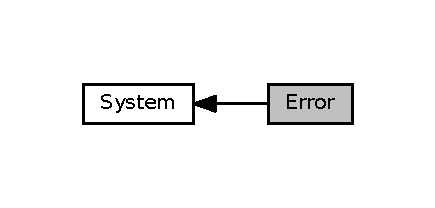
\includegraphics[width=209pt]{group__SYSTEM__ERROR}
\end{center}
\end{figure}
\subsection*{Macros}
\begin{DoxyCompactItemize}
\item 
\mbox{\Hypertarget{group__SYSTEM__ERROR_gae11b1d812e86d15ff7eef402ab14a522}\label{group__SYSTEM__ERROR_gae11b1d812e86d15ff7eef402ab14a522}} 
\#define {\bfseries S\+N\+\_\+\+S\+T\+A\+T\+U\+S\+\_\+\+B\+A\+SE}~0
\end{DoxyCompactItemize}
\subsection*{Typedefs}
\begin{DoxyCompactItemize}
\item 
typedef enum \hyperlink{group__SYSTEM__ERROR_ga8cb157fafd64d5b57cdc905615978e99}{sn\+\_\+status} \hyperlink{group__SYSTEM__ERROR_ga4540713b9a7a18ce44d78c3a10f7442f}{S\+N\+\_\+\+S\+T\+A\+T\+US}
\item 
\mbox{\Hypertarget{group__SYSTEM__ERROR_ga8052e9054a9f729dd6df474e52738add}\label{group__SYSTEM__ERROR_ga8052e9054a9f729dd6df474e52738add}} 
typedef int {\bfseries E\+R\+R\+O\+R\+\_\+T}
\end{DoxyCompactItemize}
\subsection*{Enumerations}
\begin{DoxyCompactItemize}
\item 
enum \hyperlink{group__SYSTEM__ERROR_ga8cb157fafd64d5b57cdc905615978e99}{sn\+\_\+status} \{ \newline
\hyperlink{group__SYSTEM__ERROR_gga8cb157fafd64d5b57cdc905615978e99a846b1bafe725017ec9e31883bd54a2b7}{S\+N\+\_\+\+S\+T\+A\+T\+U\+S\+\_\+\+OK} = (S\+N\+\_\+\+S\+T\+A\+T\+U\+S\+\_\+\+B\+A\+SE + 0), 
\hyperlink{group__SYSTEM__ERROR_gga8cb157fafd64d5b57cdc905615978e99a33a7a4a09ab240b76113b3b2df8f539c}{S\+N\+\_\+\+S\+T\+A\+T\+U\+S\+\_\+\+T\+I\+M\+E\+O\+UT}, 
\hyperlink{group__SYSTEM__ERROR_gga8cb157fafd64d5b57cdc905615978e99a86cc0e267ad9ae3a139250192918b190}{S\+N\+\_\+\+S\+T\+A\+T\+U\+S\+\_\+\+I\+N\+V\+A\+L\+I\+D\+\_\+\+P\+A\+R\+AM}, 
\hyperlink{group__SYSTEM__ERROR_gga8cb157fafd64d5b57cdc905615978e99ad828aa0b3ff9ee57cd21206608a057a7}{S\+N\+\_\+\+S\+T\+A\+T\+U\+S\+\_\+\+N\+O\+T\+\_\+\+S\+U\+P\+P\+O\+R\+T\+ED}, 
\newline
\hyperlink{group__SYSTEM__ERROR_gga8cb157fafd64d5b57cdc905615978e99ac7f7bdb5cc8a4aff8d350fe8914ddfac}{S\+N\+\_\+\+S\+T\+A\+T\+U\+S\+\_\+\+U\+N\+K\+N\+O\+W\+N\+\_\+\+M\+E\+S\+S\+A\+GE}, 
\hyperlink{group__SYSTEM__ERROR_gga8cb157fafd64d5b57cdc905615978e99a5b46a5ba5697471321165d636f445ef6}{S\+N\+\_\+\+S\+T\+A\+T\+U\+S\+\_\+\+O\+U\+T\+\_\+\+O\+F\+\_\+\+M\+EM}, 
\hyperlink{group__SYSTEM__ERROR_gga8cb157fafd64d5b57cdc905615978e99a12f634443b94c9897e3843a709e71e94}{S\+N\+\_\+\+S\+T\+A\+T\+U\+S\+\_\+\+N\+O\+T\+\_\+\+I\+N\+I\+T\+I\+A\+L\+I\+Z\+ED}, 
\hyperlink{group__SYSTEM__ERROR_gga8cb157fafd64d5b57cdc905615978e99a985eb387b42b31cf429a9b8084cb354c}{S\+N\+\_\+\+S\+T\+A\+T\+U\+S\+\_\+\+A\+L\+R\+E\+A\+D\+Y\+\_\+\+I\+N\+I\+T\+I\+A\+L\+I\+Z\+ED}, 
\newline
\hyperlink{group__SYSTEM__ERROR_gga8cb157fafd64d5b57cdc905615978e99a62a1abb5365baca1f3b9ae2713c97b92}{S\+N\+\_\+\+S\+T\+A\+T\+U\+S\+\_\+\+R\+E\+S\+O\+U\+R\+C\+E\+\_\+\+N\+O\+T\+\_\+\+A\+V\+A\+I\+L\+A\+B\+LE}, 
\hyperlink{group__SYSTEM__ERROR_gga8cb157fafd64d5b57cdc905615978e99a08cabf188f59fea3259d8e5822adc9be}{S\+N\+\_\+\+S\+T\+A\+T\+U\+S\+\_\+\+S\+D\+L\+\_\+\+E\+R\+R\+OR}, 
\hyperlink{group__SYSTEM__ERROR_gga8cb157fafd64d5b57cdc905615978e99a5fb3d22924030adb86d517fcb10859f8}{S\+N\+\_\+\+S\+T\+A\+T\+U\+S\+\_\+\+N\+O\+T\+\_\+\+OK}
 \}
\end{DoxyCompactItemize}
\subsection*{Error System}
\begin{DoxyCompactItemize}
\item 
void \hyperlink{group__SYSTEM__ERROR_ga0a87cb464a83646bf30c20c867754a02}{S\+N\+\_\+\+S\+Y\+S\+\_\+\+Error\+Check} (\hyperlink{group__SYSTEM__ERROR_ga4540713b9a7a18ce44d78c3a10f7442f}{S\+N\+\_\+\+S\+T\+A\+T\+US} error\+Status, const char $\ast$error\+Message, const char $\ast$\+\_\+file, const char $\ast$\+\_\+func, const int \+\_\+line)
\item 
void \hyperlink{group__SYSTEM__ERROR_gaacf422ec9176edcc5b0d803da0b567b7}{S\+N\+\_\+\+S\+Y\+S\+\_\+\+Log} (const char $\ast$log)
\item 
\#define \hyperlink{group__SYSTEM__ERROR_gaaa32db6b360e68cd1d2a84f7ac1992cd}{S\+N\+\_\+\+S\+Y\+S\+\_\+\+E\+R\+R\+O\+R\+\_\+\+C\+H\+E\+CK}(error,  msg)~\hyperlink{group__SYSTEM__ERROR_ga0a87cb464a83646bf30c20c867754a02}{S\+N\+\_\+\+S\+Y\+S\+\_\+\+Error\+Check}((error), (msg), \+\_\+\+\_\+\+F\+I\+L\+E\+\_\+\+\_\+, \+\_\+\+\_\+\+F\+U\+N\+C\+T\+I\+O\+N\+\_\+\+\_\+, \+\_\+\+\_\+\+L\+I\+N\+E\+\_\+\+\_\+)
\end{DoxyCompactItemize}


\subsection{Detailed Description}
System Error Functions. 



\subsection{Macro Definition Documentation}
\mbox{\Hypertarget{group__SYSTEM__ERROR_gaaa32db6b360e68cd1d2a84f7ac1992cd}\label{group__SYSTEM__ERROR_gaaa32db6b360e68cd1d2a84f7ac1992cd}} 
\index{Error@{Error}!S\+N\+\_\+\+S\+Y\+S\+\_\+\+E\+R\+R\+O\+R\+\_\+\+C\+H\+E\+CK@{S\+N\+\_\+\+S\+Y\+S\+\_\+\+E\+R\+R\+O\+R\+\_\+\+C\+H\+E\+CK}}
\index{S\+N\+\_\+\+S\+Y\+S\+\_\+\+E\+R\+R\+O\+R\+\_\+\+C\+H\+E\+CK@{S\+N\+\_\+\+S\+Y\+S\+\_\+\+E\+R\+R\+O\+R\+\_\+\+C\+H\+E\+CK}!Error@{Error}}
\subsubsection{\texorpdfstring{S\+N\+\_\+\+S\+Y\+S\+\_\+\+E\+R\+R\+O\+R\+\_\+\+C\+H\+E\+CK}{SN\_SYS\_ERROR\_CHECK}}
{\footnotesize\ttfamily \#define S\+N\+\_\+\+S\+Y\+S\+\_\+\+E\+R\+R\+O\+R\+\_\+\+C\+H\+E\+CK(\begin{DoxyParamCaption}\item[{}]{error,  }\item[{}]{msg }\end{DoxyParamCaption})~\hyperlink{group__SYSTEM__ERROR_ga0a87cb464a83646bf30c20c867754a02}{S\+N\+\_\+\+S\+Y\+S\+\_\+\+Error\+Check}((error), (msg), \+\_\+\+\_\+\+F\+I\+L\+E\+\_\+\+\_\+, \+\_\+\+\_\+\+F\+U\+N\+C\+T\+I\+O\+N\+\_\+\+\_\+, \+\_\+\+\_\+\+L\+I\+N\+E\+\_\+\+\_\+)}



{\ttfamily \#include $<$\hyperlink{SN__SYS__ERROR_8h}{S\+Y\+S\+T\+E\+M/\+I\+N\+C\+L\+U\+D\+E/\+S\+N\+\_\+\+S\+Y\+S\+\_\+\+E\+R\+R\+O\+R.\+h}$>$}


\begin{DoxyParams}{Parameters}
{\em error} & \\
\hline
{\em msg} & \\
\hline
\end{DoxyParams}
\begin{DoxyReturn}{Returns}
S\+N\+\_\+\+S\+T\+A\+T\+US 
\end{DoxyReturn}
\begin{DoxyNote}{Note}

\end{DoxyNote}


\subsection{Typedef Documentation}
\mbox{\Hypertarget{group__SYSTEM__ERROR_ga4540713b9a7a18ce44d78c3a10f7442f}\label{group__SYSTEM__ERROR_ga4540713b9a7a18ce44d78c3a10f7442f}} 
\index{Error@{Error}!S\+N\+\_\+\+S\+T\+A\+T\+US@{S\+N\+\_\+\+S\+T\+A\+T\+US}}
\index{S\+N\+\_\+\+S\+T\+A\+T\+US@{S\+N\+\_\+\+S\+T\+A\+T\+US}!Error@{Error}}
\subsubsection{\texorpdfstring{S\+N\+\_\+\+S\+T\+A\+T\+US}{SN\_STATUS}}
{\footnotesize\ttfamily typedef enum \hyperlink{group__SYSTEM__ERROR_ga8cb157fafd64d5b57cdc905615978e99}{sn\+\_\+status}  \hyperlink{group__SYSTEM__ERROR_ga4540713b9a7a18ce44d78c3a10f7442f}{S\+N\+\_\+\+S\+T\+A\+T\+US}}



{\ttfamily \#include $<$\hyperlink{SN__SYS__ERROR_8h}{S\+Y\+S\+T\+E\+M/\+I\+N\+C\+L\+U\+D\+E/\+S\+N\+\_\+\+S\+Y\+S\+\_\+\+E\+R\+R\+O\+R.\+h}$>$}

S\+N3D Error Code 

\subsection{Enumeration Type Documentation}
\mbox{\Hypertarget{group__SYSTEM__ERROR_ga8cb157fafd64d5b57cdc905615978e99}\label{group__SYSTEM__ERROR_ga8cb157fafd64d5b57cdc905615978e99}} 
\index{Error@{Error}!sn\+\_\+status@{sn\+\_\+status}}
\index{sn\+\_\+status@{sn\+\_\+status}!Error@{Error}}
\subsubsection{\texorpdfstring{sn\+\_\+status}{sn\_status}}
{\footnotesize\ttfamily enum \hyperlink{group__SYSTEM__ERROR_ga8cb157fafd64d5b57cdc905615978e99}{sn\+\_\+status}}



{\ttfamily \#include $<$\hyperlink{SN__SYS__ERROR_8h}{S\+Y\+S\+T\+E\+M/\+I\+N\+C\+L\+U\+D\+E/\+S\+N\+\_\+\+S\+Y\+S\+\_\+\+E\+R\+R\+O\+R.\+h}$>$}

\begin{DoxyEnumFields}{Enumerator}
\raisebox{\heightof{T}}[0pt][0pt]{\index{S\+N\+\_\+\+S\+T\+A\+T\+U\+S\+\_\+\+OK@{S\+N\+\_\+\+S\+T\+A\+T\+U\+S\+\_\+\+OK}!Error@{Error}}\index{Error@{Error}!S\+N\+\_\+\+S\+T\+A\+T\+U\+S\+\_\+\+OK@{S\+N\+\_\+\+S\+T\+A\+T\+U\+S\+\_\+\+OK}}}\mbox{\Hypertarget{group__SYSTEM__ERROR_gga8cb157fafd64d5b57cdc905615978e99a846b1bafe725017ec9e31883bd54a2b7}\label{group__SYSTEM__ERROR_gga8cb157fafd64d5b57cdc905615978e99a846b1bafe725017ec9e31883bd54a2b7}} 
S\+N\+\_\+\+S\+T\+A\+T\+U\+S\+\_\+\+OK&0 \\
\hline

\raisebox{\heightof{T}}[0pt][0pt]{\index{S\+N\+\_\+\+S\+T\+A\+T\+U\+S\+\_\+\+T\+I\+M\+E\+O\+UT@{S\+N\+\_\+\+S\+T\+A\+T\+U\+S\+\_\+\+T\+I\+M\+E\+O\+UT}!Error@{Error}}\index{Error@{Error}!S\+N\+\_\+\+S\+T\+A\+T\+U\+S\+\_\+\+T\+I\+M\+E\+O\+UT@{S\+N\+\_\+\+S\+T\+A\+T\+U\+S\+\_\+\+T\+I\+M\+E\+O\+UT}}}\mbox{\Hypertarget{group__SYSTEM__ERROR_gga8cb157fafd64d5b57cdc905615978e99a33a7a4a09ab240b76113b3b2df8f539c}\label{group__SYSTEM__ERROR_gga8cb157fafd64d5b57cdc905615978e99a33a7a4a09ab240b76113b3b2df8f539c}} 
S\+N\+\_\+\+S\+T\+A\+T\+U\+S\+\_\+\+T\+I\+M\+E\+O\+UT&1 \\
\hline

\raisebox{\heightof{T}}[0pt][0pt]{\index{S\+N\+\_\+\+S\+T\+A\+T\+U\+S\+\_\+\+I\+N\+V\+A\+L\+I\+D\+\_\+\+P\+A\+R\+AM@{S\+N\+\_\+\+S\+T\+A\+T\+U\+S\+\_\+\+I\+N\+V\+A\+L\+I\+D\+\_\+\+P\+A\+R\+AM}!Error@{Error}}\index{Error@{Error}!S\+N\+\_\+\+S\+T\+A\+T\+U\+S\+\_\+\+I\+N\+V\+A\+L\+I\+D\+\_\+\+P\+A\+R\+AM@{S\+N\+\_\+\+S\+T\+A\+T\+U\+S\+\_\+\+I\+N\+V\+A\+L\+I\+D\+\_\+\+P\+A\+R\+AM}}}\mbox{\Hypertarget{group__SYSTEM__ERROR_gga8cb157fafd64d5b57cdc905615978e99a86cc0e267ad9ae3a139250192918b190}\label{group__SYSTEM__ERROR_gga8cb157fafd64d5b57cdc905615978e99a86cc0e267ad9ae3a139250192918b190}} 
S\+N\+\_\+\+S\+T\+A\+T\+U\+S\+\_\+\+I\+N\+V\+A\+L\+I\+D\+\_\+\+P\+A\+R\+AM&2 \\
\hline

\raisebox{\heightof{T}}[0pt][0pt]{\index{S\+N\+\_\+\+S\+T\+A\+T\+U\+S\+\_\+\+N\+O\+T\+\_\+\+S\+U\+P\+P\+O\+R\+T\+ED@{S\+N\+\_\+\+S\+T\+A\+T\+U\+S\+\_\+\+N\+O\+T\+\_\+\+S\+U\+P\+P\+O\+R\+T\+ED}!Error@{Error}}\index{Error@{Error}!S\+N\+\_\+\+S\+T\+A\+T\+U\+S\+\_\+\+N\+O\+T\+\_\+\+S\+U\+P\+P\+O\+R\+T\+ED@{S\+N\+\_\+\+S\+T\+A\+T\+U\+S\+\_\+\+N\+O\+T\+\_\+\+S\+U\+P\+P\+O\+R\+T\+ED}}}\mbox{\Hypertarget{group__SYSTEM__ERROR_gga8cb157fafd64d5b57cdc905615978e99ad828aa0b3ff9ee57cd21206608a057a7}\label{group__SYSTEM__ERROR_gga8cb157fafd64d5b57cdc905615978e99ad828aa0b3ff9ee57cd21206608a057a7}} 
S\+N\+\_\+\+S\+T\+A\+T\+U\+S\+\_\+\+N\+O\+T\+\_\+\+S\+U\+P\+P\+O\+R\+T\+ED&3 \\
\hline

\raisebox{\heightof{T}}[0pt][0pt]{\index{S\+N\+\_\+\+S\+T\+A\+T\+U\+S\+\_\+\+U\+N\+K\+N\+O\+W\+N\+\_\+\+M\+E\+S\+S\+A\+GE@{S\+N\+\_\+\+S\+T\+A\+T\+U\+S\+\_\+\+U\+N\+K\+N\+O\+W\+N\+\_\+\+M\+E\+S\+S\+A\+GE}!Error@{Error}}\index{Error@{Error}!S\+N\+\_\+\+S\+T\+A\+T\+U\+S\+\_\+\+U\+N\+K\+N\+O\+W\+N\+\_\+\+M\+E\+S\+S\+A\+GE@{S\+N\+\_\+\+S\+T\+A\+T\+U\+S\+\_\+\+U\+N\+K\+N\+O\+W\+N\+\_\+\+M\+E\+S\+S\+A\+GE}}}\mbox{\Hypertarget{group__SYSTEM__ERROR_gga8cb157fafd64d5b57cdc905615978e99ac7f7bdb5cc8a4aff8d350fe8914ddfac}\label{group__SYSTEM__ERROR_gga8cb157fafd64d5b57cdc905615978e99ac7f7bdb5cc8a4aff8d350fe8914ddfac}} 
S\+N\+\_\+\+S\+T\+A\+T\+U\+S\+\_\+\+U\+N\+K\+N\+O\+W\+N\+\_\+\+M\+E\+S\+S\+A\+GE&4 \\
\hline

\raisebox{\heightof{T}}[0pt][0pt]{\index{S\+N\+\_\+\+S\+T\+A\+T\+U\+S\+\_\+\+O\+U\+T\+\_\+\+O\+F\+\_\+\+M\+EM@{S\+N\+\_\+\+S\+T\+A\+T\+U\+S\+\_\+\+O\+U\+T\+\_\+\+O\+F\+\_\+\+M\+EM}!Error@{Error}}\index{Error@{Error}!S\+N\+\_\+\+S\+T\+A\+T\+U\+S\+\_\+\+O\+U\+T\+\_\+\+O\+F\+\_\+\+M\+EM@{S\+N\+\_\+\+S\+T\+A\+T\+U\+S\+\_\+\+O\+U\+T\+\_\+\+O\+F\+\_\+\+M\+EM}}}\mbox{\Hypertarget{group__SYSTEM__ERROR_gga8cb157fafd64d5b57cdc905615978e99a5b46a5ba5697471321165d636f445ef6}\label{group__SYSTEM__ERROR_gga8cb157fafd64d5b57cdc905615978e99a5b46a5ba5697471321165d636f445ef6}} 
S\+N\+\_\+\+S\+T\+A\+T\+U\+S\+\_\+\+O\+U\+T\+\_\+\+O\+F\+\_\+\+M\+EM&5 \\
\hline

\raisebox{\heightof{T}}[0pt][0pt]{\index{S\+N\+\_\+\+S\+T\+A\+T\+U\+S\+\_\+\+N\+O\+T\+\_\+\+I\+N\+I\+T\+I\+A\+L\+I\+Z\+ED@{S\+N\+\_\+\+S\+T\+A\+T\+U\+S\+\_\+\+N\+O\+T\+\_\+\+I\+N\+I\+T\+I\+A\+L\+I\+Z\+ED}!Error@{Error}}\index{Error@{Error}!S\+N\+\_\+\+S\+T\+A\+T\+U\+S\+\_\+\+N\+O\+T\+\_\+\+I\+N\+I\+T\+I\+A\+L\+I\+Z\+ED@{S\+N\+\_\+\+S\+T\+A\+T\+U\+S\+\_\+\+N\+O\+T\+\_\+\+I\+N\+I\+T\+I\+A\+L\+I\+Z\+ED}}}\mbox{\Hypertarget{group__SYSTEM__ERROR_gga8cb157fafd64d5b57cdc905615978e99a12f634443b94c9897e3843a709e71e94}\label{group__SYSTEM__ERROR_gga8cb157fafd64d5b57cdc905615978e99a12f634443b94c9897e3843a709e71e94}} 
S\+N\+\_\+\+S\+T\+A\+T\+U\+S\+\_\+\+N\+O\+T\+\_\+\+I\+N\+I\+T\+I\+A\+L\+I\+Z\+ED&6 \\
\hline

\raisebox{\heightof{T}}[0pt][0pt]{\index{S\+N\+\_\+\+S\+T\+A\+T\+U\+S\+\_\+\+A\+L\+R\+E\+A\+D\+Y\+\_\+\+I\+N\+I\+T\+I\+A\+L\+I\+Z\+ED@{S\+N\+\_\+\+S\+T\+A\+T\+U\+S\+\_\+\+A\+L\+R\+E\+A\+D\+Y\+\_\+\+I\+N\+I\+T\+I\+A\+L\+I\+Z\+ED}!Error@{Error}}\index{Error@{Error}!S\+N\+\_\+\+S\+T\+A\+T\+U\+S\+\_\+\+A\+L\+R\+E\+A\+D\+Y\+\_\+\+I\+N\+I\+T\+I\+A\+L\+I\+Z\+ED@{S\+N\+\_\+\+S\+T\+A\+T\+U\+S\+\_\+\+A\+L\+R\+E\+A\+D\+Y\+\_\+\+I\+N\+I\+T\+I\+A\+L\+I\+Z\+ED}}}\mbox{\Hypertarget{group__SYSTEM__ERROR_gga8cb157fafd64d5b57cdc905615978e99a985eb387b42b31cf429a9b8084cb354c}\label{group__SYSTEM__ERROR_gga8cb157fafd64d5b57cdc905615978e99a985eb387b42b31cf429a9b8084cb354c}} 
S\+N\+\_\+\+S\+T\+A\+T\+U\+S\+\_\+\+A\+L\+R\+E\+A\+D\+Y\+\_\+\+I\+N\+I\+T\+I\+A\+L\+I\+Z\+ED&7 \\
\hline

\raisebox{\heightof{T}}[0pt][0pt]{\index{S\+N\+\_\+\+S\+T\+A\+T\+U\+S\+\_\+\+R\+E\+S\+O\+U\+R\+C\+E\+\_\+\+N\+O\+T\+\_\+\+A\+V\+A\+I\+L\+A\+B\+LE@{S\+N\+\_\+\+S\+T\+A\+T\+U\+S\+\_\+\+R\+E\+S\+O\+U\+R\+C\+E\+\_\+\+N\+O\+T\+\_\+\+A\+V\+A\+I\+L\+A\+B\+LE}!Error@{Error}}\index{Error@{Error}!S\+N\+\_\+\+S\+T\+A\+T\+U\+S\+\_\+\+R\+E\+S\+O\+U\+R\+C\+E\+\_\+\+N\+O\+T\+\_\+\+A\+V\+A\+I\+L\+A\+B\+LE@{S\+N\+\_\+\+S\+T\+A\+T\+U\+S\+\_\+\+R\+E\+S\+O\+U\+R\+C\+E\+\_\+\+N\+O\+T\+\_\+\+A\+V\+A\+I\+L\+A\+B\+LE}}}\mbox{\Hypertarget{group__SYSTEM__ERROR_gga8cb157fafd64d5b57cdc905615978e99a62a1abb5365baca1f3b9ae2713c97b92}\label{group__SYSTEM__ERROR_gga8cb157fafd64d5b57cdc905615978e99a62a1abb5365baca1f3b9ae2713c97b92}} 
S\+N\+\_\+\+S\+T\+A\+T\+U\+S\+\_\+\+R\+E\+S\+O\+U\+R\+C\+E\+\_\+\+N\+O\+T\+\_\+\+A\+V\+A\+I\+L\+A\+B\+LE&8 \\
\hline

\raisebox{\heightof{T}}[0pt][0pt]{\index{S\+N\+\_\+\+S\+T\+A\+T\+U\+S\+\_\+\+S\+D\+L\+\_\+\+E\+R\+R\+OR@{S\+N\+\_\+\+S\+T\+A\+T\+U\+S\+\_\+\+S\+D\+L\+\_\+\+E\+R\+R\+OR}!Error@{Error}}\index{Error@{Error}!S\+N\+\_\+\+S\+T\+A\+T\+U\+S\+\_\+\+S\+D\+L\+\_\+\+E\+R\+R\+OR@{S\+N\+\_\+\+S\+T\+A\+T\+U\+S\+\_\+\+S\+D\+L\+\_\+\+E\+R\+R\+OR}}}\mbox{\Hypertarget{group__SYSTEM__ERROR_gga8cb157fafd64d5b57cdc905615978e99a08cabf188f59fea3259d8e5822adc9be}\label{group__SYSTEM__ERROR_gga8cb157fafd64d5b57cdc905615978e99a08cabf188f59fea3259d8e5822adc9be}} 
S\+N\+\_\+\+S\+T\+A\+T\+U\+S\+\_\+\+S\+D\+L\+\_\+\+E\+R\+R\+OR&9 \\
\hline

\raisebox{\heightof{T}}[0pt][0pt]{\index{S\+N\+\_\+\+S\+T\+A\+T\+U\+S\+\_\+\+N\+O\+T\+\_\+\+OK@{S\+N\+\_\+\+S\+T\+A\+T\+U\+S\+\_\+\+N\+O\+T\+\_\+\+OK}!Error@{Error}}\index{Error@{Error}!S\+N\+\_\+\+S\+T\+A\+T\+U\+S\+\_\+\+N\+O\+T\+\_\+\+OK@{S\+N\+\_\+\+S\+T\+A\+T\+U\+S\+\_\+\+N\+O\+T\+\_\+\+OK}}}\mbox{\Hypertarget{group__SYSTEM__ERROR_gga8cb157fafd64d5b57cdc905615978e99a5fb3d22924030adb86d517fcb10859f8}\label{group__SYSTEM__ERROR_gga8cb157fafd64d5b57cdc905615978e99a5fb3d22924030adb86d517fcb10859f8}} 
S\+N\+\_\+\+S\+T\+A\+T\+U\+S\+\_\+\+N\+O\+T\+\_\+\+OK&10 \\
\hline

\end{DoxyEnumFields}


\subsection{Function Documentation}
\mbox{\Hypertarget{group__SYSTEM__ERROR_ga0a87cb464a83646bf30c20c867754a02}\label{group__SYSTEM__ERROR_ga0a87cb464a83646bf30c20c867754a02}} 
\index{Error@{Error}!S\+N\+\_\+\+S\+Y\+S\+\_\+\+Error\+Check@{S\+N\+\_\+\+S\+Y\+S\+\_\+\+Error\+Check}}
\index{S\+N\+\_\+\+S\+Y\+S\+\_\+\+Error\+Check@{S\+N\+\_\+\+S\+Y\+S\+\_\+\+Error\+Check}!Error@{Error}}
\subsubsection{\texorpdfstring{S\+N\+\_\+\+S\+Y\+S\+\_\+\+Error\+Check()}{SN\_SYS\_ErrorCheck()}}
{\footnotesize\ttfamily void S\+N\+\_\+\+S\+Y\+S\+\_\+\+Error\+Check (\begin{DoxyParamCaption}\item[{\hyperlink{group__SYSTEM__ERROR_ga4540713b9a7a18ce44d78c3a10f7442f}{S\+N\+\_\+\+S\+T\+A\+T\+US}}]{error\+Status,  }\item[{const char $\ast$}]{error\+Message,  }\item[{const char $\ast$}]{\+\_\+file,  }\item[{const char $\ast$}]{\+\_\+func,  }\item[{const int}]{\+\_\+line }\end{DoxyParamCaption})}



{\ttfamily \#include $<$\hyperlink{SN__SYS__ERROR_8h}{S\+Y\+S\+T\+E\+M/\+I\+N\+C\+L\+U\+D\+E/\+S\+N\+\_\+\+S\+Y\+S\+\_\+\+E\+R\+R\+O\+R.\+h}$>$}


\begin{DoxyParams}{Parameters}
{\em error\+Status} & \\
\hline
{\em error\+Meesage} & \\
\hline
{\em \+\_\+file} & \\
\hline
{\em \+\_\+func} & \\
\hline
{\em \+\_\+line} & \\
\hline
\end{DoxyParams}
\begin{DoxyReturn}{Returns}
S\+N\+\_\+\+S\+T\+A\+T\+US 
\end{DoxyReturn}
\begin{DoxyNote}{Note}

\end{DoxyNote}
\mbox{\Hypertarget{group__SYSTEM__ERROR_gaacf422ec9176edcc5b0d803da0b567b7}\label{group__SYSTEM__ERROR_gaacf422ec9176edcc5b0d803da0b567b7}} 
\index{Error@{Error}!S\+N\+\_\+\+S\+Y\+S\+\_\+\+Log@{S\+N\+\_\+\+S\+Y\+S\+\_\+\+Log}}
\index{S\+N\+\_\+\+S\+Y\+S\+\_\+\+Log@{S\+N\+\_\+\+S\+Y\+S\+\_\+\+Log}!Error@{Error}}
\subsubsection{\texorpdfstring{S\+N\+\_\+\+S\+Y\+S\+\_\+\+Log()}{SN\_SYS\_Log()}}
{\footnotesize\ttfamily void S\+N\+\_\+\+S\+Y\+S\+\_\+\+Log (\begin{DoxyParamCaption}\item[{const char $\ast$}]{log }\end{DoxyParamCaption})}



{\ttfamily \#include $<$\hyperlink{SN__SYS__ERROR_8h}{S\+Y\+S\+T\+E\+M/\+I\+N\+C\+L\+U\+D\+E/\+S\+N\+\_\+\+S\+Y\+S\+\_\+\+E\+R\+R\+O\+R.\+h}$>$}


\begin{DoxyParams}{Parameters}
{\em log} & \\
\hline
\end{DoxyParams}
\begin{DoxyReturn}{Returns}
S\+N\+\_\+\+S\+T\+A\+T\+US 
\end{DoxyReturn}
\begin{DoxyNote}{Note}

\end{DoxyNote}


���}	� �
����DEV��INO��SYN��SV~�#`�
#`�
�#`�
k���=I]�[r�

���}	� �
����DEV��INO��SYN��SV~�#`_�#`_�#`_�k��"�I]�[w;
\hypertarget{group__SYSTEM__TIMER}{}\section{Timer}
\label{group__SYSTEM__TIMER}\index{Timer@{Timer}}


System Timer Functions.  


Collaboration diagram for Timer\+:\nopagebreak
\begin{figure}[H]
\begin{center}
\leavevmode
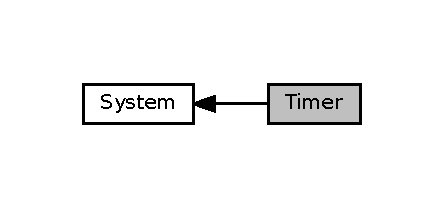
\includegraphics[width=213pt]{group__SYSTEM__TIMER}
\end{center}
\end{figure}
\subsection*{Classes}
\begin{DoxyCompactItemize}
\item 
struct \hyperlink{structsys__timer__id}{sys\+\_\+timer\+\_\+id}
\end{DoxyCompactItemize}
\subsection*{Macros}
\begin{DoxyCompactItemize}
\item 
\#define \hyperlink{group__SYSTEM__TIMER_gad99ad563a1a632fde508ad8be6422e57}{M\+A\+X\+\_\+\+N\+U\+M\+\_\+\+O\+F\+\_\+\+T\+SR}~32
\item 
\mbox{\Hypertarget{group__SYSTEM__TIMER_ga3ab2d3270619515d0cfdc5caf09d6366}\label{group__SYSTEM__TIMER_ga3ab2d3270619515d0cfdc5caf09d6366}} 
\#define {\bfseries U\+N\+A\+L\+L\+O\+C\+A\+T\+E\+D\+\_\+\+T\+S\+R\+\_\+\+ID}~(0x\+F\+F\+F\+F\+F\+F\+F\+F)
\end{DoxyCompactItemize}
\subsection*{Typedefs}
\begin{DoxyCompactItemize}
\item 
\mbox{\Hypertarget{group__SYSTEM__TIMER_ga0964d5651c1e8775bdedb28ad089d8b9}\label{group__SYSTEM__TIMER_ga0964d5651c1e8775bdedb28ad089d8b9}} 
typedef struct \hyperlink{structsys__timer__id}{sys\+\_\+timer\+\_\+id} {\bfseries sys\+Timer\+Q\+\_\+t}
\item 
\mbox{\Hypertarget{group__SYSTEM__TIMER_ga45dfe75dba9f4d77371435e6ea122117}\label{group__SYSTEM__TIMER_ga45dfe75dba9f4d77371435e6ea122117}} 
typedef uint32\+\_\+t {\bfseries sys\+Timer\+Id\+\_\+t}
\end{DoxyCompactItemize}
\subsection*{Functions}
\begin{DoxyCompactItemize}
\item 
\mbox{\Hypertarget{group__SYSTEM__TIMER_gabe15a62b1e228b796d3a2297c085c9ef}\label{group__SYSTEM__TIMER_gabe15a62b1e228b796d3a2297c085c9ef}} 
\hyperlink{group__SYSTEM__ERROR_ga4540713b9a7a18ce44d78c3a10f7442f}{S\+N\+\_\+\+S\+T\+A\+T\+US} {\bfseries S\+N\+\_\+\+S\+Y\+S\+\_\+\+Timer\+Init} (void)
\item 
\mbox{\Hypertarget{group__SYSTEM__TIMER_ga1d85ad6b65ffc1c7a3fd35361b33aa08}\label{group__SYSTEM__TIMER_ga1d85ad6b65ffc1c7a3fd35361b33aa08}} 
\hyperlink{group__SYSTEM__ERROR_ga4540713b9a7a18ce44d78c3a10f7442f}{S\+N\+\_\+\+S\+T\+A\+T\+US} {\bfseries S\+N\+\_\+\+S\+Y\+S\+\_\+\+Timer\+Create} (sys\+Timer\+Id\+\_\+t $\ast$p\+Id\+T\+SR, unsigned int ms\+Duration, void $\ast$pf\+T\+SR)
\item 
\mbox{\Hypertarget{group__SYSTEM__TIMER_gaa004347fdd0940a882a77729feaf60c4}\label{group__SYSTEM__TIMER_gaa004347fdd0940a882a77729feaf60c4}} 
\hyperlink{group__SYSTEM__ERROR_ga4540713b9a7a18ce44d78c3a10f7442f}{S\+N\+\_\+\+S\+T\+A\+T\+US} {\bfseries S\+N\+\_\+\+S\+Y\+S\+\_\+\+Timer\+Cancle} (sys\+Timer\+Id\+\_\+t $\ast$p\+Id\+T\+SR)
\item 
\mbox{\Hypertarget{group__SYSTEM__TIMER_ga4cf64b0280d940416955ba171ed339aa}\label{group__SYSTEM__TIMER_ga4cf64b0280d940416955ba171ed339aa}} 
\hyperlink{group__SYSTEM__ERROR_ga4540713b9a7a18ce44d78c3a10f7442f}{S\+N\+\_\+\+S\+T\+A\+T\+US} {\bfseries S\+N\+\_\+\+S\+Y\+S\+\_\+\+Delay} (uint32\+\_\+t msec)
\end{DoxyCompactItemize}


\subsection{Detailed Description}
System Timer Functions. 



\subsection{Macro Definition Documentation}
\mbox{\Hypertarget{group__SYSTEM__TIMER_gad99ad563a1a632fde508ad8be6422e57}\label{group__SYSTEM__TIMER_gad99ad563a1a632fde508ad8be6422e57}} 
\index{Timer@{Timer}!M\+A\+X\+\_\+\+N\+U\+M\+\_\+\+O\+F\+\_\+\+T\+SR@{M\+A\+X\+\_\+\+N\+U\+M\+\_\+\+O\+F\+\_\+\+T\+SR}}
\index{M\+A\+X\+\_\+\+N\+U\+M\+\_\+\+O\+F\+\_\+\+T\+SR@{M\+A\+X\+\_\+\+N\+U\+M\+\_\+\+O\+F\+\_\+\+T\+SR}!Timer@{Timer}}
\subsubsection{\texorpdfstring{M\+A\+X\+\_\+\+N\+U\+M\+\_\+\+O\+F\+\_\+\+T\+SR}{MAX\_NUM\_OF\_TSR}}
{\footnotesize\ttfamily \#define M\+A\+X\+\_\+\+N\+U\+M\+\_\+\+O\+F\+\_\+\+T\+SR~32}



{\ttfamily \#include $<$\hyperlink{SN__SYS__TIMER_8h}{S\+Y\+S\+T\+E\+M/\+I\+N\+C\+L\+U\+D\+E/\+S\+N\+\_\+\+S\+Y\+S\+\_\+\+T\+I\+M\+E\+R.\+h}$>$}

Static Define 
\hypertarget{group__SYSTEM__USB__DRIVER}{}\section{U\+SB Driver}
\label{group__SYSTEM__USB__DRIVER}\index{U\+S\+B Driver@{U\+S\+B Driver}}


System U\+SB Driver Functions.  


Collaboration diagram for U\+SB Driver\+:\nopagebreak
\begin{figure}[H]
\begin{center}
\leavevmode
\includegraphics[width=238pt]{group__SYSTEM__USB__DRIVER}
\end{center}
\end{figure}
\subsection*{Classes}
\begin{DoxyCompactItemize}
\item 
struct \hyperlink{structusb__dev__handle}{usb\+\_\+dev\+\_\+handle}
\end{DoxyCompactItemize}
\subsection*{U\+SB Event Macro}
\begin{DoxyCompactItemize}
\item 
\mbox{\Hypertarget{group__SYSTEM__USB__DRIVER_ga9b9388bbbf745b6cff8609792c63490d}\label{group__SYSTEM__USB__DRIVER_ga9b9388bbbf745b6cff8609792c63490d}} 
enum {\bfseries usb\+\_\+driver\+\_\+event} \{ {\bfseries M\+S\+G\+\_\+\+U\+S\+B\+\_\+\+E\+V\+T\+\_\+\+M\+O\+U\+NT} = 0x01, 
{\bfseries M\+S\+G\+\_\+\+U\+S\+B\+\_\+\+E\+V\+T\+\_\+\+U\+N\+M\+O\+U\+NT} = 0x02, 
{\bfseries M\+S\+G\+\_\+\+U\+S\+B\+\_\+\+E\+V\+T\+\_\+\+W\+A\+I\+T\+I\+NG} = 0x03, 
{\bfseries M\+S\+G\+\_\+\+S\+B\+\_\+\+E\+V\+T\+\_\+\+N\+O\+NE} = 0x04
 \}
\item 
\mbox{\Hypertarget{group__SYSTEM__USB__DRIVER_ga1bee7d22386716ee60aef5b482b5fa7e}\label{group__SYSTEM__USB__DRIVER_ga1bee7d22386716ee60aef5b482b5fa7e}} 
enum usb\+\_\+driver\+\_\+event {\bfseries usb\+Evt\+\_\+t}
\end{DoxyCompactItemize}
\subsection*{U\+SB Driver System}
\label{_amgrp520fea60abf54d62f341eebb2a0145c6}%
Description of Serial System Init and Uninit funtions. \begin{DoxyCompactItemize}
\item 
\hyperlink{group__SYSTEM__ERROR_ga4540713b9a7a18ce44d78c3a10f7442f}{S\+N\+\_\+\+S\+T\+A\+T\+US} \hyperlink{group__SYSTEM__USB__DRIVER_gaf7719b8e9f6d6f05b702ac7d4e9c5a61}{S\+N\+\_\+\+S\+Y\+S\+\_\+\+U\+S\+B\+Driver\+Init} (void $\ast$(pf\+Call\+Back)(int evt))
\item 
\hyperlink{group__SYSTEM__ERROR_ga4540713b9a7a18ce44d78c3a10f7442f}{S\+N\+\_\+\+S\+T\+A\+T\+US} \hyperlink{group__SYSTEM__USB__DRIVER_ga60bc7a83a5370d89dffe6e3d4ad88538}{S\+N\+\_\+\+S\+Y\+S\+\_\+\+U\+S\+B\+Driver\+Terminate} (void)
\end{DoxyCompactItemize}
\subsection*{U\+SB Driver System \+:\+: Util}
\label{_amgrp0bffd34c90f12d85c8fa16d1d16b13fd}%
Description of Serial System Init and Uninit funtions. \begin{DoxyCompactItemize}
\item 
bool \hyperlink{group__SYSTEM__USB__DRIVER_gaccafd3f2c96104a41f768f05a083226f}{S\+N\+\_\+\+S\+Y\+S\+\_\+\+U\+S\+B\+Driver\+Is\+Mount} (void)
\end{DoxyCompactItemize}


\subsection{Detailed Description}
System U\+SB Driver Functions. 



\subsection{Function Documentation}
\mbox{\Hypertarget{group__SYSTEM__USB__DRIVER_gaf7719b8e9f6d6f05b702ac7d4e9c5a61}\label{group__SYSTEM__USB__DRIVER_gaf7719b8e9f6d6f05b702ac7d4e9c5a61}} 
\index{U\+S\+B Driver@{U\+S\+B Driver}!S\+N\+\_\+\+S\+Y\+S\+\_\+\+U\+S\+B\+Driver\+Init@{S\+N\+\_\+\+S\+Y\+S\+\_\+\+U\+S\+B\+Driver\+Init}}
\index{S\+N\+\_\+\+S\+Y\+S\+\_\+\+U\+S\+B\+Driver\+Init@{S\+N\+\_\+\+S\+Y\+S\+\_\+\+U\+S\+B\+Driver\+Init}!U\+S\+B Driver@{U\+S\+B Driver}}
\subsubsection{\texorpdfstring{S\+N\+\_\+\+S\+Y\+S\+\_\+\+U\+S\+B\+Driver\+Init()}{SN\_SYS\_USBDriverInit()}}
{\footnotesize\ttfamily \hyperlink{group__SYSTEM__ERROR_ga4540713b9a7a18ce44d78c3a10f7442f}{S\+N\+\_\+\+S\+T\+A\+T\+US} S\+N\+\_\+\+S\+Y\+S\+\_\+\+U\+S\+B\+Driver\+Init (\begin{DoxyParamCaption}\item[{void $\ast$}]{pf\+Call\+Back)(int evt }\end{DoxyParamCaption})}



{\ttfamily \#include $<$\hyperlink{SN__SYS__USB__DRIVER_8h}{S\+Y\+S\+T\+E\+M/\+I\+N\+C\+L\+U\+D\+E/\+S\+N\+\_\+\+S\+Y\+S\+\_\+\+U\+S\+B\+\_\+\+D\+R\+I\+V\+E\+R.\+h}$>$}


\begin{DoxyParams}{Parameters}
{\em pf\+Call\+Back} & \\
\hline
\end{DoxyParams}
\begin{DoxyReturn}{Returns}
S\+N\+\_\+\+S\+T\+A\+T\+US 
\end{DoxyReturn}
\begin{DoxyNote}{Note}

\end{DoxyNote}
\mbox{\Hypertarget{group__SYSTEM__USB__DRIVER_gaccafd3f2c96104a41f768f05a083226f}\label{group__SYSTEM__USB__DRIVER_gaccafd3f2c96104a41f768f05a083226f}} 
\index{U\+S\+B Driver@{U\+S\+B Driver}!S\+N\+\_\+\+S\+Y\+S\+\_\+\+U\+S\+B\+Driver\+Is\+Mount@{S\+N\+\_\+\+S\+Y\+S\+\_\+\+U\+S\+B\+Driver\+Is\+Mount}}
\index{S\+N\+\_\+\+S\+Y\+S\+\_\+\+U\+S\+B\+Driver\+Is\+Mount@{S\+N\+\_\+\+S\+Y\+S\+\_\+\+U\+S\+B\+Driver\+Is\+Mount}!U\+S\+B Driver@{U\+S\+B Driver}}
\subsubsection{\texorpdfstring{S\+N\+\_\+\+S\+Y\+S\+\_\+\+U\+S\+B\+Driver\+Is\+Mount()}{SN\_SYS\_USBDriverIsMount()}}
{\footnotesize\ttfamily bool S\+N\+\_\+\+S\+Y\+S\+\_\+\+U\+S\+B\+Driver\+Is\+Mount (\begin{DoxyParamCaption}\item[{void}]{ }\end{DoxyParamCaption})}



{\ttfamily \#include $<$\hyperlink{SN__SYS__USB__DRIVER_8h}{S\+Y\+S\+T\+E\+M/\+I\+N\+C\+L\+U\+D\+E/\+S\+N\+\_\+\+S\+Y\+S\+\_\+\+U\+S\+B\+\_\+\+D\+R\+I\+V\+E\+R.\+h}$>$}

\begin{DoxyReturn}{Returns}
is\+Mount 
\end{DoxyReturn}
\begin{DoxyNote}{Note}

\end{DoxyNote}
\mbox{\Hypertarget{group__SYSTEM__USB__DRIVER_ga60bc7a83a5370d89dffe6e3d4ad88538}\label{group__SYSTEM__USB__DRIVER_ga60bc7a83a5370d89dffe6e3d4ad88538}} 
\index{U\+S\+B Driver@{U\+S\+B Driver}!S\+N\+\_\+\+S\+Y\+S\+\_\+\+U\+S\+B\+Driver\+Terminate@{S\+N\+\_\+\+S\+Y\+S\+\_\+\+U\+S\+B\+Driver\+Terminate}}
\index{S\+N\+\_\+\+S\+Y\+S\+\_\+\+U\+S\+B\+Driver\+Terminate@{S\+N\+\_\+\+S\+Y\+S\+\_\+\+U\+S\+B\+Driver\+Terminate}!U\+S\+B Driver@{U\+S\+B Driver}}
\subsubsection{\texorpdfstring{S\+N\+\_\+\+S\+Y\+S\+\_\+\+U\+S\+B\+Driver\+Terminate()}{SN\_SYS\_USBDriverTerminate()}}
{\footnotesize\ttfamily \hyperlink{group__SYSTEM__ERROR_ga4540713b9a7a18ce44d78c3a10f7442f}{S\+N\+\_\+\+S\+T\+A\+T\+US} S\+N\+\_\+\+S\+Y\+S\+\_\+\+U\+S\+B\+Driver\+Terminate (\begin{DoxyParamCaption}\item[{void}]{ }\end{DoxyParamCaption})}



{\ttfamily \#include $<$\hyperlink{SN__SYS__USB__DRIVER_8h}{S\+Y\+S\+T\+E\+M/\+I\+N\+C\+L\+U\+D\+E/\+S\+N\+\_\+\+S\+Y\+S\+\_\+\+U\+S\+B\+\_\+\+D\+R\+I\+V\+E\+R.\+h}$>$}

\begin{DoxyReturn}{Returns}
S\+N\+\_\+\+S\+T\+A\+T\+US 
\end{DoxyReturn}
\begin{DoxyNote}{Note}

\end{DoxyNote}

\hypertarget{group__APP}{}\section{Application}
\label{group__APP}\index{Application@{Application}}
Collaboration diagram for Application\+:
\nopagebreak
\begin{figure}[H]
\begin{center}
\leavevmode
\includegraphics[width=300pt]{group__APP}
\end{center}
\end{figure}
\subsection*{Modules}
\begin{DoxyCompactItemize}
\item 
\hyperlink{group__APP__MSG}{Application Message}
\begin{DoxyCompactList}\small\item\em Application Message Type and messages. \end{DoxyCompactList}\end{DoxyCompactItemize}


\subsection{Detailed Description}

\hypertarget{group__MODULE__3D__PRINTER}{}\section{3D Printer}
\label{group__MODULE__3D__PRINTER}\index{3\+D Printer@{3\+D Printer}}


3D Printer Module Functions.  


Collaboration diagram for 3D Printer\+:\nopagebreak
\begin{figure}[H]
\begin{center}
\leavevmode
\includegraphics[width=232pt]{group__MODULE__3D__PRINTER}
\end{center}
\end{figure}
\subsection*{Functions}
\begin{DoxyCompactItemize}
\item 
\mbox{\Hypertarget{group__MODULE__3D__PRINTER_ga31f1d937f766fc6699b39b625a10aaa5}\label{group__MODULE__3D__PRINTER_ga31f1d937f766fc6699b39b625a10aaa5}} 
\hyperlink{group__SYSTEM__ERROR_ga4540713b9a7a18ce44d78c3a10f7442f}{S\+N\+\_\+\+S\+T\+A\+T\+US} {\bfseries S\+N\+\_\+\+M\+O\+D\+U\+L\+E\+\_\+3\+D\+\_\+\+P\+R\+I\+N\+T\+E\+R\+\_\+\+Test} (void)
\end{DoxyCompactItemize}
\subsection*{3D Printr Module}
\label{_amgrp31919ac2a63e9801f2c4fb221e60d48f}%
Description of 3D Printr Module Init and Uninit funtions. \begin{DoxyCompactItemize}
\item 
\hyperlink{group__SYSTEM__ERROR_ga4540713b9a7a18ce44d78c3a10f7442f}{S\+N\+\_\+\+S\+T\+A\+T\+US} \hyperlink{group__MODULE__3D__PRINTER_ga801e265ffe6f8c56081112f4fdd35f39}{S\+N\+\_\+\+M\+O\+D\+U\+L\+E\+\_\+3\+D\+\_\+\+P\+R\+I\+N\+T\+E\+R\+\_\+\+Init} (void)
\item 
\hyperlink{group__SYSTEM__ERROR_ga4540713b9a7a18ce44d78c3a10f7442f}{S\+N\+\_\+\+S\+T\+A\+T\+US} \hyperlink{group__MODULE__3D__PRINTER_ga776f5e31b0c0e176e35669f9432baec0}{S\+N\+\_\+\+M\+O\+D\+U\+L\+E\+\_\+3\+D\+\_\+\+P\+R\+I\+N\+T\+E\+R\+\_\+\+Uninit} (void)
\end{DoxyCompactItemize}
\subsection*{3D Printer Module \+:\+: Printing.}
\label{_amgrpc4945650ed87e7ed89ffb690e375bfb1}%
Description of 3D Printr Module funtions. \begin{DoxyCompactItemize}
\item 
\hyperlink{group__SYSTEM__ERROR_ga4540713b9a7a18ce44d78c3a10f7442f}{S\+N\+\_\+\+S\+T\+A\+T\+US} \hyperlink{group__MODULE__3D__PRINTER_ga439ebb10f8ee839218655c5177e9110b}{S\+N\+\_\+\+M\+O\+D\+U\+L\+E\+\_\+3\+D\+\_\+\+P\+R\+I\+N\+T\+E\+R\+\_\+\+Start} (uint32\+\_\+t page\+Index, uint32\+\_\+t item\+Index)
\item 
\hyperlink{group__SYSTEM__ERROR_ga4540713b9a7a18ce44d78c3a10f7442f}{S\+N\+\_\+\+S\+T\+A\+T\+US} \hyperlink{group__MODULE__3D__PRINTER_ga21ca69a451fafe2c9218c9a1737e1f15}{S\+N\+\_\+\+M\+O\+D\+U\+L\+E\+\_\+3\+D\+\_\+\+P\+R\+I\+N\+T\+E\+R\+\_\+\+Stop} (void)
\item 
\hyperlink{group__SYSTEM__ERROR_ga4540713b9a7a18ce44d78c3a10f7442f}{S\+N\+\_\+\+S\+T\+A\+T\+US} \hyperlink{group__MODULE__3D__PRINTER_ga84a03238ddc0021011c12839757bf8c2}{S\+N\+\_\+\+M\+O\+D\+U\+L\+E\+\_\+3\+D\+\_\+\+P\+R\+I\+N\+T\+E\+R\+\_\+\+Pause} (void)
\item 
\hyperlink{group__SYSTEM__ERROR_ga4540713b9a7a18ce44d78c3a10f7442f}{S\+N\+\_\+\+S\+T\+A\+T\+US} \hyperlink{group__MODULE__3D__PRINTER_gaabec8b5f01119d989d725eff26053ca5}{S\+N\+\_\+\+M\+O\+D\+U\+L\+E\+\_\+3\+D\+\_\+\+P\+R\+I\+N\+T\+E\+R\+\_\+\+Resume} (void)
\end{DoxyCompactItemize}
\subsection*{3D Printer Module \+:\+: Z Control.}
\label{_amgrp0b5aafc53c5099dcb4016e710d2ae272}%
Description of 3D Printr Module funtions. \begin{DoxyCompactItemize}
\item 
\hyperlink{group__SYSTEM__ERROR_ga4540713b9a7a18ce44d78c3a10f7442f}{S\+N\+\_\+\+S\+T\+A\+T\+US} \hyperlink{group__MODULE__3D__PRINTER_ga83ec7a117b45a5760e1aecde26f69dea}{S\+N\+\_\+\+M\+O\+D\+U\+L\+E\+\_\+3\+D\+\_\+\+P\+R\+I\+N\+T\+E\+R\+\_\+\+Motor\+Init} (void)
\item 
\hyperlink{group__SYSTEM__ERROR_ga4540713b9a7a18ce44d78c3a10f7442f}{S\+N\+\_\+\+S\+T\+A\+T\+US} \hyperlink{group__MODULE__3D__PRINTER_ga2f644e451b310348d50fef6c762bbbcc}{S\+N\+\_\+\+M\+O\+D\+U\+L\+E\+\_\+3\+D\+\_\+\+P\+R\+I\+N\+T\+E\+R\+\_\+\+Motor\+Uninit} (void)
\item 
\hyperlink{group__SYSTEM__ERROR_ga4540713b9a7a18ce44d78c3a10f7442f}{S\+N\+\_\+\+S\+T\+A\+T\+US} \hyperlink{group__MODULE__3D__PRINTER_ga7bba4aa3966da87ac001b67b301310c1}{S\+N\+\_\+\+M\+O\+D\+U\+L\+E\+\_\+3\+D\+\_\+\+P\+R\+I\+N\+T\+E\+R\+\_\+\+Z\+\_\+\+Homing} (void)
\item 
\hyperlink{group__SYSTEM__ERROR_ga4540713b9a7a18ce44d78c3a10f7442f}{S\+N\+\_\+\+S\+T\+A\+T\+US} \hyperlink{group__MODULE__3D__PRINTER_ga47326e9f9d52dae584ee7c12011efc64}{S\+N\+\_\+\+M\+O\+D\+U\+L\+E\+\_\+3\+D\+\_\+\+P\+R\+I\+N\+T\+E\+R\+\_\+\+Z\+\_\+\+Up} (float mm)
\item 
\hyperlink{group__SYSTEM__ERROR_ga4540713b9a7a18ce44d78c3a10f7442f}{S\+N\+\_\+\+S\+T\+A\+T\+US} \hyperlink{group__MODULE__3D__PRINTER_ga65e82d5d94b534427c5d036080e77cf0}{S\+N\+\_\+\+M\+O\+D\+U\+L\+E\+\_\+3\+D\+\_\+\+P\+R\+I\+N\+T\+E\+R\+\_\+\+Z\+\_\+\+Down} (float mm)
\end{DoxyCompactItemize}


\subsection{Detailed Description}
3D Printer Module Functions. 



\subsection{Function Documentation}
\mbox{\Hypertarget{group__MODULE__3D__PRINTER_ga801e265ffe6f8c56081112f4fdd35f39}\label{group__MODULE__3D__PRINTER_ga801e265ffe6f8c56081112f4fdd35f39}} 
\index{3\+D Printer@{3\+D Printer}!S\+N\+\_\+\+M\+O\+D\+U\+L\+E\+\_\+3\+D\+\_\+\+P\+R\+I\+N\+T\+E\+R\+\_\+\+Init@{S\+N\+\_\+\+M\+O\+D\+U\+L\+E\+\_\+3\+D\+\_\+\+P\+R\+I\+N\+T\+E\+R\+\_\+\+Init}}
\index{S\+N\+\_\+\+M\+O\+D\+U\+L\+E\+\_\+3\+D\+\_\+\+P\+R\+I\+N\+T\+E\+R\+\_\+\+Init@{S\+N\+\_\+\+M\+O\+D\+U\+L\+E\+\_\+3\+D\+\_\+\+P\+R\+I\+N\+T\+E\+R\+\_\+\+Init}!3\+D Printer@{3\+D Printer}}
\subsubsection{\texorpdfstring{S\+N\+\_\+\+M\+O\+D\+U\+L\+E\+\_\+3\+D\+\_\+\+P\+R\+I\+N\+T\+E\+R\+\_\+\+Init()}{SN\_MODULE\_3D\_PRINTER\_Init()}}
{\footnotesize\ttfamily \hyperlink{group__SYSTEM__ERROR_ga4540713b9a7a18ce44d78c3a10f7442f}{S\+N\+\_\+\+S\+T\+A\+T\+US} S\+N\+\_\+\+M\+O\+D\+U\+L\+E\+\_\+3\+D\+\_\+\+P\+R\+I\+N\+T\+E\+R\+\_\+\+Init (\begin{DoxyParamCaption}\item[{void}]{ }\end{DoxyParamCaption})}



{\ttfamily \#include $<$\hyperlink{SN__MODULE__3D__PRINTER_8h}{M\+O\+D\+U\+L\+E/\+I\+N\+C\+L\+U\+D\+E/\+S\+N\+\_\+\+M\+O\+D\+U\+L\+E\+\_\+3\+D\+\_\+\+P\+R\+I\+N\+T\+E\+R.\+h}$>$}

\begin{DoxyReturn}{Returns}
S\+N\+\_\+\+S\+T\+A\+T\+US
\end{DoxyReturn}
\begin{DoxyNote}{Note}

\end{DoxyNote}
\mbox{\Hypertarget{group__MODULE__3D__PRINTER_ga83ec7a117b45a5760e1aecde26f69dea}\label{group__MODULE__3D__PRINTER_ga83ec7a117b45a5760e1aecde26f69dea}} 
\index{3\+D Printer@{3\+D Printer}!S\+N\+\_\+\+M\+O\+D\+U\+L\+E\+\_\+3\+D\+\_\+\+P\+R\+I\+N\+T\+E\+R\+\_\+\+Motor\+Init@{S\+N\+\_\+\+M\+O\+D\+U\+L\+E\+\_\+3\+D\+\_\+\+P\+R\+I\+N\+T\+E\+R\+\_\+\+Motor\+Init}}
\index{S\+N\+\_\+\+M\+O\+D\+U\+L\+E\+\_\+3\+D\+\_\+\+P\+R\+I\+N\+T\+E\+R\+\_\+\+Motor\+Init@{S\+N\+\_\+\+M\+O\+D\+U\+L\+E\+\_\+3\+D\+\_\+\+P\+R\+I\+N\+T\+E\+R\+\_\+\+Motor\+Init}!3\+D Printer@{3\+D Printer}}
\subsubsection{\texorpdfstring{S\+N\+\_\+\+M\+O\+D\+U\+L\+E\+\_\+3\+D\+\_\+\+P\+R\+I\+N\+T\+E\+R\+\_\+\+Motor\+Init()}{SN\_MODULE\_3D\_PRINTER\_MotorInit()}}
{\footnotesize\ttfamily \hyperlink{group__SYSTEM__ERROR_ga4540713b9a7a18ce44d78c3a10f7442f}{S\+N\+\_\+\+S\+T\+A\+T\+US} S\+N\+\_\+\+M\+O\+D\+U\+L\+E\+\_\+3\+D\+\_\+\+P\+R\+I\+N\+T\+E\+R\+\_\+\+Motor\+Init (\begin{DoxyParamCaption}\item[{void}]{ }\end{DoxyParamCaption})}



{\ttfamily \#include $<$\hyperlink{SN__MODULE__3D__PRINTER_8h}{M\+O\+D\+U\+L\+E/\+I\+N\+C\+L\+U\+D\+E/\+S\+N\+\_\+\+M\+O\+D\+U\+L\+E\+\_\+3\+D\+\_\+\+P\+R\+I\+N\+T\+E\+R.\+h}$>$}

\begin{DoxyReturn}{Returns}
S\+N\+\_\+\+S\+T\+A\+T\+US
\end{DoxyReturn}
\begin{DoxyNote}{Note}

\end{DoxyNote}
\mbox{\Hypertarget{group__MODULE__3D__PRINTER_ga2f644e451b310348d50fef6c762bbbcc}\label{group__MODULE__3D__PRINTER_ga2f644e451b310348d50fef6c762bbbcc}} 
\index{3\+D Printer@{3\+D Printer}!S\+N\+\_\+\+M\+O\+D\+U\+L\+E\+\_\+3\+D\+\_\+\+P\+R\+I\+N\+T\+E\+R\+\_\+\+Motor\+Uninit@{S\+N\+\_\+\+M\+O\+D\+U\+L\+E\+\_\+3\+D\+\_\+\+P\+R\+I\+N\+T\+E\+R\+\_\+\+Motor\+Uninit}}
\index{S\+N\+\_\+\+M\+O\+D\+U\+L\+E\+\_\+3\+D\+\_\+\+P\+R\+I\+N\+T\+E\+R\+\_\+\+Motor\+Uninit@{S\+N\+\_\+\+M\+O\+D\+U\+L\+E\+\_\+3\+D\+\_\+\+P\+R\+I\+N\+T\+E\+R\+\_\+\+Motor\+Uninit}!3\+D Printer@{3\+D Printer}}
\subsubsection{\texorpdfstring{S\+N\+\_\+\+M\+O\+D\+U\+L\+E\+\_\+3\+D\+\_\+\+P\+R\+I\+N\+T\+E\+R\+\_\+\+Motor\+Uninit()}{SN\_MODULE\_3D\_PRINTER\_MotorUninit()}}
{\footnotesize\ttfamily \hyperlink{group__SYSTEM__ERROR_ga4540713b9a7a18ce44d78c3a10f7442f}{S\+N\+\_\+\+S\+T\+A\+T\+US} S\+N\+\_\+\+M\+O\+D\+U\+L\+E\+\_\+3\+D\+\_\+\+P\+R\+I\+N\+T\+E\+R\+\_\+\+Motor\+Uninit (\begin{DoxyParamCaption}\item[{void}]{ }\end{DoxyParamCaption})}



{\ttfamily \#include $<$\hyperlink{SN__MODULE__3D__PRINTER_8h}{M\+O\+D\+U\+L\+E/\+I\+N\+C\+L\+U\+D\+E/\+S\+N\+\_\+\+M\+O\+D\+U\+L\+E\+\_\+3\+D\+\_\+\+P\+R\+I\+N\+T\+E\+R.\+h}$>$}

\begin{DoxyReturn}{Returns}
S\+N\+\_\+\+S\+T\+A\+T\+US
\end{DoxyReturn}
\begin{DoxyNote}{Note}

\end{DoxyNote}
\mbox{\Hypertarget{group__MODULE__3D__PRINTER_ga84a03238ddc0021011c12839757bf8c2}\label{group__MODULE__3D__PRINTER_ga84a03238ddc0021011c12839757bf8c2}} 
\index{3\+D Printer@{3\+D Printer}!S\+N\+\_\+\+M\+O\+D\+U\+L\+E\+\_\+3\+D\+\_\+\+P\+R\+I\+N\+T\+E\+R\+\_\+\+Pause@{S\+N\+\_\+\+M\+O\+D\+U\+L\+E\+\_\+3\+D\+\_\+\+P\+R\+I\+N\+T\+E\+R\+\_\+\+Pause}}
\index{S\+N\+\_\+\+M\+O\+D\+U\+L\+E\+\_\+3\+D\+\_\+\+P\+R\+I\+N\+T\+E\+R\+\_\+\+Pause@{S\+N\+\_\+\+M\+O\+D\+U\+L\+E\+\_\+3\+D\+\_\+\+P\+R\+I\+N\+T\+E\+R\+\_\+\+Pause}!3\+D Printer@{3\+D Printer}}
\subsubsection{\texorpdfstring{S\+N\+\_\+\+M\+O\+D\+U\+L\+E\+\_\+3\+D\+\_\+\+P\+R\+I\+N\+T\+E\+R\+\_\+\+Pause()}{SN\_MODULE\_3D\_PRINTER\_Pause()}}
{\footnotesize\ttfamily \hyperlink{group__SYSTEM__ERROR_ga4540713b9a7a18ce44d78c3a10f7442f}{S\+N\+\_\+\+S\+T\+A\+T\+US} S\+N\+\_\+\+M\+O\+D\+U\+L\+E\+\_\+3\+D\+\_\+\+P\+R\+I\+N\+T\+E\+R\+\_\+\+Pause (\begin{DoxyParamCaption}\item[{void}]{ }\end{DoxyParamCaption})}



{\ttfamily \#include $<$\hyperlink{SN__MODULE__3D__PRINTER_8h}{M\+O\+D\+U\+L\+E/\+I\+N\+C\+L\+U\+D\+E/\+S\+N\+\_\+\+M\+O\+D\+U\+L\+E\+\_\+3\+D\+\_\+\+P\+R\+I\+N\+T\+E\+R.\+h}$>$}

\begin{DoxyReturn}{Returns}
S\+N\+\_\+\+S\+T\+A\+T\+US
\end{DoxyReturn}
\begin{DoxyNote}{Note}

\end{DoxyNote}
\mbox{\Hypertarget{group__MODULE__3D__PRINTER_gaabec8b5f01119d989d725eff26053ca5}\label{group__MODULE__3D__PRINTER_gaabec8b5f01119d989d725eff26053ca5}} 
\index{3\+D Printer@{3\+D Printer}!S\+N\+\_\+\+M\+O\+D\+U\+L\+E\+\_\+3\+D\+\_\+\+P\+R\+I\+N\+T\+E\+R\+\_\+\+Resume@{S\+N\+\_\+\+M\+O\+D\+U\+L\+E\+\_\+3\+D\+\_\+\+P\+R\+I\+N\+T\+E\+R\+\_\+\+Resume}}
\index{S\+N\+\_\+\+M\+O\+D\+U\+L\+E\+\_\+3\+D\+\_\+\+P\+R\+I\+N\+T\+E\+R\+\_\+\+Resume@{S\+N\+\_\+\+M\+O\+D\+U\+L\+E\+\_\+3\+D\+\_\+\+P\+R\+I\+N\+T\+E\+R\+\_\+\+Resume}!3\+D Printer@{3\+D Printer}}
\subsubsection{\texorpdfstring{S\+N\+\_\+\+M\+O\+D\+U\+L\+E\+\_\+3\+D\+\_\+\+P\+R\+I\+N\+T\+E\+R\+\_\+\+Resume()}{SN\_MODULE\_3D\_PRINTER\_Resume()}}
{\footnotesize\ttfamily \hyperlink{group__SYSTEM__ERROR_ga4540713b9a7a18ce44d78c3a10f7442f}{S\+N\+\_\+\+S\+T\+A\+T\+US} S\+N\+\_\+\+M\+O\+D\+U\+L\+E\+\_\+3\+D\+\_\+\+P\+R\+I\+N\+T\+E\+R\+\_\+\+Resume (\begin{DoxyParamCaption}\item[{void}]{ }\end{DoxyParamCaption})}



{\ttfamily \#include $<$\hyperlink{SN__MODULE__3D__PRINTER_8h}{M\+O\+D\+U\+L\+E/\+I\+N\+C\+L\+U\+D\+E/\+S\+N\+\_\+\+M\+O\+D\+U\+L\+E\+\_\+3\+D\+\_\+\+P\+R\+I\+N\+T\+E\+R.\+h}$>$}

\begin{DoxyReturn}{Returns}
S\+N\+\_\+\+S\+T\+A\+T\+US
\end{DoxyReturn}
\begin{DoxyNote}{Note}

\end{DoxyNote}
\mbox{\Hypertarget{group__MODULE__3D__PRINTER_ga439ebb10f8ee839218655c5177e9110b}\label{group__MODULE__3D__PRINTER_ga439ebb10f8ee839218655c5177e9110b}} 
\index{3\+D Printer@{3\+D Printer}!S\+N\+\_\+\+M\+O\+D\+U\+L\+E\+\_\+3\+D\+\_\+\+P\+R\+I\+N\+T\+E\+R\+\_\+\+Start@{S\+N\+\_\+\+M\+O\+D\+U\+L\+E\+\_\+3\+D\+\_\+\+P\+R\+I\+N\+T\+E\+R\+\_\+\+Start}}
\index{S\+N\+\_\+\+M\+O\+D\+U\+L\+E\+\_\+3\+D\+\_\+\+P\+R\+I\+N\+T\+E\+R\+\_\+\+Start@{S\+N\+\_\+\+M\+O\+D\+U\+L\+E\+\_\+3\+D\+\_\+\+P\+R\+I\+N\+T\+E\+R\+\_\+\+Start}!3\+D Printer@{3\+D Printer}}
\subsubsection{\texorpdfstring{S\+N\+\_\+\+M\+O\+D\+U\+L\+E\+\_\+3\+D\+\_\+\+P\+R\+I\+N\+T\+E\+R\+\_\+\+Start()}{SN\_MODULE\_3D\_PRINTER\_Start()}}
{\footnotesize\ttfamily \hyperlink{group__SYSTEM__ERROR_ga4540713b9a7a18ce44d78c3a10f7442f}{S\+N\+\_\+\+S\+T\+A\+T\+US} S\+N\+\_\+\+M\+O\+D\+U\+L\+E\+\_\+3\+D\+\_\+\+P\+R\+I\+N\+T\+E\+R\+\_\+\+Start (\begin{DoxyParamCaption}\item[{uint32\+\_\+t}]{page\+Index,  }\item[{uint32\+\_\+t}]{item\+Index }\end{DoxyParamCaption})}



{\ttfamily \#include $<$\hyperlink{SN__MODULE__3D__PRINTER_8h}{M\+O\+D\+U\+L\+E/\+I\+N\+C\+L\+U\+D\+E/\+S\+N\+\_\+\+M\+O\+D\+U\+L\+E\+\_\+3\+D\+\_\+\+P\+R\+I\+N\+T\+E\+R.\+h}$>$}


\begin{DoxyParams}{Parameters}
{\em page\+Index} & \\
\hline
{\em item\+Index} & \\
\hline
\end{DoxyParams}
\begin{DoxyReturn}{Returns}
S\+N\+\_\+\+S\+T\+A\+T\+US
\end{DoxyReturn}
\begin{DoxyNote}{Note}

\end{DoxyNote}
\mbox{\Hypertarget{group__MODULE__3D__PRINTER_ga21ca69a451fafe2c9218c9a1737e1f15}\label{group__MODULE__3D__PRINTER_ga21ca69a451fafe2c9218c9a1737e1f15}} 
\index{3\+D Printer@{3\+D Printer}!S\+N\+\_\+\+M\+O\+D\+U\+L\+E\+\_\+3\+D\+\_\+\+P\+R\+I\+N\+T\+E\+R\+\_\+\+Stop@{S\+N\+\_\+\+M\+O\+D\+U\+L\+E\+\_\+3\+D\+\_\+\+P\+R\+I\+N\+T\+E\+R\+\_\+\+Stop}}
\index{S\+N\+\_\+\+M\+O\+D\+U\+L\+E\+\_\+3\+D\+\_\+\+P\+R\+I\+N\+T\+E\+R\+\_\+\+Stop@{S\+N\+\_\+\+M\+O\+D\+U\+L\+E\+\_\+3\+D\+\_\+\+P\+R\+I\+N\+T\+E\+R\+\_\+\+Stop}!3\+D Printer@{3\+D Printer}}
\subsubsection{\texorpdfstring{S\+N\+\_\+\+M\+O\+D\+U\+L\+E\+\_\+3\+D\+\_\+\+P\+R\+I\+N\+T\+E\+R\+\_\+\+Stop()}{SN\_MODULE\_3D\_PRINTER\_Stop()}}
{\footnotesize\ttfamily \hyperlink{group__SYSTEM__ERROR_ga4540713b9a7a18ce44d78c3a10f7442f}{S\+N\+\_\+\+S\+T\+A\+T\+US} S\+N\+\_\+\+M\+O\+D\+U\+L\+E\+\_\+3\+D\+\_\+\+P\+R\+I\+N\+T\+E\+R\+\_\+\+Stop (\begin{DoxyParamCaption}\item[{void}]{ }\end{DoxyParamCaption})}



{\ttfamily \#include $<$\hyperlink{SN__MODULE__3D__PRINTER_8h}{M\+O\+D\+U\+L\+E/\+I\+N\+C\+L\+U\+D\+E/\+S\+N\+\_\+\+M\+O\+D\+U\+L\+E\+\_\+3\+D\+\_\+\+P\+R\+I\+N\+T\+E\+R.\+h}$>$}

\begin{DoxyReturn}{Returns}
S\+N\+\_\+\+S\+T\+A\+T\+US
\end{DoxyReturn}
\begin{DoxyNote}{Note}

\end{DoxyNote}
\mbox{\Hypertarget{group__MODULE__3D__PRINTER_ga776f5e31b0c0e176e35669f9432baec0}\label{group__MODULE__3D__PRINTER_ga776f5e31b0c0e176e35669f9432baec0}} 
\index{3\+D Printer@{3\+D Printer}!S\+N\+\_\+\+M\+O\+D\+U\+L\+E\+\_\+3\+D\+\_\+\+P\+R\+I\+N\+T\+E\+R\+\_\+\+Uninit@{S\+N\+\_\+\+M\+O\+D\+U\+L\+E\+\_\+3\+D\+\_\+\+P\+R\+I\+N\+T\+E\+R\+\_\+\+Uninit}}
\index{S\+N\+\_\+\+M\+O\+D\+U\+L\+E\+\_\+3\+D\+\_\+\+P\+R\+I\+N\+T\+E\+R\+\_\+\+Uninit@{S\+N\+\_\+\+M\+O\+D\+U\+L\+E\+\_\+3\+D\+\_\+\+P\+R\+I\+N\+T\+E\+R\+\_\+\+Uninit}!3\+D Printer@{3\+D Printer}}
\subsubsection{\texorpdfstring{S\+N\+\_\+\+M\+O\+D\+U\+L\+E\+\_\+3\+D\+\_\+\+P\+R\+I\+N\+T\+E\+R\+\_\+\+Uninit()}{SN\_MODULE\_3D\_PRINTER\_Uninit()}}
{\footnotesize\ttfamily \hyperlink{group__SYSTEM__ERROR_ga4540713b9a7a18ce44d78c3a10f7442f}{S\+N\+\_\+\+S\+T\+A\+T\+US} S\+N\+\_\+\+M\+O\+D\+U\+L\+E\+\_\+3\+D\+\_\+\+P\+R\+I\+N\+T\+E\+R\+\_\+\+Uninit (\begin{DoxyParamCaption}\item[{void}]{ }\end{DoxyParamCaption})}



{\ttfamily \#include $<$\hyperlink{SN__MODULE__3D__PRINTER_8h}{M\+O\+D\+U\+L\+E/\+I\+N\+C\+L\+U\+D\+E/\+S\+N\+\_\+\+M\+O\+D\+U\+L\+E\+\_\+3\+D\+\_\+\+P\+R\+I\+N\+T\+E\+R.\+h}$>$}

\begin{DoxyReturn}{Returns}
S\+N\+\_\+\+S\+T\+A\+T\+US
\end{DoxyReturn}
\begin{DoxyNote}{Note}

\end{DoxyNote}
\mbox{\Hypertarget{group__MODULE__3D__PRINTER_ga65e82d5d94b534427c5d036080e77cf0}\label{group__MODULE__3D__PRINTER_ga65e82d5d94b534427c5d036080e77cf0}} 
\index{3\+D Printer@{3\+D Printer}!S\+N\+\_\+\+M\+O\+D\+U\+L\+E\+\_\+3\+D\+\_\+\+P\+R\+I\+N\+T\+E\+R\+\_\+\+Z\+\_\+\+Down@{S\+N\+\_\+\+M\+O\+D\+U\+L\+E\+\_\+3\+D\+\_\+\+P\+R\+I\+N\+T\+E\+R\+\_\+\+Z\+\_\+\+Down}}
\index{S\+N\+\_\+\+M\+O\+D\+U\+L\+E\+\_\+3\+D\+\_\+\+P\+R\+I\+N\+T\+E\+R\+\_\+\+Z\+\_\+\+Down@{S\+N\+\_\+\+M\+O\+D\+U\+L\+E\+\_\+3\+D\+\_\+\+P\+R\+I\+N\+T\+E\+R\+\_\+\+Z\+\_\+\+Down}!3\+D Printer@{3\+D Printer}}
\subsubsection{\texorpdfstring{S\+N\+\_\+\+M\+O\+D\+U\+L\+E\+\_\+3\+D\+\_\+\+P\+R\+I\+N\+T\+E\+R\+\_\+\+Z\+\_\+\+Down()}{SN\_MODULE\_3D\_PRINTER\_Z\_Down()}}
{\footnotesize\ttfamily \hyperlink{group__SYSTEM__ERROR_ga4540713b9a7a18ce44d78c3a10f7442f}{S\+N\+\_\+\+S\+T\+A\+T\+US} S\+N\+\_\+\+M\+O\+D\+U\+L\+E\+\_\+3\+D\+\_\+\+P\+R\+I\+N\+T\+E\+R\+\_\+\+Z\+\_\+\+Down (\begin{DoxyParamCaption}\item[{float}]{mm }\end{DoxyParamCaption})}



{\ttfamily \#include $<$\hyperlink{SN__MODULE__3D__PRINTER_8h}{M\+O\+D\+U\+L\+E/\+I\+N\+C\+L\+U\+D\+E/\+S\+N\+\_\+\+M\+O\+D\+U\+L\+E\+\_\+3\+D\+\_\+\+P\+R\+I\+N\+T\+E\+R.\+h}$>$}


\begin{DoxyParams}{Parameters}
{\em mm} & \\
\hline
\end{DoxyParams}
\begin{DoxyReturn}{Returns}
S\+N\+\_\+\+S\+T\+A\+T\+US
\end{DoxyReturn}
\begin{DoxyNote}{Note}

\end{DoxyNote}
\mbox{\Hypertarget{group__MODULE__3D__PRINTER_ga7bba4aa3966da87ac001b67b301310c1}\label{group__MODULE__3D__PRINTER_ga7bba4aa3966da87ac001b67b301310c1}} 
\index{3\+D Printer@{3\+D Printer}!S\+N\+\_\+\+M\+O\+D\+U\+L\+E\+\_\+3\+D\+\_\+\+P\+R\+I\+N\+T\+E\+R\+\_\+\+Z\+\_\+\+Homing@{S\+N\+\_\+\+M\+O\+D\+U\+L\+E\+\_\+3\+D\+\_\+\+P\+R\+I\+N\+T\+E\+R\+\_\+\+Z\+\_\+\+Homing}}
\index{S\+N\+\_\+\+M\+O\+D\+U\+L\+E\+\_\+3\+D\+\_\+\+P\+R\+I\+N\+T\+E\+R\+\_\+\+Z\+\_\+\+Homing@{S\+N\+\_\+\+M\+O\+D\+U\+L\+E\+\_\+3\+D\+\_\+\+P\+R\+I\+N\+T\+E\+R\+\_\+\+Z\+\_\+\+Homing}!3\+D Printer@{3\+D Printer}}
\subsubsection{\texorpdfstring{S\+N\+\_\+\+M\+O\+D\+U\+L\+E\+\_\+3\+D\+\_\+\+P\+R\+I\+N\+T\+E\+R\+\_\+\+Z\+\_\+\+Homing()}{SN\_MODULE\_3D\_PRINTER\_Z\_Homing()}}
{\footnotesize\ttfamily \hyperlink{group__SYSTEM__ERROR_ga4540713b9a7a18ce44d78c3a10f7442f}{S\+N\+\_\+\+S\+T\+A\+T\+US} S\+N\+\_\+\+M\+O\+D\+U\+L\+E\+\_\+3\+D\+\_\+\+P\+R\+I\+N\+T\+E\+R\+\_\+\+Z\+\_\+\+Homing (\begin{DoxyParamCaption}\item[{void}]{ }\end{DoxyParamCaption})}



{\ttfamily \#include $<$\hyperlink{SN__MODULE__3D__PRINTER_8h}{M\+O\+D\+U\+L\+E/\+I\+N\+C\+L\+U\+D\+E/\+S\+N\+\_\+\+M\+O\+D\+U\+L\+E\+\_\+3\+D\+\_\+\+P\+R\+I\+N\+T\+E\+R.\+h}$>$}

\begin{DoxyReturn}{Returns}
S\+N\+\_\+\+S\+T\+A\+T\+US
\end{DoxyReturn}
\begin{DoxyNote}{Note}

\end{DoxyNote}
\mbox{\Hypertarget{group__MODULE__3D__PRINTER_ga47326e9f9d52dae584ee7c12011efc64}\label{group__MODULE__3D__PRINTER_ga47326e9f9d52dae584ee7c12011efc64}} 
\index{3\+D Printer@{3\+D Printer}!S\+N\+\_\+\+M\+O\+D\+U\+L\+E\+\_\+3\+D\+\_\+\+P\+R\+I\+N\+T\+E\+R\+\_\+\+Z\+\_\+\+Up@{S\+N\+\_\+\+M\+O\+D\+U\+L\+E\+\_\+3\+D\+\_\+\+P\+R\+I\+N\+T\+E\+R\+\_\+\+Z\+\_\+\+Up}}
\index{S\+N\+\_\+\+M\+O\+D\+U\+L\+E\+\_\+3\+D\+\_\+\+P\+R\+I\+N\+T\+E\+R\+\_\+\+Z\+\_\+\+Up@{S\+N\+\_\+\+M\+O\+D\+U\+L\+E\+\_\+3\+D\+\_\+\+P\+R\+I\+N\+T\+E\+R\+\_\+\+Z\+\_\+\+Up}!3\+D Printer@{3\+D Printer}}
\subsubsection{\texorpdfstring{S\+N\+\_\+\+M\+O\+D\+U\+L\+E\+\_\+3\+D\+\_\+\+P\+R\+I\+N\+T\+E\+R\+\_\+\+Z\+\_\+\+Up()}{SN\_MODULE\_3D\_PRINTER\_Z\_Up()}}
{\footnotesize\ttfamily \hyperlink{group__SYSTEM__ERROR_ga4540713b9a7a18ce44d78c3a10f7442f}{S\+N\+\_\+\+S\+T\+A\+T\+US} S\+N\+\_\+\+M\+O\+D\+U\+L\+E\+\_\+3\+D\+\_\+\+P\+R\+I\+N\+T\+E\+R\+\_\+\+Z\+\_\+\+Up (\begin{DoxyParamCaption}\item[{float}]{mm }\end{DoxyParamCaption})}



{\ttfamily \#include $<$\hyperlink{SN__MODULE__3D__PRINTER_8h}{M\+O\+D\+U\+L\+E/\+I\+N\+C\+L\+U\+D\+E/\+S\+N\+\_\+\+M\+O\+D\+U\+L\+E\+\_\+3\+D\+\_\+\+P\+R\+I\+N\+T\+E\+R.\+h}$>$}


\begin{DoxyParams}{Parameters}
{\em mm} & \\
\hline
\end{DoxyParams}
\begin{DoxyReturn}{Returns}
S\+N\+\_\+\+S\+T\+A\+T\+US
\end{DoxyReturn}
\begin{DoxyNote}{Note}

\end{DoxyNote}


���}	� �
����DEV��INO��SYN��SV~�#`Z�#`Zـ#`Z�k��O5I]�[p�
\hypertarget{group__MODULE__FILE__SYSTEM}{}\section{File System}
\label{group__MODULE__FILE__SYSTEM}\index{File System@{File System}}


File System Module Functions.  


Collaboration diagram for File System\+:\nopagebreak
\begin{figure}[H]
\begin{center}
\leavevmode
\includegraphics[width=238pt]{group__MODULE__FILE__SYSTEM}
\end{center}
\end{figure}
\subsection*{Classes}
\begin{DoxyCompactItemize}
\item 
struct \hyperlink{structfile__system__option}{file\+\_\+system\+\_\+option}
\item 
struct \hyperlink{structfile__system__item}{file\+\_\+system\+\_\+item}
\item 
struct \hyperlink{structfile__system__page}{file\+\_\+system\+\_\+page}
\item 
struct \hyperlink{structfile__system__target}{file\+\_\+system\+\_\+target}
\item 
struct \hyperlink{structfile__system}{file\+\_\+system}
\item 
struct \hyperlink{structprint__prameter}{print\+\_\+prameter}
\item 
struct \hyperlink{structprint__target}{print\+\_\+target}
\item 
struct \hyperlink{structprint__information}{print\+\_\+information}
\item 
struct \hyperlink{structmachine__information}{machine\+\_\+information}
\end{DoxyCompactItemize}
\subsection*{Functions}
\begin{DoxyCompactItemize}
\item 
\hyperlink{group__SYSTEM__ERROR_ga4540713b9a7a18ce44d78c3a10f7442f}{S\+N\+\_\+\+S\+T\+A\+T\+US} \hyperlink{group__MODULE__FILE__SYSTEM_ga4b8101916d7de3e4d3004b79f4c8c2de}{S\+N\+\_\+\+M\+O\+D\+U\+L\+E\+\_\+\+F\+I\+L\+E\+\_\+\+S\+Y\+S\+T\+E\+M\+\_\+\+Init} (void)
\item 
\hyperlink{group__SYSTEM__ERROR_ga4540713b9a7a18ce44d78c3a10f7442f}{S\+N\+\_\+\+S\+T\+A\+T\+US} \hyperlink{group__MODULE__FILE__SYSTEM_ga39c0e153f169cc6bdb35bce4d2a9194b}{S\+N\+\_\+\+M\+O\+D\+U\+L\+E\+\_\+\+F\+I\+L\+E\+\_\+\+S\+Y\+S\+T\+E\+M\+\_\+\+Uninit} (void)
\item 
\hyperlink{group__SYSTEM__ERROR_ga4540713b9a7a18ce44d78c3a10f7442f}{S\+N\+\_\+\+S\+T\+A\+T\+US} \hyperlink{group__MODULE__FILE__SYSTEM_gadfe4c4eeb9c662e30893824357bc46a5}{S\+N\+\_\+\+M\+O\+D\+U\+L\+E\+\_\+\+F\+I\+L\+E\+\_\+\+S\+Y\+S\+T\+E\+M\+\_\+\+Get} (\hyperlink{structfile__system}{fs\+\_\+t} $\ast$p\+Fs)
\item 
\hyperlink{group__SYSTEM__ERROR_ga4540713b9a7a18ce44d78c3a10f7442f}{S\+N\+\_\+\+S\+T\+A\+T\+US} \hyperlink{group__MODULE__FILE__SYSTEM_ga7df4490475224028341c54f5d5db5736}{S\+N\+\_\+\+M\+O\+D\+U\+L\+E\+\_\+\+F\+I\+L\+E\+\_\+\+S\+Y\+S\+T\+E\+M\+\_\+\+Update} (void)
\item 
\hyperlink{group__SYSTEM__ERROR_ga4540713b9a7a18ce44d78c3a10f7442f}{S\+N\+\_\+\+S\+T\+A\+T\+US} \hyperlink{group__MODULE__FILE__SYSTEM_ga4fba82e15bc9a77407cacaa1a6aadd50}{S\+N\+\_\+\+M\+O\+D\+U\+L\+E\+\_\+\+F\+I\+L\+E\+\_\+\+S\+Y\+S\+T\+E\+M\+\_\+\+Machine\+Info\+Init} (void)
\item 
\hyperlink{group__SYSTEM__ERROR_ga4540713b9a7a18ce44d78c3a10f7442f}{S\+N\+\_\+\+S\+T\+A\+T\+US} \hyperlink{group__MODULE__FILE__SYSTEM_ga86125af6adcd6218d4ebdb484e11d273}{S\+N\+\_\+\+M\+O\+D\+U\+L\+E\+\_\+\+F\+I\+L\+E\+\_\+\+S\+Y\+S\+T\+E\+M\+\_\+\+Machine\+Info\+Uninit} (void)
\item 
\hyperlink{structmachine__information}{machine\+Info\+\_\+t} \hyperlink{group__MODULE__FILE__SYSTEM_ga647e18cfc2415cb546d69b327ed76232}{S\+N\+\_\+\+M\+O\+D\+U\+L\+E\+\_\+\+F\+I\+L\+E\+\_\+\+S\+Y\+S\+T\+E\+M\+\_\+\+Machine\+Info\+Get} (void)
\item 
\hyperlink{group__SYSTEM__ERROR_ga4540713b9a7a18ce44d78c3a10f7442f}{S\+N\+\_\+\+S\+T\+A\+T\+US} \hyperlink{group__MODULE__FILE__SYSTEM_gadbd5aafed31faed399abd08193a04bc8}{S\+N\+\_\+\+M\+O\+D\+U\+L\+E\+\_\+\+F\+I\+L\+E\+\_\+\+S\+Y\+S\+T\+E\+M\+\_\+\+Print\+Info\+Init} (uint32\+\_\+t page\+Index, uint32\+\_\+t item\+Index)
\item 
\hyperlink{group__SYSTEM__ERROR_ga4540713b9a7a18ce44d78c3a10f7442f}{S\+N\+\_\+\+S\+T\+A\+T\+US} \hyperlink{group__MODULE__FILE__SYSTEM_gaddd6a0e37c98d7a5aba88db31875e44e}{S\+N\+\_\+\+M\+O\+D\+U\+L\+E\+\_\+\+F\+I\+L\+E\+\_\+\+S\+Y\+S\+T\+E\+M\+\_\+\+Print\+Info\+Uninit} (void)
\item 
\hyperlink{structprint__information}{print\+Info\+\_\+t} \hyperlink{group__MODULE__FILE__SYSTEM_ga6679d04769a997531a277ba3940cf16c}{S\+N\+\_\+\+M\+O\+D\+U\+L\+E\+\_\+\+F\+I\+L\+E\+\_\+\+S\+Y\+S\+T\+E\+M\+\_\+\+Print\+Info\+Get} (void)
\end{DoxyCompactItemize}
\subsection*{File Sysetm Define}
\begin{DoxyCompactItemize}
\item 
\mbox{\Hypertarget{group__MODULE__FILE__SYSTEM_ga7c4410712a9f7874ae814e10ebbc3f5b}\label{group__MODULE__FILE__SYSTEM_ga7c4410712a9f7874ae814e10ebbc3f5b}} 
\#define {\bfseries M\+A\+X\+\_\+\+P\+A\+G\+E\+\_\+\+S\+I\+ZE}~10
\item 
\mbox{\Hypertarget{group__MODULE__FILE__SYSTEM_ga0b0dc907dfd588df63511d6dd1584f3e}\label{group__MODULE__FILE__SYSTEM_ga0b0dc907dfd588df63511d6dd1584f3e}} 
\#define {\bfseries M\+A\+X\+\_\+\+I\+T\+E\+M\+\_\+\+S\+I\+ZE}~5
\item 
\mbox{\Hypertarget{group__MODULE__FILE__SYSTEM_gadfa24d79f2c854014012db924060062f}\label{group__MODULE__FILE__SYSTEM_gadfa24d79f2c854014012db924060062f}} 
\#define {\bfseries M\+A\+X\+\_\+\+O\+P\+T\+I\+O\+N\+\_\+\+S\+I\+ZE}~5
\item 
\mbox{\Hypertarget{group__MODULE__FILE__SYSTEM_ga6773b93f3093658c3dcb569de3b4bdb2}\label{group__MODULE__FILE__SYSTEM_ga6773b93f3093658c3dcb569de3b4bdb2}} 
\#define {\bfseries M\+A\+X\+\_\+\+F\+I\+L\+E\+N\+A\+M\+E\+\_\+\+L\+E\+N\+G\+TH}~256
\item 
\mbox{\Hypertarget{group__MODULE__FILE__SYSTEM_ga9eb6992d76f02128388ae95c0415604a}\label{group__MODULE__FILE__SYSTEM_ga9eb6992d76f02128388ae95c0415604a}} 
\#define {\bfseries M\+A\+X\+\_\+\+P\+A\+T\+H\+\_\+\+L\+E\+N\+G\+TH}~256
\end{DoxyCompactItemize}
\subsection*{File System Structure}
\begin{DoxyCompactItemize}
\item 
\mbox{\Hypertarget{group__MODULE__FILE__SYSTEM_gab6040c649e68b520ff89a6f4b1f6005a}\label{group__MODULE__FILE__SYSTEM_gab6040c649e68b520ff89a6f4b1f6005a}} 
typedef struct \hyperlink{structfile__system__option}{file\+\_\+system\+\_\+option} {\bfseries fs\+Option\+\_\+t}
\item 
\mbox{\Hypertarget{group__MODULE__FILE__SYSTEM_gaeab255dbc7ceef81d36909713801e7c7}\label{group__MODULE__FILE__SYSTEM_gaeab255dbc7ceef81d36909713801e7c7}} 
typedef struct \hyperlink{structfile__system__item}{file\+\_\+system\+\_\+item} {\bfseries fs\+Item\+\_\+t}
\item 
\mbox{\Hypertarget{group__MODULE__FILE__SYSTEM_ga3b8cfae46ce854ad9d5ceef195207415}\label{group__MODULE__FILE__SYSTEM_ga3b8cfae46ce854ad9d5ceef195207415}} 
typedef struct \hyperlink{structfile__system__page}{file\+\_\+system\+\_\+page} {\bfseries fs\+Page\+\_\+t}
\item 
\mbox{\Hypertarget{group__MODULE__FILE__SYSTEM_ga54db375acffc6c735584fd162e02afc6}\label{group__MODULE__FILE__SYSTEM_ga54db375acffc6c735584fd162e02afc6}} 
typedef struct \hyperlink{structfile__system__target}{file\+\_\+system\+\_\+target} {\bfseries fs\+Target\+\_\+t}
\item 
\mbox{\Hypertarget{group__MODULE__FILE__SYSTEM_ga7fa1dc20e14a7ce6678e688769e43590}\label{group__MODULE__FILE__SYSTEM_ga7fa1dc20e14a7ce6678e688769e43590}} 
typedef struct \hyperlink{structfile__system}{file\+\_\+system} {\bfseries fs\+\_\+t}
\end{DoxyCompactItemize}
\subsection*{Print Info Structure}
\begin{DoxyCompactItemize}
\item 
\mbox{\Hypertarget{group__MODULE__FILE__SYSTEM_ga39d67ce4f6a93964f9afbc5a6b7df8a1}\label{group__MODULE__FILE__SYSTEM_ga39d67ce4f6a93964f9afbc5a6b7df8a1}} 
typedef struct \hyperlink{structprint__prameter}{print\+\_\+prameter} {\bfseries print\+Parm\+\_\+t}
\item 
\mbox{\Hypertarget{group__MODULE__FILE__SYSTEM_ga4ecfce743a942dc0e661c962dd7df711}\label{group__MODULE__FILE__SYSTEM_ga4ecfce743a942dc0e661c962dd7df711}} 
typedef struct \hyperlink{structprint__target}{print\+\_\+target} {\bfseries print\+Target\+\_\+t}
\item 
\mbox{\Hypertarget{group__MODULE__FILE__SYSTEM_ga585e6d82351d46f430de59f44d197bf5}\label{group__MODULE__FILE__SYSTEM_ga585e6d82351d46f430de59f44d197bf5}} 
typedef struct \hyperlink{structprint__information}{print\+\_\+information} {\bfseries print\+Info\+\_\+t}
\end{DoxyCompactItemize}
\subsection*{Machine Info Structure}
\begin{DoxyCompactItemize}
\item 
\mbox{\Hypertarget{group__MODULE__FILE__SYSTEM_ga1bae7007ff8bd7779a5b0a69c24013b9}\label{group__MODULE__FILE__SYSTEM_ga1bae7007ff8bd7779a5b0a69c24013b9}} 
typedef struct \hyperlink{structmachine__information}{machine\+\_\+information} {\bfseries machine\+Info\+\_\+t}
\end{DoxyCompactItemize}


\subsection{Detailed Description}
File System Module Functions. 



\subsection{Function Documentation}
\mbox{\Hypertarget{group__MODULE__FILE__SYSTEM_gadfe4c4eeb9c662e30893824357bc46a5}\label{group__MODULE__FILE__SYSTEM_gadfe4c4eeb9c662e30893824357bc46a5}} 
\index{File System@{File System}!S\+N\+\_\+\+M\+O\+D\+U\+L\+E\+\_\+\+F\+I\+L\+E\+\_\+\+S\+Y\+S\+T\+E\+M\+\_\+\+Get@{S\+N\+\_\+\+M\+O\+D\+U\+L\+E\+\_\+\+F\+I\+L\+E\+\_\+\+S\+Y\+S\+T\+E\+M\+\_\+\+Get}}
\index{S\+N\+\_\+\+M\+O\+D\+U\+L\+E\+\_\+\+F\+I\+L\+E\+\_\+\+S\+Y\+S\+T\+E\+M\+\_\+\+Get@{S\+N\+\_\+\+M\+O\+D\+U\+L\+E\+\_\+\+F\+I\+L\+E\+\_\+\+S\+Y\+S\+T\+E\+M\+\_\+\+Get}!File System@{File System}}
\subsubsection{\texorpdfstring{S\+N\+\_\+\+M\+O\+D\+U\+L\+E\+\_\+\+F\+I\+L\+E\+\_\+\+S\+Y\+S\+T\+E\+M\+\_\+\+Get()}{SN\_MODULE\_FILE\_SYSTEM\_Get()}}
{\footnotesize\ttfamily \hyperlink{group__SYSTEM__ERROR_ga4540713b9a7a18ce44d78c3a10f7442f}{S\+N\+\_\+\+S\+T\+A\+T\+US} S\+N\+\_\+\+M\+O\+D\+U\+L\+E\+\_\+\+F\+I\+L\+E\+\_\+\+S\+Y\+S\+T\+E\+M\+\_\+\+Get (\begin{DoxyParamCaption}\item[{\hyperlink{structfile__system}{fs\+\_\+t} $\ast$}]{p\+Fs }\end{DoxyParamCaption})}



{\ttfamily \#include $<$\hyperlink{SN__MODULE__FILE__SYSTEM_8h}{M\+O\+D\+U\+L\+E/\+I\+N\+C\+L\+U\+D\+E/\+S\+N\+\_\+\+M\+O\+D\+U\+L\+E\+\_\+\+F\+I\+L\+E\+\_\+\+S\+Y\+S\+T\+E\+M.\+h}$>$}


\begin{DoxyParams}{Parameters}
{\em p\+Fs} & \\
\hline
\end{DoxyParams}
\begin{DoxyReturn}{Returns}
S\+N\+\_\+\+S\+T\+A\+T\+US 
\end{DoxyReturn}
\begin{DoxyNote}{Note}

\end{DoxyNote}
\mbox{\Hypertarget{group__MODULE__FILE__SYSTEM_ga4b8101916d7de3e4d3004b79f4c8c2de}\label{group__MODULE__FILE__SYSTEM_ga4b8101916d7de3e4d3004b79f4c8c2de}} 
\index{File System@{File System}!S\+N\+\_\+\+M\+O\+D\+U\+L\+E\+\_\+\+F\+I\+L\+E\+\_\+\+S\+Y\+S\+T\+E\+M\+\_\+\+Init@{S\+N\+\_\+\+M\+O\+D\+U\+L\+E\+\_\+\+F\+I\+L\+E\+\_\+\+S\+Y\+S\+T\+E\+M\+\_\+\+Init}}
\index{S\+N\+\_\+\+M\+O\+D\+U\+L\+E\+\_\+\+F\+I\+L\+E\+\_\+\+S\+Y\+S\+T\+E\+M\+\_\+\+Init@{S\+N\+\_\+\+M\+O\+D\+U\+L\+E\+\_\+\+F\+I\+L\+E\+\_\+\+S\+Y\+S\+T\+E\+M\+\_\+\+Init}!File System@{File System}}
\subsubsection{\texorpdfstring{S\+N\+\_\+\+M\+O\+D\+U\+L\+E\+\_\+\+F\+I\+L\+E\+\_\+\+S\+Y\+S\+T\+E\+M\+\_\+\+Init()}{SN\_MODULE\_FILE\_SYSTEM\_Init()}}
{\footnotesize\ttfamily \hyperlink{group__SYSTEM__ERROR_ga4540713b9a7a18ce44d78c3a10f7442f}{S\+N\+\_\+\+S\+T\+A\+T\+US} S\+N\+\_\+\+M\+O\+D\+U\+L\+E\+\_\+\+F\+I\+L\+E\+\_\+\+S\+Y\+S\+T\+E\+M\+\_\+\+Init (\begin{DoxyParamCaption}\item[{void}]{ }\end{DoxyParamCaption})}



{\ttfamily \#include $<$\hyperlink{SN__MODULE__FILE__SYSTEM_8h}{M\+O\+D\+U\+L\+E/\+I\+N\+C\+L\+U\+D\+E/\+S\+N\+\_\+\+M\+O\+D\+U\+L\+E\+\_\+\+F\+I\+L\+E\+\_\+\+S\+Y\+S\+T\+E\+M.\+h}$>$}

\begin{DoxyReturn}{Returns}
S\+N\+\_\+\+S\+T\+A\+T\+US 
\end{DoxyReturn}
\begin{DoxyNote}{Note}

\end{DoxyNote}
\mbox{\Hypertarget{group__MODULE__FILE__SYSTEM_ga647e18cfc2415cb546d69b327ed76232}\label{group__MODULE__FILE__SYSTEM_ga647e18cfc2415cb546d69b327ed76232}} 
\index{File System@{File System}!S\+N\+\_\+\+M\+O\+D\+U\+L\+E\+\_\+\+F\+I\+L\+E\+\_\+\+S\+Y\+S\+T\+E\+M\+\_\+\+Machine\+Info\+Get@{S\+N\+\_\+\+M\+O\+D\+U\+L\+E\+\_\+\+F\+I\+L\+E\+\_\+\+S\+Y\+S\+T\+E\+M\+\_\+\+Machine\+Info\+Get}}
\index{S\+N\+\_\+\+M\+O\+D\+U\+L\+E\+\_\+\+F\+I\+L\+E\+\_\+\+S\+Y\+S\+T\+E\+M\+\_\+\+Machine\+Info\+Get@{S\+N\+\_\+\+M\+O\+D\+U\+L\+E\+\_\+\+F\+I\+L\+E\+\_\+\+S\+Y\+S\+T\+E\+M\+\_\+\+Machine\+Info\+Get}!File System@{File System}}
\subsubsection{\texorpdfstring{S\+N\+\_\+\+M\+O\+D\+U\+L\+E\+\_\+\+F\+I\+L\+E\+\_\+\+S\+Y\+S\+T\+E\+M\+\_\+\+Machine\+Info\+Get()}{SN\_MODULE\_FILE\_SYSTEM\_MachineInfoGet()}}
{\footnotesize\ttfamily \hyperlink{structmachine__information}{machine\+Info\+\_\+t} S\+N\+\_\+\+M\+O\+D\+U\+L\+E\+\_\+\+F\+I\+L\+E\+\_\+\+S\+Y\+S\+T\+E\+M\+\_\+\+Machine\+Info\+Get (\begin{DoxyParamCaption}\item[{void}]{ }\end{DoxyParamCaption})}



{\ttfamily \#include $<$\hyperlink{SN__MODULE__FILE__SYSTEM_8h}{M\+O\+D\+U\+L\+E/\+I\+N\+C\+L\+U\+D\+E/\+S\+N\+\_\+\+M\+O\+D\+U\+L\+E\+\_\+\+F\+I\+L\+E\+\_\+\+S\+Y\+S\+T\+E\+M.\+h}$>$}

\begin{DoxyReturn}{Returns}
machine\+Info\+\_\+t 
\end{DoxyReturn}
\begin{DoxyNote}{Note}

\end{DoxyNote}
\mbox{\Hypertarget{group__MODULE__FILE__SYSTEM_ga4fba82e15bc9a77407cacaa1a6aadd50}\label{group__MODULE__FILE__SYSTEM_ga4fba82e15bc9a77407cacaa1a6aadd50}} 
\index{File System@{File System}!S\+N\+\_\+\+M\+O\+D\+U\+L\+E\+\_\+\+F\+I\+L\+E\+\_\+\+S\+Y\+S\+T\+E\+M\+\_\+\+Machine\+Info\+Init@{S\+N\+\_\+\+M\+O\+D\+U\+L\+E\+\_\+\+F\+I\+L\+E\+\_\+\+S\+Y\+S\+T\+E\+M\+\_\+\+Machine\+Info\+Init}}
\index{S\+N\+\_\+\+M\+O\+D\+U\+L\+E\+\_\+\+F\+I\+L\+E\+\_\+\+S\+Y\+S\+T\+E\+M\+\_\+\+Machine\+Info\+Init@{S\+N\+\_\+\+M\+O\+D\+U\+L\+E\+\_\+\+F\+I\+L\+E\+\_\+\+S\+Y\+S\+T\+E\+M\+\_\+\+Machine\+Info\+Init}!File System@{File System}}
\subsubsection{\texorpdfstring{S\+N\+\_\+\+M\+O\+D\+U\+L\+E\+\_\+\+F\+I\+L\+E\+\_\+\+S\+Y\+S\+T\+E\+M\+\_\+\+Machine\+Info\+Init()}{SN\_MODULE\_FILE\_SYSTEM\_MachineInfoInit()}}
{\footnotesize\ttfamily \hyperlink{group__SYSTEM__ERROR_ga4540713b9a7a18ce44d78c3a10f7442f}{S\+N\+\_\+\+S\+T\+A\+T\+US} S\+N\+\_\+\+M\+O\+D\+U\+L\+E\+\_\+\+F\+I\+L\+E\+\_\+\+S\+Y\+S\+T\+E\+M\+\_\+\+Machine\+Info\+Init (\begin{DoxyParamCaption}\item[{void}]{ }\end{DoxyParamCaption})}



{\ttfamily \#include $<$\hyperlink{SN__MODULE__FILE__SYSTEM_8h}{M\+O\+D\+U\+L\+E/\+I\+N\+C\+L\+U\+D\+E/\+S\+N\+\_\+\+M\+O\+D\+U\+L\+E\+\_\+\+F\+I\+L\+E\+\_\+\+S\+Y\+S\+T\+E\+M.\+h}$>$}

\begin{DoxyReturn}{Returns}
S\+N\+\_\+\+S\+T\+A\+T\+US 
\end{DoxyReturn}
\begin{DoxyNote}{Note}

\end{DoxyNote}
\mbox{\Hypertarget{group__MODULE__FILE__SYSTEM_ga86125af6adcd6218d4ebdb484e11d273}\label{group__MODULE__FILE__SYSTEM_ga86125af6adcd6218d4ebdb484e11d273}} 
\index{File System@{File System}!S\+N\+\_\+\+M\+O\+D\+U\+L\+E\+\_\+\+F\+I\+L\+E\+\_\+\+S\+Y\+S\+T\+E\+M\+\_\+\+Machine\+Info\+Uninit@{S\+N\+\_\+\+M\+O\+D\+U\+L\+E\+\_\+\+F\+I\+L\+E\+\_\+\+S\+Y\+S\+T\+E\+M\+\_\+\+Machine\+Info\+Uninit}}
\index{S\+N\+\_\+\+M\+O\+D\+U\+L\+E\+\_\+\+F\+I\+L\+E\+\_\+\+S\+Y\+S\+T\+E\+M\+\_\+\+Machine\+Info\+Uninit@{S\+N\+\_\+\+M\+O\+D\+U\+L\+E\+\_\+\+F\+I\+L\+E\+\_\+\+S\+Y\+S\+T\+E\+M\+\_\+\+Machine\+Info\+Uninit}!File System@{File System}}
\subsubsection{\texorpdfstring{S\+N\+\_\+\+M\+O\+D\+U\+L\+E\+\_\+\+F\+I\+L\+E\+\_\+\+S\+Y\+S\+T\+E\+M\+\_\+\+Machine\+Info\+Uninit()}{SN\_MODULE\_FILE\_SYSTEM\_MachineInfoUninit()}}
{\footnotesize\ttfamily \hyperlink{group__SYSTEM__ERROR_ga4540713b9a7a18ce44d78c3a10f7442f}{S\+N\+\_\+\+S\+T\+A\+T\+US} S\+N\+\_\+\+M\+O\+D\+U\+L\+E\+\_\+\+F\+I\+L\+E\+\_\+\+S\+Y\+S\+T\+E\+M\+\_\+\+Machine\+Info\+Uninit (\begin{DoxyParamCaption}\item[{void}]{ }\end{DoxyParamCaption})}



{\ttfamily \#include $<$\hyperlink{SN__MODULE__FILE__SYSTEM_8h}{M\+O\+D\+U\+L\+E/\+I\+N\+C\+L\+U\+D\+E/\+S\+N\+\_\+\+M\+O\+D\+U\+L\+E\+\_\+\+F\+I\+L\+E\+\_\+\+S\+Y\+S\+T\+E\+M.\+h}$>$}

\begin{DoxyReturn}{Returns}
S\+N\+\_\+\+S\+T\+A\+T\+US 
\end{DoxyReturn}
\begin{DoxyNote}{Note}

\end{DoxyNote}
\mbox{\Hypertarget{group__MODULE__FILE__SYSTEM_ga6679d04769a997531a277ba3940cf16c}\label{group__MODULE__FILE__SYSTEM_ga6679d04769a997531a277ba3940cf16c}} 
\index{File System@{File System}!S\+N\+\_\+\+M\+O\+D\+U\+L\+E\+\_\+\+F\+I\+L\+E\+\_\+\+S\+Y\+S\+T\+E\+M\+\_\+\+Print\+Info\+Get@{S\+N\+\_\+\+M\+O\+D\+U\+L\+E\+\_\+\+F\+I\+L\+E\+\_\+\+S\+Y\+S\+T\+E\+M\+\_\+\+Print\+Info\+Get}}
\index{S\+N\+\_\+\+M\+O\+D\+U\+L\+E\+\_\+\+F\+I\+L\+E\+\_\+\+S\+Y\+S\+T\+E\+M\+\_\+\+Print\+Info\+Get@{S\+N\+\_\+\+M\+O\+D\+U\+L\+E\+\_\+\+F\+I\+L\+E\+\_\+\+S\+Y\+S\+T\+E\+M\+\_\+\+Print\+Info\+Get}!File System@{File System}}
\subsubsection{\texorpdfstring{S\+N\+\_\+\+M\+O\+D\+U\+L\+E\+\_\+\+F\+I\+L\+E\+\_\+\+S\+Y\+S\+T\+E\+M\+\_\+\+Print\+Info\+Get()}{SN\_MODULE\_FILE\_SYSTEM\_PrintInfoGet()}}
{\footnotesize\ttfamily \hyperlink{structprint__information}{print\+Info\+\_\+t} S\+N\+\_\+\+M\+O\+D\+U\+L\+E\+\_\+\+F\+I\+L\+E\+\_\+\+S\+Y\+S\+T\+E\+M\+\_\+\+Print\+Info\+Get (\begin{DoxyParamCaption}\item[{void}]{ }\end{DoxyParamCaption})}



{\ttfamily \#include $<$\hyperlink{SN__MODULE__FILE__SYSTEM_8h}{M\+O\+D\+U\+L\+E/\+I\+N\+C\+L\+U\+D\+E/\+S\+N\+\_\+\+M\+O\+D\+U\+L\+E\+\_\+\+F\+I\+L\+E\+\_\+\+S\+Y\+S\+T\+E\+M.\+h}$>$}

\begin{DoxyReturn}{Returns}
print\+Info\+\_\+t 
\end{DoxyReturn}
\begin{DoxyNote}{Note}

\end{DoxyNote}
\mbox{\Hypertarget{group__MODULE__FILE__SYSTEM_gadbd5aafed31faed399abd08193a04bc8}\label{group__MODULE__FILE__SYSTEM_gadbd5aafed31faed399abd08193a04bc8}} 
\index{File System@{File System}!S\+N\+\_\+\+M\+O\+D\+U\+L\+E\+\_\+\+F\+I\+L\+E\+\_\+\+S\+Y\+S\+T\+E\+M\+\_\+\+Print\+Info\+Init@{S\+N\+\_\+\+M\+O\+D\+U\+L\+E\+\_\+\+F\+I\+L\+E\+\_\+\+S\+Y\+S\+T\+E\+M\+\_\+\+Print\+Info\+Init}}
\index{S\+N\+\_\+\+M\+O\+D\+U\+L\+E\+\_\+\+F\+I\+L\+E\+\_\+\+S\+Y\+S\+T\+E\+M\+\_\+\+Print\+Info\+Init@{S\+N\+\_\+\+M\+O\+D\+U\+L\+E\+\_\+\+F\+I\+L\+E\+\_\+\+S\+Y\+S\+T\+E\+M\+\_\+\+Print\+Info\+Init}!File System@{File System}}
\subsubsection{\texorpdfstring{S\+N\+\_\+\+M\+O\+D\+U\+L\+E\+\_\+\+F\+I\+L\+E\+\_\+\+S\+Y\+S\+T\+E\+M\+\_\+\+Print\+Info\+Init()}{SN\_MODULE\_FILE\_SYSTEM\_PrintInfoInit()}}
{\footnotesize\ttfamily \hyperlink{group__SYSTEM__ERROR_ga4540713b9a7a18ce44d78c3a10f7442f}{S\+N\+\_\+\+S\+T\+A\+T\+US} S\+N\+\_\+\+M\+O\+D\+U\+L\+E\+\_\+\+F\+I\+L\+E\+\_\+\+S\+Y\+S\+T\+E\+M\+\_\+\+Print\+Info\+Init (\begin{DoxyParamCaption}\item[{uint32\+\_\+t}]{page\+Index,  }\item[{uint32\+\_\+t}]{item\+Index }\end{DoxyParamCaption})}



{\ttfamily \#include $<$\hyperlink{SN__MODULE__FILE__SYSTEM_8h}{M\+O\+D\+U\+L\+E/\+I\+N\+C\+L\+U\+D\+E/\+S\+N\+\_\+\+M\+O\+D\+U\+L\+E\+\_\+\+F\+I\+L\+E\+\_\+\+S\+Y\+S\+T\+E\+M.\+h}$>$}


\begin{DoxyParams}{Parameters}
{\em page\+Index} & \\
\hline
{\em item\+Index} & \\
\hline
\end{DoxyParams}
\begin{DoxyReturn}{Returns}
S\+N\+\_\+\+S\+T\+A\+T\+US 
\end{DoxyReturn}
\begin{DoxyNote}{Note}

\end{DoxyNote}
\mbox{\Hypertarget{group__MODULE__FILE__SYSTEM_gaddd6a0e37c98d7a5aba88db31875e44e}\label{group__MODULE__FILE__SYSTEM_gaddd6a0e37c98d7a5aba88db31875e44e}} 
\index{File System@{File System}!S\+N\+\_\+\+M\+O\+D\+U\+L\+E\+\_\+\+F\+I\+L\+E\+\_\+\+S\+Y\+S\+T\+E\+M\+\_\+\+Print\+Info\+Uninit@{S\+N\+\_\+\+M\+O\+D\+U\+L\+E\+\_\+\+F\+I\+L\+E\+\_\+\+S\+Y\+S\+T\+E\+M\+\_\+\+Print\+Info\+Uninit}}
\index{S\+N\+\_\+\+M\+O\+D\+U\+L\+E\+\_\+\+F\+I\+L\+E\+\_\+\+S\+Y\+S\+T\+E\+M\+\_\+\+Print\+Info\+Uninit@{S\+N\+\_\+\+M\+O\+D\+U\+L\+E\+\_\+\+F\+I\+L\+E\+\_\+\+S\+Y\+S\+T\+E\+M\+\_\+\+Print\+Info\+Uninit}!File System@{File System}}
\subsubsection{\texorpdfstring{S\+N\+\_\+\+M\+O\+D\+U\+L\+E\+\_\+\+F\+I\+L\+E\+\_\+\+S\+Y\+S\+T\+E\+M\+\_\+\+Print\+Info\+Uninit()}{SN\_MODULE\_FILE\_SYSTEM\_PrintInfoUninit()}}
{\footnotesize\ttfamily \hyperlink{group__SYSTEM__ERROR_ga4540713b9a7a18ce44d78c3a10f7442f}{S\+N\+\_\+\+S\+T\+A\+T\+US} S\+N\+\_\+\+M\+O\+D\+U\+L\+E\+\_\+\+F\+I\+L\+E\+\_\+\+S\+Y\+S\+T\+E\+M\+\_\+\+Print\+Info\+Uninit (\begin{DoxyParamCaption}\item[{void}]{ }\end{DoxyParamCaption})}



{\ttfamily \#include $<$\hyperlink{SN__MODULE__FILE__SYSTEM_8h}{M\+O\+D\+U\+L\+E/\+I\+N\+C\+L\+U\+D\+E/\+S\+N\+\_\+\+M\+O\+D\+U\+L\+E\+\_\+\+F\+I\+L\+E\+\_\+\+S\+Y\+S\+T\+E\+M.\+h}$>$}

\begin{DoxyReturn}{Returns}
S\+N\+\_\+\+S\+T\+A\+T\+US 
\end{DoxyReturn}
\begin{DoxyNote}{Note}

\end{DoxyNote}
\mbox{\Hypertarget{group__MODULE__FILE__SYSTEM_ga39c0e153f169cc6bdb35bce4d2a9194b}\label{group__MODULE__FILE__SYSTEM_ga39c0e153f169cc6bdb35bce4d2a9194b}} 
\index{File System@{File System}!S\+N\+\_\+\+M\+O\+D\+U\+L\+E\+\_\+\+F\+I\+L\+E\+\_\+\+S\+Y\+S\+T\+E\+M\+\_\+\+Uninit@{S\+N\+\_\+\+M\+O\+D\+U\+L\+E\+\_\+\+F\+I\+L\+E\+\_\+\+S\+Y\+S\+T\+E\+M\+\_\+\+Uninit}}
\index{S\+N\+\_\+\+M\+O\+D\+U\+L\+E\+\_\+\+F\+I\+L\+E\+\_\+\+S\+Y\+S\+T\+E\+M\+\_\+\+Uninit@{S\+N\+\_\+\+M\+O\+D\+U\+L\+E\+\_\+\+F\+I\+L\+E\+\_\+\+S\+Y\+S\+T\+E\+M\+\_\+\+Uninit}!File System@{File System}}
\subsubsection{\texorpdfstring{S\+N\+\_\+\+M\+O\+D\+U\+L\+E\+\_\+\+F\+I\+L\+E\+\_\+\+S\+Y\+S\+T\+E\+M\+\_\+\+Uninit()}{SN\_MODULE\_FILE\_SYSTEM\_Uninit()}}
{\footnotesize\ttfamily \hyperlink{group__SYSTEM__ERROR_ga4540713b9a7a18ce44d78c3a10f7442f}{S\+N\+\_\+\+S\+T\+A\+T\+US} S\+N\+\_\+\+M\+O\+D\+U\+L\+E\+\_\+\+F\+I\+L\+E\+\_\+\+S\+Y\+S\+T\+E\+M\+\_\+\+Uninit (\begin{DoxyParamCaption}\item[{void}]{ }\end{DoxyParamCaption})}



{\ttfamily \#include $<$\hyperlink{SN__MODULE__FILE__SYSTEM_8h}{M\+O\+D\+U\+L\+E/\+I\+N\+C\+L\+U\+D\+E/\+S\+N\+\_\+\+M\+O\+D\+U\+L\+E\+\_\+\+F\+I\+L\+E\+\_\+\+S\+Y\+S\+T\+E\+M.\+h}$>$}

\begin{DoxyReturn}{Returns}
S\+N\+\_\+\+S\+T\+A\+T\+US 
\end{DoxyReturn}
\begin{DoxyNote}{Note}

\end{DoxyNote}
\mbox{\Hypertarget{group__MODULE__FILE__SYSTEM_ga7df4490475224028341c54f5d5db5736}\label{group__MODULE__FILE__SYSTEM_ga7df4490475224028341c54f5d5db5736}} 
\index{File System@{File System}!S\+N\+\_\+\+M\+O\+D\+U\+L\+E\+\_\+\+F\+I\+L\+E\+\_\+\+S\+Y\+S\+T\+E\+M\+\_\+\+Update@{S\+N\+\_\+\+M\+O\+D\+U\+L\+E\+\_\+\+F\+I\+L\+E\+\_\+\+S\+Y\+S\+T\+E\+M\+\_\+\+Update}}
\index{S\+N\+\_\+\+M\+O\+D\+U\+L\+E\+\_\+\+F\+I\+L\+E\+\_\+\+S\+Y\+S\+T\+E\+M\+\_\+\+Update@{S\+N\+\_\+\+M\+O\+D\+U\+L\+E\+\_\+\+F\+I\+L\+E\+\_\+\+S\+Y\+S\+T\+E\+M\+\_\+\+Update}!File System@{File System}}
\subsubsection{\texorpdfstring{S\+N\+\_\+\+M\+O\+D\+U\+L\+E\+\_\+\+F\+I\+L\+E\+\_\+\+S\+Y\+S\+T\+E\+M\+\_\+\+Update()}{SN\_MODULE\_FILE\_SYSTEM\_Update()}}
{\footnotesize\ttfamily \hyperlink{group__SYSTEM__ERROR_ga4540713b9a7a18ce44d78c3a10f7442f}{S\+N\+\_\+\+S\+T\+A\+T\+US} S\+N\+\_\+\+M\+O\+D\+U\+L\+E\+\_\+\+F\+I\+L\+E\+\_\+\+S\+Y\+S\+T\+E\+M\+\_\+\+Update (\begin{DoxyParamCaption}\item[{void}]{ }\end{DoxyParamCaption})}



{\ttfamily \#include $<$\hyperlink{SN__MODULE__FILE__SYSTEM_8h}{M\+O\+D\+U\+L\+E/\+I\+N\+C\+L\+U\+D\+E/\+S\+N\+\_\+\+M\+O\+D\+U\+L\+E\+\_\+\+F\+I\+L\+E\+\_\+\+S\+Y\+S\+T\+E\+M.\+h}$>$}

\begin{DoxyReturn}{Returns}
S\+N\+\_\+\+S\+T\+A\+T\+US 
\end{DoxyReturn}
\begin{DoxyNote}{Note}

\end{DoxyNote}

\hypertarget{group__MODULE__IMAGE__VIEWER}{}\section{Image Viewer}
\label{group__MODULE__IMAGE__VIEWER}\index{Image Viewer@{Image Viewer}}


Image Viewer Module Functions.  


Collaboration diagram for Image Viewer\+:\nopagebreak
\begin{figure}[H]
\begin{center}
\leavevmode
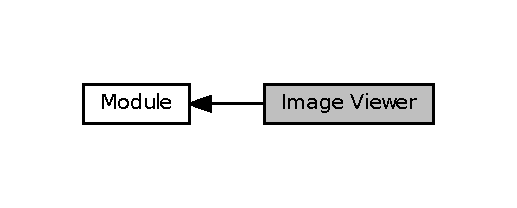
\includegraphics[width=248pt]{group__MODULE__IMAGE__VIEWER}
\end{center}
\end{figure}
\subsection*{Image Viewer Module}
\label{_amgrpfad8b2c2d595abc0721d685d1c68c286}%
Description of Display Module Init and Uninit funtions. \begin{DoxyCompactItemize}
\item 
\hyperlink{group__SYSTEM__ERROR_ga4540713b9a7a18ce44d78c3a10f7442f}{S\+N\+\_\+\+S\+T\+A\+T\+US} \hyperlink{group__MODULE__IMAGE__VIEWER_gafd26cb5c7532488dc8e0c37f07d16092}{S\+N\+\_\+\+M\+O\+D\+U\+L\+E\+\_\+\+I\+M\+A\+G\+E\+\_\+\+V\+I\+E\+W\+E\+R\+\_\+\+Init} (void)
\item 
\hyperlink{group__SYSTEM__ERROR_ga4540713b9a7a18ce44d78c3a10f7442f}{S\+N\+\_\+\+S\+T\+A\+T\+US} \hyperlink{group__MODULE__IMAGE__VIEWER_gae8357323213bf36b0a0011974f7c43dc}{S\+N\+\_\+\+M\+O\+D\+U\+L\+E\+\_\+\+I\+M\+A\+G\+E\+\_\+\+V\+I\+E\+W\+E\+R\+\_\+\+Destroy} (void)
\end{DoxyCompactItemize}
\subsection*{Image Viewer Module \+:\+: Printing}
\begin{DoxyCompactItemize}
\item 
\hyperlink{group__SYSTEM__ERROR_ga4540713b9a7a18ce44d78c3a10f7442f}{S\+N\+\_\+\+S\+T\+A\+T\+US} \hyperlink{group__MODULE__IMAGE__VIEWER_ga16b58f3bf4681b8ccda18d88490456a7}{S\+N\+\_\+\+M\+O\+D\+U\+L\+E\+\_\+\+I\+M\+A\+G\+E\+\_\+\+V\+I\+E\+W\+E\+R\+\_\+\+U\+P\+D\+A\+TE} (uint32\+\_\+t slice\+Index)
\end{DoxyCompactItemize}
\subsection*{Image Viewer Module \+:\+: Screen Control}
\begin{DoxyCompactItemize}
\item 
\hyperlink{group__SYSTEM__ERROR_ga4540713b9a7a18ce44d78c3a10f7442f}{S\+N\+\_\+\+S\+T\+A\+T\+US} \hyperlink{group__MODULE__IMAGE__VIEWER_ga77d2b7a49b61f4edf67ffc2466a032dd}{S\+N\+\_\+\+M\+O\+D\+U\+L\+E\+\_\+\+I\+M\+A\+G\+E\+\_\+\+V\+I\+E\+W\+E\+R\+\_\+\+C\+L\+E\+AR} (void)
\end{DoxyCompactItemize}


\subsection{Detailed Description}
Image Viewer Module Functions. 



\subsection{Function Documentation}
\mbox{\Hypertarget{group__MODULE__IMAGE__VIEWER_ga77d2b7a49b61f4edf67ffc2466a032dd}\label{group__MODULE__IMAGE__VIEWER_ga77d2b7a49b61f4edf67ffc2466a032dd}} 
\index{Image Viewer@{Image Viewer}!S\+N\+\_\+\+M\+O\+D\+U\+L\+E\+\_\+\+I\+M\+A\+G\+E\+\_\+\+V\+I\+E\+W\+E\+R\+\_\+\+C\+L\+E\+AR@{S\+N\+\_\+\+M\+O\+D\+U\+L\+E\+\_\+\+I\+M\+A\+G\+E\+\_\+\+V\+I\+E\+W\+E\+R\+\_\+\+C\+L\+E\+AR}}
\index{S\+N\+\_\+\+M\+O\+D\+U\+L\+E\+\_\+\+I\+M\+A\+G\+E\+\_\+\+V\+I\+E\+W\+E\+R\+\_\+\+C\+L\+E\+AR@{S\+N\+\_\+\+M\+O\+D\+U\+L\+E\+\_\+\+I\+M\+A\+G\+E\+\_\+\+V\+I\+E\+W\+E\+R\+\_\+\+C\+L\+E\+AR}!Image Viewer@{Image Viewer}}
\subsubsection{\texorpdfstring{S\+N\+\_\+\+M\+O\+D\+U\+L\+E\+\_\+\+I\+M\+A\+G\+E\+\_\+\+V\+I\+E\+W\+E\+R\+\_\+\+C\+L\+E\+A\+R()}{SN\_MODULE\_IMAGE\_VIEWER\_CLEAR()}}
{\footnotesize\ttfamily \hyperlink{group__SYSTEM__ERROR_ga4540713b9a7a18ce44d78c3a10f7442f}{S\+N\+\_\+\+S\+T\+A\+T\+US} S\+N\+\_\+\+M\+O\+D\+U\+L\+E\+\_\+\+I\+M\+A\+G\+E\+\_\+\+V\+I\+E\+W\+E\+R\+\_\+\+C\+L\+E\+AR (\begin{DoxyParamCaption}\item[{void}]{ }\end{DoxyParamCaption})}



{\ttfamily \#include $<$\hyperlink{SN__MODULE__IMAGE__VIEWER_8h}{M\+O\+D\+U\+L\+E/\+I\+N\+C\+L\+U\+D\+E/\+S\+N\+\_\+\+M\+O\+D\+U\+L\+E\+\_\+\+I\+M\+A\+G\+E\+\_\+\+V\+I\+E\+W\+E\+R.\+h}$>$}

\begin{DoxyReturn}{Returns}
S\+N\+\_\+\+S\+T\+A\+T\+US 
\end{DoxyReturn}
\begin{DoxyNote}{Note}

\end{DoxyNote}
\mbox{\Hypertarget{group__MODULE__IMAGE__VIEWER_gae8357323213bf36b0a0011974f7c43dc}\label{group__MODULE__IMAGE__VIEWER_gae8357323213bf36b0a0011974f7c43dc}} 
\index{Image Viewer@{Image Viewer}!S\+N\+\_\+\+M\+O\+D\+U\+L\+E\+\_\+\+I\+M\+A\+G\+E\+\_\+\+V\+I\+E\+W\+E\+R\+\_\+\+Destroy@{S\+N\+\_\+\+M\+O\+D\+U\+L\+E\+\_\+\+I\+M\+A\+G\+E\+\_\+\+V\+I\+E\+W\+E\+R\+\_\+\+Destroy}}
\index{S\+N\+\_\+\+M\+O\+D\+U\+L\+E\+\_\+\+I\+M\+A\+G\+E\+\_\+\+V\+I\+E\+W\+E\+R\+\_\+\+Destroy@{S\+N\+\_\+\+M\+O\+D\+U\+L\+E\+\_\+\+I\+M\+A\+G\+E\+\_\+\+V\+I\+E\+W\+E\+R\+\_\+\+Destroy}!Image Viewer@{Image Viewer}}
\subsubsection{\texorpdfstring{S\+N\+\_\+\+M\+O\+D\+U\+L\+E\+\_\+\+I\+M\+A\+G\+E\+\_\+\+V\+I\+E\+W\+E\+R\+\_\+\+Destroy()}{SN\_MODULE\_IMAGE\_VIEWER\_Destroy()}}
{\footnotesize\ttfamily \hyperlink{group__SYSTEM__ERROR_ga4540713b9a7a18ce44d78c3a10f7442f}{S\+N\+\_\+\+S\+T\+A\+T\+US} S\+N\+\_\+\+M\+O\+D\+U\+L\+E\+\_\+\+I\+M\+A\+G\+E\+\_\+\+V\+I\+E\+W\+E\+R\+\_\+\+Destroy (\begin{DoxyParamCaption}\item[{void}]{ }\end{DoxyParamCaption})}



{\ttfamily \#include $<$\hyperlink{SN__MODULE__IMAGE__VIEWER_8h}{M\+O\+D\+U\+L\+E/\+I\+N\+C\+L\+U\+D\+E/\+S\+N\+\_\+\+M\+O\+D\+U\+L\+E\+\_\+\+I\+M\+A\+G\+E\+\_\+\+V\+I\+E\+W\+E\+R.\+h}$>$}

\begin{DoxyReturn}{Returns}
S\+N\+\_\+\+S\+T\+A\+T\+US 
\end{DoxyReturn}
\begin{DoxyNote}{Note}

\end{DoxyNote}
\mbox{\Hypertarget{group__MODULE__IMAGE__VIEWER_gafd26cb5c7532488dc8e0c37f07d16092}\label{group__MODULE__IMAGE__VIEWER_gafd26cb5c7532488dc8e0c37f07d16092}} 
\index{Image Viewer@{Image Viewer}!S\+N\+\_\+\+M\+O\+D\+U\+L\+E\+\_\+\+I\+M\+A\+G\+E\+\_\+\+V\+I\+E\+W\+E\+R\+\_\+\+Init@{S\+N\+\_\+\+M\+O\+D\+U\+L\+E\+\_\+\+I\+M\+A\+G\+E\+\_\+\+V\+I\+E\+W\+E\+R\+\_\+\+Init}}
\index{S\+N\+\_\+\+M\+O\+D\+U\+L\+E\+\_\+\+I\+M\+A\+G\+E\+\_\+\+V\+I\+E\+W\+E\+R\+\_\+\+Init@{S\+N\+\_\+\+M\+O\+D\+U\+L\+E\+\_\+\+I\+M\+A\+G\+E\+\_\+\+V\+I\+E\+W\+E\+R\+\_\+\+Init}!Image Viewer@{Image Viewer}}
\subsubsection{\texorpdfstring{S\+N\+\_\+\+M\+O\+D\+U\+L\+E\+\_\+\+I\+M\+A\+G\+E\+\_\+\+V\+I\+E\+W\+E\+R\+\_\+\+Init()}{SN\_MODULE\_IMAGE\_VIEWER\_Init()}}
{\footnotesize\ttfamily \hyperlink{group__SYSTEM__ERROR_ga4540713b9a7a18ce44d78c3a10f7442f}{S\+N\+\_\+\+S\+T\+A\+T\+US} S\+N\+\_\+\+M\+O\+D\+U\+L\+E\+\_\+\+I\+M\+A\+G\+E\+\_\+\+V\+I\+E\+W\+E\+R\+\_\+\+Init (\begin{DoxyParamCaption}\item[{void}]{ }\end{DoxyParamCaption})}



{\ttfamily \#include $<$\hyperlink{SN__MODULE__IMAGE__VIEWER_8h}{M\+O\+D\+U\+L\+E/\+I\+N\+C\+L\+U\+D\+E/\+S\+N\+\_\+\+M\+O\+D\+U\+L\+E\+\_\+\+I\+M\+A\+G\+E\+\_\+\+V\+I\+E\+W\+E\+R.\+h}$>$}

\begin{DoxyReturn}{Returns}
S\+N\+\_\+\+S\+T\+A\+T\+US 
\end{DoxyReturn}
\begin{DoxyNote}{Note}

\end{DoxyNote}
\mbox{\Hypertarget{group__MODULE__IMAGE__VIEWER_ga16b58f3bf4681b8ccda18d88490456a7}\label{group__MODULE__IMAGE__VIEWER_ga16b58f3bf4681b8ccda18d88490456a7}} 
\index{Image Viewer@{Image Viewer}!S\+N\+\_\+\+M\+O\+D\+U\+L\+E\+\_\+\+I\+M\+A\+G\+E\+\_\+\+V\+I\+E\+W\+E\+R\+\_\+\+U\+P\+D\+A\+TE@{S\+N\+\_\+\+M\+O\+D\+U\+L\+E\+\_\+\+I\+M\+A\+G\+E\+\_\+\+V\+I\+E\+W\+E\+R\+\_\+\+U\+P\+D\+A\+TE}}
\index{S\+N\+\_\+\+M\+O\+D\+U\+L\+E\+\_\+\+I\+M\+A\+G\+E\+\_\+\+V\+I\+E\+W\+E\+R\+\_\+\+U\+P\+D\+A\+TE@{S\+N\+\_\+\+M\+O\+D\+U\+L\+E\+\_\+\+I\+M\+A\+G\+E\+\_\+\+V\+I\+E\+W\+E\+R\+\_\+\+U\+P\+D\+A\+TE}!Image Viewer@{Image Viewer}}
\subsubsection{\texorpdfstring{S\+N\+\_\+\+M\+O\+D\+U\+L\+E\+\_\+\+I\+M\+A\+G\+E\+\_\+\+V\+I\+E\+W\+E\+R\+\_\+\+U\+P\+D\+A\+T\+E()}{SN\_MODULE\_IMAGE\_VIEWER\_UPDATE()}}
{\footnotesize\ttfamily \hyperlink{group__SYSTEM__ERROR_ga4540713b9a7a18ce44d78c3a10f7442f}{S\+N\+\_\+\+S\+T\+A\+T\+US} S\+N\+\_\+\+M\+O\+D\+U\+L\+E\+\_\+\+I\+M\+A\+G\+E\+\_\+\+V\+I\+E\+W\+E\+R\+\_\+\+U\+P\+D\+A\+TE (\begin{DoxyParamCaption}\item[{uint32\+\_\+t}]{slice\+Index }\end{DoxyParamCaption})}



{\ttfamily \#include $<$\hyperlink{SN__MODULE__IMAGE__VIEWER_8h}{M\+O\+D\+U\+L\+E/\+I\+N\+C\+L\+U\+D\+E/\+S\+N\+\_\+\+M\+O\+D\+U\+L\+E\+\_\+\+I\+M\+A\+G\+E\+\_\+\+V\+I\+E\+W\+E\+R.\+h}$>$}


\begin{DoxyParams}{Parameters}
{\em slice\+Index} & \\
\hline
\end{DoxyParams}
\begin{DoxyReturn}{Returns}
S\+N\+\_\+\+S\+T\+A\+T\+US 
\end{DoxyReturn}
\begin{DoxyNote}{Note}

\end{DoxyNote}


���}	� �
����DEV��INO��SYN��SV~�#`F�#`F��#`F�k��u4I]�[s

���}	� �
����DEV��INO��SYN��SV~�#`S�#`SÀ#`S�k��v4I]�[s

���}	� �
����DEV��INO��SYN��SV~�#`[;#`[;�#`[;k���=I]�[s
\chapter{Class Documentation}

���}	� �
����DEV��INO��SYN��SV~�#`�#`ր#`�k��I]�[oB

���}	� �
����DEV��INO��SYN��SV~�#`�#`ր#`�k���I]�[o]

���}	� �
����DEV��INO��SYN��SV~�#`�#`ր#`�k���I]�[o
\hypertarget{structfile__system__page}{}\section{file\+\_\+system\+\_\+page Struct Reference}
\label{structfile__system__page}\index{file\+\_\+system\+\_\+page@{file\+\_\+system\+\_\+page}}


Collaboration diagram for file\+\_\+system\+\_\+page\+:\nopagebreak
\begin{figure}[H]
\begin{center}
\leavevmode
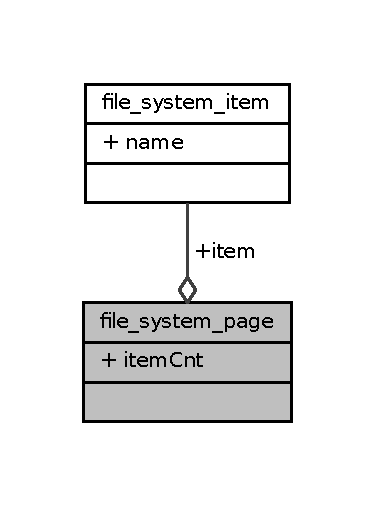
\includegraphics[width=180pt]{structfile__system__page__coll__graph}
\end{center}
\end{figure}
\subsection*{Public Attributes}
\begin{DoxyCompactItemize}
\item 
\mbox{\Hypertarget{structfile__system__page_a0cead090454a32e1bcdc14860d3a41bb}\label{structfile__system__page_a0cead090454a32e1bcdc14860d3a41bb}} 
\hyperlink{structfile__system__item}{fs\+Item\+\_\+t} {\bfseries item} \mbox{[}M\+A\+X\+\_\+\+I\+T\+E\+M\+\_\+\+S\+I\+ZE\mbox{]}
\item 
\mbox{\Hypertarget{structfile__system__page_ad586bea599d55aa2a410dee9feee20f9}\label{structfile__system__page_ad586bea599d55aa2a410dee9feee20f9}} 
uint32\+\_\+t {\bfseries item\+Cnt}
\end{DoxyCompactItemize}


The documentation for this struct was generated from the following file\+:\begin{DoxyCompactItemize}
\item 
M\+O\+D\+U\+L\+E/\+I\+N\+C\+L\+U\+D\+E/\hyperlink{SN__MODULE__FILE__SYSTEM_8h}{S\+N\+\_\+\+M\+O\+D\+U\+L\+E\+\_\+\+F\+I\+L\+E\+\_\+\+S\+Y\+S\+T\+E\+M.\+h}\end{DoxyCompactItemize}

\hypertarget{structfile__system__target}{}\section{file\+\_\+system\+\_\+target Struct Reference}
\label{structfile__system__target}\index{file\+\_\+system\+\_\+target@{file\+\_\+system\+\_\+target}}


Collaboration diagram for file\+\_\+system\+\_\+target\+:\nopagebreak
\begin{figure}[H]
\begin{center}
\leavevmode
\includegraphics[width=185pt]{structfile__system__target__coll__graph}
\end{center}
\end{figure}
\subsection*{Public Attributes}
\begin{DoxyCompactItemize}
\item 
\mbox{\Hypertarget{structfile__system__target_a6c7e2779e84950d492c24e4a0b46293d}\label{structfile__system__target_a6c7e2779e84950d492c24e4a0b46293d}} 
uint32\+\_\+t {\bfseries item\+\_\+index}
\item 
\mbox{\Hypertarget{structfile__system__target_ace1ec0d670b0e1956bb2de800f542d88}\label{structfile__system__target_ace1ec0d670b0e1956bb2de800f542d88}} 
uint32\+\_\+t {\bfseries page\+\_\+index}
\end{DoxyCompactItemize}


The documentation for this struct was generated from the following file\+:\begin{DoxyCompactItemize}
\item 
M\+O\+D\+U\+L\+E/\+I\+N\+C\+L\+U\+D\+E/\hyperlink{SN__MODULE__FILE__SYSTEM_8h}{S\+N\+\_\+\+M\+O\+D\+U\+L\+E\+\_\+\+F\+I\+L\+E\+\_\+\+S\+Y\+S\+T\+E\+M.\+h}\end{DoxyCompactItemize}


���}	� �
����DEV��INO��SYN��SV~�#`�#`ր#`�k���I]�[oG
\hypertarget{structgeneral__evt__t}{}\section{general\+\_\+evt\+\_\+t Struct Reference}
\label{structgeneral__evt__t}\index{general\+\_\+evt\+\_\+t@{general\+\_\+evt\+\_\+t}}


Collaboration diagram for general\+\_\+evt\+\_\+t\+:\nopagebreak
\begin{figure}[H]
\begin{center}
\leavevmode
\includegraphics[width=162pt]{structgeneral__evt__t__coll__graph}
\end{center}
\end{figure}
\subsection*{Public Attributes}
\begin{DoxyCompactItemize}
\item 
\mbox{\Hypertarget{structgeneral__evt__t_a2641588ad4dab3adfd0369a7afea080e}\label{structgeneral__evt__t_a2641588ad4dab3adfd0369a7afea080e}} 
event\+\_\+id\+\_\+t {\bfseries evt\+\_\+id}
\item 
\mbox{\Hypertarget{structgeneral__evt__t_a165ec408f6e8af4f7f4f9d9bbe2e5183}\label{structgeneral__evt__t_a165ec408f6e8af4f7f4f9d9bbe2e5183}} 
event\+\_\+msg\+\_\+t {\bfseries evt\+\_\+msg}
\end{DoxyCompactItemize}


The documentation for this struct was generated from the following file\+:\begin{DoxyCompactItemize}
\item 
S\+Y\+S\+T\+E\+M/\+I\+N\+C\+L\+U\+D\+E/\hyperlink{SN__SYS__MESSAGE__Q_8h}{S\+N\+\_\+\+S\+Y\+S\+\_\+\+M\+E\+S\+S\+A\+G\+E\+\_\+\+Q.\+h}\end{DoxyCompactItemize}

\hypertarget{structimage__viewer}{}\section{image\+\_\+viewer Struct Reference}
\label{structimage__viewer}\index{image\+\_\+viewer@{image\+\_\+viewer}}


Collaboration diagram for image\+\_\+viewer\+:\nopagebreak
\begin{figure}[H]
\begin{center}
\leavevmode
\includegraphics[width=350pt]{structimage__viewer__coll__graph}
\end{center}
\end{figure}
\subsection*{Public Attributes}
\begin{DoxyCompactItemize}
\item 
\mbox{\Hypertarget{structimage__viewer_a7aa8ff90430ce37f77e0473fef98acfb}\label{structimage__viewer_a7aa8ff90430ce37f77e0473fef98acfb}} 
S\+D\+L\+\_\+\+Window $\ast$ {\bfseries window}
\item 
\mbox{\Hypertarget{structimage__viewer_a15c11d0e9c16bb8cd2e66e533d29bf49}\label{structimage__viewer_a15c11d0e9c16bb8cd2e66e533d29bf49}} 
S\+D\+L\+\_\+\+Renderer $\ast$ {\bfseries renderer}
\item 
\mbox{\Hypertarget{structimage__viewer_abd3a6500c6dc389627ca4d88cb688d81}\label{structimage__viewer_abd3a6500c6dc389627ca4d88cb688d81}} 
S\+D\+L\+\_\+\+Texture $\ast$ {\bfseries texture}
\item 
\mbox{\Hypertarget{structimage__viewer_ab8b67fbf6967a2b072e7ceec0ad002c0}\label{structimage__viewer_ab8b67fbf6967a2b072e7ceec0ad002c0}} 
S\+D\+L\+\_\+\+Rect {\bfseries dest\+\_\+rect}
\item 
\mbox{\Hypertarget{structimage__viewer_ae34bb6294b7789eaaa37a917592d0a2c}\label{structimage__viewer_ae34bb6294b7789eaaa37a917592d0a2c}} 
\hyperlink{structmachine__information}{machine\+Info\+\_\+t} {\bfseries machine\+Info}
\item 
\mbox{\Hypertarget{structimage__viewer_a3f7d3425748942aaceb6dc66408d6355}\label{structimage__viewer_a3f7d3425748942aaceb6dc66408d6355}} 
\hyperlink{structprint__information}{print\+Info\+\_\+t} {\bfseries print\+Info}
\item 
\mbox{\Hypertarget{structimage__viewer_a39e8828eae966bbc9cf65e2a681ca9e7}\label{structimage__viewer_a39e8828eae966bbc9cf65e2a681ca9e7}} 
char $\ast$ {\bfseries image\+\_\+path}
\item 
\mbox{\Hypertarget{structimage__viewer_a55eb5d93ecd1e3a138d64b5d158980b0}\label{structimage__viewer_a55eb5d93ecd1e3a138d64b5d158980b0}} 
uint32\+\_\+t {\bfseries image\+\_\+w}
\item 
\mbox{\Hypertarget{structimage__viewer_aca799b98d1db4a741969dd24ecac358a}\label{structimage__viewer_aca799b98d1db4a741969dd24ecac358a}} 
uint32\+\_\+t {\bfseries image\+\_\+h}
\end{DoxyCompactItemize}


The documentation for this struct was generated from the following file\+:\begin{DoxyCompactItemize}
\item 
M\+O\+D\+U\+L\+E/\hyperlink{SN__MODULE__IMAGE__VIEWER_8c}{S\+N\+\_\+\+M\+O\+D\+U\+L\+E\+\_\+\+I\+M\+A\+G\+E\+\_\+\+V\+I\+E\+W\+E\+R.\+c}\end{DoxyCompactItemize}

\hypertarget{structmachine__information}{}\section{machine\+\_\+information Struct Reference}
\label{structmachine__information}\index{machine\+\_\+information@{machine\+\_\+information}}


Collaboration diagram for machine\+\_\+information\+:\nopagebreak
\begin{figure}[H]
\begin{center}
\leavevmode
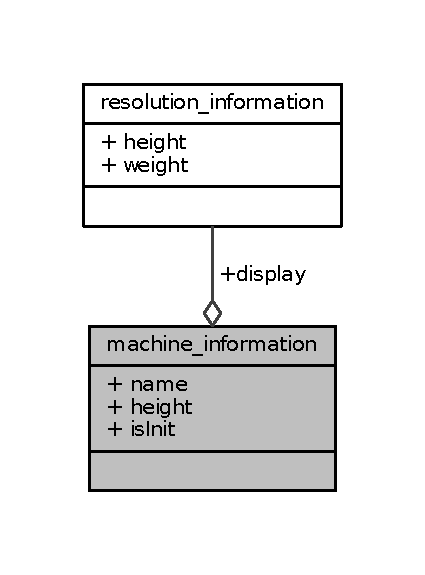
\includegraphics[width=204pt]{structmachine__information__coll__graph}
\end{center}
\end{figure}
\subsection*{Public Attributes}
\begin{DoxyCompactItemize}
\item 
\mbox{\Hypertarget{structmachine__information_ab98ac9579a14ca6351a586f6fe71aa7d}\label{structmachine__information_ab98ac9579a14ca6351a586f6fe71aa7d}} 
char {\bfseries name} \mbox{[}M\+A\+X\+\_\+\+F\+I\+L\+E\+N\+A\+M\+E\+\_\+\+L\+E\+N\+G\+TH\mbox{]}
\item 
\mbox{\Hypertarget{structmachine__information_afefc7bdff98f1d03477ac6f4175c65be}\label{structmachine__information_afefc7bdff98f1d03477ac6f4175c65be}} 
char {\bfseries height}
\item 
\mbox{\Hypertarget{structmachine__information_a8bba79e68a84d4f574247a1b069cb76b}\label{structmachine__information_a8bba79e68a84d4f574247a1b069cb76b}} 
\hyperlink{structresolution__information}{resolution\+\_\+t} {\bfseries display}
\item 
\mbox{\Hypertarget{structmachine__information_a2e4f3a82636bc57169cc5fcd3e9266ab}\label{structmachine__information_a2e4f3a82636bc57169cc5fcd3e9266ab}} 
bool {\bfseries is\+Init}
\end{DoxyCompactItemize}


The documentation for this struct was generated from the following file\+:\begin{DoxyCompactItemize}
\item 
M\+O\+D\+U\+L\+E/\+I\+N\+C\+L\+U\+D\+E/\hyperlink{SN__MODULE__FILE__SYSTEM_8h}{S\+N\+\_\+\+M\+O\+D\+U\+L\+E\+\_\+\+F\+I\+L\+E\+\_\+\+S\+Y\+S\+T\+E\+M.\+h}\end{DoxyCompactItemize}


���}	� �
����DEV��INO��SYN��SV~�#`�#`ր#`�k���I]�[oA

���}	� �
����DEV��INO��SYN��SV~�#`�#`ր#`�k���I]�[oC
\hypertarget{structmoduel__file__system}{}\section{moduel\+\_\+file\+\_\+system Struct Reference}
\label{structmoduel__file__system}\index{moduel\+\_\+file\+\_\+system@{moduel\+\_\+file\+\_\+system}}


Collaboration diagram for moduel\+\_\+file\+\_\+system\+:\nopagebreak
\begin{figure}[H]
\begin{center}
\leavevmode
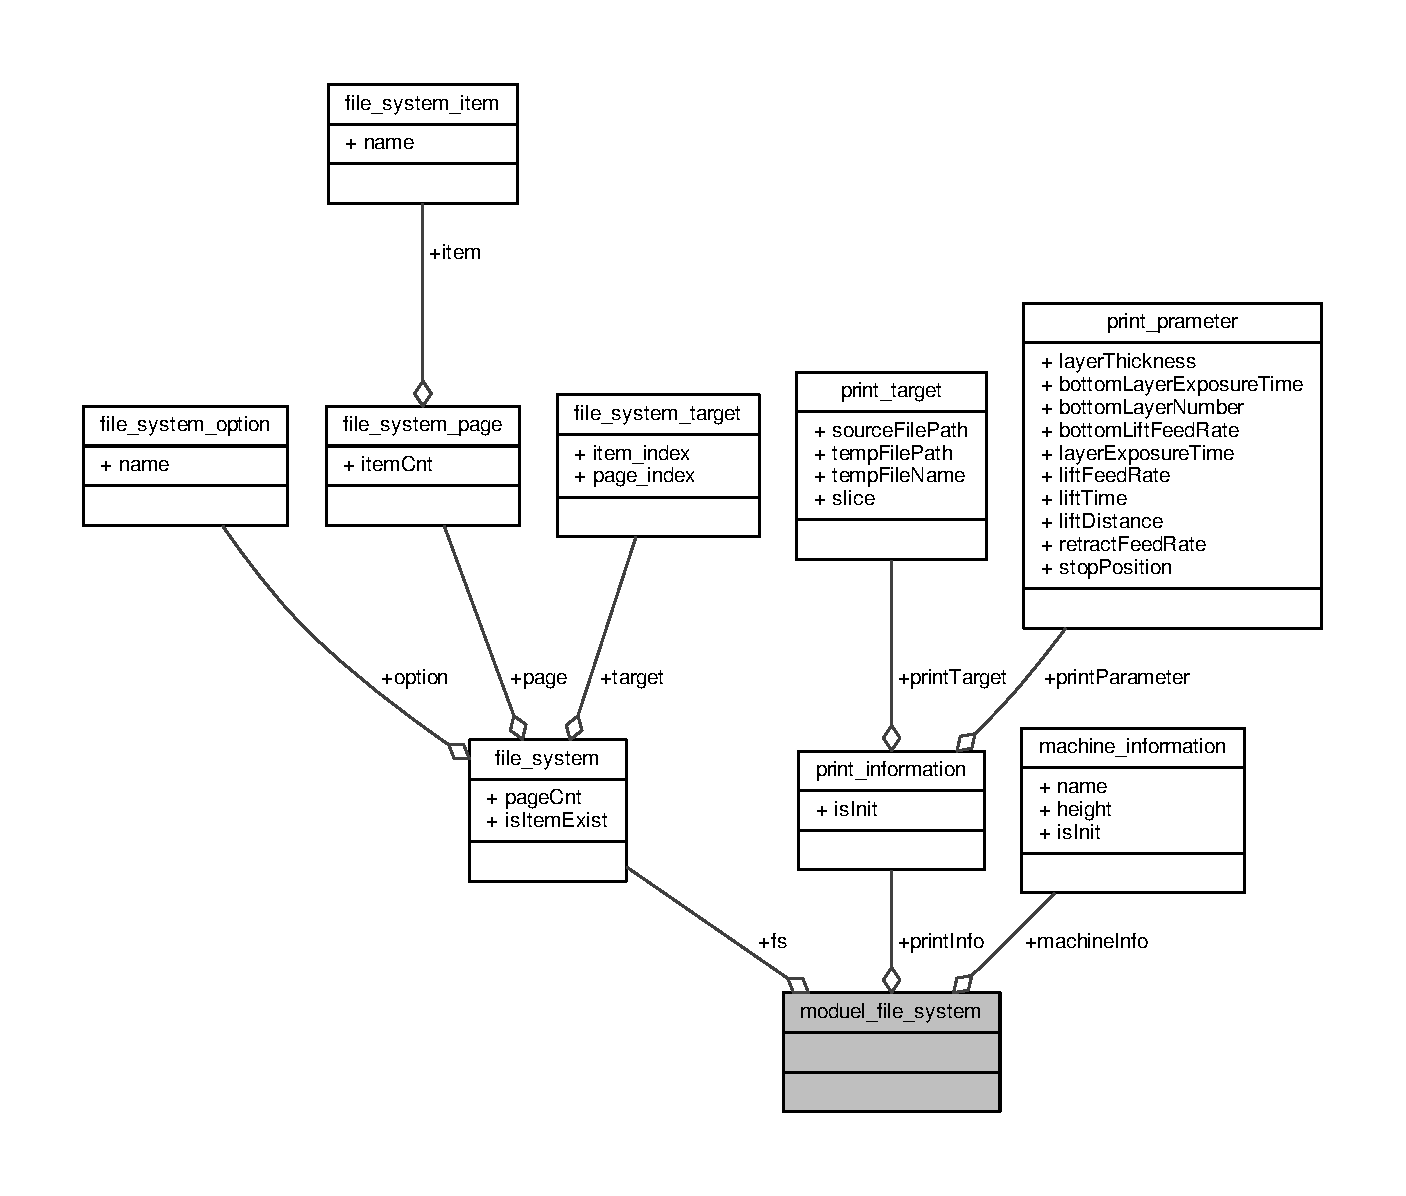
\includegraphics[width=350pt]{structmoduel__file__system__coll__graph}
\end{center}
\end{figure}
\subsection*{Public Attributes}
\begin{DoxyCompactItemize}
\item 
\mbox{\Hypertarget{structmoduel__file__system_aafdf8289cdfbf1c2f9b8d251a519e6bc}\label{structmoduel__file__system_aafdf8289cdfbf1c2f9b8d251a519e6bc}} 
\hyperlink{structfile__system}{fs\+\_\+t} {\bfseries fs}
\item 
\mbox{\Hypertarget{structmoduel__file__system_a764850bca89b06bf2e94119e2140c146}\label{structmoduel__file__system_a764850bca89b06bf2e94119e2140c146}} 
\hyperlink{structprint__information}{print\+Info\+\_\+t} {\bfseries print\+Info}
\item 
\mbox{\Hypertarget{structmoduel__file__system_a7f5988706364b1bb4b2110921b69c346}\label{structmoduel__file__system_a7f5988706364b1bb4b2110921b69c346}} 
\hyperlink{structmachine__information}{machine\+Info\+\_\+t} {\bfseries machine\+Info}
\end{DoxyCompactItemize}


The documentation for this struct was generated from the following file\+:\begin{DoxyCompactItemize}
\item 
M\+O\+D\+U\+L\+E/\hyperlink{SN__MODULE__FILE__SYSTEM_8c}{S\+N\+\_\+\+M\+O\+D\+U\+L\+E\+\_\+\+F\+I\+L\+E\+\_\+\+S\+Y\+S\+T\+E\+M.\+c}\end{DoxyCompactItemize}

\hypertarget{unionNextion__message}{}\section{Nextion\+\_\+message Union Reference}
\label{unionNextion__message}\index{Nextion\+\_\+message@{Nextion\+\_\+message}}


Collaboration diagram for Nextion\+\_\+message\+:\nopagebreak
\begin{figure}[H]
\begin{center}
\leavevmode
\includegraphics[width=184pt]{unionNextion__message__coll__graph}
\end{center}
\end{figure}
\subsection*{Public Attributes}
\begin{DoxyCompactItemize}
\item 
\mbox{\Hypertarget{unionNextion__message_a27222400844ea5f66aae9cedf02e896a}\label{unionNextion__message_a27222400844ea5f66aae9cedf02e896a}} 
\begin{tabbing}
xx\=xx\=xx\=xx\=xx\=xx\=xx\=xx\=xx\=\kill
struct \{\\
\>uint8\_t {\bfseries page}\\
\>uint8\_t {\bfseries type}\\
\>uint8\_t {\bfseries id}\\
\>uint8\_t {\bfseries value}\\
\>uint8\_t {\bfseries command}\\
\>uint8\_t {\bfseries endcode} \mbox{[}3\mbox{]}\\
\}; \\

\end{tabbing}\item 
\mbox{\Hypertarget{unionNextion__message_a4ae2d319d4a0b00ad495bfcc41478dc5}\label{unionNextion__message_a4ae2d319d4a0b00ad495bfcc41478dc5}} 
uint8\+\_\+t {\bfseries N\+Xmessage8bit} \mbox{[}8\mbox{]}
\item 
\mbox{\Hypertarget{unionNextion__message_a41e260dcf8e2c23d78a746433b1626e1}\label{unionNextion__message_a41e260dcf8e2c23d78a746433b1626e1}} 
uint32\+\_\+t {\bfseries N\+Xmessage} \mbox{[}2\mbox{]}
\end{DoxyCompactItemize}


The documentation for this union was generated from the following file\+:\begin{DoxyCompactItemize}
\item 
S\+Y\+S\+T\+E\+M/\+I\+N\+C\+L\+U\+D\+E/S\+N\+\_\+\+S\+Y\+S\+\_\+\+S\+E\+R\+I\+A\+L\+\_\+\+N\+E\+X\+T\+I\+O\+N.\+h\end{DoxyCompactItemize}


���}	� �
����DEV��INO��SYN��SV~�#`�#`ր#`�k���I]�[o<
\hypertarget{structprint__prameter}{}\section{print\+\_\+prameter Struct Reference}
\label{structprint__prameter}\index{print\+\_\+prameter@{print\+\_\+prameter}}


Collaboration diagram for print\+\_\+prameter\+:\nopagebreak
\begin{figure}[H]
\begin{center}
\leavevmode
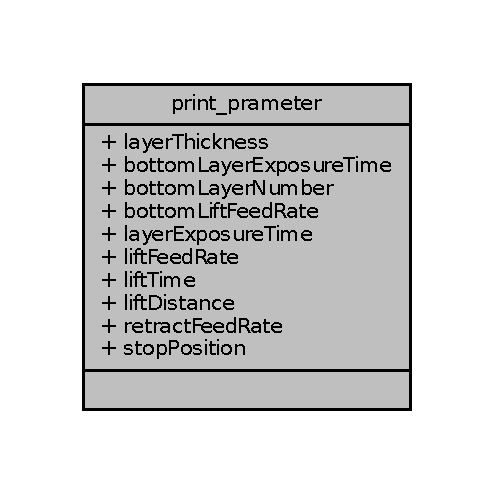
\includegraphics[width=237pt]{structprint__prameter__coll__graph}
\end{center}
\end{figure}
\subsection*{Public Attributes}
\begin{DoxyCompactItemize}
\item 
\mbox{\Hypertarget{structprint__prameter_abd09065a3d907abd26ddb981525ad35a}\label{structprint__prameter_abd09065a3d907abd26ddb981525ad35a}} 
float {\bfseries layer\+Thickness}
\item 
long \hyperlink{structprint__prameter_a4cad4458c035a54cbde08c36227bb82a}{bottom\+Layer\+Exposure\+Time}
\item 
\mbox{\Hypertarget{structprint__prameter_a2ea1a3922216a9d1fbdab1abfc37e5fa}\label{structprint__prameter_a2ea1a3922216a9d1fbdab1abfc37e5fa}} 
long {\bfseries bottom\+Layer\+Number}
\item 
\mbox{\Hypertarget{structprint__prameter_a87ad0abc66a28d11effc6e13dc3ca1a0}\label{structprint__prameter_a87ad0abc66a28d11effc6e13dc3ca1a0}} 
float {\bfseries bottom\+Lift\+Feed\+Rate}
\item 
long \hyperlink{structprint__prameter_a132ea30d7e46206117d917db4e2d1bcf}{layer\+Exposure\+Time}
\item 
\mbox{\Hypertarget{structprint__prameter_ab37375be2b8efeddf2d78316763f7523}\label{structprint__prameter_ab37375be2b8efeddf2d78316763f7523}} 
float {\bfseries lift\+Feed\+Rate}
\item 
\mbox{\Hypertarget{structprint__prameter_a8b69e9f209d8b1d9e2cfd175916a5717}\label{structprint__prameter_a8b69e9f209d8b1d9e2cfd175916a5717}} 
long {\bfseries lift\+Time}
\item 
\mbox{\Hypertarget{structprint__prameter_a70afbfab45c84387bf81d4f6e27bb825}\label{structprint__prameter_a70afbfab45c84387bf81d4f6e27bb825}} 
long {\bfseries lift\+Distance}
\item 
\mbox{\Hypertarget{structprint__prameter_a842278c540f5ec9784150c2ecff0472d}\label{structprint__prameter_a842278c540f5ec9784150c2ecff0472d}} 
float {\bfseries retract\+Feed\+Rate}
\item 
\mbox{\Hypertarget{structprint__prameter_a524cf4dd9639bafd6926d3fc2fe29071}\label{structprint__prameter_a524cf4dd9639bafd6926d3fc2fe29071}} 
float {\bfseries stop\+Position}
\end{DoxyCompactItemize}


\subsection{Member Data Documentation}
\mbox{\Hypertarget{structprint__prameter_a4cad4458c035a54cbde08c36227bb82a}\label{structprint__prameter_a4cad4458c035a54cbde08c36227bb82a}} 
\index{print\+\_\+prameter@{print\+\_\+prameter}!bottom\+Layer\+Exposure\+Time@{bottom\+Layer\+Exposure\+Time}}
\index{bottom\+Layer\+Exposure\+Time@{bottom\+Layer\+Exposure\+Time}!print\+\_\+prameter@{print\+\_\+prameter}}
\subsubsection{\texorpdfstring{bottom\+Layer\+Exposure\+Time}{bottomLayerExposureTime}}
{\footnotesize\ttfamily long print\+\_\+prameter\+::bottom\+Layer\+Exposure\+Time}

Bottom Layer Parameter \mbox{\Hypertarget{structprint__prameter_a132ea30d7e46206117d917db4e2d1bcf}\label{structprint__prameter_a132ea30d7e46206117d917db4e2d1bcf}} 
\index{print\+\_\+prameter@{print\+\_\+prameter}!layer\+Exposure\+Time@{layer\+Exposure\+Time}}
\index{layer\+Exposure\+Time@{layer\+Exposure\+Time}!print\+\_\+prameter@{print\+\_\+prameter}}
\subsubsection{\texorpdfstring{layer\+Exposure\+Time}{layerExposureTime}}
{\footnotesize\ttfamily long print\+\_\+prameter\+::layer\+Exposure\+Time}

Normal Layer Paramter 

The documentation for this struct was generated from the following file\+:\begin{DoxyCompactItemize}
\item 
M\+O\+D\+U\+L\+E/\+I\+N\+C\+L\+U\+D\+E/\hyperlink{SN__MODULE__FILE__SYSTEM_8h}{S\+N\+\_\+\+M\+O\+D\+U\+L\+E\+\_\+\+F\+I\+L\+E\+\_\+\+S\+Y\+S\+T\+E\+M.\+h}\end{DoxyCompactItemize}


���}	� �
����DEV��INO��SYN��SV~�#`�#`ր#`�k���I]�[o2

���}	� �
����DEV��INO��SYN��SV~�#`�#`ր#`�k���I]�[o

���}	� �
����DEV��INO��SYN��SV~�#`N#`N�#`Nk��h�I]�[wa
\hypertarget{structsys__serial__def}{}\section{sys\+\_\+serial\+\_\+def Struct Reference}
\label{structsys__serial__def}\index{sys\+\_\+serial\+\_\+def@{sys\+\_\+serial\+\_\+def}}


Collaboration diagram for sys\+\_\+serial\+\_\+def\+:\nopagebreak
\begin{figure}[H]
\begin{center}
\leavevmode
\includegraphics[width=163pt]{structsys__serial__def__coll__graph}
\end{center}
\end{figure}
\subsection*{Public Attributes}
\begin{DoxyCompactItemize}
\item 
\mbox{\Hypertarget{structsys__serial__def_a5a1f5b410efe38a5def8dffd93ebdd74}\label{structsys__serial__def_a5a1f5b410efe38a5def8dffd93ebdd74}} 
const char $\ast$ {\bfseries device}
\item 
\mbox{\Hypertarget{structsys__serial__def_aad2328bcf4fdbf9116207b0a7c91dbdc}\label{structsys__serial__def_aad2328bcf4fdbf9116207b0a7c91dbdc}} 
int {\bfseries oflags}
\item 
\mbox{\Hypertarget{structsys__serial__def_a8293f68f6d2c82c261e533de9171a52b}\label{structsys__serial__def_a8293f68f6d2c82c261e533de9171a52b}} 
int {\bfseries baud\+Rate}
\item 
\mbox{\Hypertarget{structsys__serial__def_a5ead55aa773aa1a067d5736dcc51329c}\label{structsys__serial__def_a5ead55aa773aa1a067d5736dcc51329c}} 
int {\bfseries rx\+Byte\+Size}
\item 
\mbox{\Hypertarget{structsys__serial__def_a53eb17eb80e427fb9f6777820629d490}\label{structsys__serial__def_a53eb17eb80e427fb9f6777820629d490}} 
int {\bfseries return\+Mode}
\item 
\mbox{\Hypertarget{structsys__serial__def_afecd2c4bce45b7815986cfbaa1d270c7}\label{structsys__serial__def_afecd2c4bce45b7815986cfbaa1d270c7}} 
char $\ast$ {\bfseries buffer}
\end{DoxyCompactItemize}


The documentation for this struct was generated from the following file\+:\begin{DoxyCompactItemize}
\item 
S\+Y\+S\+T\+E\+M/\+I\+N\+C\+L\+U\+D\+E/\hyperlink{SN__SYS__SERIAL__COMM_8h}{S\+N\+\_\+\+S\+Y\+S\+\_\+\+S\+E\+R\+I\+A\+L\+\_\+\+C\+O\+M\+M.\+h}\end{DoxyCompactItemize}

\hypertarget{structsys__serial__id}{}\section{sys\+\_\+serial\+\_\+id Struct Reference}
\label{structsys__serial__id}\index{sys\+\_\+serial\+\_\+id@{sys\+\_\+serial\+\_\+id}}


Collaboration diagram for sys\+\_\+serial\+\_\+id\+:\nopagebreak
\begin{figure}[H]
\begin{center}
\leavevmode
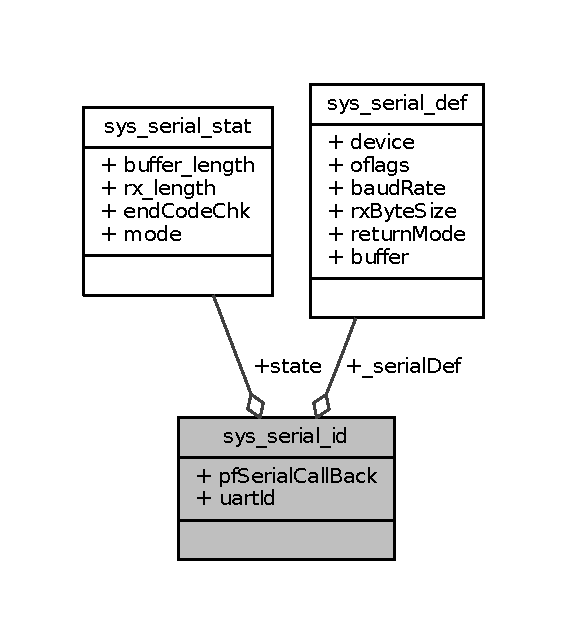
\includegraphics[width=272pt]{structsys__serial__id__coll__graph}
\end{center}
\end{figure}
\subsection*{Public Attributes}
\begin{DoxyCompactItemize}
\item 
\mbox{\Hypertarget{structsys__serial__id_a871517d57cdee8c3d17c79ff942d1590}\label{structsys__serial__id_a871517d57cdee8c3d17c79ff942d1590}} 
const \hyperlink{structsys__serial__def}{sys\+Serial\+Def\+\_\+t} $\ast$ {\bfseries \+\_\+serial\+Def}
\item 
\mbox{\Hypertarget{structsys__serial__id_a9f0d7f161757647b774e92b25fe02956}\label{structsys__serial__id_a9f0d7f161757647b774e92b25fe02956}} 
\hyperlink{structsys__serial__stat}{sys\+Serial\+Stat\+\_\+t} {\bfseries state}
\item 
\mbox{\Hypertarget{structsys__serial__id_a01e4caf41a2bb84168bdcd595d944dca}\label{structsys__serial__id_a01e4caf41a2bb84168bdcd595d944dca}} 
void $\ast$($\ast$ {\bfseries pf\+Serial\+Call\+Back} )(char $\ast$rx\+Buffer)
\item 
\mbox{\Hypertarget{structsys__serial__id_aac51b12503302e021b185a3310237b1e}\label{structsys__serial__id_aac51b12503302e021b185a3310237b1e}} 
uint32\+\_\+t {\bfseries uart\+Id}
\end{DoxyCompactItemize}


The documentation for this struct was generated from the following file\+:\begin{DoxyCompactItemize}
\item 
S\+Y\+S\+T\+E\+M/\+I\+N\+C\+L\+U\+D\+E/\hyperlink{SN__SYS__SERIAL__COMM_8h}{S\+N\+\_\+\+S\+Y\+S\+\_\+\+S\+E\+R\+I\+A\+L\+\_\+\+C\+O\+M\+M.\+h}\end{DoxyCompactItemize}

\hypertarget{structsys__serial__q}{}\section{sys\+\_\+serial\+\_\+q Struct Reference}
\label{structsys__serial__q}\index{sys\+\_\+serial\+\_\+q@{sys\+\_\+serial\+\_\+q}}


Collaboration diagram for sys\+\_\+serial\+\_\+q\+:\nopagebreak
\begin{figure}[H]
\begin{center}
\leavevmode
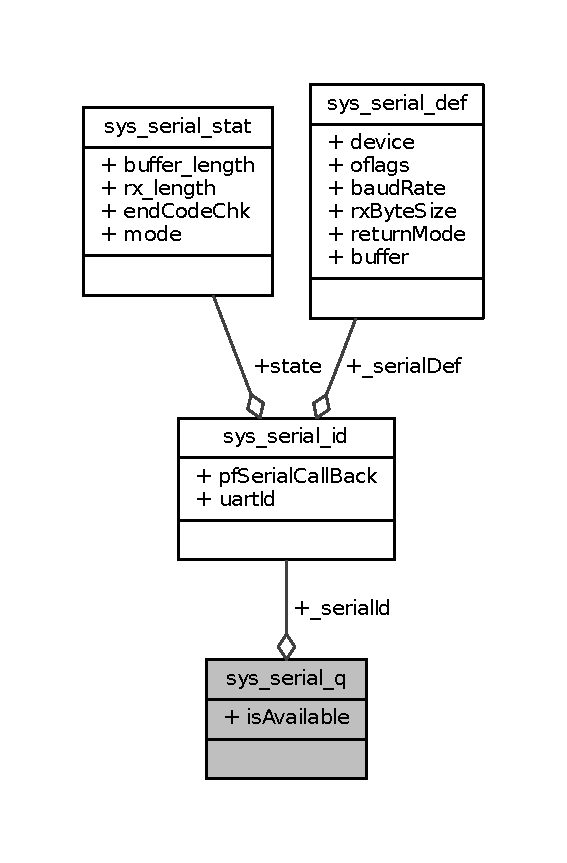
\includegraphics[width=272pt]{structsys__serial__q__coll__graph}
\end{center}
\end{figure}
\subsection*{Public Attributes}
\begin{DoxyCompactItemize}
\item 
\mbox{\Hypertarget{structsys__serial__q_a9609f82216c9986c4570496f3f8efe35}\label{structsys__serial__q_a9609f82216c9986c4570496f3f8efe35}} 
\hyperlink{structsys__serial__id}{sys\+Serial\+Id} {\bfseries \+\_\+serial\+Id}
\item 
\mbox{\Hypertarget{structsys__serial__q_ade2463824ded031f2aea3f5c7c3d0920}\label{structsys__serial__q_ade2463824ded031f2aea3f5c7c3d0920}} 
bool {\bfseries is\+Available}
\end{DoxyCompactItemize}


The documentation for this struct was generated from the following file\+:\begin{DoxyCompactItemize}
\item 
S\+Y\+S\+T\+E\+M/\+I\+N\+C\+L\+U\+D\+E/\hyperlink{SN__SYS__SERIAL__COMM_8h}{S\+N\+\_\+\+S\+Y\+S\+\_\+\+S\+E\+R\+I\+A\+L\+\_\+\+C\+O\+M\+M.\+h}\end{DoxyCompactItemize}


���}	� �
����DEV��INO��SYN��SV~�#`�#`ր#`�k���I]�[ol

���}	� �
����DEV��INO��SYN��SV~�#`�#`ր#`�k���I]�[o"

���}	� �
����DEV��INO��SYN��SV~�#`�#`ր#`�k���I]�[o=

���}	� �
����DEV��INO��SYN��SV~�#`�#`ր#`�k���I]�[o
\chapter{File Documentation}
\hypertarget{APPS_8h}{}\section{A\+P\+P/\+I\+N\+C\+L\+U\+D\+E/\+A\+P\+PS.h File Reference}
\label{APPS_8h}\index{A\+P\+P/\+I\+N\+C\+L\+U\+D\+E/\+A\+P\+P\+S.\+h@{A\+P\+P/\+I\+N\+C\+L\+U\+D\+E/\+A\+P\+P\+S.\+h}}
{\ttfamily \#include \char`\"{}S\+N\+\_\+\+A\+P\+I.\+h\char`\"{}}\newline
{\ttfamily \#include \char`\"{}A\+P\+P\+\_\+\+S\+T\+A\+T\+E.\+h\char`\"{}}\newline
{\ttfamily \#include \char`\"{}A\+P\+P\+\_\+\+M\+A\+I\+N.\+h\char`\"{}}\newline
{\ttfamily \#include \char`\"{}A\+P\+P\+\_\+\+F\+I\+L\+E\+\_\+\+S\+E\+L\+E\+C\+T.\+h\char`\"{}}\newline
{\ttfamily \#include \char`\"{}A\+P\+P\+\_\+\+P\+R\+I\+N\+T\+I\+N\+G.\+h\char`\"{}}\newline
{\ttfamily \#include \char`\"{}A\+P\+P\+\_\+\+W\+A\+I\+T\+I\+N\+G.\+h\char`\"{}}\newline
{\ttfamily \#include \char`\"{}A\+P\+P\+\_\+\+P\+A\+U\+S\+E.\+h\char`\"{}}\newline
{\ttfamily \#include \char`\"{}A\+P\+P\+\_\+\+C\+O\+N\+T\+R\+O\+L.\+h\char`\"{}}\newline
{\ttfamily \#include \char`\"{}A\+P\+P\+\_\+\+I\+N\+I\+T.\+h\char`\"{}}\newline
Include dependency graph for A\+P\+P\+S.\+h\+:
\nopagebreak
\begin{figure}[H]
\begin{center}
\leavevmode
\includegraphics[width=350pt]{APPS_8h__incl}
\end{center}
\end{figure}
This graph shows which files directly or indirectly include this file\+:
\nopagebreak
\begin{figure}[H]
\begin{center}
\leavevmode
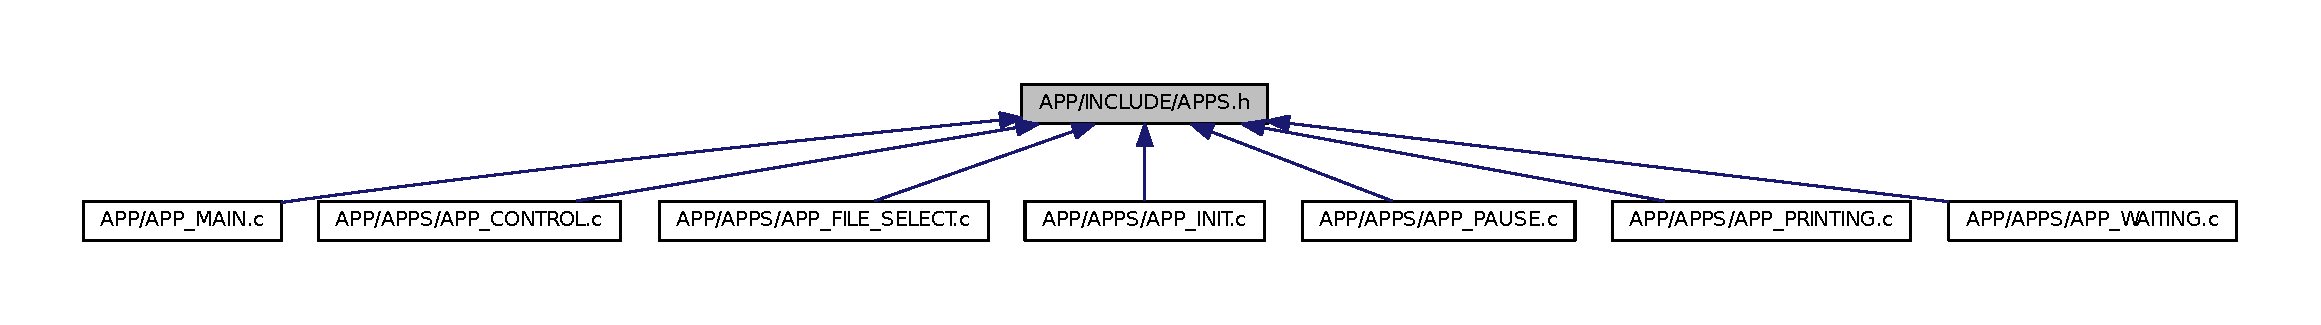
\includegraphics[width=350pt]{APPS_8h__dep__incl}
\end{center}
\end{figure}


\subsection{Detailed Description}
\begin{DoxyAuthor}{Author}
Bato 
\end{DoxyAuthor}
\begin{DoxyDate}{Date}
1 Oct 2018 
\end{DoxyDate}
\begin{DoxySeeAlso}{See also}
\href{http://www.stack.nl/~dimitri/doxygen/docblocks.html}{\tt http\+://www.\+stack.\+nl/$\sim$dimitri/doxygen/docblocks.\+html} 

\href{http://www.stack.nl/~dimitri/doxygen/commands.html}{\tt http\+://www.\+stack.\+nl/$\sim$dimitri/doxygen/commands.\+html} 
\end{DoxySeeAlso}

\hypertarget{SN__API_8h}{}\section{I\+N\+C\+L\+U\+D\+E/\+S\+N\+\_\+\+A\+PI.h File Reference}
\label{SN__API_8h}\index{I\+N\+C\+L\+U\+D\+E/\+S\+N\+\_\+\+A\+P\+I.\+h@{I\+N\+C\+L\+U\+D\+E/\+S\+N\+\_\+\+A\+P\+I.\+h}}
{\ttfamily \#include $<$stdio.\+h$>$}\newline
{\ttfamily \#include $<$stdlib.\+h$>$}\newline
{\ttfamily \#include $<$string.\+h$>$}\newline
{\ttfamily \#include $<$stdint.\+h$>$}\newline
{\ttfamily \#include $<$stdbool.\+h$>$}\newline
{\ttfamily \#include $<$fcntl.\+h$>$}\newline
{\ttfamily \#include $<$pthread.\+h$>$}\newline
{\ttfamily \#include $<$semaphore.\+h$>$}\newline
{\ttfamily \#include $<$signal.\+h$>$}\newline
{\ttfamily \#include $<$time.\+h$>$}\newline
{\ttfamily \#include $<$sys/types.\+h$>$}\newline
{\ttfamily \#include $<$sys/ipc.\+h$>$}\newline
{\ttfamily \#include $<$sys/msg.\+h$>$}\newline
{\ttfamily \#include $<$sys/stat.\+h$>$}\newline
{\ttfamily \#include $<$sys/poll.\+h$>$}\newline
{\ttfamily \#include $<$sys/time.\+h$>$}\newline
{\ttfamily \#include $<$sys/mman.\+h$>$}\newline
{\ttfamily \#include $<$sys/ioctl.\+h$>$}\newline
{\ttfamily \#include $<$errno.\+h$>$}\newline
{\ttfamily \#include $<$dirent.\+h$>$}\newline
{\ttfamily \#include $<$termios.\+h$>$}\newline
{\ttfamily \#include $<$unistd.\+h$>$}\newline
{\ttfamily \#include $<$zip.\+h$>$}\newline
{\ttfamily \#include \char`\"{}S\+N\+\_\+\+S\+Y\+S\+T\+E\+M.\+h\char`\"{}}\newline
{\ttfamily \#include \char`\"{}S\+N\+\_\+\+M\+O\+D\+U\+L\+E.\+h\char`\"{}}\newline
{\ttfamily \#include \char`\"{}A\+P\+P\+\_\+\+M\+E\+S\+S\+A\+G\+E\+S.\+h\char`\"{}}\newline
Include dependency graph for S\+N\+\_\+\+A\+P\+I.\+h\+:
\nopagebreak
\begin{figure}[H]
\begin{center}
\leavevmode
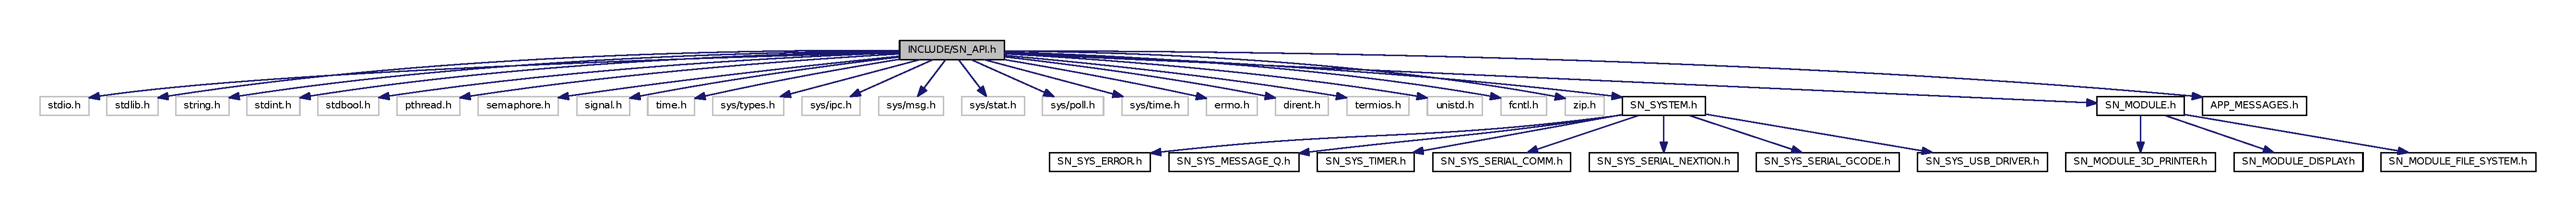
\includegraphics[width=350pt]{SN__API_8h__incl}
\end{center}
\end{figure}
This graph shows which files directly or indirectly include this file\+:
\nopagebreak
\begin{figure}[H]
\begin{center}
\leavevmode
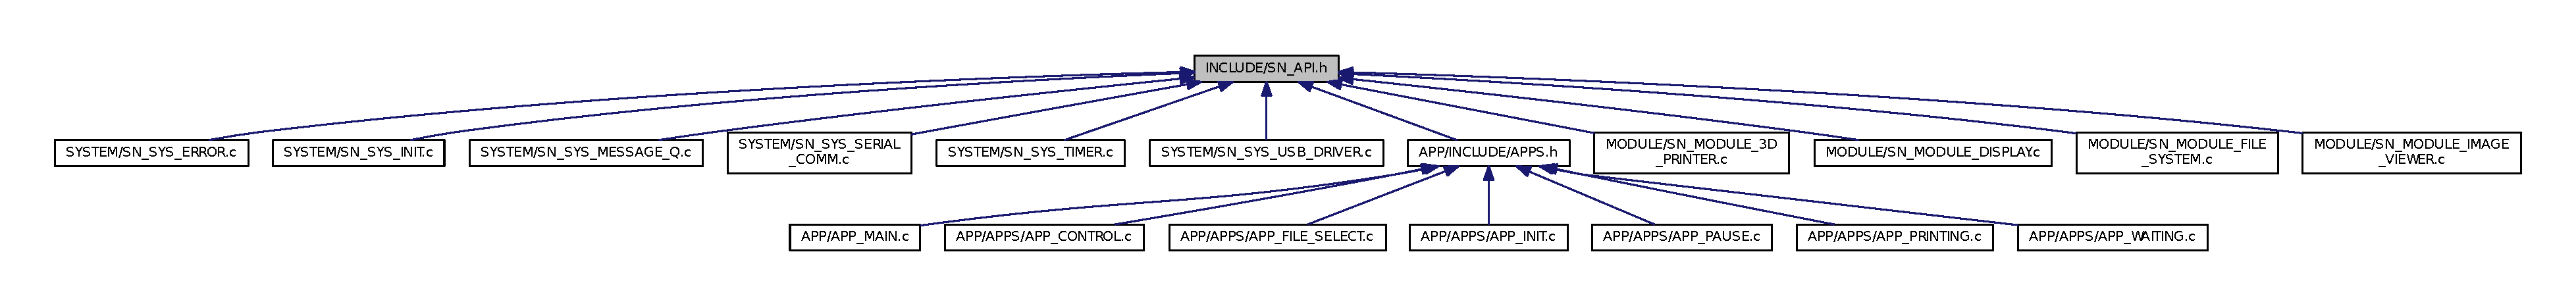
\includegraphics[width=350pt]{SN__API_8h__dep__incl}
\end{center}
\end{figure}
\subsection*{Macros}
\begin{DoxyCompactItemize}
\item 
\#define {\bfseries true}~1
\item 
\#define {\bfseries false}~0
\end{DoxyCompactItemize}
\subsection*{Typedefs}
\begin{DoxyCompactItemize}
\item 
typedef int {\bfseries bool}
\end{DoxyCompactItemize}


\subsection{Detailed Description}
\begin{DoxyAuthor}{Author}
Bato 
\end{DoxyAuthor}
\begin{DoxyDate}{Date}
18 Sep 2018 
\end{DoxyDate}
\begin{DoxySeeAlso}{See also}
\href{http://www.stack.nl/~dimitri/doxygen/docblocks.html}{\tt http\+://www.\+stack.\+nl/$\sim$dimitri/doxygen/docblocks.\+html} 

\href{http://www.stack.nl/~dimitri/doxygen/commands.html}{\tt http\+://www.\+stack.\+nl/$\sim$dimitri/doxygen/commands.\+html} 
\end{DoxySeeAlso}

\hypertarget{SN__MODULE_8h}{}\section{I\+N\+C\+L\+U\+D\+E/\+S\+N\+\_\+\+M\+O\+D\+U\+LE.h File Reference}
\label{SN__MODULE_8h}\index{I\+N\+C\+L\+U\+D\+E/\+S\+N\+\_\+\+M\+O\+D\+U\+L\+E.\+h@{I\+N\+C\+L\+U\+D\+E/\+S\+N\+\_\+\+M\+O\+D\+U\+L\+E.\+h}}
{\ttfamily \#include \char`\"{}S\+N\+\_\+\+M\+O\+D\+U\+L\+E\+\_\+3\+D\+\_\+\+P\+R\+I\+N\+T\+E\+R.\+h\char`\"{}}\newline
{\ttfamily \#include \char`\"{}S\+N\+\_\+\+M\+O\+D\+U\+L\+E\+\_\+\+D\+I\+S\+P\+L\+A\+Y.\+h\char`\"{}}\newline
{\ttfamily \#include \char`\"{}S\+N\+\_\+\+M\+O\+D\+U\+L\+E\+\_\+\+F\+I\+L\+E\+\_\+\+S\+Y\+S\+T\+E\+M.\+h\char`\"{}}\newline
Include dependency graph for S\+N\+\_\+\+M\+O\+D\+U\+L\+E.\+h\+:\nopagebreak
\begin{figure}[H]
\begin{center}
\leavevmode
\includegraphics[width=350pt]{SN__MODULE_8h__incl}
\end{center}
\end{figure}
This graph shows which files directly or indirectly include this file\+:
\nopagebreak
\begin{figure}[H]
\begin{center}
\leavevmode
\includegraphics[width=350pt]{SN__MODULE_8h__dep__incl}
\end{center}
\end{figure}


\subsection{Detailed Description}
\begin{DoxyAuthor}{Author}
Bato 
\end{DoxyAuthor}
\begin{DoxyDate}{Date}
1 Oct 2018 
\end{DoxyDate}
\begin{DoxySeeAlso}{See also}
\href{http://www.stack.nl/~dimitri/doxygen/docblocks.html}{\tt http\+://www.\+stack.\+nl/$\sim$dimitri/doxygen/docblocks.\+html} 

\href{http://www.stack.nl/~dimitri/doxygen/commands.html}{\tt http\+://www.\+stack.\+nl/$\sim$dimitri/doxygen/commands.\+html} 
\end{DoxySeeAlso}


���}	� �
����DEV��INO��SYN��SV~�#`(#`(�#`(k��H�I]�[~
\hypertarget{SN__MODULE__3D__PRINTER_8h}{}\section{M\+O\+D\+U\+L\+E/\+I\+N\+C\+L\+U\+D\+E/\+S\+N\+\_\+\+M\+O\+D\+U\+L\+E\+\_\+3\+D\+\_\+\+P\+R\+I\+N\+T\+ER.h File Reference}
\label{SN__MODULE__3D__PRINTER_8h}\index{M\+O\+D\+U\+L\+E/\+I\+N\+C\+L\+U\+D\+E/\+S\+N\+\_\+\+M\+O\+D\+U\+L\+E\+\_\+3\+D\+\_\+\+P\+R\+I\+N\+T\+E\+R.\+h@{M\+O\+D\+U\+L\+E/\+I\+N\+C\+L\+U\+D\+E/\+S\+N\+\_\+\+M\+O\+D\+U\+L\+E\+\_\+3\+D\+\_\+\+P\+R\+I\+N\+T\+E\+R.\+h}}
This graph shows which files directly or indirectly include this file\+:\nopagebreak
\begin{figure}[H]
\begin{center}
\leavevmode
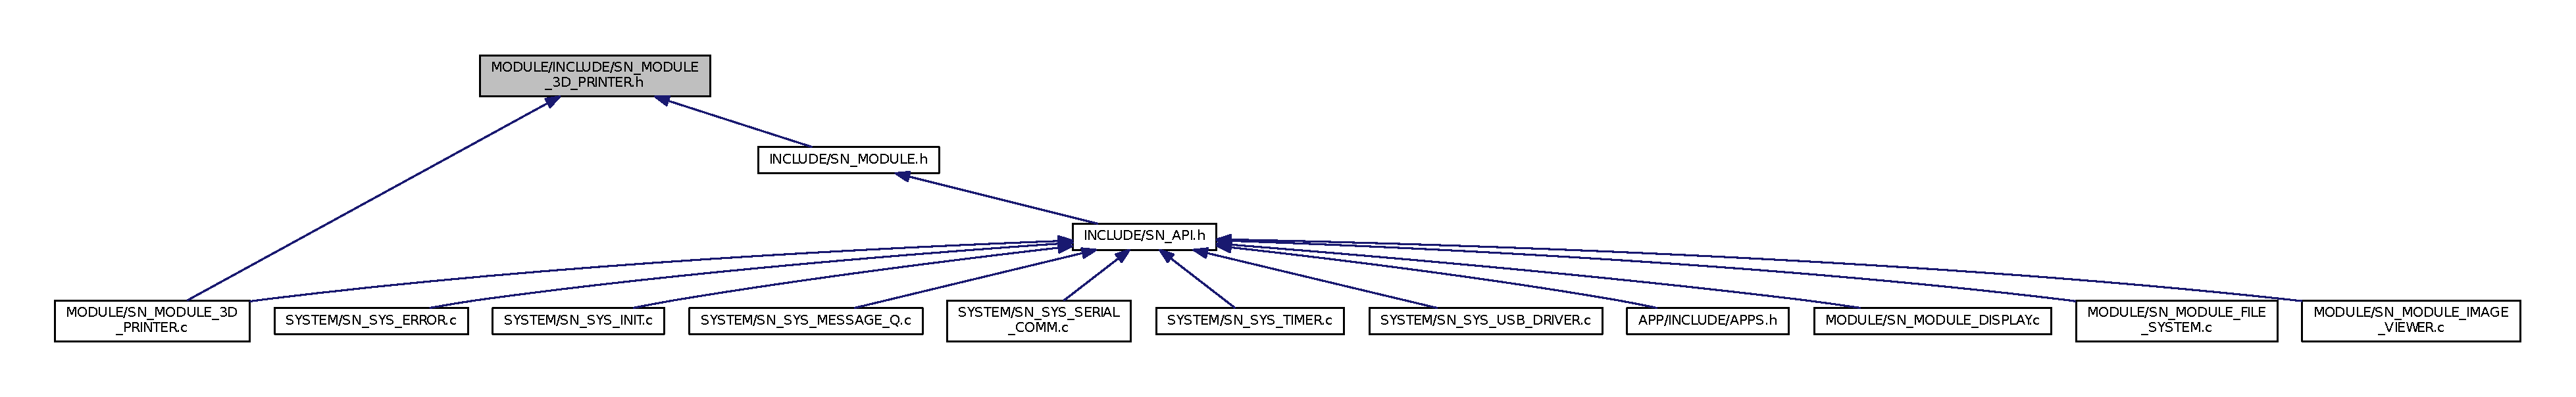
\includegraphics[width=350pt]{SN__MODULE__3D__PRINTER_8h__dep__incl}
\end{center}
\end{figure}
\subsection*{Functions}
\begin{DoxyCompactItemize}
\item 
\hyperlink{group__SYSTEM__ERROR_ga4540713b9a7a18ce44d78c3a10f7442f}{S\+N\+\_\+\+S\+T\+A\+T\+US} {\bfseries S\+N\+\_\+\+M\+O\+D\+U\+L\+E\+\_\+3\+D\+\_\+\+P\+R\+I\+N\+T\+E\+R\+\_\+\+Test} (void)
\end{DoxyCompactItemize}
\begin{Indent}\textbf{ 3D Printr Module}\par
{\em Description of 3D Printr Module Init and Uninit funtions. }\begin{DoxyCompactItemize}
\item 
\hyperlink{group__SYSTEM__ERROR_ga4540713b9a7a18ce44d78c3a10f7442f}{S\+N\+\_\+\+S\+T\+A\+T\+US} \hyperlink{group__MODULE__3D__PRINTER_ga801e265ffe6f8c56081112f4fdd35f39}{S\+N\+\_\+\+M\+O\+D\+U\+L\+E\+\_\+3\+D\+\_\+\+P\+R\+I\+N\+T\+E\+R\+\_\+\+Init} (void)
\item 
\hyperlink{group__SYSTEM__ERROR_ga4540713b9a7a18ce44d78c3a10f7442f}{S\+N\+\_\+\+S\+T\+A\+T\+US} \hyperlink{group__MODULE__3D__PRINTER_ga776f5e31b0c0e176e35669f9432baec0}{S\+N\+\_\+\+M\+O\+D\+U\+L\+E\+\_\+3\+D\+\_\+\+P\+R\+I\+N\+T\+E\+R\+\_\+\+Uninit} (void)
\end{DoxyCompactItemize}
\end{Indent}
\begin{Indent}\textbf{ 3D Printer Module \+:\+: Printing.}\par
{\em Description of 3D Printr Module funtions. }\begin{DoxyCompactItemize}
\item 
\hyperlink{group__SYSTEM__ERROR_ga4540713b9a7a18ce44d78c3a10f7442f}{S\+N\+\_\+\+S\+T\+A\+T\+US} \hyperlink{group__MODULE__3D__PRINTER_ga439ebb10f8ee839218655c5177e9110b}{S\+N\+\_\+\+M\+O\+D\+U\+L\+E\+\_\+3\+D\+\_\+\+P\+R\+I\+N\+T\+E\+R\+\_\+\+Start} (uint32\+\_\+t page\+Index, uint32\+\_\+t item\+Index)
\item 
\hyperlink{group__SYSTEM__ERROR_ga4540713b9a7a18ce44d78c3a10f7442f}{S\+N\+\_\+\+S\+T\+A\+T\+US} \hyperlink{group__MODULE__3D__PRINTER_ga21ca69a451fafe2c9218c9a1737e1f15}{S\+N\+\_\+\+M\+O\+D\+U\+L\+E\+\_\+3\+D\+\_\+\+P\+R\+I\+N\+T\+E\+R\+\_\+\+Stop} (void)
\item 
\hyperlink{group__SYSTEM__ERROR_ga4540713b9a7a18ce44d78c3a10f7442f}{S\+N\+\_\+\+S\+T\+A\+T\+US} \hyperlink{group__MODULE__3D__PRINTER_ga84a03238ddc0021011c12839757bf8c2}{S\+N\+\_\+\+M\+O\+D\+U\+L\+E\+\_\+3\+D\+\_\+\+P\+R\+I\+N\+T\+E\+R\+\_\+\+Pause} (void)
\item 
\hyperlink{group__SYSTEM__ERROR_ga4540713b9a7a18ce44d78c3a10f7442f}{S\+N\+\_\+\+S\+T\+A\+T\+US} \hyperlink{group__MODULE__3D__PRINTER_gaabec8b5f01119d989d725eff26053ca5}{S\+N\+\_\+\+M\+O\+D\+U\+L\+E\+\_\+3\+D\+\_\+\+P\+R\+I\+N\+T\+E\+R\+\_\+\+Resume} (void)
\end{DoxyCompactItemize}
\end{Indent}
\begin{Indent}\textbf{ 3D Printer Module \+:\+: Z Control.}\par
{\em Description of 3D Printr Module funtions. }\begin{DoxyCompactItemize}
\item 
\hyperlink{group__SYSTEM__ERROR_ga4540713b9a7a18ce44d78c3a10f7442f}{S\+N\+\_\+\+S\+T\+A\+T\+US} \hyperlink{group__MODULE__3D__PRINTER_ga83ec7a117b45a5760e1aecde26f69dea}{S\+N\+\_\+\+M\+O\+D\+U\+L\+E\+\_\+3\+D\+\_\+\+P\+R\+I\+N\+T\+E\+R\+\_\+\+Motor\+Init} (void)
\item 
\hyperlink{group__SYSTEM__ERROR_ga4540713b9a7a18ce44d78c3a10f7442f}{S\+N\+\_\+\+S\+T\+A\+T\+US} \hyperlink{group__MODULE__3D__PRINTER_ga2f644e451b310348d50fef6c762bbbcc}{S\+N\+\_\+\+M\+O\+D\+U\+L\+E\+\_\+3\+D\+\_\+\+P\+R\+I\+N\+T\+E\+R\+\_\+\+Motor\+Uninit} (void)
\item 
\hyperlink{group__SYSTEM__ERROR_ga4540713b9a7a18ce44d78c3a10f7442f}{S\+N\+\_\+\+S\+T\+A\+T\+US} \hyperlink{group__MODULE__3D__PRINTER_ga7bba4aa3966da87ac001b67b301310c1}{S\+N\+\_\+\+M\+O\+D\+U\+L\+E\+\_\+3\+D\+\_\+\+P\+R\+I\+N\+T\+E\+R\+\_\+\+Z\+\_\+\+Homing} (void)
\item 
\hyperlink{group__SYSTEM__ERROR_ga4540713b9a7a18ce44d78c3a10f7442f}{S\+N\+\_\+\+S\+T\+A\+T\+US} \hyperlink{group__MODULE__3D__PRINTER_ga47326e9f9d52dae584ee7c12011efc64}{S\+N\+\_\+\+M\+O\+D\+U\+L\+E\+\_\+3\+D\+\_\+\+P\+R\+I\+N\+T\+E\+R\+\_\+\+Z\+\_\+\+Up} (float mm)
\item 
\hyperlink{group__SYSTEM__ERROR_ga4540713b9a7a18ce44d78c3a10f7442f}{S\+N\+\_\+\+S\+T\+A\+T\+US} \hyperlink{group__MODULE__3D__PRINTER_ga65e82d5d94b534427c5d036080e77cf0}{S\+N\+\_\+\+M\+O\+D\+U\+L\+E\+\_\+3\+D\+\_\+\+P\+R\+I\+N\+T\+E\+R\+\_\+\+Z\+\_\+\+Down} (float mm)
\end{DoxyCompactItemize}
\end{Indent}


\subsection{Detailed Description}
\begin{DoxyAuthor}{Author}
Bato 
\end{DoxyAuthor}
\begin{DoxyDate}{Date}
18 Sep 2018 
\end{DoxyDate}
\begin{DoxySeeAlso}{See also}
\href{http://www.stack.nl/~dimitri/doxygen/docblocks.html}{\tt http\+://www.\+stack.\+nl/$\sim$dimitri/doxygen/docblocks.\+html} 

\href{http://www.stack.nl/~dimitri/doxygen/commands.html}{\tt http\+://www.\+stack.\+nl/$\sim$dimitri/doxygen/commands.\+html} 
\end{DoxySeeAlso}

\hypertarget{SN__MODULE__DISPLAY_8h}{}\section{M\+O\+D\+U\+L\+E/\+I\+N\+C\+L\+U\+D\+E/\+S\+N\+\_\+\+M\+O\+D\+U\+L\+E\+\_\+\+D\+I\+S\+P\+L\+AY.h File Reference}
\label{SN__MODULE__DISPLAY_8h}\index{M\+O\+D\+U\+L\+E/\+I\+N\+C\+L\+U\+D\+E/\+S\+N\+\_\+\+M\+O\+D\+U\+L\+E\+\_\+\+D\+I\+S\+P\+L\+A\+Y.\+h@{M\+O\+D\+U\+L\+E/\+I\+N\+C\+L\+U\+D\+E/\+S\+N\+\_\+\+M\+O\+D\+U\+L\+E\+\_\+\+D\+I\+S\+P\+L\+A\+Y.\+h}}
This graph shows which files directly or indirectly include this file\+:\nopagebreak
\begin{figure}[H]
\begin{center}
\leavevmode
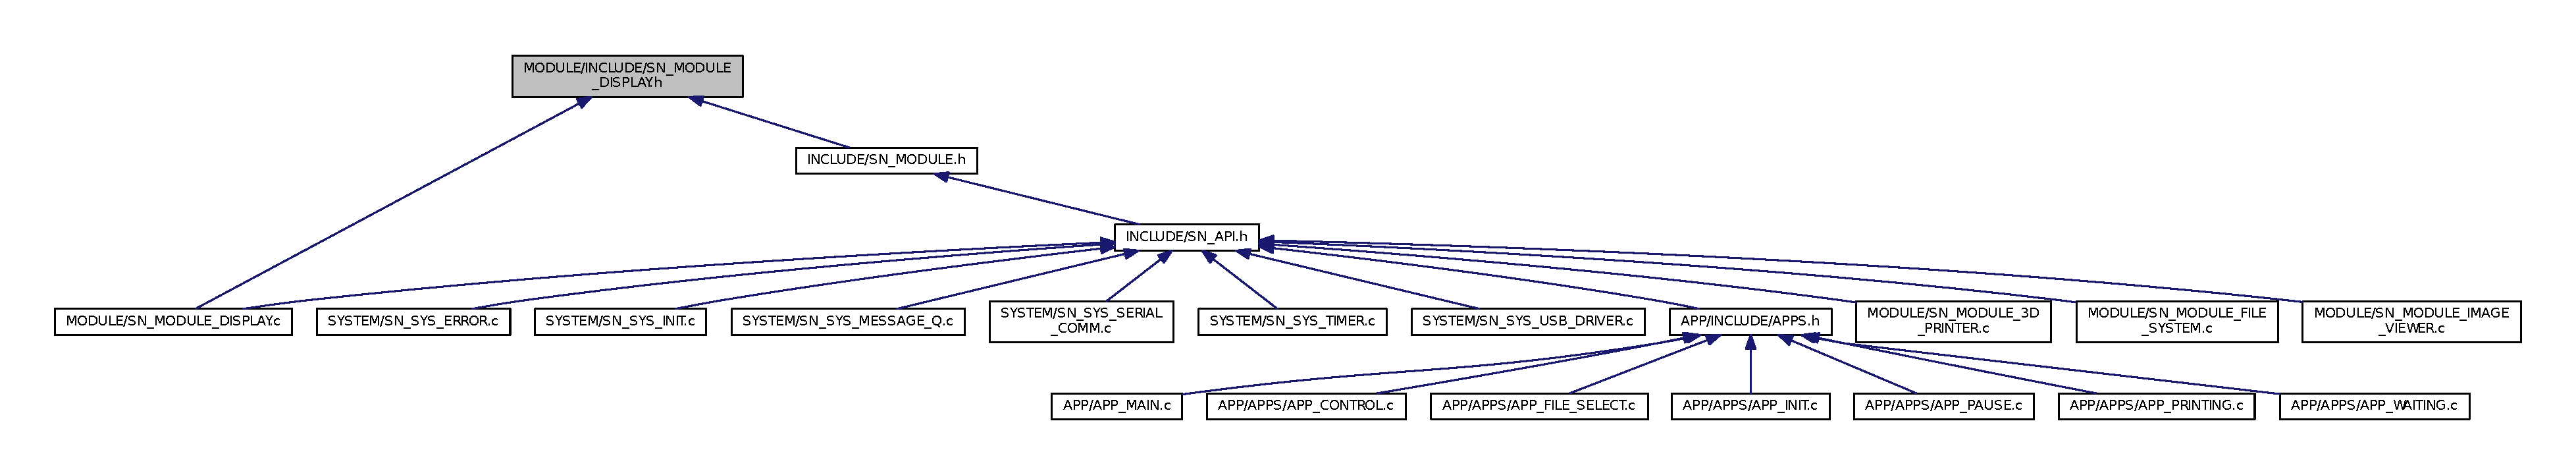
\includegraphics[width=350pt]{SN__MODULE__DISPLAY_8h__dep__incl}
\end{center}
\end{figure}
\subsection*{Functions}
\begin{Indent}\textbf{ Display Module}\par
{\em Description of Display Module Init and Uninit funtions. }\begin{DoxyCompactItemize}
\item 
\hyperlink{group__SYSTEM__ERROR_ga4540713b9a7a18ce44d78c3a10f7442f}{S\+N\+\_\+\+S\+T\+A\+T\+US} \hyperlink{group__MODULE__DISPLAY_ga894da8d8618a3c3b5bf2533a3a04622c}{S\+N\+\_\+\+M\+O\+D\+U\+L\+E\+\_\+\+D\+I\+S\+P\+L\+A\+Y\+\_\+\+Init} (void)
\item 
\hyperlink{group__SYSTEM__ERROR_ga4540713b9a7a18ce44d78c3a10f7442f}{S\+N\+\_\+\+S\+T\+A\+T\+US} \hyperlink{group__MODULE__DISPLAY_ga91f86811b5f4b83be3296c64ccd253ec}{S\+N\+\_\+\+M\+O\+D\+U\+L\+E\+\_\+\+D\+I\+S\+P\+L\+A\+Y\+\_\+\+Uninit} (void)
\end{DoxyCompactItemize}
\end{Indent}
\begin{Indent}\textbf{ Display Module \+:\+: Page Change}\par
\begin{DoxyCompactItemize}
\item 
\hyperlink{group__SYSTEM__ERROR_ga4540713b9a7a18ce44d78c3a10f7442f}{S\+N\+\_\+\+S\+T\+A\+T\+US} \hyperlink{group__MODULE__DISPLAY_ga91ef90fbda58e050514b22a2a564a82d}{S\+N\+\_\+\+M\+O\+D\+U\+L\+E\+\_\+\+D\+I\+S\+P\+L\+A\+Y\+\_\+\+Enter\+State} (\hyperlink{group__SYSTEM__SERIAL__NEXTION_ga5fafecdc824650a917eca294500efa57}{nx\+\_\+page\+\_\+t} state)
\item 
\hyperlink{group__SYSTEM__ERROR_ga4540713b9a7a18ce44d78c3a10f7442f}{S\+N\+\_\+\+S\+T\+A\+T\+US} \hyperlink{group__MODULE__DISPLAY_gabbde75c3e1a0fe4ffc14492a4e42931b}{S\+N\+\_\+\+M\+O\+D\+U\+L\+E\+\_\+\+D\+I\+S\+P\+L\+A\+Y\+\_\+\+File\+Select\+Update} (uint32\+\_\+t page)
\end{DoxyCompactItemize}
\end{Indent}
\begin{Indent}\textbf{ Display Module \+:\+: Print Page Info}\par
\begin{DoxyCompactItemize}
\item 
\hyperlink{group__SYSTEM__ERROR_ga4540713b9a7a18ce44d78c3a10f7442f}{S\+N\+\_\+\+S\+T\+A\+T\+US} \hyperlink{group__MODULE__DISPLAY_ga6059a98606c93e2bd4bd2ffb68486e4c}{S\+N\+\_\+\+M\+O\+D\+U\+L\+E\+\_\+\+D\+I\+S\+P\+L\+A\+Y\+\_\+\+Printing\+Info\+Init} (const char $\ast$file\+Name, const char $\ast$option\+Name)
\item 
\hyperlink{group__SYSTEM__ERROR_ga4540713b9a7a18ce44d78c3a10f7442f}{S\+N\+\_\+\+S\+T\+A\+T\+US} \hyperlink{group__MODULE__DISPLAY_ga943b965a7a2e59a6c9f035c74c2c8735}{S\+N\+\_\+\+M\+O\+D\+U\+L\+E\+\_\+\+D\+I\+S\+P\+L\+A\+Y\+\_\+\+Printing\+Info\+Update} (uint32\+\_\+t slice, uint32\+\_\+t target\+Slice)
\end{DoxyCompactItemize}
\end{Indent}
\begin{Indent}\textbf{ Display Module \+:\+: Print Page Time Info}\par
\begin{DoxyCompactItemize}
\item 
\hyperlink{group__SYSTEM__ERROR_ga4540713b9a7a18ce44d78c3a10f7442f}{S\+N\+\_\+\+S\+T\+A\+T\+US} \hyperlink{group__MODULE__DISPLAY_gac630c6bd386295f3008bc04e8b9c92a0}{S\+N\+\_\+\+M\+O\+D\+U\+L\+E\+\_\+\+D\+I\+S\+P\+L\+A\+Y\+\_\+\+Printing\+Timer\+Init} (uint32\+\_\+t sec)
\item 
\hyperlink{group__SYSTEM__ERROR_ga4540713b9a7a18ce44d78c3a10f7442f}{S\+N\+\_\+\+S\+T\+A\+T\+US} \hyperlink{group__MODULE__DISPLAY_ga21d62aed53ed746d4912685df22c224a}{S\+N\+\_\+\+M\+O\+D\+U\+L\+E\+\_\+\+D\+I\+S\+P\+L\+A\+Y\+\_\+\+Printing\+Timer\+Pause} (void)
\item 
\hyperlink{group__SYSTEM__ERROR_ga4540713b9a7a18ce44d78c3a10f7442f}{S\+N\+\_\+\+S\+T\+A\+T\+US} \hyperlink{group__MODULE__DISPLAY_ga457dd831602b689bb557899b06e69e3c}{S\+N\+\_\+\+M\+O\+D\+U\+L\+E\+\_\+\+D\+I\+S\+P\+L\+A\+Y\+\_\+\+Printing\+Timer\+Resume} (void)
\item 
\hyperlink{group__SYSTEM__ERROR_ga4540713b9a7a18ce44d78c3a10f7442f}{S\+N\+\_\+\+S\+T\+A\+T\+US} \hyperlink{group__MODULE__DISPLAY_ga23a40fbba57f5da86b6173fe40861196}{S\+N\+\_\+\+M\+O\+D\+U\+L\+E\+\_\+\+D\+I\+S\+P\+L\+A\+Y\+\_\+\+Printing\+Timer\+Stop} (void)
\end{DoxyCompactItemize}
\end{Indent}


\subsection{Detailed Description}
\begin{DoxyAuthor}{Author}
Bato 
\end{DoxyAuthor}
\begin{DoxyDate}{Date}
18 Sep 2018 
\end{DoxyDate}
\begin{DoxySeeAlso}{See also}
\href{http://www.stack.nl/~dimitri/doxygen/docblocks.html}{\tt http\+://www.\+stack.\+nl/$\sim$dimitri/doxygen/docblocks.\+html} 

\href{http://www.stack.nl/~dimitri/doxygen/commands.html}{\tt http\+://www.\+stack.\+nl/$\sim$dimitri/doxygen/commands.\+html} 
\end{DoxySeeAlso}

\hypertarget{SN__MODULE__FILE__SYSTEM_8h}{}\section{M\+O\+D\+U\+L\+E/\+I\+N\+C\+L\+U\+D\+E/\+S\+N\+\_\+\+M\+O\+D\+U\+L\+E\+\_\+\+F\+I\+L\+E\+\_\+\+S\+Y\+S\+T\+EM.h File Reference}
\label{SN__MODULE__FILE__SYSTEM_8h}\index{M\+O\+D\+U\+L\+E/\+I\+N\+C\+L\+U\+D\+E/\+S\+N\+\_\+\+M\+O\+D\+U\+L\+E\+\_\+\+F\+I\+L\+E\+\_\+\+S\+Y\+S\+T\+E\+M.\+h@{M\+O\+D\+U\+L\+E/\+I\+N\+C\+L\+U\+D\+E/\+S\+N\+\_\+\+M\+O\+D\+U\+L\+E\+\_\+\+F\+I\+L\+E\+\_\+\+S\+Y\+S\+T\+E\+M.\+h}}
This graph shows which files directly or indirectly include this file\+:\nopagebreak
\begin{figure}[H]
\begin{center}
\leavevmode
\includegraphics[width=350pt]{SN__MODULE__FILE__SYSTEM_8h__dep__incl}
\end{center}
\end{figure}
\subsection*{Classes}
\begin{DoxyCompactItemize}
\item 
struct \hyperlink{structfile__system__option}{file\+\_\+system\+\_\+option}
\item 
struct \hyperlink{structfile__system__item}{file\+\_\+system\+\_\+item}
\item 
struct \hyperlink{structfile__system__page}{file\+\_\+system\+\_\+page}
\item 
struct \hyperlink{structfile__system__target}{file\+\_\+system\+\_\+target}
\item 
struct \hyperlink{structfile__system}{file\+\_\+system}
\item 
struct \hyperlink{structprint__prameter}{print\+\_\+prameter}
\item 
struct \hyperlink{structprint__target}{print\+\_\+target}
\item 
struct \hyperlink{structprint__information}{print\+\_\+information}
\item 
struct \hyperlink{structmachine__information}{machine\+\_\+information}
\end{DoxyCompactItemize}
\subsection*{Macros}
\begin{Indent}\textbf{ File Sysetm Define}\par
\begin{DoxyCompactItemize}
\item 
\#define {\bfseries M\+A\+X\+\_\+\+P\+A\+G\+E\+\_\+\+S\+I\+ZE}~10
\item 
\#define {\bfseries M\+A\+X\+\_\+\+I\+T\+E\+M\+\_\+\+S\+I\+ZE}~5
\item 
\#define {\bfseries M\+A\+X\+\_\+\+O\+P\+T\+I\+O\+N\+\_\+\+S\+I\+ZE}~5
\item 
\#define {\bfseries M\+A\+X\+\_\+\+F\+I\+L\+E\+N\+A\+M\+E\+\_\+\+L\+E\+N\+G\+TH}~256
\item 
\#define {\bfseries M\+A\+X\+\_\+\+P\+A\+T\+H\+\_\+\+L\+E\+N\+G\+TH}~256
\end{DoxyCompactItemize}
\end{Indent}
\subsection*{Typedefs}
\begin{Indent}\textbf{ File System Structure}\par
\begin{DoxyCompactItemize}
\item 
typedef struct \hyperlink{structfile__system__option}{file\+\_\+system\+\_\+option} {\bfseries fs\+Option\+\_\+t}
\item 
typedef struct \hyperlink{structfile__system__item}{file\+\_\+system\+\_\+item} {\bfseries fs\+Item\+\_\+t}
\item 
typedef struct \hyperlink{structfile__system__page}{file\+\_\+system\+\_\+page} {\bfseries fs\+Page\+\_\+t}
\item 
typedef struct \hyperlink{structfile__system__target}{file\+\_\+system\+\_\+target} {\bfseries fs\+Target\+\_\+t}
\item 
typedef struct \hyperlink{structfile__system}{file\+\_\+system} {\bfseries fs\+\_\+t}
\end{DoxyCompactItemize}
\end{Indent}
\begin{Indent}\textbf{ Print Info Structure}\par
\begin{DoxyCompactItemize}
\item 
typedef struct \hyperlink{structprint__prameter}{print\+\_\+prameter} {\bfseries print\+Parm\+\_\+t}
\item 
typedef struct \hyperlink{structprint__target}{print\+\_\+target} {\bfseries print\+Target\+\_\+t}
\item 
typedef struct \hyperlink{structprint__information}{print\+\_\+information} {\bfseries print\+Info\+\_\+t}
\end{DoxyCompactItemize}
\end{Indent}
\begin{Indent}\textbf{ Machine Info Structure}\par
\begin{DoxyCompactItemize}
\item 
typedef struct \hyperlink{structmachine__information}{machine\+\_\+information} {\bfseries machine\+Info\+\_\+t}
\end{DoxyCompactItemize}
\end{Indent}
\subsection*{Functions}
\begin{DoxyCompactItemize}
\item 
\hyperlink{group__SYSTEM__ERROR_ga4540713b9a7a18ce44d78c3a10f7442f}{S\+N\+\_\+\+S\+T\+A\+T\+US} \hyperlink{group__MODULE__FILE__SYSTEM_ga4b8101916d7de3e4d3004b79f4c8c2de}{S\+N\+\_\+\+M\+O\+D\+U\+L\+E\+\_\+\+F\+I\+L\+E\+\_\+\+S\+Y\+S\+T\+E\+M\+\_\+\+Init} (void)
\item 
\hyperlink{group__SYSTEM__ERROR_ga4540713b9a7a18ce44d78c3a10f7442f}{S\+N\+\_\+\+S\+T\+A\+T\+US} \hyperlink{group__MODULE__FILE__SYSTEM_ga39c0e153f169cc6bdb35bce4d2a9194b}{S\+N\+\_\+\+M\+O\+D\+U\+L\+E\+\_\+\+F\+I\+L\+E\+\_\+\+S\+Y\+S\+T\+E\+M\+\_\+\+Uninit} (void)
\item 
\hyperlink{group__SYSTEM__ERROR_ga4540713b9a7a18ce44d78c3a10f7442f}{S\+N\+\_\+\+S\+T\+A\+T\+US} \hyperlink{group__MODULE__FILE__SYSTEM_gadfe4c4eeb9c662e30893824357bc46a5}{S\+N\+\_\+\+M\+O\+D\+U\+L\+E\+\_\+\+F\+I\+L\+E\+\_\+\+S\+Y\+S\+T\+E\+M\+\_\+\+Get} (\hyperlink{structfile__system}{fs\+\_\+t} $\ast$p\+Fs)
\item 
\hyperlink{group__SYSTEM__ERROR_ga4540713b9a7a18ce44d78c3a10f7442f}{S\+N\+\_\+\+S\+T\+A\+T\+US} \hyperlink{group__MODULE__FILE__SYSTEM_ga7df4490475224028341c54f5d5db5736}{S\+N\+\_\+\+M\+O\+D\+U\+L\+E\+\_\+\+F\+I\+L\+E\+\_\+\+S\+Y\+S\+T\+E\+M\+\_\+\+Update} (void)
\item 
\hyperlink{group__SYSTEM__ERROR_ga4540713b9a7a18ce44d78c3a10f7442f}{S\+N\+\_\+\+S\+T\+A\+T\+US} \hyperlink{group__MODULE__FILE__SYSTEM_ga4fba82e15bc9a77407cacaa1a6aadd50}{S\+N\+\_\+\+M\+O\+D\+U\+L\+E\+\_\+\+F\+I\+L\+E\+\_\+\+S\+Y\+S\+T\+E\+M\+\_\+\+Machine\+Info\+Init} (void)
\item 
\hyperlink{group__SYSTEM__ERROR_ga4540713b9a7a18ce44d78c3a10f7442f}{S\+N\+\_\+\+S\+T\+A\+T\+US} \hyperlink{group__MODULE__FILE__SYSTEM_ga86125af6adcd6218d4ebdb484e11d273}{S\+N\+\_\+\+M\+O\+D\+U\+L\+E\+\_\+\+F\+I\+L\+E\+\_\+\+S\+Y\+S\+T\+E\+M\+\_\+\+Machine\+Info\+Uninit} (void)
\item 
\hyperlink{structmachine__information}{machine\+Info\+\_\+t} \hyperlink{group__MODULE__FILE__SYSTEM_ga647e18cfc2415cb546d69b327ed76232}{S\+N\+\_\+\+M\+O\+D\+U\+L\+E\+\_\+\+F\+I\+L\+E\+\_\+\+S\+Y\+S\+T\+E\+M\+\_\+\+Machine\+Info\+Get} (void)
\item 
\hyperlink{group__SYSTEM__ERROR_ga4540713b9a7a18ce44d78c3a10f7442f}{S\+N\+\_\+\+S\+T\+A\+T\+US} \hyperlink{group__MODULE__FILE__SYSTEM_gadbd5aafed31faed399abd08193a04bc8}{S\+N\+\_\+\+M\+O\+D\+U\+L\+E\+\_\+\+F\+I\+L\+E\+\_\+\+S\+Y\+S\+T\+E\+M\+\_\+\+Print\+Info\+Init} (uint32\+\_\+t page\+Index, uint32\+\_\+t item\+Index)
\item 
\hyperlink{group__SYSTEM__ERROR_ga4540713b9a7a18ce44d78c3a10f7442f}{S\+N\+\_\+\+S\+T\+A\+T\+US} \hyperlink{group__MODULE__FILE__SYSTEM_gaddd6a0e37c98d7a5aba88db31875e44e}{S\+N\+\_\+\+M\+O\+D\+U\+L\+E\+\_\+\+F\+I\+L\+E\+\_\+\+S\+Y\+S\+T\+E\+M\+\_\+\+Print\+Info\+Uninit} (void)
\item 
\hyperlink{structprint__information}{print\+Info\+\_\+t} \hyperlink{group__MODULE__FILE__SYSTEM_ga6679d04769a997531a277ba3940cf16c}{S\+N\+\_\+\+M\+O\+D\+U\+L\+E\+\_\+\+F\+I\+L\+E\+\_\+\+S\+Y\+S\+T\+E\+M\+\_\+\+Print\+Info\+Get} (void)
\end{DoxyCompactItemize}


\subsection{Detailed Description}
\begin{DoxyAuthor}{Author}
Bato 
\end{DoxyAuthor}
\begin{DoxyDate}{Date}
1 Sep 2018 
\end{DoxyDate}
\begin{DoxySeeAlso}{See also}
\href{http://www.stack.nl/~dimitri/doxygen/docblocks.html}{\tt http\+://www.\+stack.\+nl/$\sim$dimitri/doxygen/docblocks.\+html} 

\href{http://www.stack.nl/~dimitri/doxygen/commands.html}{\tt http\+://www.\+stack.\+nl/$\sim$dimitri/doxygen/commands.\+html} 
\end{DoxySeeAlso}

\hypertarget{SN__MODULE__IMAGE__VIEWER_8h}{}\section{M\+O\+D\+U\+L\+E/\+I\+N\+C\+L\+U\+D\+E/\+S\+N\+\_\+\+M\+O\+D\+U\+L\+E\+\_\+\+I\+M\+A\+G\+E\+\_\+\+V\+I\+E\+W\+ER.h File Reference}
\label{SN__MODULE__IMAGE__VIEWER_8h}\index{M\+O\+D\+U\+L\+E/\+I\+N\+C\+L\+U\+D\+E/\+S\+N\+\_\+\+M\+O\+D\+U\+L\+E\+\_\+\+I\+M\+A\+G\+E\+\_\+\+V\+I\+E\+W\+E\+R.\+h@{M\+O\+D\+U\+L\+E/\+I\+N\+C\+L\+U\+D\+E/\+S\+N\+\_\+\+M\+O\+D\+U\+L\+E\+\_\+\+I\+M\+A\+G\+E\+\_\+\+V\+I\+E\+W\+E\+R.\+h}}
This graph shows which files directly or indirectly include this file\+:\nopagebreak
\begin{figure}[H]
\begin{center}
\leavevmode
\includegraphics[width=350pt]{SN__MODULE__IMAGE__VIEWER_8h__dep__incl}
\end{center}
\end{figure}
\subsection*{Functions}
\begin{Indent}\textbf{ Image Viewer Module}\par
{\em Description of Display Module Init and Uninit funtions. }\begin{DoxyCompactItemize}
\item 
\hyperlink{group__SYSTEM__ERROR_ga4540713b9a7a18ce44d78c3a10f7442f}{S\+N\+\_\+\+S\+T\+A\+T\+US} \hyperlink{group__MODULE__IMAGE__VIEWER_gafd26cb5c7532488dc8e0c37f07d16092}{S\+N\+\_\+\+M\+O\+D\+U\+L\+E\+\_\+\+I\+M\+A\+G\+E\+\_\+\+V\+I\+E\+W\+E\+R\+\_\+\+Init} (void)
\item 
\hyperlink{group__SYSTEM__ERROR_ga4540713b9a7a18ce44d78c3a10f7442f}{S\+N\+\_\+\+S\+T\+A\+T\+US} \hyperlink{group__MODULE__IMAGE__VIEWER_gae8357323213bf36b0a0011974f7c43dc}{S\+N\+\_\+\+M\+O\+D\+U\+L\+E\+\_\+\+I\+M\+A\+G\+E\+\_\+\+V\+I\+E\+W\+E\+R\+\_\+\+Destroy} (void)
\end{DoxyCompactItemize}
\end{Indent}
\begin{Indent}\textbf{ Image Viewer Module \+:\+: Printing}\par
\begin{DoxyCompactItemize}
\item 
\hyperlink{group__SYSTEM__ERROR_ga4540713b9a7a18ce44d78c3a10f7442f}{S\+N\+\_\+\+S\+T\+A\+T\+US} \hyperlink{group__MODULE__IMAGE__VIEWER_ga16b58f3bf4681b8ccda18d88490456a7}{S\+N\+\_\+\+M\+O\+D\+U\+L\+E\+\_\+\+I\+M\+A\+G\+E\+\_\+\+V\+I\+E\+W\+E\+R\+\_\+\+U\+P\+D\+A\+TE} (uint32\+\_\+t slice\+Index)
\end{DoxyCompactItemize}
\end{Indent}
\begin{Indent}\textbf{ Image Viewer Module \+:\+: Screen Control}\par
\begin{DoxyCompactItemize}
\item 
\hyperlink{group__SYSTEM__ERROR_ga4540713b9a7a18ce44d78c3a10f7442f}{S\+N\+\_\+\+S\+T\+A\+T\+US} \hyperlink{group__MODULE__IMAGE__VIEWER_ga77d2b7a49b61f4edf67ffc2466a032dd}{S\+N\+\_\+\+M\+O\+D\+U\+L\+E\+\_\+\+I\+M\+A\+G\+E\+\_\+\+V\+I\+E\+W\+E\+R\+\_\+\+C\+L\+E\+AR} (void)
\end{DoxyCompactItemize}
\end{Indent}


\subsection{Detailed Description}
\begin{DoxyAuthor}{Author}
Bato 
\end{DoxyAuthor}
\begin{DoxyDate}{Date}
1 Sep 2018 
\end{DoxyDate}
\begin{DoxySeeAlso}{See also}
\href{http://www.stack.nl/~dimitri/doxygen/docblocks.html}{\tt http\+://www.\+stack.\+nl/$\sim$dimitri/doxygen/docblocks.\+html} 

\href{http://www.stack.nl/~dimitri/doxygen/commands.html}{\tt http\+://www.\+stack.\+nl/$\sim$dimitri/doxygen/commands.\+html} 
\end{DoxySeeAlso}

\hypertarget{SN__MODULE__3D__PRINTER_8c}{}\section{M\+O\+D\+U\+L\+E/\+S\+N\+\_\+\+M\+O\+D\+U\+L\+E\+\_\+3\+D\+\_\+\+P\+R\+I\+N\+T\+ER.c File Reference}
\label{SN__MODULE__3D__PRINTER_8c}\index{M\+O\+D\+U\+L\+E/\+S\+N\+\_\+\+M\+O\+D\+U\+L\+E\+\_\+3\+D\+\_\+\+P\+R\+I\+N\+T\+E\+R.\+c@{M\+O\+D\+U\+L\+E/\+S\+N\+\_\+\+M\+O\+D\+U\+L\+E\+\_\+3\+D\+\_\+\+P\+R\+I\+N\+T\+E\+R.\+c}}
{\ttfamily \#include \char`\"{}S\+N\+\_\+\+A\+P\+I.\+h\char`\"{}}\newline
{\ttfamily \#include \char`\"{}S\+N\+\_\+\+M\+O\+D\+U\+L\+E\+\_\+3\+D\+\_\+\+P\+R\+I\+N\+T\+E\+R.\+h\char`\"{}}\newline
{\ttfamily \#include \char`\"{}S\+N\+\_\+\+M\+O\+D\+U\+L\+E\+\_\+\+I\+M\+A\+G\+E\+\_\+\+V\+I\+E\+W\+E\+R.\+h\char`\"{}}\newline
Include dependency graph for S\+N\+\_\+\+M\+O\+D\+U\+L\+E\+\_\+3\+D\+\_\+\+P\+R\+I\+N\+T\+E\+R.\+c\+:\nopagebreak
\begin{figure}[H]
\begin{center}
\leavevmode
\includegraphics[width=350pt]{SN__MODULE__3D__PRINTER_8c__incl}
\end{center}
\end{figure}
\subsection*{Classes}
\begin{DoxyCompactItemize}
\item 
struct \hyperlink{structmoduel__3d__printer}{moduel\+\_\+3d\+\_\+printer}
\end{DoxyCompactItemize}
\subsection*{Macros}
\begin{DoxyCompactItemize}
\item 
\#define \hyperlink{SN__MODULE__3D__PRINTER_8c_a361e946e2049940ce6a56caddf5a18f0}{E\+S\+T\+I\+M\+A\+T\+E\+D\+\_\+\+B\+U\+I\+L\+D\+\_\+\+T\+I\+M\+E\+\_\+\+S\+E\+C\+\_\+\+C\+AL}(z\+\_\+delay,  uv\+\_\+delay,  uv\+\_\+bottom\+\_\+deleay,  num\+\_\+of\+\_\+layer,  num\+\_\+of\+\_\+bottom\+\_\+layer)~((((z\+\_\+delay) + (uv\+\_\+delay)) / 1000) $\ast$ ((num\+\_\+of\+\_\+layer) -\/ (num\+\_\+of\+\_\+bottom\+\_\+layer)) + (((uv\+\_\+bottom\+\_\+deleay + z\+\_\+delay) / 1000) $\ast$ (num\+\_\+of\+\_\+bottom\+\_\+layer)))
\begin{DoxyCompactList}\small\item\em estimated build time calculator E\+S\+T\+I\+M\+A\+T\+E\+D\+\_\+\+B\+U\+I\+L\+D\+\_\+\+T\+I\+M\+E\+\_\+\+S\+E\+C\+\_\+\+C\+AL -\/ Def. funtion \end{DoxyCompactList}\end{DoxyCompactItemize}
\begin{Indent}\textbf{ Serial Config Define}\par
\begin{DoxyCompactItemize}
\item 
\mbox{\Hypertarget{SN__MODULE__3D__PRINTER_8c_a86fd4404b140711fdb77326609c0f393}\label{SN__MODULE__3D__PRINTER_8c_a86fd4404b140711fdb77326609c0f393}} 
\#define {\bfseries B\+Y\+T\+E\+\_\+\+S\+I\+ZE}~\hyperlink{group__SYSTEM__SERIAL__COMM_ga45345dabcfb671abba160a3dac350670}{S\+N\+\_\+\+S\+Y\+S\+\_\+\+S\+E\+R\+I\+A\+L\+\_\+\+C\+O\+M\+M\+\_\+\+R\+X\+\_\+\+R\+E\+A\+L\+T\+I\+ME}
\item 
\mbox{\Hypertarget{SN__MODULE__3D__PRINTER_8c_ad4455691936f92fdd6c37566fc58ba1f}\label{SN__MODULE__3D__PRINTER_8c_ad4455691936f92fdd6c37566fc58ba1f}} 
\#define {\bfseries B\+A\+U\+D\+\_\+\+R\+A\+TE}~\hyperlink{group__SYSTEM__SERIAL__COMM_gac225ef6708a36c14757361c4f496f218}{S\+N\+\_\+\+S\+Y\+S\+\_\+\+S\+E\+R\+I\+A\+L\+\_\+\+C\+O\+M\+M\+\_\+\+B\+A\+U\+D\+\_\+\+R\+A\+T\+E\+\_\+115200}
\item 
\mbox{\Hypertarget{SN__MODULE__3D__PRINTER_8c_a5a0f6d20bbd813bb42026be07a61546b}\label{SN__MODULE__3D__PRINTER_8c_a5a0f6d20bbd813bb42026be07a61546b}} 
\#define {\bfseries R\+E\+T\+U\+R\+N\+\_\+\+M\+O\+DE}~\hyperlink{group__SYSTEM__SERIAL__COMM_ga96c2a829d5aa963c53ee3f5607ef22fa}{S\+N\+\_\+\+S\+Y\+S\+\_\+\+S\+E\+R\+I\+A\+L\+\_\+\+C\+O\+M\+M\+\_\+\+T\+X\+\_\+\+N\+E\+W\+\_\+\+L\+I\+N\+E\+\_\+\+R\+E\+T\+U\+RN}
\item 
\mbox{\Hypertarget{SN__MODULE__3D__PRINTER_8c_ade98bd4cd04d126a2dec0f4e0ab55650}\label{SN__MODULE__3D__PRINTER_8c_ade98bd4cd04d126a2dec0f4e0ab55650}} 
\#define {\bfseries U\+A\+R\+T\+\_\+\+O\+F\+L\+A\+GS}~(O\+\_\+\+R\+D\+WR $\vert$ O\+\_\+\+N\+O\+C\+T\+TY $\vert$ O\+\_\+\+N\+O\+N\+B\+L\+O\+CK)
\end{DoxyCompactItemize}
\end{Indent}
\begin{Indent}\textbf{ Printing Config Define}\par
\begin{DoxyCompactItemize}
\item 
\#define \hyperlink{SN__MODULE__3D__PRINTER_8c_a8d035fd9f86fac533b2d33534c0bcef4}{F\+I\+R\+S\+T\+\_\+\+S\+L\+I\+C\+E\+\_\+\+D\+E\+L\+A\+Y\+\_\+\+T\+I\+ME}~5000
\item 
\#define \hyperlink{SN__MODULE__3D__PRINTER_8c_afe24acc5c3c3e5e44eddf6bcbc688f61}{F\+I\+N\+I\+S\+H\+\_\+\+D\+E\+V\+I\+C\+E\+\_\+\+D\+E\+L\+A\+Y\+\_\+\+T\+I\+ME}~50000
\item 
\#define \hyperlink{SN__MODULE__3D__PRINTER_8c_aa566db1a40d3471fc620d23519912482}{S\+T\+O\+P\+\_\+\+D\+E\+V\+I\+C\+E\+\_\+\+D\+E\+L\+A\+Y\+\_\+\+T\+I\+ME}~10000
\end{DoxyCompactItemize}
\end{Indent}
\begin{Indent}\textbf{ Other Define}\par
\begin{DoxyCompactItemize}
\item 
\#define \hyperlink{SN__MODULE__3D__PRINTER_8c_af6168edd26520974b8660182d040051a}{G\+C\+O\+D\+E\+\_\+\+B\+U\+F\+F\+E\+R\+\_\+\+S\+I\+ZE}~30
\item 
\#define \hyperlink{SN__MODULE__3D__PRINTER_8c_ad77a467852ad83019914973d6e2c6d31}{I\+N\+P\+U\+T\+\_\+\+C\+H\+A\+I\+N\+\_\+\+C\+O\+N\+D\+I\+T\+I\+ON}~3
\end{DoxyCompactItemize}
\end{Indent}
\subsection*{Typedefs}
\begin{DoxyCompactItemize}
\item 
\mbox{\Hypertarget{SN__MODULE__3D__PRINTER_8c_abf9b3bbf15e03173bb845afefee07c90}\label{SN__MODULE__3D__PRINTER_8c_abf9b3bbf15e03173bb845afefee07c90}} 
typedef enum \hyperlink{SN__MODULE__3D__PRINTER_8c_a3322f575207e76f4d154936e39196d0f}{device\+\_\+state} {\bfseries device\+State\+\_\+t}
\item 
\mbox{\Hypertarget{SN__MODULE__3D__PRINTER_8c_af33dc15f9be15faf2dc925f41819b798}\label{SN__MODULE__3D__PRINTER_8c_af33dc15f9be15faf2dc925f41819b798}} 
typedef struct \hyperlink{structmoduel__3d__printer}{moduel\+\_\+3d\+\_\+printer} {\bfseries module3\+D\+Printer\+\_\+t}
\item 
\mbox{\Hypertarget{SN__MODULE__3D__PRINTER_8c_ad278b5768d77c0eca20256550b4a478f}\label{SN__MODULE__3D__PRINTER_8c_ad278b5768d77c0eca20256550b4a478f}} 
typedef enum \hyperlink{SN__MODULE__3D__PRINTER_8c_ace39a9a0abfec103d37b5f252401e93c}{event\+\_\+3d\+\_\+printer\+\_\+message} {\bfseries evt3\+D\+Printer\+\_\+t}
\end{DoxyCompactItemize}
\subsection*{Enumerations}
\begin{DoxyCompactItemize}
\item 
enum \hyperlink{SN__MODULE__3D__PRINTER_8c_a3322f575207e76f4d154936e39196d0f}{device\+\_\+state} \{ \newline
\hyperlink{SN__MODULE__3D__PRINTER_8c_a3322f575207e76f4d154936e39196d0fac4141ec776a3f91250778842cb3cca7d}{D\+E\+V\+I\+C\+E\+\_\+\+S\+T\+A\+N\+D\+BY}, 
\hyperlink{SN__MODULE__3D__PRINTER_8c_a3322f575207e76f4d154936e39196d0fa5b3e76c02f24f0d0df34a05a0da59358}{D\+E\+V\+I\+C\+E\+\_\+\+I\+N\+IT}, 
\hyperlink{SN__MODULE__3D__PRINTER_8c_a3322f575207e76f4d154936e39196d0fa14ba6379ebff00cfbb75cc348d22954c}{D\+E\+V\+I\+C\+E\+\_\+\+P\+R\+I\+N\+T\+I\+NG}, 
\hyperlink{SN__MODULE__3D__PRINTER_8c_a3322f575207e76f4d154936e39196d0fa80a47159ec3a8bea095ff5f2463ad98d}{D\+E\+V\+I\+C\+E\+\_\+\+P\+A\+U\+SE}, 
\newline
\hyperlink{SN__MODULE__3D__PRINTER_8c_a3322f575207e76f4d154936e39196d0faa6c5e5acbc9c3626c1ef2c894015d6d1}{D\+E\+V\+I\+C\+E\+\_\+\+R\+E\+S\+U\+ME}, 
\hyperlink{SN__MODULE__3D__PRINTER_8c_a3322f575207e76f4d154936e39196d0fa5739343ed25c72f71fa6f9456c3ea945}{D\+E\+V\+I\+C\+E\+\_\+\+S\+T\+OP}, 
\hyperlink{SN__MODULE__3D__PRINTER_8c_a3322f575207e76f4d154936e39196d0fad2582b0500a849ebbc11916b84211e36}{D\+E\+V\+I\+C\+E\+\_\+\+F\+I\+N\+I\+SH}, 
\hyperlink{SN__MODULE__3D__PRINTER_8c_a3322f575207e76f4d154936e39196d0fab2185057f66cb8d6b7ea99f146be11f2}{D\+E\+V\+I\+C\+E\+\_\+\+B\+U\+SY}, 
\newline
\hyperlink{SN__MODULE__3D__PRINTER_8c_a3322f575207e76f4d154936e39196d0fa3e302cce6b1fef39d1af5c09dcc5cd1f}{D\+E\+V\+I\+C\+E\+\_\+\+H\+O\+M\+I\+NG}, 
\hyperlink{SN__MODULE__3D__PRINTER_8c_a3322f575207e76f4d154936e39196d0fa50c30a23dea6c506c49b17b601ae2c4e}{D\+E\+V\+I\+C\+E\+\_\+\+N\+O\+NE}
 \}
\item 
enum \hyperlink{SN__MODULE__3D__PRINTER_8c_ace39a9a0abfec103d37b5f252401e93c}{event\+\_\+3d\+\_\+printer\+\_\+message} \{ \newline
\hyperlink{SN__MODULE__3D__PRINTER_8c_ace39a9a0abfec103d37b5f252401e93caeb12ed6755f90036a6def274f1705834}{M\+S\+G\+\_\+3\+D\+\_\+\+P\+R\+I\+N\+T\+E\+R\+\_\+\+P\+R\+I\+N\+T\+I\+N\+G\+\_\+\+I\+N\+IT} = 0, 
\hyperlink{SN__MODULE__3D__PRINTER_8c_ace39a9a0abfec103d37b5f252401e93ca29c3bab34c0834e23b9a6f0567d88776}{M\+S\+G\+\_\+3\+D\+\_\+\+P\+R\+I\+N\+T\+E\+R\+\_\+\+P\+R\+I\+N\+T\+I\+N\+G\+\_\+\+C\+Y\+C\+LE}, 
\hyperlink{SN__MODULE__3D__PRINTER_8c_ace39a9a0abfec103d37b5f252401e93ca239c3c1de600da086e8af2750b8666c2}{M\+S\+G\+\_\+3\+D\+\_\+\+P\+R\+I\+N\+T\+E\+R\+\_\+\+P\+R\+I\+N\+T\+I\+N\+G\+\_\+\+Z\+\_\+\+L\+I\+FT}, 
\hyperlink{SN__MODULE__3D__PRINTER_8c_ace39a9a0abfec103d37b5f252401e93caf613e9f9d380fd82e6c5861570afe65f}{M\+S\+G\+\_\+3\+D\+\_\+\+P\+R\+I\+N\+T\+E\+R\+\_\+\+P\+R\+I\+N\+T\+I\+N\+G\+\_\+\+P\+A\+U\+SE}, 
\newline
\hyperlink{SN__MODULE__3D__PRINTER_8c_ace39a9a0abfec103d37b5f252401e93caa25410b4a2f3a4d7dfeca849b95f54b1}{M\+S\+G\+\_\+3\+D\+\_\+\+P\+R\+I\+N\+T\+E\+R\+\_\+\+P\+R\+I\+N\+T\+I\+N\+G\+\_\+\+R\+E\+S\+U\+ME}, 
\hyperlink{SN__MODULE__3D__PRINTER_8c_ace39a9a0abfec103d37b5f252401e93cacfd3a8295b72d77dbd6fabe554793f2e}{M\+S\+G\+\_\+3\+D\+\_\+\+P\+R\+I\+N\+T\+E\+R\+\_\+\+P\+R\+I\+N\+T\+I\+N\+G\+\_\+\+S\+T\+OP}, 
\hyperlink{SN__MODULE__3D__PRINTER_8c_ace39a9a0abfec103d37b5f252401e93caf96c559fb8aa50e8c3d1b1713d44d4f2}{M\+S\+G\+\_\+3\+D\+\_\+\+P\+R\+I\+N\+T\+E\+R\+\_\+\+P\+R\+I\+N\+T\+I\+N\+G\+\_\+\+F\+I\+N\+I\+SH}, 
\hyperlink{SN__MODULE__3D__PRINTER_8c_ace39a9a0abfec103d37b5f252401e93ca095ce6291f7f4cf157e483c098990a98}{M\+S\+G\+\_\+3\+D\+\_\+\+P\+R\+I\+N\+T\+E\+R\+\_\+\+H\+O\+M\+M\+I\+NG}, 
\newline
\hyperlink{SN__MODULE__3D__PRINTER_8c_ace39a9a0abfec103d37b5f252401e93caeee5d7bc3016df70276e2d335cf371d3}{M\+S\+G\+\_\+3\+D\+\_\+\+P\+R\+I\+N\+T\+E\+R\+\_\+\+S\+T\+A\+N\+D\+BY}, 
\hyperlink{SN__MODULE__3D__PRINTER_8c_ace39a9a0abfec103d37b5f252401e93ca65e23858f476fe3a3937fe25c85ebb54}{M\+S\+G\+\_\+3\+D\+\_\+\+P\+R\+I\+N\+T\+E\+R\+\_\+\+N\+O\+NE}, 
\hyperlink{SN__MODULE__3D__PRINTER_8c_ace39a9a0abfec103d37b5f252401e93ca24940221cf155a9a11e79c4db630bb3c}{M\+S\+G\+\_\+3\+D\+\_\+\+P\+R\+I\+N\+T\+E\+R\+\_\+\+I\+G\+N\+O\+RE} = 0x\+F\+F01
 \}
\end{DoxyCompactItemize}
\subsection*{Functions}
\begin{DoxyCompactItemize}
\item 
\mbox{\Hypertarget{SN__MODULE__3D__PRINTER_8c_aadce2bdf1f6c733052e82bfcfe1ba944}\label{SN__MODULE__3D__PRINTER_8c_aadce2bdf1f6c733052e82bfcfe1ba944}} 
{\bfseries sys\+Serial\+Def} (3\+D\+Printer\+Serial, U\+A\+R\+T\+\_\+\+D\+E\+V\+I\+C\+E, U\+A\+R\+T\+\_\+\+O\+F\+L\+A\+G\+S, B\+A\+U\+D\+\_\+\+R\+A\+T\+E, B\+Y\+T\+E\+\_\+\+S\+I\+Z\+E, R\+E\+T\+U\+R\+N\+\_\+\+M\+O\+D\+E)
\item 
\hyperlink{group__SYSTEM__ERROR_ga4540713b9a7a18ce44d78c3a10f7442f}{S\+N\+\_\+\+S\+T\+A\+T\+US} {\bfseries S\+N\+\_\+\+M\+O\+D\+U\+L\+E\+\_\+3\+D\+\_\+\+P\+R\+I\+N\+T\+E\+R\+\_\+\+Test} (void)
\item 
\hyperlink{group__SYSTEM__ERROR_ga4540713b9a7a18ce44d78c3a10f7442f}{S\+N\+\_\+\+S\+T\+A\+T\+US} \hyperlink{group__MODULE__3D__PRINTER_ga801e265ffe6f8c56081112f4fdd35f39}{S\+N\+\_\+\+M\+O\+D\+U\+L\+E\+\_\+3\+D\+\_\+\+P\+R\+I\+N\+T\+E\+R\+\_\+\+Init} (void)
\item 
\hyperlink{group__SYSTEM__ERROR_ga4540713b9a7a18ce44d78c3a10f7442f}{S\+N\+\_\+\+S\+T\+A\+T\+US} \hyperlink{group__MODULE__3D__PRINTER_ga776f5e31b0c0e176e35669f9432baec0}{S\+N\+\_\+\+M\+O\+D\+U\+L\+E\+\_\+3\+D\+\_\+\+P\+R\+I\+N\+T\+E\+R\+\_\+\+Uninit} (void)
\item 
\hyperlink{group__SYSTEM__ERROR_ga4540713b9a7a18ce44d78c3a10f7442f}{S\+N\+\_\+\+S\+T\+A\+T\+US} \hyperlink{group__MODULE__3D__PRINTER_ga83ec7a117b45a5760e1aecde26f69dea}{S\+N\+\_\+\+M\+O\+D\+U\+L\+E\+\_\+3\+D\+\_\+\+P\+R\+I\+N\+T\+E\+R\+\_\+\+Motor\+Init} (void)
\item 
\hyperlink{group__SYSTEM__ERROR_ga4540713b9a7a18ce44d78c3a10f7442f}{S\+N\+\_\+\+S\+T\+A\+T\+US} \hyperlink{group__MODULE__3D__PRINTER_ga2f644e451b310348d50fef6c762bbbcc}{S\+N\+\_\+\+M\+O\+D\+U\+L\+E\+\_\+3\+D\+\_\+\+P\+R\+I\+N\+T\+E\+R\+\_\+\+Motor\+Uninit} (void)
\item 
\hyperlink{group__SYSTEM__ERROR_ga4540713b9a7a18ce44d78c3a10f7442f}{S\+N\+\_\+\+S\+T\+A\+T\+US} \hyperlink{group__MODULE__3D__PRINTER_ga7bba4aa3966da87ac001b67b301310c1}{S\+N\+\_\+\+M\+O\+D\+U\+L\+E\+\_\+3\+D\+\_\+\+P\+R\+I\+N\+T\+E\+R\+\_\+\+Z\+\_\+\+Homing} (void)
\item 
\hyperlink{group__SYSTEM__ERROR_ga4540713b9a7a18ce44d78c3a10f7442f}{S\+N\+\_\+\+S\+T\+A\+T\+US} \hyperlink{group__MODULE__3D__PRINTER_ga47326e9f9d52dae584ee7c12011efc64}{S\+N\+\_\+\+M\+O\+D\+U\+L\+E\+\_\+3\+D\+\_\+\+P\+R\+I\+N\+T\+E\+R\+\_\+\+Z\+\_\+\+Up} (float mm)
\item 
\hyperlink{group__SYSTEM__ERROR_ga4540713b9a7a18ce44d78c3a10f7442f}{S\+N\+\_\+\+S\+T\+A\+T\+US} \hyperlink{group__MODULE__3D__PRINTER_ga65e82d5d94b534427c5d036080e77cf0}{S\+N\+\_\+\+M\+O\+D\+U\+L\+E\+\_\+3\+D\+\_\+\+P\+R\+I\+N\+T\+E\+R\+\_\+\+Z\+\_\+\+Down} (float mm)
\item 
\hyperlink{group__SYSTEM__ERROR_ga4540713b9a7a18ce44d78c3a10f7442f}{S\+N\+\_\+\+S\+T\+A\+T\+US} \hyperlink{group__MODULE__3D__PRINTER_ga439ebb10f8ee839218655c5177e9110b}{S\+N\+\_\+\+M\+O\+D\+U\+L\+E\+\_\+3\+D\+\_\+\+P\+R\+I\+N\+T\+E\+R\+\_\+\+Start} (uint32\+\_\+t page\+Index, uint32\+\_\+t item\+Index)
\item 
\hyperlink{group__SYSTEM__ERROR_ga4540713b9a7a18ce44d78c3a10f7442f}{S\+N\+\_\+\+S\+T\+A\+T\+US} \hyperlink{group__MODULE__3D__PRINTER_ga84a03238ddc0021011c12839757bf8c2}{S\+N\+\_\+\+M\+O\+D\+U\+L\+E\+\_\+3\+D\+\_\+\+P\+R\+I\+N\+T\+E\+R\+\_\+\+Pause} (void)
\item 
\hyperlink{group__SYSTEM__ERROR_ga4540713b9a7a18ce44d78c3a10f7442f}{S\+N\+\_\+\+S\+T\+A\+T\+US} \hyperlink{group__MODULE__3D__PRINTER_gaabec8b5f01119d989d725eff26053ca5}{S\+N\+\_\+\+M\+O\+D\+U\+L\+E\+\_\+3\+D\+\_\+\+P\+R\+I\+N\+T\+E\+R\+\_\+\+Resume} (void)
\item 
\hyperlink{group__SYSTEM__ERROR_ga4540713b9a7a18ce44d78c3a10f7442f}{S\+N\+\_\+\+S\+T\+A\+T\+US} \hyperlink{group__MODULE__3D__PRINTER_ga21ca69a451fafe2c9218c9a1737e1f15}{S\+N\+\_\+\+M\+O\+D\+U\+L\+E\+\_\+3\+D\+\_\+\+P\+R\+I\+N\+T\+E\+R\+\_\+\+Stop} (void)
\end{DoxyCompactItemize}
\begin{Indent}\textbf{ Static Print Control Funtions}\par
{\em Description of Display Module Init and Uninit funtions. }\end{Indent}


\subsection{Detailed Description}
\begin{DoxyAuthor}{Author}
Bato 
\end{DoxyAuthor}
\begin{DoxyDate}{Date}
10 Oct 2018
\end{DoxyDate}
\begin{DoxySeeAlso}{See also}
\href{http://www.stack.nl/~dimitri/doxygen/docblocks.html}{\tt http\+://www.\+stack.\+nl/$\sim$dimitri/doxygen/docblocks.\+html} 

\href{http://www.stack.nl/~dimitri/doxygen/commands.html}{\tt http\+://www.\+stack.\+nl/$\sim$dimitri/doxygen/commands.\+html} 
\end{DoxySeeAlso}


\subsection{Macro Definition Documentation}
\mbox{\Hypertarget{SN__MODULE__3D__PRINTER_8c_a361e946e2049940ce6a56caddf5a18f0}\label{SN__MODULE__3D__PRINTER_8c_a361e946e2049940ce6a56caddf5a18f0}} 
\index{S\+N\+\_\+\+M\+O\+D\+U\+L\+E\+\_\+3\+D\+\_\+\+P\+R\+I\+N\+T\+E\+R.\+c@{S\+N\+\_\+\+M\+O\+D\+U\+L\+E\+\_\+3\+D\+\_\+\+P\+R\+I\+N\+T\+E\+R.\+c}!E\+S\+T\+I\+M\+A\+T\+E\+D\+\_\+\+B\+U\+I\+L\+D\+\_\+\+T\+I\+M\+E\+\_\+\+S\+E\+C\+\_\+\+C\+AL@{E\+S\+T\+I\+M\+A\+T\+E\+D\+\_\+\+B\+U\+I\+L\+D\+\_\+\+T\+I\+M\+E\+\_\+\+S\+E\+C\+\_\+\+C\+AL}}
\index{E\+S\+T\+I\+M\+A\+T\+E\+D\+\_\+\+B\+U\+I\+L\+D\+\_\+\+T\+I\+M\+E\+\_\+\+S\+E\+C\+\_\+\+C\+AL@{E\+S\+T\+I\+M\+A\+T\+E\+D\+\_\+\+B\+U\+I\+L\+D\+\_\+\+T\+I\+M\+E\+\_\+\+S\+E\+C\+\_\+\+C\+AL}!S\+N\+\_\+\+M\+O\+D\+U\+L\+E\+\_\+3\+D\+\_\+\+P\+R\+I\+N\+T\+E\+R.\+c@{S\+N\+\_\+\+M\+O\+D\+U\+L\+E\+\_\+3\+D\+\_\+\+P\+R\+I\+N\+T\+E\+R.\+c}}
\subsubsection{\texorpdfstring{E\+S\+T\+I\+M\+A\+T\+E\+D\+\_\+\+B\+U\+I\+L\+D\+\_\+\+T\+I\+M\+E\+\_\+\+S\+E\+C\+\_\+\+C\+AL}{ESTIMATED\_BUILD\_TIME\_SEC\_CAL}}
{\footnotesize\ttfamily \#define E\+S\+T\+I\+M\+A\+T\+E\+D\+\_\+\+B\+U\+I\+L\+D\+\_\+\+T\+I\+M\+E\+\_\+\+S\+E\+C\+\_\+\+C\+AL(\begin{DoxyParamCaption}\item[{}]{z\+\_\+delay,  }\item[{}]{uv\+\_\+delay,  }\item[{}]{uv\+\_\+bottom\+\_\+deleay,  }\item[{}]{num\+\_\+of\+\_\+layer,  }\item[{}]{num\+\_\+of\+\_\+bottom\+\_\+layer }\end{DoxyParamCaption})~((((z\+\_\+delay) + (uv\+\_\+delay)) / 1000) $\ast$ ((num\+\_\+of\+\_\+layer) -\/ (num\+\_\+of\+\_\+bottom\+\_\+layer)) + (((uv\+\_\+bottom\+\_\+deleay + z\+\_\+delay) / 1000) $\ast$ (num\+\_\+of\+\_\+bottom\+\_\+layer)))}



estimated build time calculator E\+S\+T\+I\+M\+A\+T\+E\+D\+\_\+\+B\+U\+I\+L\+D\+\_\+\+T\+I\+M\+E\+\_\+\+S\+E\+C\+\_\+\+C\+AL -\/ Def. funtion 


\begin{DoxyParams}{Parameters}
{\em z\+\_\+delay} & \\
\hline
{\em uv\+\_\+delay} & \\
\hline
{\em uv\+\_\+bottom\+\_\+delay} & \\
\hline
{\em num\+\_\+of\+\_\+layer} & \\
\hline
{\em num\+\_\+of\+\_\+bottom\+\_\+layer} & \\
\hline
\end{DoxyParams}
\begin{DoxyReturn}{Returns}
estimated build time (sec) 
\end{DoxyReturn}
\begin{DoxyNote}{Note}

\end{DoxyNote}
\mbox{\Hypertarget{SN__MODULE__3D__PRINTER_8c_afe24acc5c3c3e5e44eddf6bcbc688f61}\label{SN__MODULE__3D__PRINTER_8c_afe24acc5c3c3e5e44eddf6bcbc688f61}} 
\index{S\+N\+\_\+\+M\+O\+D\+U\+L\+E\+\_\+3\+D\+\_\+\+P\+R\+I\+N\+T\+E\+R.\+c@{S\+N\+\_\+\+M\+O\+D\+U\+L\+E\+\_\+3\+D\+\_\+\+P\+R\+I\+N\+T\+E\+R.\+c}!F\+I\+N\+I\+S\+H\+\_\+\+D\+E\+V\+I\+C\+E\+\_\+\+D\+E\+L\+A\+Y\+\_\+\+T\+I\+ME@{F\+I\+N\+I\+S\+H\+\_\+\+D\+E\+V\+I\+C\+E\+\_\+\+D\+E\+L\+A\+Y\+\_\+\+T\+I\+ME}}
\index{F\+I\+N\+I\+S\+H\+\_\+\+D\+E\+V\+I\+C\+E\+\_\+\+D\+E\+L\+A\+Y\+\_\+\+T\+I\+ME@{F\+I\+N\+I\+S\+H\+\_\+\+D\+E\+V\+I\+C\+E\+\_\+\+D\+E\+L\+A\+Y\+\_\+\+T\+I\+ME}!S\+N\+\_\+\+M\+O\+D\+U\+L\+E\+\_\+3\+D\+\_\+\+P\+R\+I\+N\+T\+E\+R.\+c@{S\+N\+\_\+\+M\+O\+D\+U\+L\+E\+\_\+3\+D\+\_\+\+P\+R\+I\+N\+T\+E\+R.\+c}}
\subsubsection{\texorpdfstring{F\+I\+N\+I\+S\+H\+\_\+\+D\+E\+V\+I\+C\+E\+\_\+\+D\+E\+L\+A\+Y\+\_\+\+T\+I\+ME}{FINISH\_DEVICE\_DELAY\_TIME}}
{\footnotesize\ttfamily \#define F\+I\+N\+I\+S\+H\+\_\+\+D\+E\+V\+I\+C\+E\+\_\+\+D\+E\+L\+A\+Y\+\_\+\+T\+I\+ME~50000}

finish device delay -\/ \begin{DoxyReturn}{Returns}
msec 
\end{DoxyReturn}
\mbox{\Hypertarget{SN__MODULE__3D__PRINTER_8c_a8d035fd9f86fac533b2d33534c0bcef4}\label{SN__MODULE__3D__PRINTER_8c_a8d035fd9f86fac533b2d33534c0bcef4}} 
\index{S\+N\+\_\+\+M\+O\+D\+U\+L\+E\+\_\+3\+D\+\_\+\+P\+R\+I\+N\+T\+E\+R.\+c@{S\+N\+\_\+\+M\+O\+D\+U\+L\+E\+\_\+3\+D\+\_\+\+P\+R\+I\+N\+T\+E\+R.\+c}!F\+I\+R\+S\+T\+\_\+\+S\+L\+I\+C\+E\+\_\+\+D\+E\+L\+A\+Y\+\_\+\+T\+I\+ME@{F\+I\+R\+S\+T\+\_\+\+S\+L\+I\+C\+E\+\_\+\+D\+E\+L\+A\+Y\+\_\+\+T\+I\+ME}}
\index{F\+I\+R\+S\+T\+\_\+\+S\+L\+I\+C\+E\+\_\+\+D\+E\+L\+A\+Y\+\_\+\+T\+I\+ME@{F\+I\+R\+S\+T\+\_\+\+S\+L\+I\+C\+E\+\_\+\+D\+E\+L\+A\+Y\+\_\+\+T\+I\+ME}!S\+N\+\_\+\+M\+O\+D\+U\+L\+E\+\_\+3\+D\+\_\+\+P\+R\+I\+N\+T\+E\+R.\+c@{S\+N\+\_\+\+M\+O\+D\+U\+L\+E\+\_\+3\+D\+\_\+\+P\+R\+I\+N\+T\+E\+R.\+c}}
\subsubsection{\texorpdfstring{F\+I\+R\+S\+T\+\_\+\+S\+L\+I\+C\+E\+\_\+\+D\+E\+L\+A\+Y\+\_\+\+T\+I\+ME}{FIRST\_SLICE\_DELAY\_TIME}}
{\footnotesize\ttfamily \#define F\+I\+R\+S\+T\+\_\+\+S\+L\+I\+C\+E\+\_\+\+D\+E\+L\+A\+Y\+\_\+\+T\+I\+ME~5000}

first slice getin delay -\/ \begin{DoxyReturn}{Returns}
msec 
\end{DoxyReturn}
\mbox{\Hypertarget{SN__MODULE__3D__PRINTER_8c_af6168edd26520974b8660182d040051a}\label{SN__MODULE__3D__PRINTER_8c_af6168edd26520974b8660182d040051a}} 
\index{S\+N\+\_\+\+M\+O\+D\+U\+L\+E\+\_\+3\+D\+\_\+\+P\+R\+I\+N\+T\+E\+R.\+c@{S\+N\+\_\+\+M\+O\+D\+U\+L\+E\+\_\+3\+D\+\_\+\+P\+R\+I\+N\+T\+E\+R.\+c}!G\+C\+O\+D\+E\+\_\+\+B\+U\+F\+F\+E\+R\+\_\+\+S\+I\+ZE@{G\+C\+O\+D\+E\+\_\+\+B\+U\+F\+F\+E\+R\+\_\+\+S\+I\+ZE}}
\index{G\+C\+O\+D\+E\+\_\+\+B\+U\+F\+F\+E\+R\+\_\+\+S\+I\+ZE@{G\+C\+O\+D\+E\+\_\+\+B\+U\+F\+F\+E\+R\+\_\+\+S\+I\+ZE}!S\+N\+\_\+\+M\+O\+D\+U\+L\+E\+\_\+3\+D\+\_\+\+P\+R\+I\+N\+T\+E\+R.\+c@{S\+N\+\_\+\+M\+O\+D\+U\+L\+E\+\_\+3\+D\+\_\+\+P\+R\+I\+N\+T\+E\+R.\+c}}
\subsubsection{\texorpdfstring{G\+C\+O\+D\+E\+\_\+\+B\+U\+F\+F\+E\+R\+\_\+\+S\+I\+ZE}{GCODE\_BUFFER\_SIZE}}
{\footnotesize\ttfamily \#define G\+C\+O\+D\+E\+\_\+\+B\+U\+F\+F\+E\+R\+\_\+\+S\+I\+ZE~30}

gcode max buffer size \mbox{\Hypertarget{SN__MODULE__3D__PRINTER_8c_ad77a467852ad83019914973d6e2c6d31}\label{SN__MODULE__3D__PRINTER_8c_ad77a467852ad83019914973d6e2c6d31}} 
\index{S\+N\+\_\+\+M\+O\+D\+U\+L\+E\+\_\+3\+D\+\_\+\+P\+R\+I\+N\+T\+E\+R.\+c@{S\+N\+\_\+\+M\+O\+D\+U\+L\+E\+\_\+3\+D\+\_\+\+P\+R\+I\+N\+T\+E\+R.\+c}!I\+N\+P\+U\+T\+\_\+\+C\+H\+A\+I\+N\+\_\+\+C\+O\+N\+D\+I\+T\+I\+ON@{I\+N\+P\+U\+T\+\_\+\+C\+H\+A\+I\+N\+\_\+\+C\+O\+N\+D\+I\+T\+I\+ON}}
\index{I\+N\+P\+U\+T\+\_\+\+C\+H\+A\+I\+N\+\_\+\+C\+O\+N\+D\+I\+T\+I\+ON@{I\+N\+P\+U\+T\+\_\+\+C\+H\+A\+I\+N\+\_\+\+C\+O\+N\+D\+I\+T\+I\+ON}!S\+N\+\_\+\+M\+O\+D\+U\+L\+E\+\_\+3\+D\+\_\+\+P\+R\+I\+N\+T\+E\+R.\+c@{S\+N\+\_\+\+M\+O\+D\+U\+L\+E\+\_\+3\+D\+\_\+\+P\+R\+I\+N\+T\+E\+R.\+c}}
\subsubsection{\texorpdfstring{I\+N\+P\+U\+T\+\_\+\+C\+H\+A\+I\+N\+\_\+\+C\+O\+N\+D\+I\+T\+I\+ON}{INPUT\_CHAIN\_CONDITION}}
{\footnotesize\ttfamily \#define I\+N\+P\+U\+T\+\_\+\+C\+H\+A\+I\+N\+\_\+\+C\+O\+N\+D\+I\+T\+I\+ON~3}

multiple touch condition \mbox{\Hypertarget{SN__MODULE__3D__PRINTER_8c_aa566db1a40d3471fc620d23519912482}\label{SN__MODULE__3D__PRINTER_8c_aa566db1a40d3471fc620d23519912482}} 
\index{S\+N\+\_\+\+M\+O\+D\+U\+L\+E\+\_\+3\+D\+\_\+\+P\+R\+I\+N\+T\+E\+R.\+c@{S\+N\+\_\+\+M\+O\+D\+U\+L\+E\+\_\+3\+D\+\_\+\+P\+R\+I\+N\+T\+E\+R.\+c}!S\+T\+O\+P\+\_\+\+D\+E\+V\+I\+C\+E\+\_\+\+D\+E\+L\+A\+Y\+\_\+\+T\+I\+ME@{S\+T\+O\+P\+\_\+\+D\+E\+V\+I\+C\+E\+\_\+\+D\+E\+L\+A\+Y\+\_\+\+T\+I\+ME}}
\index{S\+T\+O\+P\+\_\+\+D\+E\+V\+I\+C\+E\+\_\+\+D\+E\+L\+A\+Y\+\_\+\+T\+I\+ME@{S\+T\+O\+P\+\_\+\+D\+E\+V\+I\+C\+E\+\_\+\+D\+E\+L\+A\+Y\+\_\+\+T\+I\+ME}!S\+N\+\_\+\+M\+O\+D\+U\+L\+E\+\_\+3\+D\+\_\+\+P\+R\+I\+N\+T\+E\+R.\+c@{S\+N\+\_\+\+M\+O\+D\+U\+L\+E\+\_\+3\+D\+\_\+\+P\+R\+I\+N\+T\+E\+R.\+c}}
\subsubsection{\texorpdfstring{S\+T\+O\+P\+\_\+\+D\+E\+V\+I\+C\+E\+\_\+\+D\+E\+L\+A\+Y\+\_\+\+T\+I\+ME}{STOP\_DEVICE\_DELAY\_TIME}}
{\footnotesize\ttfamily \#define S\+T\+O\+P\+\_\+\+D\+E\+V\+I\+C\+E\+\_\+\+D\+E\+L\+A\+Y\+\_\+\+T\+I\+ME~10000}

stop device delay -\/ \begin{DoxyReturn}{Returns}
msec 
\end{DoxyReturn}


\subsection{Enumeration Type Documentation}
\mbox{\Hypertarget{SN__MODULE__3D__PRINTER_8c_a3322f575207e76f4d154936e39196d0f}\label{SN__MODULE__3D__PRINTER_8c_a3322f575207e76f4d154936e39196d0f}} 
\index{S\+N\+\_\+\+M\+O\+D\+U\+L\+E\+\_\+3\+D\+\_\+\+P\+R\+I\+N\+T\+E\+R.\+c@{S\+N\+\_\+\+M\+O\+D\+U\+L\+E\+\_\+3\+D\+\_\+\+P\+R\+I\+N\+T\+E\+R.\+c}!device\+\_\+state@{device\+\_\+state}}
\index{device\+\_\+state@{device\+\_\+state}!S\+N\+\_\+\+M\+O\+D\+U\+L\+E\+\_\+3\+D\+\_\+\+P\+R\+I\+N\+T\+E\+R.\+c@{S\+N\+\_\+\+M\+O\+D\+U\+L\+E\+\_\+3\+D\+\_\+\+P\+R\+I\+N\+T\+E\+R.\+c}}
\subsubsection{\texorpdfstring{device\+\_\+state}{device\_state}}
{\footnotesize\ttfamily enum \hyperlink{SN__MODULE__3D__PRINTER_8c_a3322f575207e76f4d154936e39196d0f}{device\+\_\+state}}

\begin{DoxyEnumFields}{Enumerator}
\raisebox{\heightof{T}}[0pt][0pt]{\index{D\+E\+V\+I\+C\+E\+\_\+\+S\+T\+A\+N\+D\+BY@{D\+E\+V\+I\+C\+E\+\_\+\+S\+T\+A\+N\+D\+BY}!S\+N\+\_\+\+M\+O\+D\+U\+L\+E\+\_\+3\+D\+\_\+\+P\+R\+I\+N\+T\+E\+R.\+c@{S\+N\+\_\+\+M\+O\+D\+U\+L\+E\+\_\+3\+D\+\_\+\+P\+R\+I\+N\+T\+E\+R.\+c}}\index{S\+N\+\_\+\+M\+O\+D\+U\+L\+E\+\_\+3\+D\+\_\+\+P\+R\+I\+N\+T\+E\+R.\+c@{S\+N\+\_\+\+M\+O\+D\+U\+L\+E\+\_\+3\+D\+\_\+\+P\+R\+I\+N\+T\+E\+R.\+c}!D\+E\+V\+I\+C\+E\+\_\+\+S\+T\+A\+N\+D\+BY@{D\+E\+V\+I\+C\+E\+\_\+\+S\+T\+A\+N\+D\+BY}}}\mbox{\Hypertarget{SN__MODULE__3D__PRINTER_8c_a3322f575207e76f4d154936e39196d0fac4141ec776a3f91250778842cb3cca7d}\label{SN__MODULE__3D__PRINTER_8c_a3322f575207e76f4d154936e39196d0fac4141ec776a3f91250778842cb3cca7d}} 
D\+E\+V\+I\+C\+E\+\_\+\+S\+T\+A\+N\+D\+BY&D\+E\+V\+I\+C\+E\+\_\+\+S\+T\+A\+N\+D\+BY. Device Ready to Working \\
\hline

\raisebox{\heightof{T}}[0pt][0pt]{\index{D\+E\+V\+I\+C\+E\+\_\+\+I\+N\+IT@{D\+E\+V\+I\+C\+E\+\_\+\+I\+N\+IT}!S\+N\+\_\+\+M\+O\+D\+U\+L\+E\+\_\+3\+D\+\_\+\+P\+R\+I\+N\+T\+E\+R.\+c@{S\+N\+\_\+\+M\+O\+D\+U\+L\+E\+\_\+3\+D\+\_\+\+P\+R\+I\+N\+T\+E\+R.\+c}}\index{S\+N\+\_\+\+M\+O\+D\+U\+L\+E\+\_\+3\+D\+\_\+\+P\+R\+I\+N\+T\+E\+R.\+c@{S\+N\+\_\+\+M\+O\+D\+U\+L\+E\+\_\+3\+D\+\_\+\+P\+R\+I\+N\+T\+E\+R.\+c}!D\+E\+V\+I\+C\+E\+\_\+\+I\+N\+IT@{D\+E\+V\+I\+C\+E\+\_\+\+I\+N\+IT}}}\mbox{\Hypertarget{SN__MODULE__3D__PRINTER_8c_a3322f575207e76f4d154936e39196d0fa5b3e76c02f24f0d0df34a05a0da59358}\label{SN__MODULE__3D__PRINTER_8c_a3322f575207e76f4d154936e39196d0fa5b3e76c02f24f0d0df34a05a0da59358}} 
D\+E\+V\+I\+C\+E\+\_\+\+I\+N\+IT&D\+E\+V\+I\+C\+E\+\_\+\+I\+N\+IT. Device Initializing \\
\hline

\raisebox{\heightof{T}}[0pt][0pt]{\index{D\+E\+V\+I\+C\+E\+\_\+\+P\+R\+I\+N\+T\+I\+NG@{D\+E\+V\+I\+C\+E\+\_\+\+P\+R\+I\+N\+T\+I\+NG}!S\+N\+\_\+\+M\+O\+D\+U\+L\+E\+\_\+3\+D\+\_\+\+P\+R\+I\+N\+T\+E\+R.\+c@{S\+N\+\_\+\+M\+O\+D\+U\+L\+E\+\_\+3\+D\+\_\+\+P\+R\+I\+N\+T\+E\+R.\+c}}\index{S\+N\+\_\+\+M\+O\+D\+U\+L\+E\+\_\+3\+D\+\_\+\+P\+R\+I\+N\+T\+E\+R.\+c@{S\+N\+\_\+\+M\+O\+D\+U\+L\+E\+\_\+3\+D\+\_\+\+P\+R\+I\+N\+T\+E\+R.\+c}!D\+E\+V\+I\+C\+E\+\_\+\+P\+R\+I\+N\+T\+I\+NG@{D\+E\+V\+I\+C\+E\+\_\+\+P\+R\+I\+N\+T\+I\+NG}}}\mbox{\Hypertarget{SN__MODULE__3D__PRINTER_8c_a3322f575207e76f4d154936e39196d0fa14ba6379ebff00cfbb75cc348d22954c}\label{SN__MODULE__3D__PRINTER_8c_a3322f575207e76f4d154936e39196d0fa14ba6379ebff00cfbb75cc348d22954c}} 
D\+E\+V\+I\+C\+E\+\_\+\+P\+R\+I\+N\+T\+I\+NG&D\+E\+V\+I\+C\+E\+\_\+\+P\+R\+I\+N\+T\+I\+NG. Device Now Printing $<$ Motor Lift or UV on $>$ \\
\hline

\raisebox{\heightof{T}}[0pt][0pt]{\index{D\+E\+V\+I\+C\+E\+\_\+\+P\+A\+U\+SE@{D\+E\+V\+I\+C\+E\+\_\+\+P\+A\+U\+SE}!S\+N\+\_\+\+M\+O\+D\+U\+L\+E\+\_\+3\+D\+\_\+\+P\+R\+I\+N\+T\+E\+R.\+c@{S\+N\+\_\+\+M\+O\+D\+U\+L\+E\+\_\+3\+D\+\_\+\+P\+R\+I\+N\+T\+E\+R.\+c}}\index{S\+N\+\_\+\+M\+O\+D\+U\+L\+E\+\_\+3\+D\+\_\+\+P\+R\+I\+N\+T\+E\+R.\+c@{S\+N\+\_\+\+M\+O\+D\+U\+L\+E\+\_\+3\+D\+\_\+\+P\+R\+I\+N\+T\+E\+R.\+c}!D\+E\+V\+I\+C\+E\+\_\+\+P\+A\+U\+SE@{D\+E\+V\+I\+C\+E\+\_\+\+P\+A\+U\+SE}}}\mbox{\Hypertarget{SN__MODULE__3D__PRINTER_8c_a3322f575207e76f4d154936e39196d0fa80a47159ec3a8bea095ff5f2463ad98d}\label{SN__MODULE__3D__PRINTER_8c_a3322f575207e76f4d154936e39196d0fa80a47159ec3a8bea095ff5f2463ad98d}} 
D\+E\+V\+I\+C\+E\+\_\+\+P\+A\+U\+SE&D\+E\+V\+I\+C\+E\+\_\+\+P\+A\+U\+SE. Trying Device Pause \\
\hline

\raisebox{\heightof{T}}[0pt][0pt]{\index{D\+E\+V\+I\+C\+E\+\_\+\+R\+E\+S\+U\+ME@{D\+E\+V\+I\+C\+E\+\_\+\+R\+E\+S\+U\+ME}!S\+N\+\_\+\+M\+O\+D\+U\+L\+E\+\_\+3\+D\+\_\+\+P\+R\+I\+N\+T\+E\+R.\+c@{S\+N\+\_\+\+M\+O\+D\+U\+L\+E\+\_\+3\+D\+\_\+\+P\+R\+I\+N\+T\+E\+R.\+c}}\index{S\+N\+\_\+\+M\+O\+D\+U\+L\+E\+\_\+3\+D\+\_\+\+P\+R\+I\+N\+T\+E\+R.\+c@{S\+N\+\_\+\+M\+O\+D\+U\+L\+E\+\_\+3\+D\+\_\+\+P\+R\+I\+N\+T\+E\+R.\+c}!D\+E\+V\+I\+C\+E\+\_\+\+R\+E\+S\+U\+ME@{D\+E\+V\+I\+C\+E\+\_\+\+R\+E\+S\+U\+ME}}}\mbox{\Hypertarget{SN__MODULE__3D__PRINTER_8c_a3322f575207e76f4d154936e39196d0faa6c5e5acbc9c3626c1ef2c894015d6d1}\label{SN__MODULE__3D__PRINTER_8c_a3322f575207e76f4d154936e39196d0faa6c5e5acbc9c3626c1ef2c894015d6d1}} 
D\+E\+V\+I\+C\+E\+\_\+\+R\+E\+S\+U\+ME&D\+E\+V\+I\+C\+E\+\_\+\+R\+E\+S\+U\+ME. Trying Device Resume \\
\hline

\raisebox{\heightof{T}}[0pt][0pt]{\index{D\+E\+V\+I\+C\+E\+\_\+\+S\+T\+OP@{D\+E\+V\+I\+C\+E\+\_\+\+S\+T\+OP}!S\+N\+\_\+\+M\+O\+D\+U\+L\+E\+\_\+3\+D\+\_\+\+P\+R\+I\+N\+T\+E\+R.\+c@{S\+N\+\_\+\+M\+O\+D\+U\+L\+E\+\_\+3\+D\+\_\+\+P\+R\+I\+N\+T\+E\+R.\+c}}\index{S\+N\+\_\+\+M\+O\+D\+U\+L\+E\+\_\+3\+D\+\_\+\+P\+R\+I\+N\+T\+E\+R.\+c@{S\+N\+\_\+\+M\+O\+D\+U\+L\+E\+\_\+3\+D\+\_\+\+P\+R\+I\+N\+T\+E\+R.\+c}!D\+E\+V\+I\+C\+E\+\_\+\+S\+T\+OP@{D\+E\+V\+I\+C\+E\+\_\+\+S\+T\+OP}}}\mbox{\Hypertarget{SN__MODULE__3D__PRINTER_8c_a3322f575207e76f4d154936e39196d0fa5739343ed25c72f71fa6f9456c3ea945}\label{SN__MODULE__3D__PRINTER_8c_a3322f575207e76f4d154936e39196d0fa5739343ed25c72f71fa6f9456c3ea945}} 
D\+E\+V\+I\+C\+E\+\_\+\+S\+T\+OP&D\+E\+V\+I\+C\+E\+\_\+\+S\+T\+OP. Trying Device Stop \\
\hline

\raisebox{\heightof{T}}[0pt][0pt]{\index{D\+E\+V\+I\+C\+E\+\_\+\+F\+I\+N\+I\+SH@{D\+E\+V\+I\+C\+E\+\_\+\+F\+I\+N\+I\+SH}!S\+N\+\_\+\+M\+O\+D\+U\+L\+E\+\_\+3\+D\+\_\+\+P\+R\+I\+N\+T\+E\+R.\+c@{S\+N\+\_\+\+M\+O\+D\+U\+L\+E\+\_\+3\+D\+\_\+\+P\+R\+I\+N\+T\+E\+R.\+c}}\index{S\+N\+\_\+\+M\+O\+D\+U\+L\+E\+\_\+3\+D\+\_\+\+P\+R\+I\+N\+T\+E\+R.\+c@{S\+N\+\_\+\+M\+O\+D\+U\+L\+E\+\_\+3\+D\+\_\+\+P\+R\+I\+N\+T\+E\+R.\+c}!D\+E\+V\+I\+C\+E\+\_\+\+F\+I\+N\+I\+SH@{D\+E\+V\+I\+C\+E\+\_\+\+F\+I\+N\+I\+SH}}}\mbox{\Hypertarget{SN__MODULE__3D__PRINTER_8c_a3322f575207e76f4d154936e39196d0fad2582b0500a849ebbc11916b84211e36}\label{SN__MODULE__3D__PRINTER_8c_a3322f575207e76f4d154936e39196d0fad2582b0500a849ebbc11916b84211e36}} 
D\+E\+V\+I\+C\+E\+\_\+\+F\+I\+N\+I\+SH&D\+E\+V\+I\+C\+E\+\_\+\+F\+I\+N\+I\+SH. Trying Device Finising \\
\hline

\raisebox{\heightof{T}}[0pt][0pt]{\index{D\+E\+V\+I\+C\+E\+\_\+\+B\+U\+SY@{D\+E\+V\+I\+C\+E\+\_\+\+B\+U\+SY}!S\+N\+\_\+\+M\+O\+D\+U\+L\+E\+\_\+3\+D\+\_\+\+P\+R\+I\+N\+T\+E\+R.\+c@{S\+N\+\_\+\+M\+O\+D\+U\+L\+E\+\_\+3\+D\+\_\+\+P\+R\+I\+N\+T\+E\+R.\+c}}\index{S\+N\+\_\+\+M\+O\+D\+U\+L\+E\+\_\+3\+D\+\_\+\+P\+R\+I\+N\+T\+E\+R.\+c@{S\+N\+\_\+\+M\+O\+D\+U\+L\+E\+\_\+3\+D\+\_\+\+P\+R\+I\+N\+T\+E\+R.\+c}!D\+E\+V\+I\+C\+E\+\_\+\+B\+U\+SY@{D\+E\+V\+I\+C\+E\+\_\+\+B\+U\+SY}}}\mbox{\Hypertarget{SN__MODULE__3D__PRINTER_8c_a3322f575207e76f4d154936e39196d0fab2185057f66cb8d6b7ea99f146be11f2}\label{SN__MODULE__3D__PRINTER_8c_a3322f575207e76f4d154936e39196d0fab2185057f66cb8d6b7ea99f146be11f2}} 
D\+E\+V\+I\+C\+E\+\_\+\+B\+U\+SY&D\+E\+V\+I\+C\+E\+\_\+\+B\+U\+SY. Device Working Now \\
\hline

\raisebox{\heightof{T}}[0pt][0pt]{\index{D\+E\+V\+I\+C\+E\+\_\+\+H\+O\+M\+I\+NG@{D\+E\+V\+I\+C\+E\+\_\+\+H\+O\+M\+I\+NG}!S\+N\+\_\+\+M\+O\+D\+U\+L\+E\+\_\+3\+D\+\_\+\+P\+R\+I\+N\+T\+E\+R.\+c@{S\+N\+\_\+\+M\+O\+D\+U\+L\+E\+\_\+3\+D\+\_\+\+P\+R\+I\+N\+T\+E\+R.\+c}}\index{S\+N\+\_\+\+M\+O\+D\+U\+L\+E\+\_\+3\+D\+\_\+\+P\+R\+I\+N\+T\+E\+R.\+c@{S\+N\+\_\+\+M\+O\+D\+U\+L\+E\+\_\+3\+D\+\_\+\+P\+R\+I\+N\+T\+E\+R.\+c}!D\+E\+V\+I\+C\+E\+\_\+\+H\+O\+M\+I\+NG@{D\+E\+V\+I\+C\+E\+\_\+\+H\+O\+M\+I\+NG}}}\mbox{\Hypertarget{SN__MODULE__3D__PRINTER_8c_a3322f575207e76f4d154936e39196d0fa3e302cce6b1fef39d1af5c09dcc5cd1f}\label{SN__MODULE__3D__PRINTER_8c_a3322f575207e76f4d154936e39196d0fa3e302cce6b1fef39d1af5c09dcc5cd1f}} 
D\+E\+V\+I\+C\+E\+\_\+\+H\+O\+M\+I\+NG&D\+E\+V\+I\+C\+E\+\_\+\+H\+O\+M\+I\+NG. Device Homing Now \\
\hline

\raisebox{\heightof{T}}[0pt][0pt]{\index{D\+E\+V\+I\+C\+E\+\_\+\+N\+O\+NE@{D\+E\+V\+I\+C\+E\+\_\+\+N\+O\+NE}!S\+N\+\_\+\+M\+O\+D\+U\+L\+E\+\_\+3\+D\+\_\+\+P\+R\+I\+N\+T\+E\+R.\+c@{S\+N\+\_\+\+M\+O\+D\+U\+L\+E\+\_\+3\+D\+\_\+\+P\+R\+I\+N\+T\+E\+R.\+c}}\index{S\+N\+\_\+\+M\+O\+D\+U\+L\+E\+\_\+3\+D\+\_\+\+P\+R\+I\+N\+T\+E\+R.\+c@{S\+N\+\_\+\+M\+O\+D\+U\+L\+E\+\_\+3\+D\+\_\+\+P\+R\+I\+N\+T\+E\+R.\+c}!D\+E\+V\+I\+C\+E\+\_\+\+N\+O\+NE@{D\+E\+V\+I\+C\+E\+\_\+\+N\+O\+NE}}}\mbox{\Hypertarget{SN__MODULE__3D__PRINTER_8c_a3322f575207e76f4d154936e39196d0fa50c30a23dea6c506c49b17b601ae2c4e}\label{SN__MODULE__3D__PRINTER_8c_a3322f575207e76f4d154936e39196d0fa50c30a23dea6c506c49b17b601ae2c4e}} 
D\+E\+V\+I\+C\+E\+\_\+\+N\+O\+NE&D\+E\+V\+I\+C\+E\+\_\+\+N\+O\+NE. B\+AD A\+C\+C\+E\+SS \\
\hline

\end{DoxyEnumFields}
\mbox{\Hypertarget{SN__MODULE__3D__PRINTER_8c_ace39a9a0abfec103d37b5f252401e93c}\label{SN__MODULE__3D__PRINTER_8c_ace39a9a0abfec103d37b5f252401e93c}} 
\index{S\+N\+\_\+\+M\+O\+D\+U\+L\+E\+\_\+3\+D\+\_\+\+P\+R\+I\+N\+T\+E\+R.\+c@{S\+N\+\_\+\+M\+O\+D\+U\+L\+E\+\_\+3\+D\+\_\+\+P\+R\+I\+N\+T\+E\+R.\+c}!event\+\_\+3d\+\_\+printer\+\_\+message@{event\+\_\+3d\+\_\+printer\+\_\+message}}
\index{event\+\_\+3d\+\_\+printer\+\_\+message@{event\+\_\+3d\+\_\+printer\+\_\+message}!S\+N\+\_\+\+M\+O\+D\+U\+L\+E\+\_\+3\+D\+\_\+\+P\+R\+I\+N\+T\+E\+R.\+c@{S\+N\+\_\+\+M\+O\+D\+U\+L\+E\+\_\+3\+D\+\_\+\+P\+R\+I\+N\+T\+E\+R.\+c}}
\subsubsection{\texorpdfstring{event\+\_\+3d\+\_\+printer\+\_\+message}{event\_3d\_printer\_message}}
{\footnotesize\ttfamily enum \hyperlink{SN__MODULE__3D__PRINTER_8c_ace39a9a0abfec103d37b5f252401e93c}{event\+\_\+3d\+\_\+printer\+\_\+message}}

\begin{DoxyEnumFields}{Enumerator}
\raisebox{\heightof{T}}[0pt][0pt]{\index{M\+S\+G\+\_\+3\+D\+\_\+\+P\+R\+I\+N\+T\+E\+R\+\_\+\+P\+R\+I\+N\+T\+I\+N\+G\+\_\+\+I\+N\+IT@{M\+S\+G\+\_\+3\+D\+\_\+\+P\+R\+I\+N\+T\+E\+R\+\_\+\+P\+R\+I\+N\+T\+I\+N\+G\+\_\+\+I\+N\+IT}!S\+N\+\_\+\+M\+O\+D\+U\+L\+E\+\_\+3\+D\+\_\+\+P\+R\+I\+N\+T\+E\+R.\+c@{S\+N\+\_\+\+M\+O\+D\+U\+L\+E\+\_\+3\+D\+\_\+\+P\+R\+I\+N\+T\+E\+R.\+c}}\index{S\+N\+\_\+\+M\+O\+D\+U\+L\+E\+\_\+3\+D\+\_\+\+P\+R\+I\+N\+T\+E\+R.\+c@{S\+N\+\_\+\+M\+O\+D\+U\+L\+E\+\_\+3\+D\+\_\+\+P\+R\+I\+N\+T\+E\+R.\+c}!M\+S\+G\+\_\+3\+D\+\_\+\+P\+R\+I\+N\+T\+E\+R\+\_\+\+P\+R\+I\+N\+T\+I\+N\+G\+\_\+\+I\+N\+IT@{M\+S\+G\+\_\+3\+D\+\_\+\+P\+R\+I\+N\+T\+E\+R\+\_\+\+P\+R\+I\+N\+T\+I\+N\+G\+\_\+\+I\+N\+IT}}}\mbox{\Hypertarget{SN__MODULE__3D__PRINTER_8c_ace39a9a0abfec103d37b5f252401e93caeb12ed6755f90036a6def274f1705834}\label{SN__MODULE__3D__PRINTER_8c_ace39a9a0abfec103d37b5f252401e93caeb12ed6755f90036a6def274f1705834}} 
M\+S\+G\+\_\+3\+D\+\_\+\+P\+R\+I\+N\+T\+E\+R\+\_\+\+P\+R\+I\+N\+T\+I\+N\+G\+\_\+\+I\+N\+IT&Printing Init \\
\hline

\raisebox{\heightof{T}}[0pt][0pt]{\index{M\+S\+G\+\_\+3\+D\+\_\+\+P\+R\+I\+N\+T\+E\+R\+\_\+\+P\+R\+I\+N\+T\+I\+N\+G\+\_\+\+C\+Y\+C\+LE@{M\+S\+G\+\_\+3\+D\+\_\+\+P\+R\+I\+N\+T\+E\+R\+\_\+\+P\+R\+I\+N\+T\+I\+N\+G\+\_\+\+C\+Y\+C\+LE}!S\+N\+\_\+\+M\+O\+D\+U\+L\+E\+\_\+3\+D\+\_\+\+P\+R\+I\+N\+T\+E\+R.\+c@{S\+N\+\_\+\+M\+O\+D\+U\+L\+E\+\_\+3\+D\+\_\+\+P\+R\+I\+N\+T\+E\+R.\+c}}\index{S\+N\+\_\+\+M\+O\+D\+U\+L\+E\+\_\+3\+D\+\_\+\+P\+R\+I\+N\+T\+E\+R.\+c@{S\+N\+\_\+\+M\+O\+D\+U\+L\+E\+\_\+3\+D\+\_\+\+P\+R\+I\+N\+T\+E\+R.\+c}!M\+S\+G\+\_\+3\+D\+\_\+\+P\+R\+I\+N\+T\+E\+R\+\_\+\+P\+R\+I\+N\+T\+I\+N\+G\+\_\+\+C\+Y\+C\+LE@{M\+S\+G\+\_\+3\+D\+\_\+\+P\+R\+I\+N\+T\+E\+R\+\_\+\+P\+R\+I\+N\+T\+I\+N\+G\+\_\+\+C\+Y\+C\+LE}}}\mbox{\Hypertarget{SN__MODULE__3D__PRINTER_8c_ace39a9a0abfec103d37b5f252401e93ca29c3bab34c0834e23b9a6f0567d88776}\label{SN__MODULE__3D__PRINTER_8c_ace39a9a0abfec103d37b5f252401e93ca29c3bab34c0834e23b9a6f0567d88776}} 
M\+S\+G\+\_\+3\+D\+\_\+\+P\+R\+I\+N\+T\+E\+R\+\_\+\+P\+R\+I\+N\+T\+I\+N\+G\+\_\+\+C\+Y\+C\+LE&Turn On UV and Update Image \\
\hline

\raisebox{\heightof{T}}[0pt][0pt]{\index{M\+S\+G\+\_\+3\+D\+\_\+\+P\+R\+I\+N\+T\+E\+R\+\_\+\+P\+R\+I\+N\+T\+I\+N\+G\+\_\+\+Z\+\_\+\+L\+I\+FT@{M\+S\+G\+\_\+3\+D\+\_\+\+P\+R\+I\+N\+T\+E\+R\+\_\+\+P\+R\+I\+N\+T\+I\+N\+G\+\_\+\+Z\+\_\+\+L\+I\+FT}!S\+N\+\_\+\+M\+O\+D\+U\+L\+E\+\_\+3\+D\+\_\+\+P\+R\+I\+N\+T\+E\+R.\+c@{S\+N\+\_\+\+M\+O\+D\+U\+L\+E\+\_\+3\+D\+\_\+\+P\+R\+I\+N\+T\+E\+R.\+c}}\index{S\+N\+\_\+\+M\+O\+D\+U\+L\+E\+\_\+3\+D\+\_\+\+P\+R\+I\+N\+T\+E\+R.\+c@{S\+N\+\_\+\+M\+O\+D\+U\+L\+E\+\_\+3\+D\+\_\+\+P\+R\+I\+N\+T\+E\+R.\+c}!M\+S\+G\+\_\+3\+D\+\_\+\+P\+R\+I\+N\+T\+E\+R\+\_\+\+P\+R\+I\+N\+T\+I\+N\+G\+\_\+\+Z\+\_\+\+L\+I\+FT@{M\+S\+G\+\_\+3\+D\+\_\+\+P\+R\+I\+N\+T\+E\+R\+\_\+\+P\+R\+I\+N\+T\+I\+N\+G\+\_\+\+Z\+\_\+\+L\+I\+FT}}}\mbox{\Hypertarget{SN__MODULE__3D__PRINTER_8c_ace39a9a0abfec103d37b5f252401e93ca239c3c1de600da086e8af2750b8666c2}\label{SN__MODULE__3D__PRINTER_8c_ace39a9a0abfec103d37b5f252401e93ca239c3c1de600da086e8af2750b8666c2}} 
M\+S\+G\+\_\+3\+D\+\_\+\+P\+R\+I\+N\+T\+E\+R\+\_\+\+P\+R\+I\+N\+T\+I\+N\+G\+\_\+\+Z\+\_\+\+L\+I\+FT&Motor Lift. \\
\hline

\raisebox{\heightof{T}}[0pt][0pt]{\index{M\+S\+G\+\_\+3\+D\+\_\+\+P\+R\+I\+N\+T\+E\+R\+\_\+\+P\+R\+I\+N\+T\+I\+N\+G\+\_\+\+P\+A\+U\+SE@{M\+S\+G\+\_\+3\+D\+\_\+\+P\+R\+I\+N\+T\+E\+R\+\_\+\+P\+R\+I\+N\+T\+I\+N\+G\+\_\+\+P\+A\+U\+SE}!S\+N\+\_\+\+M\+O\+D\+U\+L\+E\+\_\+3\+D\+\_\+\+P\+R\+I\+N\+T\+E\+R.\+c@{S\+N\+\_\+\+M\+O\+D\+U\+L\+E\+\_\+3\+D\+\_\+\+P\+R\+I\+N\+T\+E\+R.\+c}}\index{S\+N\+\_\+\+M\+O\+D\+U\+L\+E\+\_\+3\+D\+\_\+\+P\+R\+I\+N\+T\+E\+R.\+c@{S\+N\+\_\+\+M\+O\+D\+U\+L\+E\+\_\+3\+D\+\_\+\+P\+R\+I\+N\+T\+E\+R.\+c}!M\+S\+G\+\_\+3\+D\+\_\+\+P\+R\+I\+N\+T\+E\+R\+\_\+\+P\+R\+I\+N\+T\+I\+N\+G\+\_\+\+P\+A\+U\+SE@{M\+S\+G\+\_\+3\+D\+\_\+\+P\+R\+I\+N\+T\+E\+R\+\_\+\+P\+R\+I\+N\+T\+I\+N\+G\+\_\+\+P\+A\+U\+SE}}}\mbox{\Hypertarget{SN__MODULE__3D__PRINTER_8c_ace39a9a0abfec103d37b5f252401e93caf613e9f9d380fd82e6c5861570afe65f}\label{SN__MODULE__3D__PRINTER_8c_ace39a9a0abfec103d37b5f252401e93caf613e9f9d380fd82e6c5861570afe65f}} 
M\+S\+G\+\_\+3\+D\+\_\+\+P\+R\+I\+N\+T\+E\+R\+\_\+\+P\+R\+I\+N\+T\+I\+N\+G\+\_\+\+P\+A\+U\+SE&Printing Pause \\
\hline

\raisebox{\heightof{T}}[0pt][0pt]{\index{M\+S\+G\+\_\+3\+D\+\_\+\+P\+R\+I\+N\+T\+E\+R\+\_\+\+P\+R\+I\+N\+T\+I\+N\+G\+\_\+\+R\+E\+S\+U\+ME@{M\+S\+G\+\_\+3\+D\+\_\+\+P\+R\+I\+N\+T\+E\+R\+\_\+\+P\+R\+I\+N\+T\+I\+N\+G\+\_\+\+R\+E\+S\+U\+ME}!S\+N\+\_\+\+M\+O\+D\+U\+L\+E\+\_\+3\+D\+\_\+\+P\+R\+I\+N\+T\+E\+R.\+c@{S\+N\+\_\+\+M\+O\+D\+U\+L\+E\+\_\+3\+D\+\_\+\+P\+R\+I\+N\+T\+E\+R.\+c}}\index{S\+N\+\_\+\+M\+O\+D\+U\+L\+E\+\_\+3\+D\+\_\+\+P\+R\+I\+N\+T\+E\+R.\+c@{S\+N\+\_\+\+M\+O\+D\+U\+L\+E\+\_\+3\+D\+\_\+\+P\+R\+I\+N\+T\+E\+R.\+c}!M\+S\+G\+\_\+3\+D\+\_\+\+P\+R\+I\+N\+T\+E\+R\+\_\+\+P\+R\+I\+N\+T\+I\+N\+G\+\_\+\+R\+E\+S\+U\+ME@{M\+S\+G\+\_\+3\+D\+\_\+\+P\+R\+I\+N\+T\+E\+R\+\_\+\+P\+R\+I\+N\+T\+I\+N\+G\+\_\+\+R\+E\+S\+U\+ME}}}\mbox{\Hypertarget{SN__MODULE__3D__PRINTER_8c_ace39a9a0abfec103d37b5f252401e93caa25410b4a2f3a4d7dfeca849b95f54b1}\label{SN__MODULE__3D__PRINTER_8c_ace39a9a0abfec103d37b5f252401e93caa25410b4a2f3a4d7dfeca849b95f54b1}} 
M\+S\+G\+\_\+3\+D\+\_\+\+P\+R\+I\+N\+T\+E\+R\+\_\+\+P\+R\+I\+N\+T\+I\+N\+G\+\_\+\+R\+E\+S\+U\+ME&Printing Resume ( When Pause ) \\
\hline

\raisebox{\heightof{T}}[0pt][0pt]{\index{M\+S\+G\+\_\+3\+D\+\_\+\+P\+R\+I\+N\+T\+E\+R\+\_\+\+P\+R\+I\+N\+T\+I\+N\+G\+\_\+\+S\+T\+OP@{M\+S\+G\+\_\+3\+D\+\_\+\+P\+R\+I\+N\+T\+E\+R\+\_\+\+P\+R\+I\+N\+T\+I\+N\+G\+\_\+\+S\+T\+OP}!S\+N\+\_\+\+M\+O\+D\+U\+L\+E\+\_\+3\+D\+\_\+\+P\+R\+I\+N\+T\+E\+R.\+c@{S\+N\+\_\+\+M\+O\+D\+U\+L\+E\+\_\+3\+D\+\_\+\+P\+R\+I\+N\+T\+E\+R.\+c}}\index{S\+N\+\_\+\+M\+O\+D\+U\+L\+E\+\_\+3\+D\+\_\+\+P\+R\+I\+N\+T\+E\+R.\+c@{S\+N\+\_\+\+M\+O\+D\+U\+L\+E\+\_\+3\+D\+\_\+\+P\+R\+I\+N\+T\+E\+R.\+c}!M\+S\+G\+\_\+3\+D\+\_\+\+P\+R\+I\+N\+T\+E\+R\+\_\+\+P\+R\+I\+N\+T\+I\+N\+G\+\_\+\+S\+T\+OP@{M\+S\+G\+\_\+3\+D\+\_\+\+P\+R\+I\+N\+T\+E\+R\+\_\+\+P\+R\+I\+N\+T\+I\+N\+G\+\_\+\+S\+T\+OP}}}\mbox{\Hypertarget{SN__MODULE__3D__PRINTER_8c_ace39a9a0abfec103d37b5f252401e93cacfd3a8295b72d77dbd6fabe554793f2e}\label{SN__MODULE__3D__PRINTER_8c_ace39a9a0abfec103d37b5f252401e93cacfd3a8295b72d77dbd6fabe554793f2e}} 
M\+S\+G\+\_\+3\+D\+\_\+\+P\+R\+I\+N\+T\+E\+R\+\_\+\+P\+R\+I\+N\+T\+I\+N\+G\+\_\+\+S\+T\+OP&Printing Stop \\
\hline

\raisebox{\heightof{T}}[0pt][0pt]{\index{M\+S\+G\+\_\+3\+D\+\_\+\+P\+R\+I\+N\+T\+E\+R\+\_\+\+P\+R\+I\+N\+T\+I\+N\+G\+\_\+\+F\+I\+N\+I\+SH@{M\+S\+G\+\_\+3\+D\+\_\+\+P\+R\+I\+N\+T\+E\+R\+\_\+\+P\+R\+I\+N\+T\+I\+N\+G\+\_\+\+F\+I\+N\+I\+SH}!S\+N\+\_\+\+M\+O\+D\+U\+L\+E\+\_\+3\+D\+\_\+\+P\+R\+I\+N\+T\+E\+R.\+c@{S\+N\+\_\+\+M\+O\+D\+U\+L\+E\+\_\+3\+D\+\_\+\+P\+R\+I\+N\+T\+E\+R.\+c}}\index{S\+N\+\_\+\+M\+O\+D\+U\+L\+E\+\_\+3\+D\+\_\+\+P\+R\+I\+N\+T\+E\+R.\+c@{S\+N\+\_\+\+M\+O\+D\+U\+L\+E\+\_\+3\+D\+\_\+\+P\+R\+I\+N\+T\+E\+R.\+c}!M\+S\+G\+\_\+3\+D\+\_\+\+P\+R\+I\+N\+T\+E\+R\+\_\+\+P\+R\+I\+N\+T\+I\+N\+G\+\_\+\+F\+I\+N\+I\+SH@{M\+S\+G\+\_\+3\+D\+\_\+\+P\+R\+I\+N\+T\+E\+R\+\_\+\+P\+R\+I\+N\+T\+I\+N\+G\+\_\+\+F\+I\+N\+I\+SH}}}\mbox{\Hypertarget{SN__MODULE__3D__PRINTER_8c_ace39a9a0abfec103d37b5f252401e93caf96c559fb8aa50e8c3d1b1713d44d4f2}\label{SN__MODULE__3D__PRINTER_8c_ace39a9a0abfec103d37b5f252401e93caf96c559fb8aa50e8c3d1b1713d44d4f2}} 
M\+S\+G\+\_\+3\+D\+\_\+\+P\+R\+I\+N\+T\+E\+R\+\_\+\+P\+R\+I\+N\+T\+I\+N\+G\+\_\+\+F\+I\+N\+I\+SH&Printing Finish \\
\hline

\raisebox{\heightof{T}}[0pt][0pt]{\index{M\+S\+G\+\_\+3\+D\+\_\+\+P\+R\+I\+N\+T\+E\+R\+\_\+\+H\+O\+M\+M\+I\+NG@{M\+S\+G\+\_\+3\+D\+\_\+\+P\+R\+I\+N\+T\+E\+R\+\_\+\+H\+O\+M\+M\+I\+NG}!S\+N\+\_\+\+M\+O\+D\+U\+L\+E\+\_\+3\+D\+\_\+\+P\+R\+I\+N\+T\+E\+R.\+c@{S\+N\+\_\+\+M\+O\+D\+U\+L\+E\+\_\+3\+D\+\_\+\+P\+R\+I\+N\+T\+E\+R.\+c}}\index{S\+N\+\_\+\+M\+O\+D\+U\+L\+E\+\_\+3\+D\+\_\+\+P\+R\+I\+N\+T\+E\+R.\+c@{S\+N\+\_\+\+M\+O\+D\+U\+L\+E\+\_\+3\+D\+\_\+\+P\+R\+I\+N\+T\+E\+R.\+c}!M\+S\+G\+\_\+3\+D\+\_\+\+P\+R\+I\+N\+T\+E\+R\+\_\+\+H\+O\+M\+M\+I\+NG@{M\+S\+G\+\_\+3\+D\+\_\+\+P\+R\+I\+N\+T\+E\+R\+\_\+\+H\+O\+M\+M\+I\+NG}}}\mbox{\Hypertarget{SN__MODULE__3D__PRINTER_8c_ace39a9a0abfec103d37b5f252401e93ca095ce6291f7f4cf157e483c098990a98}\label{SN__MODULE__3D__PRINTER_8c_ace39a9a0abfec103d37b5f252401e93ca095ce6291f7f4cf157e483c098990a98}} 
M\+S\+G\+\_\+3\+D\+\_\+\+P\+R\+I\+N\+T\+E\+R\+\_\+\+H\+O\+M\+M\+I\+NG&Z Homing \\
\hline

\raisebox{\heightof{T}}[0pt][0pt]{\index{M\+S\+G\+\_\+3\+D\+\_\+\+P\+R\+I\+N\+T\+E\+R\+\_\+\+S\+T\+A\+N\+D\+BY@{M\+S\+G\+\_\+3\+D\+\_\+\+P\+R\+I\+N\+T\+E\+R\+\_\+\+S\+T\+A\+N\+D\+BY}!S\+N\+\_\+\+M\+O\+D\+U\+L\+E\+\_\+3\+D\+\_\+\+P\+R\+I\+N\+T\+E\+R.\+c@{S\+N\+\_\+\+M\+O\+D\+U\+L\+E\+\_\+3\+D\+\_\+\+P\+R\+I\+N\+T\+E\+R.\+c}}\index{S\+N\+\_\+\+M\+O\+D\+U\+L\+E\+\_\+3\+D\+\_\+\+P\+R\+I\+N\+T\+E\+R.\+c@{S\+N\+\_\+\+M\+O\+D\+U\+L\+E\+\_\+3\+D\+\_\+\+P\+R\+I\+N\+T\+E\+R.\+c}!M\+S\+G\+\_\+3\+D\+\_\+\+P\+R\+I\+N\+T\+E\+R\+\_\+\+S\+T\+A\+N\+D\+BY@{M\+S\+G\+\_\+3\+D\+\_\+\+P\+R\+I\+N\+T\+E\+R\+\_\+\+S\+T\+A\+N\+D\+BY}}}\mbox{\Hypertarget{SN__MODULE__3D__PRINTER_8c_ace39a9a0abfec103d37b5f252401e93caeee5d7bc3016df70276e2d335cf371d3}\label{SN__MODULE__3D__PRINTER_8c_ace39a9a0abfec103d37b5f252401e93caeee5d7bc3016df70276e2d335cf371d3}} 
M\+S\+G\+\_\+3\+D\+\_\+\+P\+R\+I\+N\+T\+E\+R\+\_\+\+S\+T\+A\+N\+D\+BY&Device Standby \\
\hline

\raisebox{\heightof{T}}[0pt][0pt]{\index{M\+S\+G\+\_\+3\+D\+\_\+\+P\+R\+I\+N\+T\+E\+R\+\_\+\+N\+O\+NE@{M\+S\+G\+\_\+3\+D\+\_\+\+P\+R\+I\+N\+T\+E\+R\+\_\+\+N\+O\+NE}!S\+N\+\_\+\+M\+O\+D\+U\+L\+E\+\_\+3\+D\+\_\+\+P\+R\+I\+N\+T\+E\+R.\+c@{S\+N\+\_\+\+M\+O\+D\+U\+L\+E\+\_\+3\+D\+\_\+\+P\+R\+I\+N\+T\+E\+R.\+c}}\index{S\+N\+\_\+\+M\+O\+D\+U\+L\+E\+\_\+3\+D\+\_\+\+P\+R\+I\+N\+T\+E\+R.\+c@{S\+N\+\_\+\+M\+O\+D\+U\+L\+E\+\_\+3\+D\+\_\+\+P\+R\+I\+N\+T\+E\+R.\+c}!M\+S\+G\+\_\+3\+D\+\_\+\+P\+R\+I\+N\+T\+E\+R\+\_\+\+N\+O\+NE@{M\+S\+G\+\_\+3\+D\+\_\+\+P\+R\+I\+N\+T\+E\+R\+\_\+\+N\+O\+NE}}}\mbox{\Hypertarget{SN__MODULE__3D__PRINTER_8c_ace39a9a0abfec103d37b5f252401e93ca65e23858f476fe3a3937fe25c85ebb54}\label{SN__MODULE__3D__PRINTER_8c_ace39a9a0abfec103d37b5f252401e93ca65e23858f476fe3a3937fe25c85ebb54}} 
M\+S\+G\+\_\+3\+D\+\_\+\+P\+R\+I\+N\+T\+E\+R\+\_\+\+N\+O\+NE&B\+AD A\+C\+C\+E\+SS \\
\hline

\raisebox{\heightof{T}}[0pt][0pt]{\index{M\+S\+G\+\_\+3\+D\+\_\+\+P\+R\+I\+N\+T\+E\+R\+\_\+\+I\+G\+N\+O\+RE@{M\+S\+G\+\_\+3\+D\+\_\+\+P\+R\+I\+N\+T\+E\+R\+\_\+\+I\+G\+N\+O\+RE}!S\+N\+\_\+\+M\+O\+D\+U\+L\+E\+\_\+3\+D\+\_\+\+P\+R\+I\+N\+T\+E\+R.\+c@{S\+N\+\_\+\+M\+O\+D\+U\+L\+E\+\_\+3\+D\+\_\+\+P\+R\+I\+N\+T\+E\+R.\+c}}\index{S\+N\+\_\+\+M\+O\+D\+U\+L\+E\+\_\+3\+D\+\_\+\+P\+R\+I\+N\+T\+E\+R.\+c@{S\+N\+\_\+\+M\+O\+D\+U\+L\+E\+\_\+3\+D\+\_\+\+P\+R\+I\+N\+T\+E\+R.\+c}!M\+S\+G\+\_\+3\+D\+\_\+\+P\+R\+I\+N\+T\+E\+R\+\_\+\+I\+G\+N\+O\+RE@{M\+S\+G\+\_\+3\+D\+\_\+\+P\+R\+I\+N\+T\+E\+R\+\_\+\+I\+G\+N\+O\+RE}}}\mbox{\Hypertarget{SN__MODULE__3D__PRINTER_8c_ace39a9a0abfec103d37b5f252401e93ca24940221cf155a9a11e79c4db630bb3c}\label{SN__MODULE__3D__PRINTER_8c_ace39a9a0abfec103d37b5f252401e93ca24940221cf155a9a11e79c4db630bb3c}} 
M\+S\+G\+\_\+3\+D\+\_\+\+P\+R\+I\+N\+T\+E\+R\+\_\+\+I\+G\+N\+O\+RE&Came From Timer -\/ Don\textquotesingle{}t Care \\
\hline

\end{DoxyEnumFields}


���}	� �
����DEV��INO��SYN��SV~�#`�#`��#`�k��L�I]�[~Q
\hypertarget{SN__MODULE__FILE__SYSTEM_8c}{}\section{M\+O\+D\+U\+L\+E/\+S\+N\+\_\+\+M\+O\+D\+U\+L\+E\+\_\+\+F\+I\+L\+E\+\_\+\+S\+Y\+S\+T\+EM.c File Reference}
\label{SN__MODULE__FILE__SYSTEM_8c}\index{M\+O\+D\+U\+L\+E/\+S\+N\+\_\+\+M\+O\+D\+U\+L\+E\+\_\+\+F\+I\+L\+E\+\_\+\+S\+Y\+S\+T\+E\+M.\+c@{M\+O\+D\+U\+L\+E/\+S\+N\+\_\+\+M\+O\+D\+U\+L\+E\+\_\+\+F\+I\+L\+E\+\_\+\+S\+Y\+S\+T\+E\+M.\+c}}
{\ttfamily \#include \char`\"{}S\+N\+\_\+\+A\+P\+I.\+h\char`\"{}}\newline
{\ttfamily \#include \char`\"{}S\+N\+\_\+\+M\+O\+D\+U\+L\+E\+\_\+\+F\+I\+L\+E\+\_\+\+S\+Y\+S\+T\+E\+M.\+h\char`\"{}}\newline
Include dependency graph for S\+N\+\_\+\+M\+O\+D\+U\+L\+E\+\_\+\+F\+I\+L\+E\+\_\+\+S\+Y\+S\+T\+E\+M.\+c\+:\nopagebreak
\begin{figure}[H]
\begin{center}
\leavevmode
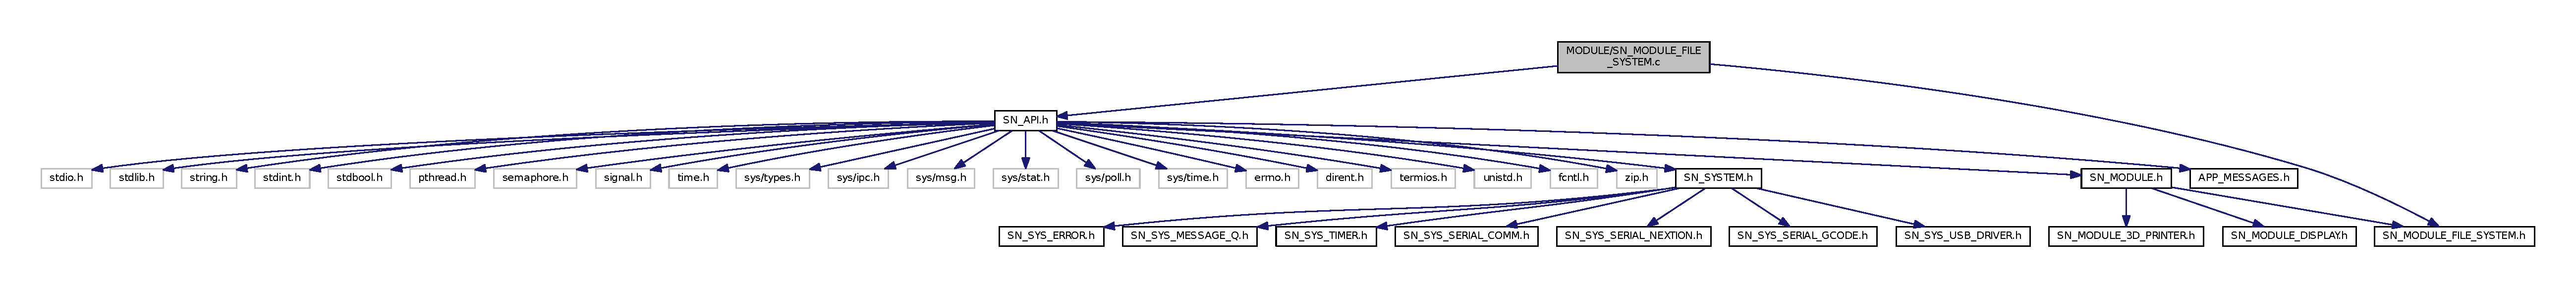
\includegraphics[width=350pt]{SN__MODULE__FILE__SYSTEM_8c__incl}
\end{center}
\end{figure}
\subsection*{Classes}
\begin{DoxyCompactItemize}
\item 
struct \hyperlink{structmoduel__file__system}{moduel\+\_\+file\+\_\+system}
\end{DoxyCompactItemize}
\subsection*{Macros}
\begin{Indent}\textbf{ File path \& name config}\par
\begin{DoxyCompactItemize}
\item 
\mbox{\Hypertarget{SN__MODULE__FILE__SYSTEM_8c_a90a97b80d1b63c85382d5776ed95c12d}\label{SN__MODULE__FILE__SYSTEM_8c_a90a97b80d1b63c85382d5776ed95c12d}} 
\#define {\bfseries F\+I\+L\+E\+N\+A\+M\+E\+\_\+\+E\+XT}~\char`\"{}cws\char`\"{}
\item 
\mbox{\Hypertarget{SN__MODULE__FILE__SYSTEM_8c_a58ef4a7f7727a62dc568ac3789c4b43e}\label{SN__MODULE__FILE__SYSTEM_8c_a58ef4a7f7727a62dc568ac3789c4b43e}} 
\#define {\bfseries I\+M\+A\+G\+E\+\_\+\+F\+I\+L\+E\+N\+A\+M\+E\+\_\+\+E\+XT}~\char`\"{}png\char`\"{}
\item 
\mbox{\Hypertarget{SN__MODULE__FILE__SYSTEM_8c_af3a37ddad69a98c185798e80a58dcbdb}\label{SN__MODULE__FILE__SYSTEM_8c_af3a37ddad69a98c185798e80a58dcbdb}} 
\#define {\bfseries C\+O\+N\+F\+I\+G\+\_\+\+F\+I\+L\+E\+N\+A\+ME}~\char`\"{}manifest\char`\"{}
\item 
\mbox{\Hypertarget{SN__MODULE__FILE__SYSTEM_8c_a33c847933de40ec5490978d29993f256}\label{SN__MODULE__FILE__SYSTEM_8c_a33c847933de40ec5490978d29993f256}} 
\#define {\bfseries C\+O\+N\+F\+I\+G\+\_\+\+F\+I\+L\+E\+N\+A\+M\+E\+\_\+\+E\+XT}~\char`\"{}xml\char`\"{}
\end{DoxyCompactItemize}
\end{Indent}
\begin{Indent}\textbf{ Z config}\par
\begin{DoxyCompactItemize}
\item 
\mbox{\Hypertarget{SN__MODULE__FILE__SYSTEM_8c_a1c0b9f2786f7fba20a129ab1147f47af}\label{SN__MODULE__FILE__SYSTEM_8c_a1c0b9f2786f7fba20a129ab1147f47af}} 
\#define {\bfseries Z\+\_\+\+D\+E\+L\+A\+Y\+\_\+\+O\+F\+F\+S\+ET}~(1600)
\item 
\#define \hyperlink{SN__MODULE__FILE__SYSTEM_8c_adf99d5fcfe3bcd52ac77e94ce4b155a4}{S\+P\+E\+E\+D\+\_\+\+M\+M\+\_\+\+M\+I\+N\+\_\+\+T\+O\+\_\+\+M\+M\+\_\+\+M\+S\+EC}(speed\+\_\+mm\+\_\+min)~((speed\+\_\+mm\+\_\+min) / (60 $\ast$ 1000))
\begin{DoxyCompactList}\small\item\em mm/m to mm/s \end{DoxyCompactList}\item 
\#define \hyperlink{SN__MODULE__FILE__SYSTEM_8c_a4ba1f76e9068f6236bcedd7660f4ae68}{Z\+\_\+\+D\+E\+L\+A\+Y\+\_\+\+M\+S\+E\+C\+\_\+\+C\+AL}(distnace,  speed)~((((distnace) $\ast$ 2) / (\hyperlink{SN__MODULE__FILE__SYSTEM_8c_adf99d5fcfe3bcd52ac77e94ce4b155a4}{S\+P\+E\+E\+D\+\_\+\+M\+M\+\_\+\+M\+I\+N\+\_\+\+T\+O\+\_\+\+M\+M\+\_\+\+M\+S\+EC}(speed))) + Z\+\_\+\+D\+E\+L\+A\+Y\+\_\+\+O\+F\+F\+S\+ET)
\begin{DoxyCompactList}\small\item\em calculate z delay \end{DoxyCompactList}\end{DoxyCompactItemize}
\end{Indent}
\begin{Indent}\textbf{ Other Define}\par
\begin{DoxyCompactItemize}
\item 
\mbox{\Hypertarget{SN__MODULE__FILE__SYSTEM_8c_a9dae37b6b57e30542ac5d55a27d6e46c}\label{SN__MODULE__FILE__SYSTEM_8c_a9dae37b6b57e30542ac5d55a27d6e46c}} 
\#define {\bfseries D\+E\+F\+A\+U\+L\+T\+\_\+\+D\+E\+V\+I\+C\+E\+\_\+\+N\+A\+ME}~\char`\"{}P\+O\+L\+A\+R\+IS 500\char`\"{}
\end{DoxyCompactItemize}
\end{Indent}
\subsection*{Typedefs}
\begin{DoxyCompactItemize}
\item 
\mbox{\Hypertarget{SN__MODULE__FILE__SYSTEM_8c_abda63c309884282ae928adea503d751e}\label{SN__MODULE__FILE__SYSTEM_8c_abda63c309884282ae928adea503d751e}} 
typedef struct \hyperlink{structmoduel__file__system}{moduel\+\_\+file\+\_\+system} {\bfseries module\+File\+System\+\_\+t}
\end{DoxyCompactItemize}
\subsection*{Enumerations}
\begin{DoxyCompactItemize}
\item 
enum \hyperlink{SN__MODULE__FILE__SYSTEM_8c_a1741329032d0063dbc7a4b3c87ca11d3}{evt\+File\+System\+\_\+t} \{ \newline
\hyperlink{SN__MODULE__FILE__SYSTEM_8c_a1741329032d0063dbc7a4b3c87ca11d3aa90a0316beef03c3f6578b9f020a3cdc}{M\+S\+G\+\_\+\+F\+I\+L\+E\+\_\+\+S\+Y\+S\+T\+E\+M\+\_\+\+U\+S\+B\+\_\+\+M\+O\+U\+NT} = 0, 
\hyperlink{SN__MODULE__FILE__SYSTEM_8c_a1741329032d0063dbc7a4b3c87ca11d3ae2d48c5d8f8d96d2cb1504e421b7006c}{M\+S\+G\+\_\+\+F\+I\+L\+E\+\_\+\+S\+Y\+S\+T\+E\+M\+\_\+\+U\+S\+B\+\_\+\+U\+N\+M\+O\+U\+NT}, 
\hyperlink{SN__MODULE__FILE__SYSTEM_8c_a1741329032d0063dbc7a4b3c87ca11d3a9fb6add4802c96906104f0f35bf20505}{M\+S\+G\+\_\+\+F\+I\+L\+E\+\_\+\+S\+Y\+S\+T\+E\+M\+\_\+\+R\+E\+AD}, 
\hyperlink{SN__MODULE__FILE__SYSTEM_8c_a1741329032d0063dbc7a4b3c87ca11d3a9cddd0942f0e11ef00914095288e3e3c}{M\+S\+G\+\_\+\+F\+I\+L\+E\+\_\+\+S\+Y\+S\+T\+E\+M\+\_\+\+U\+P\+D\+A\+TE}, 
\newline
\hyperlink{SN__MODULE__FILE__SYSTEM_8c_a1741329032d0063dbc7a4b3c87ca11d3afb2b8952e92dbf8fd8fce41f13656370}{M\+S\+G\+\_\+\+F\+I\+L\+E\+\_\+\+S\+Y\+S\+T\+E\+M\+\_\+\+W\+A\+I\+T\+I\+NG}, 
\hyperlink{SN__MODULE__FILE__SYSTEM_8c_a1741329032d0063dbc7a4b3c87ca11d3a097e5f0aeb399c3a2a096a4b7d2bc799}{M\+S\+G\+\_\+\+F\+I\+L\+E\+\_\+\+S\+Y\+S\+T\+E\+M\+\_\+\+N\+O\+NE}, 
\hyperlink{SN__MODULE__FILE__SYSTEM_8c_a1741329032d0063dbc7a4b3c87ca11d3a3f1a3f9c1b71d42b5fefa2b4f52a526a}{M\+S\+G\+\_\+\+F\+I\+L\+E\+\_\+\+S\+Y\+S\+T\+E\+M\+\_\+\+I\+G\+N\+O\+RE} = 0x\+F\+F01
 \}
\end{DoxyCompactItemize}
\subsection*{Functions}
\begin{DoxyCompactItemize}
\item 
\hyperlink{group__SYSTEM__ERROR_ga4540713b9a7a18ce44d78c3a10f7442f}{S\+N\+\_\+\+S\+T\+A\+T\+US} \hyperlink{group__MODULE__FILE__SYSTEM_gadfe4c4eeb9c662e30893824357bc46a5}{S\+N\+\_\+\+M\+O\+D\+U\+L\+E\+\_\+\+F\+I\+L\+E\+\_\+\+S\+Y\+S\+T\+E\+M\+\_\+\+Get} (\hyperlink{structfile__system}{fs\+\_\+t} $\ast$p\+Fs)
\item 
\hyperlink{group__SYSTEM__ERROR_ga4540713b9a7a18ce44d78c3a10f7442f}{S\+N\+\_\+\+S\+T\+A\+T\+US} \hyperlink{group__MODULE__FILE__SYSTEM_ga7df4490475224028341c54f5d5db5736}{S\+N\+\_\+\+M\+O\+D\+U\+L\+E\+\_\+\+F\+I\+L\+E\+\_\+\+S\+Y\+S\+T\+E\+M\+\_\+\+Update} (void)
\item 
\hyperlink{group__SYSTEM__ERROR_ga4540713b9a7a18ce44d78c3a10f7442f}{S\+N\+\_\+\+S\+T\+A\+T\+US} \hyperlink{group__MODULE__FILE__SYSTEM_ga4fba82e15bc9a77407cacaa1a6aadd50}{S\+N\+\_\+\+M\+O\+D\+U\+L\+E\+\_\+\+F\+I\+L\+E\+\_\+\+S\+Y\+S\+T\+E\+M\+\_\+\+Machine\+Info\+Init} (void)
\item 
\hyperlink{group__SYSTEM__ERROR_ga4540713b9a7a18ce44d78c3a10f7442f}{S\+N\+\_\+\+S\+T\+A\+T\+US} \hyperlink{group__MODULE__FILE__SYSTEM_gadbd5aafed31faed399abd08193a04bc8}{S\+N\+\_\+\+M\+O\+D\+U\+L\+E\+\_\+\+F\+I\+L\+E\+\_\+\+S\+Y\+S\+T\+E\+M\+\_\+\+Print\+Info\+Init} (uint32\+\_\+t page\+Index, uint32\+\_\+t item\+Index)
\item 
\hyperlink{structmachine__information}{machine\+Info\+\_\+t} \hyperlink{group__MODULE__FILE__SYSTEM_ga647e18cfc2415cb546d69b327ed76232}{S\+N\+\_\+\+M\+O\+D\+U\+L\+E\+\_\+\+F\+I\+L\+E\+\_\+\+S\+Y\+S\+T\+E\+M\+\_\+\+Machine\+Info\+Get} (void)
\item 
\hyperlink{structprint__information}{print\+Info\+\_\+t} \hyperlink{group__MODULE__FILE__SYSTEM_ga6679d04769a997531a277ba3940cf16c}{S\+N\+\_\+\+M\+O\+D\+U\+L\+E\+\_\+\+F\+I\+L\+E\+\_\+\+S\+Y\+S\+T\+E\+M\+\_\+\+Print\+Info\+Get} (void)
\item 
\hyperlink{group__SYSTEM__ERROR_ga4540713b9a7a18ce44d78c3a10f7442f}{S\+N\+\_\+\+S\+T\+A\+T\+US} \hyperlink{group__MODULE__FILE__SYSTEM_ga86125af6adcd6218d4ebdb484e11d273}{S\+N\+\_\+\+M\+O\+D\+U\+L\+E\+\_\+\+F\+I\+L\+E\+\_\+\+S\+Y\+S\+T\+E\+M\+\_\+\+Machine\+Info\+Uninit} (void)
\item 
\hyperlink{group__SYSTEM__ERROR_ga4540713b9a7a18ce44d78c3a10f7442f}{S\+N\+\_\+\+S\+T\+A\+T\+US} \hyperlink{group__MODULE__FILE__SYSTEM_gaddd6a0e37c98d7a5aba88db31875e44e}{S\+N\+\_\+\+M\+O\+D\+U\+L\+E\+\_\+\+F\+I\+L\+E\+\_\+\+S\+Y\+S\+T\+E\+M\+\_\+\+Print\+Info\+Uninit} (void)
\item 
\hyperlink{group__SYSTEM__ERROR_ga4540713b9a7a18ce44d78c3a10f7442f}{S\+N\+\_\+\+S\+T\+A\+T\+US} \hyperlink{group__MODULE__FILE__SYSTEM_ga4b8101916d7de3e4d3004b79f4c8c2de}{S\+N\+\_\+\+M\+O\+D\+U\+L\+E\+\_\+\+F\+I\+L\+E\+\_\+\+S\+Y\+S\+T\+E\+M\+\_\+\+Init} (void)
\item 
\hyperlink{group__SYSTEM__ERROR_ga4540713b9a7a18ce44d78c3a10f7442f}{S\+N\+\_\+\+S\+T\+A\+T\+US} \hyperlink{group__MODULE__FILE__SYSTEM_ga39c0e153f169cc6bdb35bce4d2a9194b}{S\+N\+\_\+\+M\+O\+D\+U\+L\+E\+\_\+\+F\+I\+L\+E\+\_\+\+S\+Y\+S\+T\+E\+M\+\_\+\+Uninit} (void)
\end{DoxyCompactItemize}


\subsection{Detailed Description}
\begin{DoxyAuthor}{Author}
Bato 
\end{DoxyAuthor}
\begin{DoxyDate}{Date}
18 Sep 2018 
\end{DoxyDate}
\begin{DoxySeeAlso}{See also}
\href{http://www.stack.nl/~dimitri/doxygen/docblocks.html}{\tt http\+://www.\+stack.\+nl/$\sim$dimitri/doxygen/docblocks.\+html} 

\href{http://www.stack.nl/~dimitri/doxygen/commands.html}{\tt http\+://www.\+stack.\+nl/$\sim$dimitri/doxygen/commands.\+html} 
\end{DoxySeeAlso}


\subsection{Macro Definition Documentation}
\mbox{\Hypertarget{SN__MODULE__FILE__SYSTEM_8c_adf99d5fcfe3bcd52ac77e94ce4b155a4}\label{SN__MODULE__FILE__SYSTEM_8c_adf99d5fcfe3bcd52ac77e94ce4b155a4}} 
\index{S\+N\+\_\+\+M\+O\+D\+U\+L\+E\+\_\+\+F\+I\+L\+E\+\_\+\+S\+Y\+S\+T\+E\+M.\+c@{S\+N\+\_\+\+M\+O\+D\+U\+L\+E\+\_\+\+F\+I\+L\+E\+\_\+\+S\+Y\+S\+T\+E\+M.\+c}!S\+P\+E\+E\+D\+\_\+\+M\+M\+\_\+\+M\+I\+N\+\_\+\+T\+O\+\_\+\+M\+M\+\_\+\+M\+S\+EC@{S\+P\+E\+E\+D\+\_\+\+M\+M\+\_\+\+M\+I\+N\+\_\+\+T\+O\+\_\+\+M\+M\+\_\+\+M\+S\+EC}}
\index{S\+P\+E\+E\+D\+\_\+\+M\+M\+\_\+\+M\+I\+N\+\_\+\+T\+O\+\_\+\+M\+M\+\_\+\+M\+S\+EC@{S\+P\+E\+E\+D\+\_\+\+M\+M\+\_\+\+M\+I\+N\+\_\+\+T\+O\+\_\+\+M\+M\+\_\+\+M\+S\+EC}!S\+N\+\_\+\+M\+O\+D\+U\+L\+E\+\_\+\+F\+I\+L\+E\+\_\+\+S\+Y\+S\+T\+E\+M.\+c@{S\+N\+\_\+\+M\+O\+D\+U\+L\+E\+\_\+\+F\+I\+L\+E\+\_\+\+S\+Y\+S\+T\+E\+M.\+c}}
\subsubsection{\texorpdfstring{S\+P\+E\+E\+D\+\_\+\+M\+M\+\_\+\+M\+I\+N\+\_\+\+T\+O\+\_\+\+M\+M\+\_\+\+M\+S\+EC}{SPEED\_MM\_MIN\_TO\_MM\_MSEC}}
{\footnotesize\ttfamily \#define S\+P\+E\+E\+D\+\_\+\+M\+M\+\_\+\+M\+I\+N\+\_\+\+T\+O\+\_\+\+M\+M\+\_\+\+M\+S\+EC(\begin{DoxyParamCaption}\item[{}]{speed\+\_\+mm\+\_\+min }\end{DoxyParamCaption})~((speed\+\_\+mm\+\_\+min) / (60 $\ast$ 1000))}



mm/m to mm/s 


\begin{DoxyParams}{Parameters}
{\em speed\+\_\+mm\+\_\+min} & \\
\hline
\end{DoxyParams}
\begin{DoxyReturn}{Returns}
mm/s 
\end{DoxyReturn}
\mbox{\Hypertarget{SN__MODULE__FILE__SYSTEM_8c_a4ba1f76e9068f6236bcedd7660f4ae68}\label{SN__MODULE__FILE__SYSTEM_8c_a4ba1f76e9068f6236bcedd7660f4ae68}} 
\index{S\+N\+\_\+\+M\+O\+D\+U\+L\+E\+\_\+\+F\+I\+L\+E\+\_\+\+S\+Y\+S\+T\+E\+M.\+c@{S\+N\+\_\+\+M\+O\+D\+U\+L\+E\+\_\+\+F\+I\+L\+E\+\_\+\+S\+Y\+S\+T\+E\+M.\+c}!Z\+\_\+\+D\+E\+L\+A\+Y\+\_\+\+M\+S\+E\+C\+\_\+\+C\+AL@{Z\+\_\+\+D\+E\+L\+A\+Y\+\_\+\+M\+S\+E\+C\+\_\+\+C\+AL}}
\index{Z\+\_\+\+D\+E\+L\+A\+Y\+\_\+\+M\+S\+E\+C\+\_\+\+C\+AL@{Z\+\_\+\+D\+E\+L\+A\+Y\+\_\+\+M\+S\+E\+C\+\_\+\+C\+AL}!S\+N\+\_\+\+M\+O\+D\+U\+L\+E\+\_\+\+F\+I\+L\+E\+\_\+\+S\+Y\+S\+T\+E\+M.\+c@{S\+N\+\_\+\+M\+O\+D\+U\+L\+E\+\_\+\+F\+I\+L\+E\+\_\+\+S\+Y\+S\+T\+E\+M.\+c}}
\subsubsection{\texorpdfstring{Z\+\_\+\+D\+E\+L\+A\+Y\+\_\+\+M\+S\+E\+C\+\_\+\+C\+AL}{Z\_DELAY\_MSEC\_CAL}}
{\footnotesize\ttfamily \#define Z\+\_\+\+D\+E\+L\+A\+Y\+\_\+\+M\+S\+E\+C\+\_\+\+C\+AL(\begin{DoxyParamCaption}\item[{}]{distnace,  }\item[{}]{speed }\end{DoxyParamCaption})~((((distnace) $\ast$ 2) / (\hyperlink{SN__MODULE__FILE__SYSTEM_8c_adf99d5fcfe3bcd52ac77e94ce4b155a4}{S\+P\+E\+E\+D\+\_\+\+M\+M\+\_\+\+M\+I\+N\+\_\+\+T\+O\+\_\+\+M\+M\+\_\+\+M\+S\+EC}(speed))) + Z\+\_\+\+D\+E\+L\+A\+Y\+\_\+\+O\+F\+F\+S\+ET)}



calculate z delay 


\begin{DoxyParams}{Parameters}
{\em distance} & \\
\hline
{\em speed} & \\
\hline
\end{DoxyParams}
\begin{DoxyReturn}{Returns}
z\+\_\+delay (msec) 
\end{DoxyReturn}


\subsection{Enumeration Type Documentation}
\mbox{\Hypertarget{SN__MODULE__FILE__SYSTEM_8c_a1741329032d0063dbc7a4b3c87ca11d3}\label{SN__MODULE__FILE__SYSTEM_8c_a1741329032d0063dbc7a4b3c87ca11d3}} 
\index{S\+N\+\_\+\+M\+O\+D\+U\+L\+E\+\_\+\+F\+I\+L\+E\+\_\+\+S\+Y\+S\+T\+E\+M.\+c@{S\+N\+\_\+\+M\+O\+D\+U\+L\+E\+\_\+\+F\+I\+L\+E\+\_\+\+S\+Y\+S\+T\+E\+M.\+c}!evt\+File\+System\+\_\+t@{evt\+File\+System\+\_\+t}}
\index{evt\+File\+System\+\_\+t@{evt\+File\+System\+\_\+t}!S\+N\+\_\+\+M\+O\+D\+U\+L\+E\+\_\+\+F\+I\+L\+E\+\_\+\+S\+Y\+S\+T\+E\+M.\+c@{S\+N\+\_\+\+M\+O\+D\+U\+L\+E\+\_\+\+F\+I\+L\+E\+\_\+\+S\+Y\+S\+T\+E\+M.\+c}}
\subsubsection{\texorpdfstring{evt\+File\+System\+\_\+t}{evtFileSystem\_t}}
{\footnotesize\ttfamily enum \hyperlink{SN__MODULE__FILE__SYSTEM_8c_a1741329032d0063dbc7a4b3c87ca11d3}{evt\+File\+System\+\_\+t}}

\begin{DoxyEnumFields}{Enumerator}
\raisebox{\heightof{T}}[0pt][0pt]{\index{M\+S\+G\+\_\+\+F\+I\+L\+E\+\_\+\+S\+Y\+S\+T\+E\+M\+\_\+\+U\+S\+B\+\_\+\+M\+O\+U\+NT@{M\+S\+G\+\_\+\+F\+I\+L\+E\+\_\+\+S\+Y\+S\+T\+E\+M\+\_\+\+U\+S\+B\+\_\+\+M\+O\+U\+NT}!S\+N\+\_\+\+M\+O\+D\+U\+L\+E\+\_\+\+F\+I\+L\+E\+\_\+\+S\+Y\+S\+T\+E\+M.\+c@{S\+N\+\_\+\+M\+O\+D\+U\+L\+E\+\_\+\+F\+I\+L\+E\+\_\+\+S\+Y\+S\+T\+E\+M.\+c}}\index{S\+N\+\_\+\+M\+O\+D\+U\+L\+E\+\_\+\+F\+I\+L\+E\+\_\+\+S\+Y\+S\+T\+E\+M.\+c@{S\+N\+\_\+\+M\+O\+D\+U\+L\+E\+\_\+\+F\+I\+L\+E\+\_\+\+S\+Y\+S\+T\+E\+M.\+c}!M\+S\+G\+\_\+\+F\+I\+L\+E\+\_\+\+S\+Y\+S\+T\+E\+M\+\_\+\+U\+S\+B\+\_\+\+M\+O\+U\+NT@{M\+S\+G\+\_\+\+F\+I\+L\+E\+\_\+\+S\+Y\+S\+T\+E\+M\+\_\+\+U\+S\+B\+\_\+\+M\+O\+U\+NT}}}\mbox{\Hypertarget{SN__MODULE__FILE__SYSTEM_8c_a1741329032d0063dbc7a4b3c87ca11d3aa90a0316beef03c3f6578b9f020a3cdc}\label{SN__MODULE__FILE__SYSTEM_8c_a1741329032d0063dbc7a4b3c87ca11d3aa90a0316beef03c3f6578b9f020a3cdc}} 
M\+S\+G\+\_\+\+F\+I\+L\+E\+\_\+\+S\+Y\+S\+T\+E\+M\+\_\+\+U\+S\+B\+\_\+\+M\+O\+U\+NT&U\+SB Mount \\
\hline

\raisebox{\heightof{T}}[0pt][0pt]{\index{M\+S\+G\+\_\+\+F\+I\+L\+E\+\_\+\+S\+Y\+S\+T\+E\+M\+\_\+\+U\+S\+B\+\_\+\+U\+N\+M\+O\+U\+NT@{M\+S\+G\+\_\+\+F\+I\+L\+E\+\_\+\+S\+Y\+S\+T\+E\+M\+\_\+\+U\+S\+B\+\_\+\+U\+N\+M\+O\+U\+NT}!S\+N\+\_\+\+M\+O\+D\+U\+L\+E\+\_\+\+F\+I\+L\+E\+\_\+\+S\+Y\+S\+T\+E\+M.\+c@{S\+N\+\_\+\+M\+O\+D\+U\+L\+E\+\_\+\+F\+I\+L\+E\+\_\+\+S\+Y\+S\+T\+E\+M.\+c}}\index{S\+N\+\_\+\+M\+O\+D\+U\+L\+E\+\_\+\+F\+I\+L\+E\+\_\+\+S\+Y\+S\+T\+E\+M.\+c@{S\+N\+\_\+\+M\+O\+D\+U\+L\+E\+\_\+\+F\+I\+L\+E\+\_\+\+S\+Y\+S\+T\+E\+M.\+c}!M\+S\+G\+\_\+\+F\+I\+L\+E\+\_\+\+S\+Y\+S\+T\+E\+M\+\_\+\+U\+S\+B\+\_\+\+U\+N\+M\+O\+U\+NT@{M\+S\+G\+\_\+\+F\+I\+L\+E\+\_\+\+S\+Y\+S\+T\+E\+M\+\_\+\+U\+S\+B\+\_\+\+U\+N\+M\+O\+U\+NT}}}\mbox{\Hypertarget{SN__MODULE__FILE__SYSTEM_8c_a1741329032d0063dbc7a4b3c87ca11d3ae2d48c5d8f8d96d2cb1504e421b7006c}\label{SN__MODULE__FILE__SYSTEM_8c_a1741329032d0063dbc7a4b3c87ca11d3ae2d48c5d8f8d96d2cb1504e421b7006c}} 
M\+S\+G\+\_\+\+F\+I\+L\+E\+\_\+\+S\+Y\+S\+T\+E\+M\+\_\+\+U\+S\+B\+\_\+\+U\+N\+M\+O\+U\+NT&U\+SB Unmount \\
\hline

\raisebox{\heightof{T}}[0pt][0pt]{\index{M\+S\+G\+\_\+\+F\+I\+L\+E\+\_\+\+S\+Y\+S\+T\+E\+M\+\_\+\+R\+E\+AD@{M\+S\+G\+\_\+\+F\+I\+L\+E\+\_\+\+S\+Y\+S\+T\+E\+M\+\_\+\+R\+E\+AD}!S\+N\+\_\+\+M\+O\+D\+U\+L\+E\+\_\+\+F\+I\+L\+E\+\_\+\+S\+Y\+S\+T\+E\+M.\+c@{S\+N\+\_\+\+M\+O\+D\+U\+L\+E\+\_\+\+F\+I\+L\+E\+\_\+\+S\+Y\+S\+T\+E\+M.\+c}}\index{S\+N\+\_\+\+M\+O\+D\+U\+L\+E\+\_\+\+F\+I\+L\+E\+\_\+\+S\+Y\+S\+T\+E\+M.\+c@{S\+N\+\_\+\+M\+O\+D\+U\+L\+E\+\_\+\+F\+I\+L\+E\+\_\+\+S\+Y\+S\+T\+E\+M.\+c}!M\+S\+G\+\_\+\+F\+I\+L\+E\+\_\+\+S\+Y\+S\+T\+E\+M\+\_\+\+R\+E\+AD@{M\+S\+G\+\_\+\+F\+I\+L\+E\+\_\+\+S\+Y\+S\+T\+E\+M\+\_\+\+R\+E\+AD}}}\mbox{\Hypertarget{SN__MODULE__FILE__SYSTEM_8c_a1741329032d0063dbc7a4b3c87ca11d3a9fb6add4802c96906104f0f35bf20505}\label{SN__MODULE__FILE__SYSTEM_8c_a1741329032d0063dbc7a4b3c87ca11d3a9fb6add4802c96906104f0f35bf20505}} 
M\+S\+G\+\_\+\+F\+I\+L\+E\+\_\+\+S\+Y\+S\+T\+E\+M\+\_\+\+R\+E\+AD&Read U\+SB -\/ when U\+SB Mounted \\
\hline

\raisebox{\heightof{T}}[0pt][0pt]{\index{M\+S\+G\+\_\+\+F\+I\+L\+E\+\_\+\+S\+Y\+S\+T\+E\+M\+\_\+\+U\+P\+D\+A\+TE@{M\+S\+G\+\_\+\+F\+I\+L\+E\+\_\+\+S\+Y\+S\+T\+E\+M\+\_\+\+U\+P\+D\+A\+TE}!S\+N\+\_\+\+M\+O\+D\+U\+L\+E\+\_\+\+F\+I\+L\+E\+\_\+\+S\+Y\+S\+T\+E\+M.\+c@{S\+N\+\_\+\+M\+O\+D\+U\+L\+E\+\_\+\+F\+I\+L\+E\+\_\+\+S\+Y\+S\+T\+E\+M.\+c}}\index{S\+N\+\_\+\+M\+O\+D\+U\+L\+E\+\_\+\+F\+I\+L\+E\+\_\+\+S\+Y\+S\+T\+E\+M.\+c@{S\+N\+\_\+\+M\+O\+D\+U\+L\+E\+\_\+\+F\+I\+L\+E\+\_\+\+S\+Y\+S\+T\+E\+M.\+c}!M\+S\+G\+\_\+\+F\+I\+L\+E\+\_\+\+S\+Y\+S\+T\+E\+M\+\_\+\+U\+P\+D\+A\+TE@{M\+S\+G\+\_\+\+F\+I\+L\+E\+\_\+\+S\+Y\+S\+T\+E\+M\+\_\+\+U\+P\+D\+A\+TE}}}\mbox{\Hypertarget{SN__MODULE__FILE__SYSTEM_8c_a1741329032d0063dbc7a4b3c87ca11d3a9cddd0942f0e11ef00914095288e3e3c}\label{SN__MODULE__FILE__SYSTEM_8c_a1741329032d0063dbc7a4b3c87ca11d3a9cddd0942f0e11ef00914095288e3e3c}} 
M\+S\+G\+\_\+\+F\+I\+L\+E\+\_\+\+S\+Y\+S\+T\+E\+M\+\_\+\+U\+P\+D\+A\+TE&Update File System -\/ when read U\+SB Finish \\
\hline

\raisebox{\heightof{T}}[0pt][0pt]{\index{M\+S\+G\+\_\+\+F\+I\+L\+E\+\_\+\+S\+Y\+S\+T\+E\+M\+\_\+\+W\+A\+I\+T\+I\+NG@{M\+S\+G\+\_\+\+F\+I\+L\+E\+\_\+\+S\+Y\+S\+T\+E\+M\+\_\+\+W\+A\+I\+T\+I\+NG}!S\+N\+\_\+\+M\+O\+D\+U\+L\+E\+\_\+\+F\+I\+L\+E\+\_\+\+S\+Y\+S\+T\+E\+M.\+c@{S\+N\+\_\+\+M\+O\+D\+U\+L\+E\+\_\+\+F\+I\+L\+E\+\_\+\+S\+Y\+S\+T\+E\+M.\+c}}\index{S\+N\+\_\+\+M\+O\+D\+U\+L\+E\+\_\+\+F\+I\+L\+E\+\_\+\+S\+Y\+S\+T\+E\+M.\+c@{S\+N\+\_\+\+M\+O\+D\+U\+L\+E\+\_\+\+F\+I\+L\+E\+\_\+\+S\+Y\+S\+T\+E\+M.\+c}!M\+S\+G\+\_\+\+F\+I\+L\+E\+\_\+\+S\+Y\+S\+T\+E\+M\+\_\+\+W\+A\+I\+T\+I\+NG@{M\+S\+G\+\_\+\+F\+I\+L\+E\+\_\+\+S\+Y\+S\+T\+E\+M\+\_\+\+W\+A\+I\+T\+I\+NG}}}\mbox{\Hypertarget{SN__MODULE__FILE__SYSTEM_8c_a1741329032d0063dbc7a4b3c87ca11d3afb2b8952e92dbf8fd8fce41f13656370}\label{SN__MODULE__FILE__SYSTEM_8c_a1741329032d0063dbc7a4b3c87ca11d3afb2b8952e92dbf8fd8fce41f13656370}} 
M\+S\+G\+\_\+\+F\+I\+L\+E\+\_\+\+S\+Y\+S\+T\+E\+M\+\_\+\+W\+A\+I\+T\+I\+NG&Waiting Next Event \\
\hline

\raisebox{\heightof{T}}[0pt][0pt]{\index{M\+S\+G\+\_\+\+F\+I\+L\+E\+\_\+\+S\+Y\+S\+T\+E\+M\+\_\+\+N\+O\+NE@{M\+S\+G\+\_\+\+F\+I\+L\+E\+\_\+\+S\+Y\+S\+T\+E\+M\+\_\+\+N\+O\+NE}!S\+N\+\_\+\+M\+O\+D\+U\+L\+E\+\_\+\+F\+I\+L\+E\+\_\+\+S\+Y\+S\+T\+E\+M.\+c@{S\+N\+\_\+\+M\+O\+D\+U\+L\+E\+\_\+\+F\+I\+L\+E\+\_\+\+S\+Y\+S\+T\+E\+M.\+c}}\index{S\+N\+\_\+\+M\+O\+D\+U\+L\+E\+\_\+\+F\+I\+L\+E\+\_\+\+S\+Y\+S\+T\+E\+M.\+c@{S\+N\+\_\+\+M\+O\+D\+U\+L\+E\+\_\+\+F\+I\+L\+E\+\_\+\+S\+Y\+S\+T\+E\+M.\+c}!M\+S\+G\+\_\+\+F\+I\+L\+E\+\_\+\+S\+Y\+S\+T\+E\+M\+\_\+\+N\+O\+NE@{M\+S\+G\+\_\+\+F\+I\+L\+E\+\_\+\+S\+Y\+S\+T\+E\+M\+\_\+\+N\+O\+NE}}}\mbox{\Hypertarget{SN__MODULE__FILE__SYSTEM_8c_a1741329032d0063dbc7a4b3c87ca11d3a097e5f0aeb399c3a2a096a4b7d2bc799}\label{SN__MODULE__FILE__SYSTEM_8c_a1741329032d0063dbc7a4b3c87ca11d3a097e5f0aeb399c3a2a096a4b7d2bc799}} 
M\+S\+G\+\_\+\+F\+I\+L\+E\+\_\+\+S\+Y\+S\+T\+E\+M\+\_\+\+N\+O\+NE&B\+AD A\+C\+C\+E\+SS \\
\hline

\raisebox{\heightof{T}}[0pt][0pt]{\index{M\+S\+G\+\_\+\+F\+I\+L\+E\+\_\+\+S\+Y\+S\+T\+E\+M\+\_\+\+I\+G\+N\+O\+RE@{M\+S\+G\+\_\+\+F\+I\+L\+E\+\_\+\+S\+Y\+S\+T\+E\+M\+\_\+\+I\+G\+N\+O\+RE}!S\+N\+\_\+\+M\+O\+D\+U\+L\+E\+\_\+\+F\+I\+L\+E\+\_\+\+S\+Y\+S\+T\+E\+M.\+c@{S\+N\+\_\+\+M\+O\+D\+U\+L\+E\+\_\+\+F\+I\+L\+E\+\_\+\+S\+Y\+S\+T\+E\+M.\+c}}\index{S\+N\+\_\+\+M\+O\+D\+U\+L\+E\+\_\+\+F\+I\+L\+E\+\_\+\+S\+Y\+S\+T\+E\+M.\+c@{S\+N\+\_\+\+M\+O\+D\+U\+L\+E\+\_\+\+F\+I\+L\+E\+\_\+\+S\+Y\+S\+T\+E\+M.\+c}!M\+S\+G\+\_\+\+F\+I\+L\+E\+\_\+\+S\+Y\+S\+T\+E\+M\+\_\+\+I\+G\+N\+O\+RE@{M\+S\+G\+\_\+\+F\+I\+L\+E\+\_\+\+S\+Y\+S\+T\+E\+M\+\_\+\+I\+G\+N\+O\+RE}}}\mbox{\Hypertarget{SN__MODULE__FILE__SYSTEM_8c_a1741329032d0063dbc7a4b3c87ca11d3a3f1a3f9c1b71d42b5fefa2b4f52a526a}\label{SN__MODULE__FILE__SYSTEM_8c_a1741329032d0063dbc7a4b3c87ca11d3a3f1a3f9c1b71d42b5fefa2b4f52a526a}} 
M\+S\+G\+\_\+\+F\+I\+L\+E\+\_\+\+S\+Y\+S\+T\+E\+M\+\_\+\+I\+G\+N\+O\+RE&Came From Timer -\/ Don\textquotesingle{}t Care \\
\hline

\end{DoxyEnumFields}


���}	� �
����DEV��INO��SYN��SV~�#`�#`��#`�k��O�I]�[��

���}	� �
����DEV��INO��SYN��SV~�#`
#`
�#`
k����I]�[s 
\hypertarget{SN__SYS__MESSAGE__Q_8h}{}\section{S\+Y\+S\+T\+E\+M/\+I\+N\+C\+L\+U\+D\+E/\+S\+N\+\_\+\+S\+Y\+S\+\_\+\+M\+E\+S\+S\+A\+G\+E\+\_\+Q.h File Reference}
\label{SN__SYS__MESSAGE__Q_8h}\index{S\+Y\+S\+T\+E\+M/\+I\+N\+C\+L\+U\+D\+E/\+S\+N\+\_\+\+S\+Y\+S\+\_\+\+M\+E\+S\+S\+A\+G\+E\+\_\+\+Q.\+h@{S\+Y\+S\+T\+E\+M/\+I\+N\+C\+L\+U\+D\+E/\+S\+N\+\_\+\+S\+Y\+S\+\_\+\+M\+E\+S\+S\+A\+G\+E\+\_\+\+Q.\+h}}
This graph shows which files directly or indirectly include this file\+:\nopagebreak
\begin{figure}[H]
\begin{center}
\leavevmode
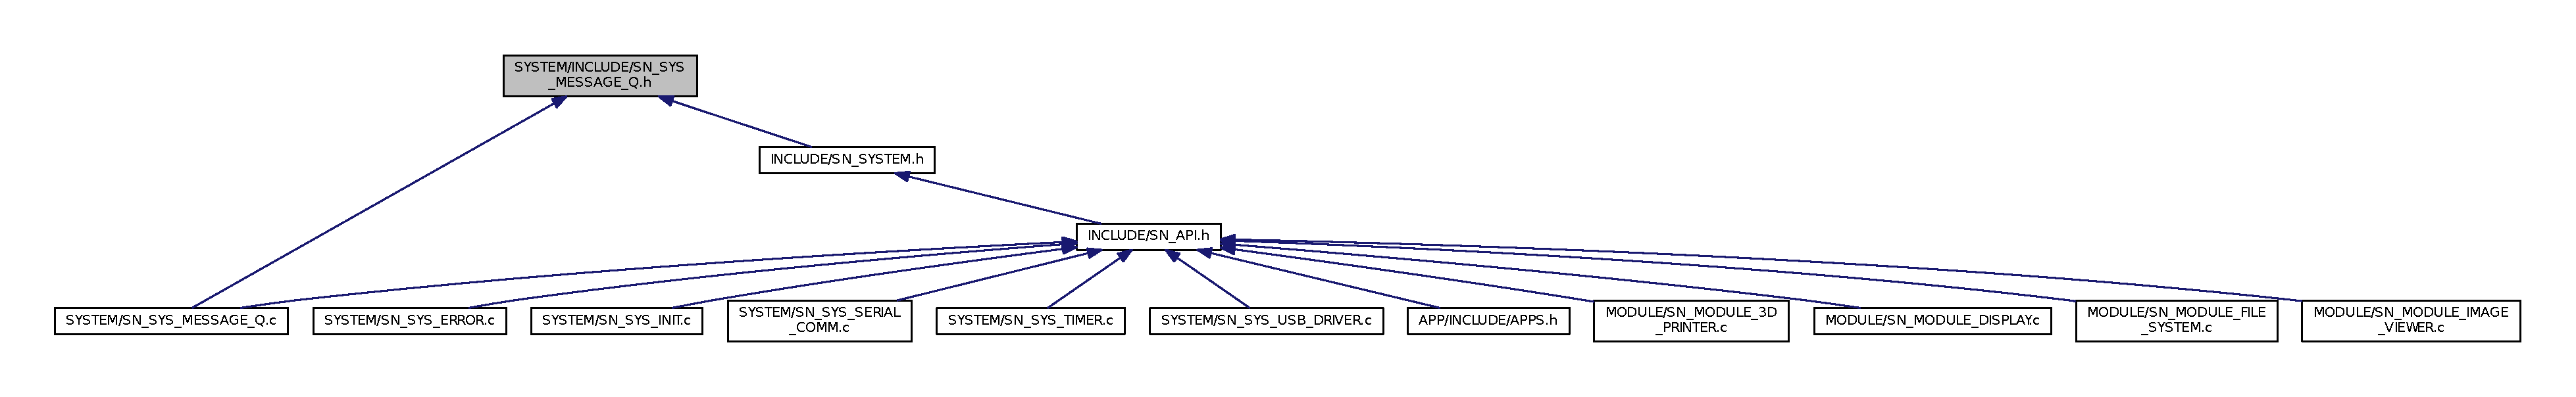
\includegraphics[width=350pt]{SN__SYS__MESSAGE__Q_8h__dep__incl}
\end{center}
\end{figure}
\subsection*{Classes}
\begin{DoxyCompactItemize}
\item 
struct \hyperlink{structgeneral__event__header}{general\+\_\+event\+\_\+header}
\item 
struct \hyperlink{structgeneral__event}{general\+\_\+event}
\item 
struct \hyperlink{structsys__message__queue}{sys\+\_\+message\+\_\+queue}
\end{DoxyCompactItemize}
\subsection*{Typedefs}
\begin{DoxyCompactItemize}
\item 
typedef uint32\+\_\+t {\bfseries event\+\_\+id\+\_\+t}
\item 
typedef uint32\+\_\+t {\bfseries event\+\_\+msg\+\_\+t}
\item 
typedef struct \hyperlink{structgeneral__event__header}{general\+\_\+event\+\_\+header} {\bfseries general\+\_\+evt\+\_\+header\+\_\+t}
\item 
typedef struct \hyperlink{structgeneral__event}{general\+\_\+event} {\bfseries general\+\_\+evt\+\_\+t}
\item 
typedef struct \hyperlink{structsys__message__queue}{sys\+\_\+message\+\_\+queue} {\bfseries sys\+Message\+Q\+Id}
\end{DoxyCompactItemize}
\subsection*{Functions}
\begin{Indent}\textbf{ System Message Queue}\par
{\em Description of Message Queue Init and Uninit funtions. }\begin{DoxyCompactItemize}
\item 
\hyperlink{group__SYSTEM__ERROR_ga4540713b9a7a18ce44d78c3a10f7442f}{S\+N\+\_\+\+S\+T\+A\+T\+US} \hyperlink{group__SYSTEM__MESSAGE__Q_ga35e9ff084626dfccd36d098827638a0c}{S\+N\+\_\+\+S\+Y\+S\+\_\+\+Message\+Q\+Init} (\hyperlink{structsys__message__queue}{sys\+Message\+Q\+Id} $\ast$msg\+Q\+Id)
\item 
\hyperlink{group__SYSTEM__ERROR_ga4540713b9a7a18ce44d78c3a10f7442f}{S\+N\+\_\+\+S\+T\+A\+T\+US} \hyperlink{group__SYSTEM__MESSAGE__Q_ga293a77ea597b70f3f2f38b919f93497e}{S\+N\+\_\+\+S\+Y\+S\+\_\+\+Message\+Q\+Remove} (\hyperlink{structsys__message__queue}{sys\+Message\+Q\+Id} $\ast$msg\+Q\+Id)
\end{DoxyCompactItemize}
\end{Indent}
\begin{Indent}\textbf{ System Message Queue \+:\+: Send \& Receive Message}\par
{\em Description of Message Queue Init and Uninit funtions. }\begin{DoxyCompactItemize}
\item 
\hyperlink{group__SYSTEM__ERROR_ga4540713b9a7a18ce44d78c3a10f7442f}{S\+N\+\_\+\+S\+T\+A\+T\+US} \hyperlink{group__SYSTEM__MESSAGE__Q_ga36e115419d4cbbfe4a6bde6e3fecf180}{S\+N\+\_\+\+S\+Y\+S\+\_\+\+Message\+Put} (\hyperlink{structsys__message__queue}{sys\+Message\+Q\+Id} $\ast$msg\+Q\+Id, event\+\_\+id\+\_\+t evt\+Id, event\+\_\+msg\+\_\+t evt\+Message)
\item 
\hyperlink{structgeneral__event}{general\+\_\+evt\+\_\+t} \hyperlink{group__SYSTEM__MESSAGE__Q_gafb2da611b3c93f1f906109e7737d67cf}{S\+N\+\_\+\+S\+Y\+S\+\_\+\+Message\+Get} (\hyperlink{structsys__message__queue}{sys\+Message\+Q\+Id} $\ast$msg\+Q\+Id)
\end{DoxyCompactItemize}
\end{Indent}


\subsection{Detailed Description}
\begin{DoxyAuthor}{Author}
Bato 
\end{DoxyAuthor}
\begin{DoxyDate}{Date}
16 Oct 2018 
\end{DoxyDate}
\begin{DoxySeeAlso}{See also}
\href{http://www.stack.nl/~dimitri/doxygen/docblocks.html}{\tt http\+://www.\+stack.\+nl/$\sim$dimitri/doxygen/docblocks.\+html} 

\href{http://www.stack.nl/~dimitri/doxygen/commands.html}{\tt http\+://www.\+stack.\+nl/$\sim$dimitri/doxygen/commands.\+html} 
\end{DoxySeeAlso}

\hypertarget{SN__SYS__SERIAL__COMM_8h}{}\section{S\+Y\+S\+T\+E\+M/\+I\+N\+C\+L\+U\+D\+E/\+S\+N\+\_\+\+S\+Y\+S\+\_\+\+S\+E\+R\+I\+A\+L\+\_\+\+C\+O\+MM.h File Reference}
\label{SN__SYS__SERIAL__COMM_8h}\index{S\+Y\+S\+T\+E\+M/\+I\+N\+C\+L\+U\+D\+E/\+S\+N\+\_\+\+S\+Y\+S\+\_\+\+S\+E\+R\+I\+A\+L\+\_\+\+C\+O\+M\+M.\+h@{S\+Y\+S\+T\+E\+M/\+I\+N\+C\+L\+U\+D\+E/\+S\+N\+\_\+\+S\+Y\+S\+\_\+\+S\+E\+R\+I\+A\+L\+\_\+\+C\+O\+M\+M.\+h}}
This graph shows which files directly or indirectly include this file\+:
\nopagebreak
\begin{figure}[H]
\begin{center}
\leavevmode
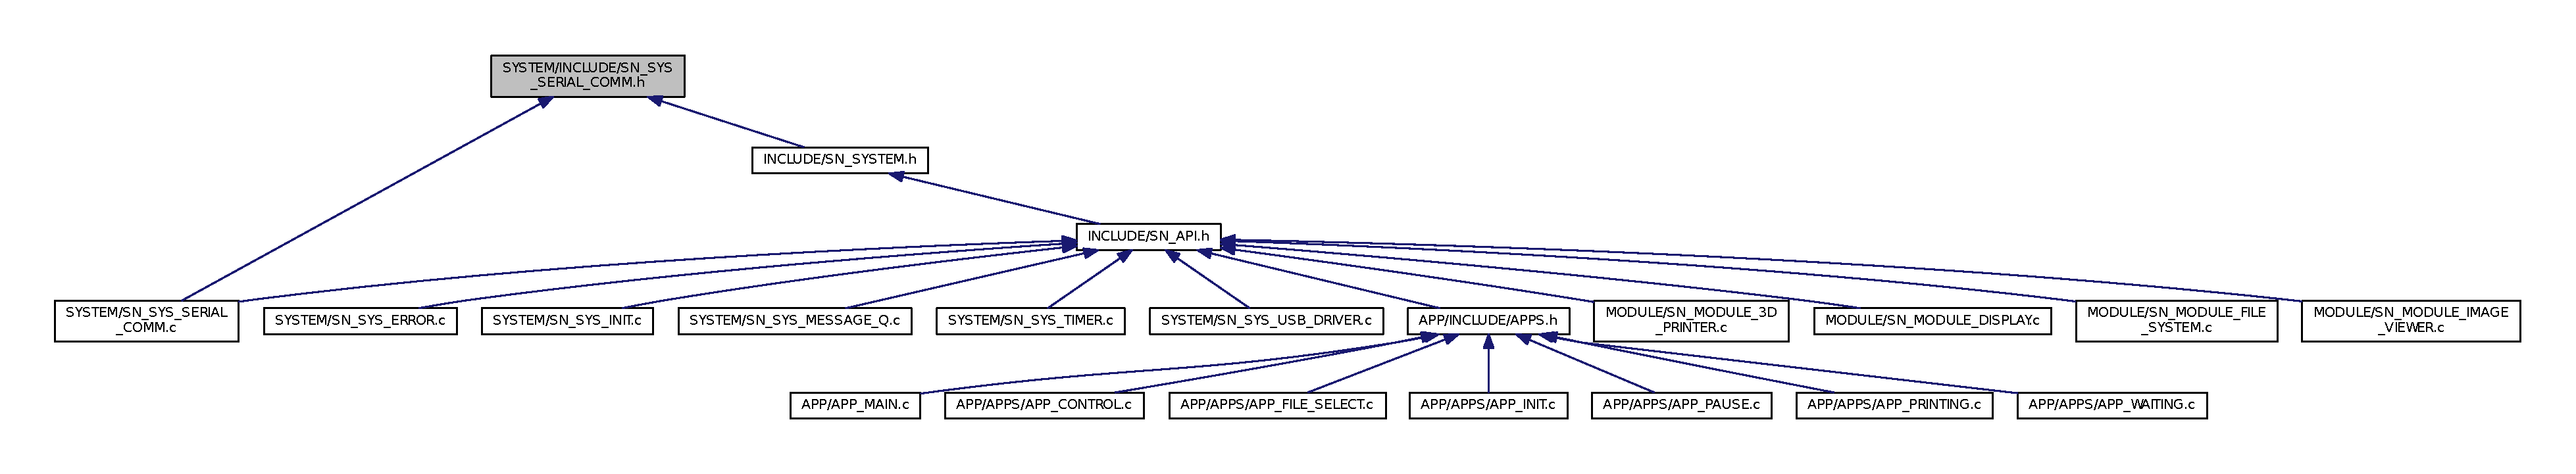
\includegraphics[width=350pt]{SN__SYS__SERIAL__COMM_8h__dep__incl}
\end{center}
\end{figure}
\subsection*{Classes}
\begin{DoxyCompactItemize}
\item 
struct \hyperlink{structsys__serial__stat}{sys\+\_\+serial\+\_\+stat}
\item 
struct \hyperlink{structsys__serial__def}{sys\+\_\+serial\+\_\+def}
\item 
struct \hyperlink{structsys__serial__id}{sys\+\_\+serial\+\_\+id}
\item 
struct \hyperlink{structsys__serial__q}{sys\+\_\+serial\+\_\+q}
\end{DoxyCompactItemize}
\subsection*{Macros}
\begin{DoxyCompactItemize}
\item 
\#define \hyperlink{group__SYSTEM__SERIAL__COMM_gab19b7880962ae52d90f784158f56f9f5}{M\+A\+X\+\_\+\+N\+U\+M\+\_\+\+O\+F\+\_\+\+S\+E\+R\+I\+AL}~4
\item 
\#define \hyperlink{group__SYSTEM__SERIAL__COMM_ga0e2406f7554f78b285eaccd1513fe392}{sys\+Serial\+Def}(name,  device,  oflags,  baud\+Rate,  rx\+Byte\+Size,  rx\+Return\+Mode)
\begin{DoxyCompactList}\small\item\em def Serial def serial for get Serial\+Id \end{DoxyCompactList}\item 
\#define {\bfseries sys\+Serial\+Thread\+Funcdef}(num)
\item 
\#define {\bfseries sys\+Serial}(name)~(\&sys\+\_\+serial\+\_\+def\+\_\+\#\#name)
\item 
\#define {\bfseries sys\+Serial\+Thread\+Func}(num)~(s\+Serial\+Thread\+\_\+\#\#num)
\item 
\#define \hyperlink{group__SYSTEM__SERIAL__COMM_ga8ef896af26917008892ad9f98480cced}{S\+N\+\_\+\+S\+Y\+S\+\_\+\+S\+E\+R\+I\+A\+L\+\_\+\+C\+O\+M\+M\+\_\+\+B\+A\+U\+D\+\_\+\+R\+A\+T\+E\+\_\+9600}~B9600
\item 
\#define {\bfseries S\+N\+\_\+\+S\+Y\+S\+\_\+\+S\+E\+R\+I\+A\+L\+\_\+\+C\+O\+M\+M\+\_\+\+B\+A\+U\+D\+\_\+\+R\+A\+T\+E\+\_\+19200}~B19200
\item 
\#define {\bfseries S\+N\+\_\+\+S\+Y\+S\+\_\+\+S\+E\+R\+I\+A\+L\+\_\+\+C\+O\+M\+M\+\_\+\+B\+A\+U\+D\+\_\+\+R\+A\+T\+E\+\_\+115200}~B115200
\item 
\#define \hyperlink{group__SYSTEM__SERIAL__COMM_ga45345dabcfb671abba160a3dac350670}{S\+N\+\_\+\+S\+Y\+S\+\_\+\+S\+E\+R\+I\+A\+L\+\_\+\+C\+O\+M\+M\+\_\+\+R\+X\+\_\+\+R\+E\+A\+L\+T\+I\+ME}~0
\item 
\#define \hyperlink{group__SYSTEM__SERIAL__COMM_ga20e8092429292afa4348544ee9fafec3}{S\+N\+\_\+\+S\+Y\+S\+\_\+\+S\+E\+R\+I\+A\+L\+\_\+\+C\+O\+M\+M\+\_\+\+R\+X\+\_\+\+B\+Y\+T\+E\+\_\+4}~4
\item 
\#define \hyperlink{group__SYSTEM__SERIAL__COMM_gaeeb374cea7f99086bd693aa158af8dc8}{S\+N\+\_\+\+S\+Y\+S\+\_\+\+S\+E\+R\+I\+A\+L\+\_\+\+C\+O\+M\+M\+\_\+\+R\+X\+\_\+\+B\+Y\+T\+E\+\_\+8}~8
\item 
\#define \hyperlink{group__SYSTEM__SERIAL__COMM_ga56161a71858040bee49e45caeb42787a}{S\+N\+\_\+\+S\+Y\+S\+\_\+\+S\+E\+R\+I\+A\+L\+\_\+\+C\+O\+M\+M\+\_\+\+R\+X\+\_\+\+B\+Y\+T\+E\+\_\+16}~16
\item 
\#define \hyperlink{group__SYSTEM__SERIAL__COMM_ga532ba920d82c8b8bf35997df3c732d4c}{S\+N\+\_\+\+S\+Y\+S\+\_\+\+S\+E\+R\+I\+A\+L\+\_\+\+C\+O\+M\+M\+\_\+\+R\+X\+\_\+\+B\+Y\+T\+E\+\_\+32}~32
\item 
\#define {\bfseries S\+N\+\_\+\+S\+Y\+S\+\_\+\+S\+E\+R\+I\+A\+L\+\_\+\+C\+O\+M\+M\+\_\+\+T\+X\+\_\+\+R\+E\+T\+U\+RN}~0
\item 
\#define {\bfseries S\+N\+\_\+\+S\+Y\+S\+\_\+\+S\+E\+R\+I\+A\+L\+\_\+\+C\+O\+M\+M\+\_\+\+T\+X\+\_\+\+C\+A\+R\+R\+I\+A\+G\+E\+\_\+\+R\+E\+T\+U\+RN}~1
\item 
\#define {\bfseries S\+N\+\_\+\+S\+Y\+S\+\_\+\+S\+E\+R\+I\+A\+L\+\_\+\+C\+O\+M\+M\+\_\+\+T\+X\+\_\+\+N\+E\+W\+\_\+\+L\+I\+N\+E\+\_\+\+R\+E\+T\+U\+RN}~2
\item 
\#define {\bfseries S\+N\+\_\+\+S\+Y\+S\+\_\+\+S\+E\+R\+I\+A\+L\+\_\+\+C\+O\+M\+M\+\_\+\+T\+X\+\_\+\+N\+X\+\_\+\+R\+E\+T\+U\+RN}~3
\item 
\#define {\bfseries S\+N\+\_\+\+S\+Y\+S\+\_\+\+S\+E\+R\+I\+A\+L\+\_\+\+C\+O\+M\+M\+\_\+\+B\+U\+F\+F\+E\+R\+\_\+\+S\+I\+ZE}~255
\item 
\#define \hyperlink{group__SYSTEM__SERIAL__COMM_gab3cb3e808e6aa6d23c73d7687b3b937e}{S\+N\+\_\+\+S\+Y\+S\+\_\+\+S\+E\+R\+I\+A\+L\+\_\+\+C\+O\+M\+M\+\_\+\+I\+N\+V\+A\+I\+L\+D\+\_\+\+U\+A\+R\+T\+\_\+\+ID}~(-\/1)
\item 
\#define \hyperlink{group__SYSTEM__SERIAL__COMM_ga3b81478c7058ceb6ed610ce8e2ca3822}{C\+A\+R\+R\+I\+A\+G\+E\+\_\+\+R\+E\+T\+U\+RN}~\char`\"{}\textbackslash{}r\char`\"{}
\item 
\#define {\bfseries N\+E\+W\+\_\+\+L\+I\+N\+E\+\_\+\+R\+E\+T\+U\+RN}~\char`\"{}\textbackslash{}n\char`\"{}
\item 
\#define {\bfseries N\+X\+\_\+\+R\+E\+T\+U\+RN}~0x\+FF
\item 
\#define {\bfseries R\+E\+T\+U\+R\+N\+\_\+\+S\+I\+ZE}~1
\end{DoxyCompactItemize}
\subsection*{Typedefs}
\begin{DoxyCompactItemize}
\item 
typedef struct \hyperlink{structsys__serial__stat}{sys\+\_\+serial\+\_\+stat} {\bfseries sys\+Serial\+Stat\+\_\+t}
\item 
typedef struct \hyperlink{structsys__serial__def}{sys\+\_\+serial\+\_\+def} {\bfseries sys\+Serial\+Def\+\_\+t}
\item 
typedef struct \hyperlink{structsys__serial__id}{sys\+\_\+serial\+\_\+id} $\ast$ {\bfseries sys\+Serial\+Id}
\item 
typedef struct \hyperlink{structsys__serial__q}{sys\+\_\+serial\+\_\+q} {\bfseries sys\+SerialQ}
\end{DoxyCompactItemize}
\subsection*{Functions}
\begin{DoxyCompactItemize}
\item 
int \hyperlink{group__SYSTEM__SERIAL__COMM_ga5945cfb2c1d87d3fa9ad40bf928bd05a}{S\+N\+\_\+\+S\+Y\+S\+\_\+\+Serial\+Init} (void)
\item 
\hyperlink{structsys__serial__id}{sys\+Serial\+Id} {\bfseries S\+N\+\_\+\+S\+Y\+S\+\_\+\+Serial\+Create} (const \hyperlink{structsys__serial__def}{sys\+Serial\+Def\+\_\+t} $\ast$serial\+Def, void $\ast$($\ast$pf\+Call\+Back)(char $\ast$))
\item 
\hyperlink{group__SYSTEM__ERROR_ga4540713b9a7a18ce44d78c3a10f7442f}{S\+N\+\_\+\+S\+T\+A\+T\+US} {\bfseries S\+N\+\_\+\+S\+Y\+S\+\_\+\+Serial\+Remove} (\hyperlink{structsys__serial__id}{sys\+Serial\+Id} serial\+Id)
\item 
int {\bfseries S\+N\+\_\+\+S\+Y\+S\+\_\+\+Serial\+Tx} (\hyperlink{structsys__serial__id}{sys\+Serial\+Id} serial\+Id, char $\ast$buffer, size\+\_\+t buffer\+Size)
\end{DoxyCompactItemize}


\subsection{Detailed Description}
\begin{DoxyAuthor}{Author}
Bato 
\end{DoxyAuthor}
\begin{DoxyDate}{Date}
18 Sep 2018 
\end{DoxyDate}
\begin{DoxySeeAlso}{See also}
\href{http://www.stack.nl/~dimitri/doxygen/docblocks.html}{\tt http\+://www.\+stack.\+nl/$\sim$dimitri/doxygen/docblocks.\+html} 

\href{http://www.stack.nl/~dimitri/doxygen/commands.html}{\tt http\+://www.\+stack.\+nl/$\sim$dimitri/doxygen/commands.\+html} 
\end{DoxySeeAlso}

\hypertarget{SN__SYS__TIMER_8h}{}\section{S\+Y\+S\+T\+E\+M/\+I\+N\+C\+L\+U\+D\+E/\+S\+N\+\_\+\+S\+Y\+S\+\_\+\+T\+I\+M\+ER.h File Reference}
\label{SN__SYS__TIMER_8h}\index{S\+Y\+S\+T\+E\+M/\+I\+N\+C\+L\+U\+D\+E/\+S\+N\+\_\+\+S\+Y\+S\+\_\+\+T\+I\+M\+E\+R.\+h@{S\+Y\+S\+T\+E\+M/\+I\+N\+C\+L\+U\+D\+E/\+S\+N\+\_\+\+S\+Y\+S\+\_\+\+T\+I\+M\+E\+R.\+h}}
This graph shows which files directly or indirectly include this file\+:
\nopagebreak
\begin{figure}[H]
\begin{center}
\leavevmode
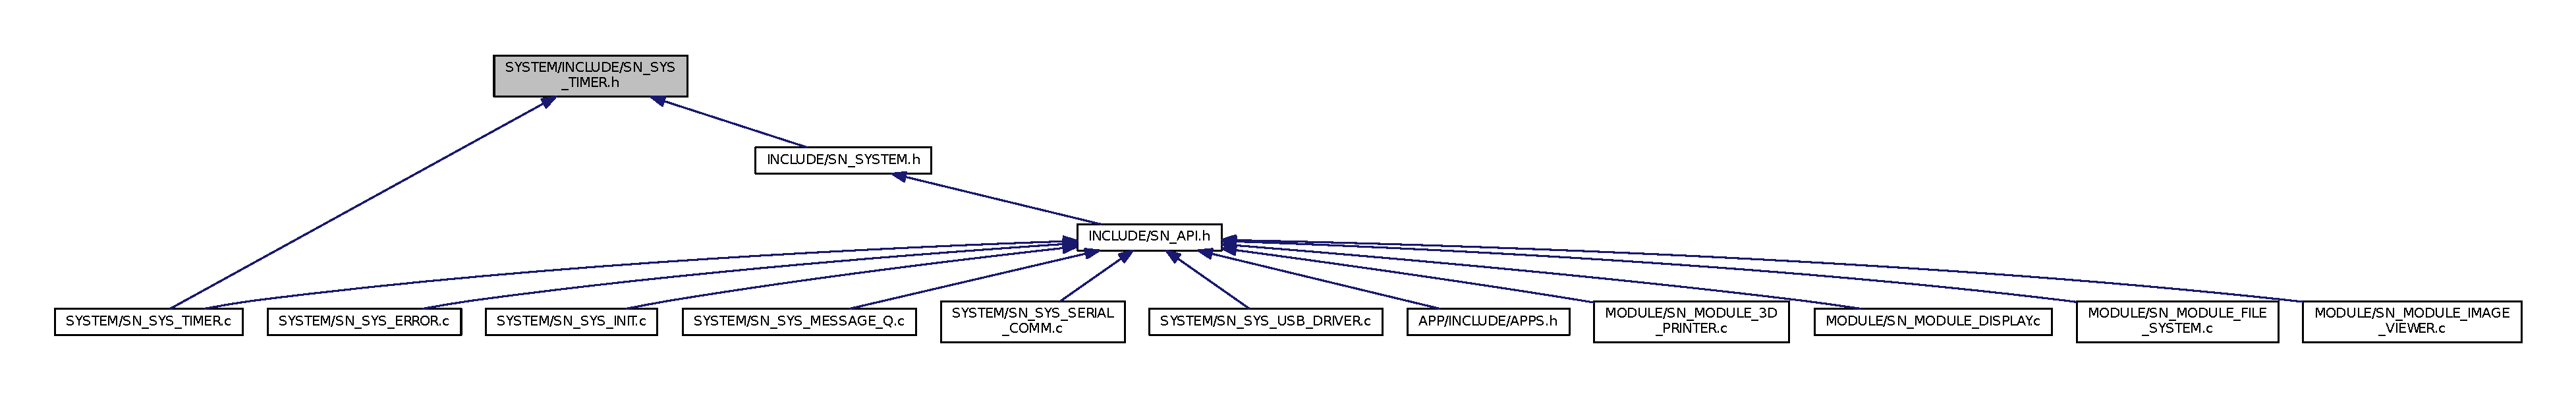
\includegraphics[width=350pt]{SN__SYS__TIMER_8h__dep__incl}
\end{center}
\end{figure}
\subsection*{Classes}
\begin{DoxyCompactItemize}
\item 
struct \hyperlink{structsys__timer__id}{sys\+\_\+timer\+\_\+id}
\end{DoxyCompactItemize}
\subsection*{Macros}
\begin{DoxyCompactItemize}
\item 
\#define \hyperlink{group__SYSTEM__TIMER_gad99ad563a1a632fde508ad8be6422e57}{M\+A\+X\+\_\+\+N\+U\+M\+\_\+\+O\+F\+\_\+\+T\+SR}~32
\item 
\#define {\bfseries U\+N\+A\+L\+L\+O\+C\+A\+T\+E\+D\+\_\+\+T\+S\+R\+\_\+\+ID}~(0x\+F\+F\+F\+F\+F\+F\+F\+F)
\end{DoxyCompactItemize}
\subsection*{Typedefs}
\begin{DoxyCompactItemize}
\item 
typedef struct \hyperlink{structsys__timer__id}{sys\+\_\+timer\+\_\+id} {\bfseries sys\+Timer\+Q\+\_\+t}
\item 
typedef uint32\+\_\+t {\bfseries sys\+Timer\+Id\+\_\+t}
\end{DoxyCompactItemize}
\subsection*{Functions}
\begin{DoxyCompactItemize}
\item 
\hyperlink{group__SYSTEM__ERROR_ga4540713b9a7a18ce44d78c3a10f7442f}{S\+N\+\_\+\+S\+T\+A\+T\+US} {\bfseries S\+N\+\_\+\+S\+Y\+S\+\_\+\+Timer\+Init} (void)
\item 
\hyperlink{group__SYSTEM__ERROR_ga4540713b9a7a18ce44d78c3a10f7442f}{S\+N\+\_\+\+S\+T\+A\+T\+US} {\bfseries S\+N\+\_\+\+S\+Y\+S\+\_\+\+Timer\+Create} (sys\+Timer\+Id\+\_\+t $\ast$p\+Id\+T\+SR, unsigned int ms\+Duration, void $\ast$pf\+T\+SR)
\item 
\hyperlink{group__SYSTEM__ERROR_ga4540713b9a7a18ce44d78c3a10f7442f}{S\+N\+\_\+\+S\+T\+A\+T\+US} {\bfseries S\+N\+\_\+\+S\+Y\+S\+\_\+\+Timer\+Cancle} (sys\+Timer\+Id\+\_\+t $\ast$p\+Id\+T\+SR)
\item 
\hyperlink{group__SYSTEM__ERROR_ga4540713b9a7a18ce44d78c3a10f7442f}{S\+N\+\_\+\+S\+T\+A\+T\+US} {\bfseries S\+N\+\_\+\+S\+Y\+S\+\_\+\+Delay} (uint32\+\_\+t msec)
\end{DoxyCompactItemize}


\subsection{Detailed Description}
\begin{DoxyAuthor}{Author}
Bato 
\end{DoxyAuthor}
\begin{DoxyDate}{Date}
18 Sep 2018 
\end{DoxyDate}
\begin{DoxySeeAlso}{See also}
\href{http://www.stack.nl/~dimitri/doxygen/docblocks.html}{\tt http\+://www.\+stack.\+nl/$\sim$dimitri/doxygen/docblocks.\+html} 

\href{http://www.stack.nl/~dimitri/doxygen/commands.html}{\tt http\+://www.\+stack.\+nl/$\sim$dimitri/doxygen/commands.\+html} 
\end{DoxySeeAlso}


���}	� �
����DEV��INO��SYN��SV~�#`
#`
�#`
k��N6I]�[~-
\hypertarget{SN__SYS__ERROR_8c}{}\section{S\+Y\+S\+T\+E\+M/\+S\+N\+\_\+\+S\+Y\+S\+\_\+\+E\+R\+R\+OR.c File Reference}
\label{SN__SYS__ERROR_8c}\index{S\+Y\+S\+T\+E\+M/\+S\+N\+\_\+\+S\+Y\+S\+\_\+\+E\+R\+R\+O\+R.\+c@{S\+Y\+S\+T\+E\+M/\+S\+N\+\_\+\+S\+Y\+S\+\_\+\+E\+R\+R\+O\+R.\+c}}
{\ttfamily \#include \char`\"{}S\+N\+\_\+\+A\+P\+I.\+h\char`\"{}}\newline
{\ttfamily \#include \char`\"{}S\+N\+\_\+\+S\+Y\+S\+\_\+\+E\+R\+R\+O\+R.\+h\char`\"{}}\newline
Include dependency graph for S\+N\+\_\+\+S\+Y\+S\+\_\+\+E\+R\+R\+O\+R.\+c\+:
\nopagebreak
\begin{figure}[H]
\begin{center}
\leavevmode
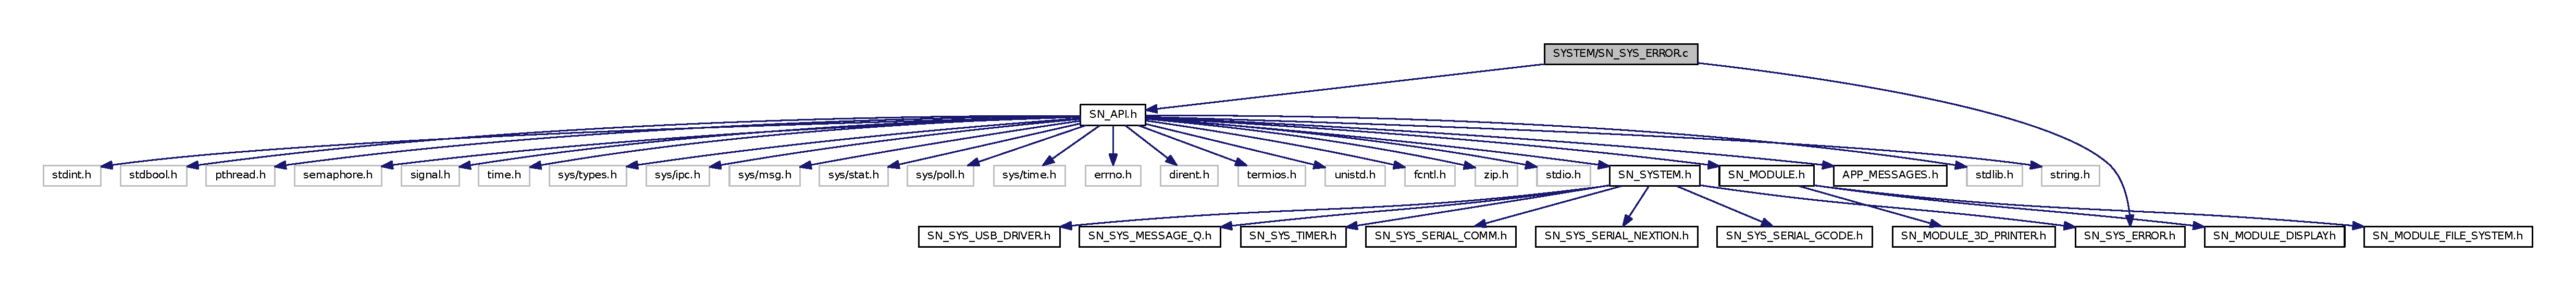
\includegraphics[width=350pt]{SN__SYS__ERROR_8c__incl}
\end{center}
\end{figure}
\subsection*{Functions}
\begin{DoxyCompactItemize}
\item 
\mbox{\Hypertarget{SN__SYS__ERROR_8c_aa8a811135aa795c5745e00a29424ab24}\label{SN__SYS__ERROR_8c_aa8a811135aa795c5745e00a29424ab24}} 
void {\bfseries s\+Reboot} (void)
\item 
\mbox{\Hypertarget{SN__SYS__ERROR_8c_a92c7beb3f46c22fdeed0ce55421b91e1}\label{SN__SYS__ERROR_8c_a92c7beb3f46c22fdeed0ce55421b91e1}} 
void {\bfseries s\+Exit} (void)
\item 
void \hyperlink{group__SYSTEM__ERROR_ga0a87cb464a83646bf30c20c867754a02}{S\+N\+\_\+\+S\+Y\+S\+\_\+\+Error\+Check} (\hyperlink{group__SYSTEM__ERROR_ga4540713b9a7a18ce44d78c3a10f7442f}{S\+N\+\_\+\+S\+T\+A\+T\+US} error\+Status, const char $\ast$error\+Message, const char $\ast$\+\_\+file, const char $\ast$\+\_\+func, const int \+\_\+line)
\item 
void \hyperlink{group__SYSTEM__ERROR_gaacf422ec9176edcc5b0d803da0b567b7}{S\+N\+\_\+\+S\+Y\+S\+\_\+\+Log} (const char $\ast$message)
\end{DoxyCompactItemize}


\subsection{Detailed Description}
\begin{DoxyAuthor}{Author}
Bato 
\end{DoxyAuthor}
\begin{DoxyDate}{Date}
24 Sep 2018 
\end{DoxyDate}
\begin{DoxySeeAlso}{See also}
\href{http://www.stack.nl/~dimitri/doxygen/docblocks.html}{\tt http\+://www.\+stack.\+nl/$\sim$dimitri/doxygen/docblocks.\+html} 

\href{http://www.stack.nl/~dimitri/doxygen/commands.html}{\tt http\+://www.\+stack.\+nl/$\sim$dimitri/doxygen/commands.\+html} 
\end{DoxySeeAlso}

\hypertarget{SN__SYS__INIT_8c}{}\section{S\+Y\+S\+T\+E\+M/\+S\+N\+\_\+\+S\+Y\+S\+\_\+\+I\+N\+IT.c File Reference}
\label{SN__SYS__INIT_8c}\index{S\+Y\+S\+T\+E\+M/\+S\+N\+\_\+\+S\+Y\+S\+\_\+\+I\+N\+I\+T.\+c@{S\+Y\+S\+T\+E\+M/\+S\+N\+\_\+\+S\+Y\+S\+\_\+\+I\+N\+I\+T.\+c}}
{\ttfamily \#include \char`\"{}S\+N\+\_\+\+A\+P\+I.\+h\char`\"{}}\newline
Include dependency graph for S\+N\+\_\+\+S\+Y\+S\+\_\+\+I\+N\+I\+T.\+c\+:\nopagebreak
\begin{figure}[H]
\begin{center}
\leavevmode
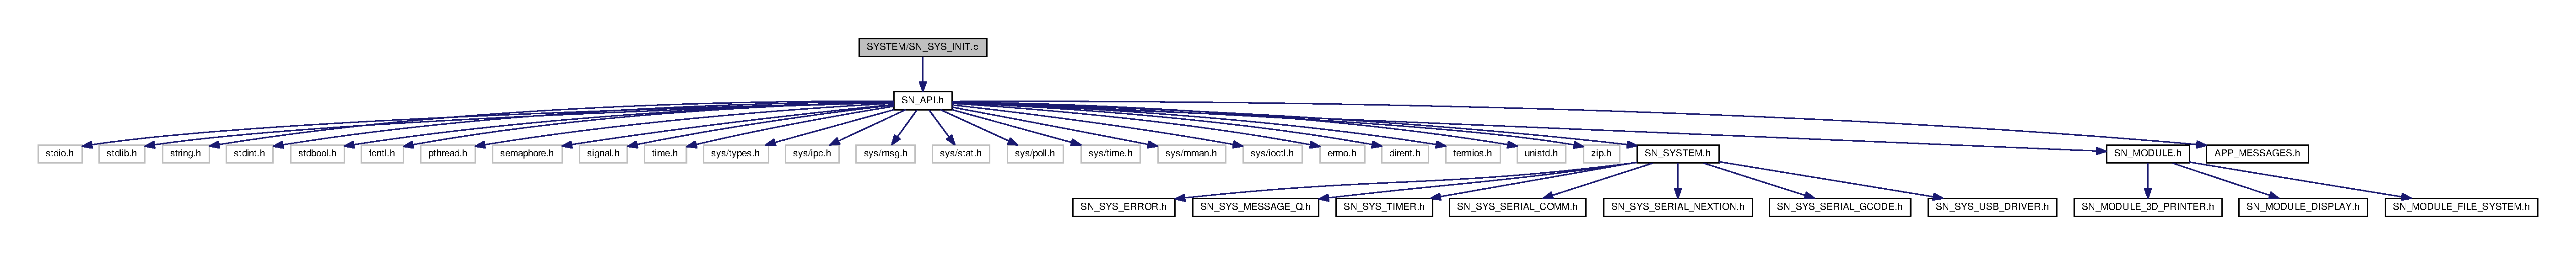
\includegraphics[width=350pt]{SN__SYS__INIT_8c__incl}
\end{center}
\end{figure}
\subsection*{Functions}
\begin{DoxyCompactItemize}
\item 
\mbox{\Hypertarget{SN__SYS__INIT_8c_a0eeea6b80bdc1c174e66709e41bf7634}\label{SN__SYS__INIT_8c_a0eeea6b80bdc1c174e66709e41bf7634}} 
\hyperlink{group__SYSTEM__ERROR_ga4540713b9a7a18ce44d78c3a10f7442f}{S\+N\+\_\+\+S\+T\+A\+T\+US} {\bfseries A\+P\+P\+\_\+\+Main} (\hyperlink{structgeneral__event}{general\+\_\+evt\+\_\+t} evt)
\item 
\mbox{\Hypertarget{SN__SYS__INIT_8c_ab175a483c4dccb76fb5835b4166b3a62}\label{SN__SYS__INIT_8c_ab175a483c4dccb76fb5835b4166b3a62}} 
\hyperlink{group__SYSTEM__ERROR_ga4540713b9a7a18ce44d78c3a10f7442f}{S\+N\+\_\+\+S\+T\+A\+T\+US} {\bfseries A\+P\+P\+\_\+\+Init} (void)
\item 
\mbox{\Hypertarget{SN__SYS__INIT_8c_a840291bc02cba5474a4cb46a9b9566fe}\label{SN__SYS__INIT_8c_a840291bc02cba5474a4cb46a9b9566fe}} 
int \hyperlink{SN__SYS__INIT_8c_a840291bc02cba5474a4cb46a9b9566fe}{main} (void)
\begin{DoxyCompactList}\small\item\em main \end{DoxyCompactList}\item 
\hyperlink{group__SYSTEM__ERROR_ga4540713b9a7a18ce44d78c3a10f7442f}{S\+N\+\_\+\+S\+T\+A\+T\+US} \hyperlink{group__APP__MSG_gaaecff3f61e5dd381bf5088743ec6d3df}{S\+N\+\_\+\+S\+Y\+S\+T\+E\+M\+\_\+\+Send\+App\+Message} (event\+\_\+id\+\_\+t evt\+Id, event\+\_\+msg\+\_\+t evt\+Message)
\end{DoxyCompactItemize}
\subsection*{Variables}
\begin{DoxyCompactItemize}
\item 
\mbox{\Hypertarget{SN__SYS__INIT_8c_a4301ccc1a555b4aac39b4ecd28081e0b}\label{SN__SYS__INIT_8c_a4301ccc1a555b4aac39b4ecd28081e0b}} 
\hyperlink{structsys__message__queue}{sys\+Message\+Q\+Id} {\bfseries msg\+Q\+Id\+App}
\end{DoxyCompactItemize}


\subsection{Detailed Description}
\begin{DoxyAuthor}{Author}
Bato 
\end{DoxyAuthor}
\begin{DoxyDate}{Date}
18 Sep 2018 
\end{DoxyDate}
\begin{DoxySeeAlso}{See also}
\href{https://bitbucket.org/xengiennering/sn3d-project/src/master/}{\tt https\+://bitbucket.\+org/xengiennering/sn3d-\/project/src/master/} 

\href{http://www.stack.nl/~dimitri/doxygen/docblocks.html}{\tt http\+://www.\+stack.\+nl/$\sim$dimitri/doxygen/docblocks.\+html} 

\href{http://www.stack.nl/~dimitri/doxygen/commands.html}{\tt http\+://www.\+stack.\+nl/$\sim$dimitri/doxygen/commands.\+html} 
\end{DoxySeeAlso}

\hypertarget{SN__SYS__MESSAGE__Q_8c}{}\section{S\+Y\+S\+T\+E\+M/\+S\+N\+\_\+\+S\+Y\+S\+\_\+\+M\+E\+S\+S\+A\+G\+E\+\_\+Q.c File Reference}
\label{SN__SYS__MESSAGE__Q_8c}\index{S\+Y\+S\+T\+E\+M/\+S\+N\+\_\+\+S\+Y\+S\+\_\+\+M\+E\+S\+S\+A\+G\+E\+\_\+\+Q.\+c@{S\+Y\+S\+T\+E\+M/\+S\+N\+\_\+\+S\+Y\+S\+\_\+\+M\+E\+S\+S\+A\+G\+E\+\_\+\+Q.\+c}}
{\ttfamily \#include \char`\"{}S\+N\+\_\+\+A\+P\+I.\+h\char`\"{}}\newline
{\ttfamily \#include \char`\"{}S\+N\+\_\+\+S\+Y\+S\+\_\+\+M\+E\+S\+S\+A\+G\+E\+\_\+\+Q.\+h\char`\"{}}\newline
Include dependency graph for S\+N\+\_\+\+S\+Y\+S\+\_\+\+M\+E\+S\+S\+A\+G\+E\+\_\+\+Q.\+c\+:\nopagebreak
\begin{figure}[H]
\begin{center}
\leavevmode
\includegraphics[width=350pt]{SN__SYS__MESSAGE__Q_8c__incl}
\end{center}
\end{figure}
\subsection*{Functions}
\begin{DoxyCompactItemize}
\item 
\hyperlink{group__SYSTEM__ERROR_ga4540713b9a7a18ce44d78c3a10f7442f}{S\+N\+\_\+\+S\+T\+A\+T\+US} \hyperlink{group__SYSTEM__MESSAGE__Q_ga35e9ff084626dfccd36d098827638a0c}{S\+N\+\_\+\+S\+Y\+S\+\_\+\+Message\+Q\+Init} (\hyperlink{structsys__message__queue}{sys\+Message\+Q\+Id} $\ast$msg\+Q\+Id)
\item 
\hyperlink{group__SYSTEM__ERROR_ga4540713b9a7a18ce44d78c3a10f7442f}{S\+N\+\_\+\+S\+T\+A\+T\+US} \hyperlink{group__SYSTEM__MESSAGE__Q_ga293a77ea597b70f3f2f38b919f93497e}{S\+N\+\_\+\+S\+Y\+S\+\_\+\+Message\+Q\+Remove} (\hyperlink{structsys__message__queue}{sys\+Message\+Q\+Id} $\ast$msg\+Q\+Id)
\item 
\hyperlink{group__SYSTEM__ERROR_ga4540713b9a7a18ce44d78c3a10f7442f}{S\+N\+\_\+\+S\+T\+A\+T\+US} \hyperlink{group__SYSTEM__MESSAGE__Q_ga36e115419d4cbbfe4a6bde6e3fecf180}{S\+N\+\_\+\+S\+Y\+S\+\_\+\+Message\+Put} (\hyperlink{structsys__message__queue}{sys\+Message\+Q\+Id} $\ast$msg\+Q\+Id, event\+\_\+id\+\_\+t evt\+Id, event\+\_\+msg\+\_\+t evt\+Message)
\item 
\hyperlink{structgeneral__event}{general\+\_\+evt\+\_\+t} \hyperlink{group__SYSTEM__MESSAGE__Q_gafb2da611b3c93f1f906109e7737d67cf}{S\+N\+\_\+\+S\+Y\+S\+\_\+\+Message\+Get} (\hyperlink{structsys__message__queue}{sys\+Message\+Q\+Id} $\ast$msg\+Q\+Id)
\end{DoxyCompactItemize}


\subsection{Detailed Description}
\begin{DoxyAuthor}{Author}
Bato 
\end{DoxyAuthor}
\begin{DoxyDate}{Date}
16 Oct 2018 
\end{DoxyDate}
\begin{DoxySeeAlso}{See also}
\href{http://www.stack.nl/~dimitri/doxygen/docblocks.html}{\tt http\+://www.\+stack.\+nl/$\sim$dimitri/doxygen/docblocks.\+html} 

\href{http://www.stack.nl/~dimitri/doxygen/commands.html}{\tt http\+://www.\+stack.\+nl/$\sim$dimitri/doxygen/commands.\+html} 
\end{DoxySeeAlso}


���}	� �
����DEV��INO��SYN��SV~�#`
#`
�#`
k��Y�I]�[��

���}	� �
����DEV��INO��SYN��SV~�#`
#`
�#`
k��[�I]�[��
\hypertarget{SN__SYS__USB__DRIVER_8c}{}\section{S\+Y\+S\+T\+E\+M/\+S\+N\+\_\+\+S\+Y\+S\+\_\+\+U\+S\+B\+\_\+\+D\+R\+I\+V\+ER.c File Reference}
\label{SN__SYS__USB__DRIVER_8c}\index{S\+Y\+S\+T\+E\+M/\+S\+N\+\_\+\+S\+Y\+S\+\_\+\+U\+S\+B\+\_\+\+D\+R\+I\+V\+E\+R.\+c@{S\+Y\+S\+T\+E\+M/\+S\+N\+\_\+\+S\+Y\+S\+\_\+\+U\+S\+B\+\_\+\+D\+R\+I\+V\+E\+R.\+c}}
{\ttfamily \#include \char`\"{}S\+N\+\_\+\+A\+P\+I.\+h\char`\"{}}\newline
{\ttfamily \#include \char`\"{}S\+N\+\_\+\+S\+Y\+S\+\_\+\+U\+S\+B\+\_\+\+D\+R\+I\+V\+E\+R.\+h\char`\"{}}\newline
Include dependency graph for S\+N\+\_\+\+S\+Y\+S\+\_\+\+U\+S\+B\+\_\+\+D\+R\+I\+V\+E\+R.\+c\+:
\nopagebreak
\begin{figure}[H]
\begin{center}
\leavevmode
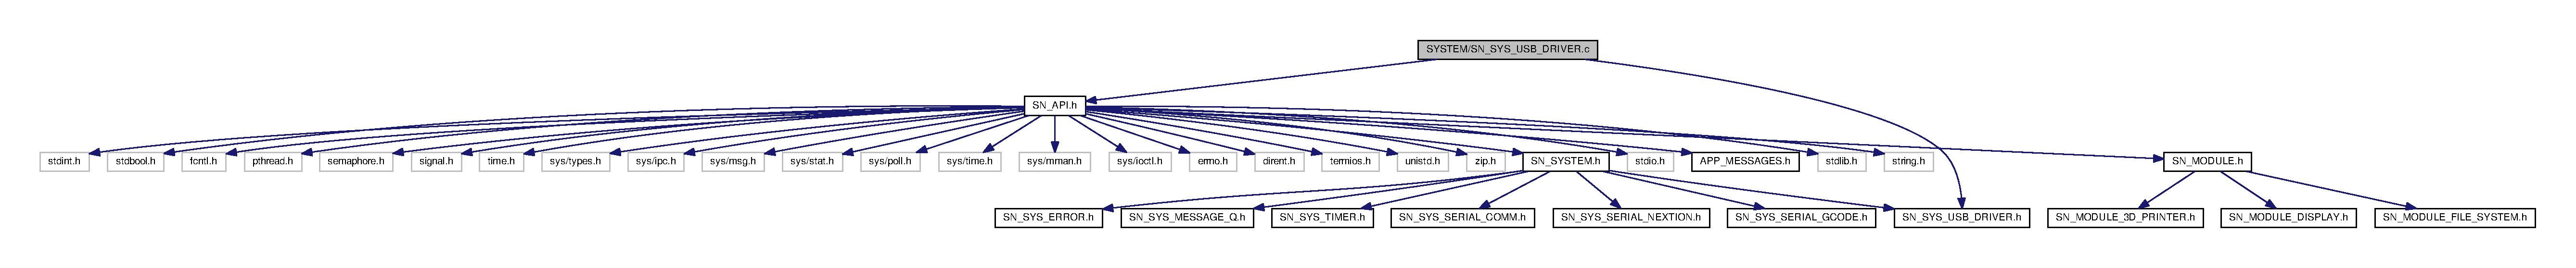
\includegraphics[width=350pt]{SN__SYS__USB__DRIVER_8c__incl}
\end{center}
\end{figure}
\subsection*{Macros}
\begin{DoxyCompactItemize}
\item 
\mbox{\Hypertarget{SN__SYS__USB__DRIVER_8c_a748b5b8cef6b34b348684975c5d0578c}\label{SN__SYS__USB__DRIVER_8c_a748b5b8cef6b34b348684975c5d0578c}} 
\#define {\bfseries U\+S\+B\+\_\+\+U\+N\+M\+O\+U\+NT}~0
\item 
\mbox{\Hypertarget{SN__SYS__USB__DRIVER_8c_ac0641099c07ba1f6ad852306aadb0032}\label{SN__SYS__USB__DRIVER_8c_ac0641099c07ba1f6ad852306aadb0032}} 
\#define {\bfseries U\+S\+B\+\_\+\+M\+O\+U\+NT}~1
\end{DoxyCompactItemize}
\subsection*{Functions}
\begin{DoxyCompactItemize}
\item 
\hyperlink{group__SYSTEM__ERROR_ga4540713b9a7a18ce44d78c3a10f7442f}{S\+N\+\_\+\+S\+T\+A\+T\+US} \hyperlink{group__SYSTEM__USB__DRIVER_gaf7719b8e9f6d6f05b702ac7d4e9c5a61}{S\+N\+\_\+\+S\+Y\+S\+\_\+\+U\+S\+B\+Driver\+Init} (void $\ast$(pf\+Call\+Back)(int evt))
\item 
\hyperlink{group__SYSTEM__ERROR_ga4540713b9a7a18ce44d78c3a10f7442f}{S\+N\+\_\+\+S\+T\+A\+T\+US} \hyperlink{group__SYSTEM__USB__DRIVER_ga60bc7a83a5370d89dffe6e3d4ad88538}{S\+N\+\_\+\+S\+Y\+S\+\_\+\+U\+S\+B\+Driver\+Terminate} (void)
\item 
bool \hyperlink{group__SYSTEM__USB__DRIVER_gaccafd3f2c96104a41f768f05a083226f}{S\+N\+\_\+\+S\+Y\+S\+\_\+\+U\+S\+B\+Driver\+Is\+Mount} (void)
\end{DoxyCompactItemize}


\subsection{Detailed Description}
\begin{DoxyAuthor}{Author}
Bato 
\end{DoxyAuthor}
\begin{DoxyDate}{Date}
18 Sep 2018 
\end{DoxyDate}
\begin{DoxySeeAlso}{See also}
\href{http://www.stack.nl/~dimitri/doxygen/docblocks.html}{\tt http\+://www.\+stack.\+nl/$\sim$dimitri/doxygen/docblocks.\+html} 

\href{http://www.stack.nl/~dimitri/doxygen/commands.html}{\tt http\+://www.\+stack.\+nl/$\sim$dimitri/doxygen/commands.\+html}
\end{DoxySeeAlso}
\begin{DoxyRefDesc}{Bug}
\item[\hyperlink{bug__bug000002}{Bug}]U\+S\+B\+\_\+\+U\+N\+M\+O\+U\+N\+T\+\_\+\+E\+V\+E\+NT not working \end{DoxyRefDesc}

%--- End generated contents ---

% Index
\backmatter
\newpage
\phantomsection
\clearemptydoublepage
\addcontentsline{toc}{chapter}{Index}
\printindex

\end{document}
